% ******************************************************************************
%
% Diese Hauptdatei beinhaltet  Kapitel der Dokumentation.
% ******************************************************************************
% ******************************************************************************
%
% Laden der Dokumentenklasse Report
\documentclass[%
    a4paper,        % Papiergroesse
    nexus,          % Schriftart [nexus,arial]
    11pt,           % Schriftgroesse
    lnum,           % Die Paket-/Klassenoption lnum wählt für das Dokument einen
                    % Schriftschnitt mit Versalziffern.
    smallchapters,  % Stellt kleinere Chapter Ueberschriften ein.
    oneside,        %
    %halfparskip,   %
    %fleqn,         % Gleichungen werden links ausgerichtet
    %style=screen,   % Für die bessere Darstellung auf dem Bildschirm. Fuer den
                    % Druck entfernen.
    %monochrome,
    rgb,
    svgnames,       % Laden von Farbnamen vordefinierter Farben aus xcolor
    parskip=full,	% Absaetze statt Einzug
]{tubsreprt}        % Definition der Dokumentenklasse
% ******************************************************************************
%
% Laden der noetigen Latex Pakete, sowie Einstellungen im Praeamble, die fuer
% das Dokument benoetigt werden. Dort wird auch das Paket mit den eigenen Makros
% geladen.
% ******************************************************************************
%
% Es ist zu beachten, dass bei einer Vielzahl an geladenen Paketen der Compiler
% folgende Fehlermeldung "! No room for a new \dimen ." ausgibt, wenn ein
% Zaehler 233 Register allokiert hat. Zuerst muss das Paket morewrites and etex
% geladen werden, um eine hoehere Anzahl Schreibregister zu ermoeglichen, da
% ansonsten nur 256 Register bereitstehen. Mit etex stehen 32768 Register zur
% Verfuegung. Siehe hierzu:
% http://tex.stackexchange.com/questions/38607/no-room-for-a-new-dimen
\usepackage{morewrites}
% see http://www.tex.ac.uk/cgi-bin/texfaq2html?label=noroom
% After update for LaTeX released after 2015 not rquired anymore. Activate for
% previous version.
% For more Informationi see:
% https://tex.stackexchange.com/questions/38607/no-room-for-a-new-dimen
%\usepackage{etex}
%\reserveinserts{28}
% ******************************************************************************
%
% Pruefung des Textes mit neuer deutscher Rechtschreibung
\usepackage[ngerman]{babel}
%
% Uebersetzt unterschiedliche Begriffe, die in LaTeX vorhanden sind bei der
% Ausgabe in das Deutsche.
% Beispielsweise: \SI{1.234}{\metre}
\usepackage[ngerman]{translator}
% ******************************************************************************
%
% Das inputenc-Paket ermoeglicht die direkte Eingabe von Sonderzeichen.
\usepackage[utf8]{inputenc}
% ******************************************************************************
%
% Biber Paket fuer die Literaturliste
%\usepackage{multibib}
\usepackage[backend=biber]{biblatex}
%\usepackage[
%    backend=biber,
%    style=authoryear-icomp,
%    sortlocale=de_DE,
%    natbib=true,
%    url=false,
%    doi=true,
%    eprint=false,
%    bibencoding=utf8,safeinputenc=true
%]{biblatex}
\addbibresource{Literatur.bib}
% \bibliography{Literatur}
% ******************************************************************************
%
% Textsatz
%
% Das microtype-Paket bringt optischen Randausgleich und minimale Skalierung der
% Buchstaben. Diese »font-expansion« verbessert den Zeilenumbruch, reduziert
% Trennstellen und erhoeht den Grauwert der Seite. Es werden Wortzwischenraeume
% im Blocksatz gleichmaessiger. Die Zeit eines bei der Erstellung der tex
% Dokumentes verlaengert sich, da die Schriftart-Varianten berechnet werden
% muessen. Seit 2007 kann das Paket sich auch automatisch um die leichte
% Sperrung von Kapitaelchen kuemmern. Mit diesem Paket wird die Anzahl von
% "under-" und "overfull box" Warnungen innerhalb der Kompilierungs Logdateien
% verringert.
\usepackage{microtype}
%
% Das winzige Paket ellipsis kuemmert sich um den Leerraum rund um die
% Auslassungspunkte. Es kann bedenkenlos immer geladen werden.
\usepackage{ellipsis}
%
% Schusterjungen und Witwenregelung
% Verhindert einzelne erste Zeilen unten
\clubpenalty = 10000
% Verhindert einzelne letzte Zeilen oben
\widowpenalty = 10000
\displaywidowpenalty = 10000
%
% Dieses Paket hilft die Zeilenabstaende dynamisch anzupassen. Eine andere Art
% um Zeilenabstaende im Text zu definieren. Mit \onehalfspacing wird
% Zeilenabstand auf 1.5 gesetzt.
%\usepackage{setspace}
%
% Mit dem \parskip Befehl und einer Laengenangabe ist es moeglich die Groesse
% eines Absatzes zu bestimmen.
%\usepackage{parskip}
% ******************************************************************************
%
% Formatierungen
%
% Erscheinungsbild der Bild- und Tabellenbeschriftung anpassen
\usepackage[hang,small,bf]{caption}
%
% Entfernt das Einbinden der ToC (Table of Contents)
\usepackage[nottoc]{tocbibind}
% ******************************************************************************
%
% Pakete, die fuer die Darstellung mathematischer Gleichungen notwendig sind
\usepackage[tbtags]{amsmath}
\usepackage{amsfonts}
\usepackage{amssymb}
\usepackage{mathtools}
%
\usepackage{commath}
%
\usepackage{bm}
%
% Streichen von Termen zu einem Wert, beispielsweise ->0
%\usepackage[
%    smaller,
%    %makeroom
%]{cancel}
%
% Ermoeglicht die fleqn Umgebung, um einzelne Gleichungen linksbuendig
% darzustellen.
% Aufgrund von einem zuvor definierten \nr Makro, steht es im Konflikt mit
% dem Paket nccmath.
%\let\oldnr=\nr
%\let\nr\undefined
%
%\usepackage{nccmath}
%
% Erlaube Zerilenumbrueche in Formeln
%\allowdisplaybreaks
%
% Erzeuge einen Operator Rang
%\DeclareMathOperator{\Rang}{Rang}
% Vektorpfeil mit \vv{} darstellen
%\usepackage{esvect}
%\MakeRobust{\vv}
% ******************************************************************************
%
% Paket, um Werte und Einheiten darzustellen und Tabellen mit Ziffern zu
% Formatieren.
\usepackage{siunitx}
%
% Einstellungen fuer eine deutsche Ausgabe
\sisetup{output-decimal-marker = {,}}
\sisetup{locale = DE}
\sisetup{per-mode = symbol}
%
% Laden von Abkuerzungen
\sisetup{load-configurations = abbreviations}
%\sisetup{load=prefixed}
% ******************************************************************************
%
% Das Paket ermoeglicht das erstellen von Glossaries und Abkuerzungen, sowie
% Abkuerzungen von Formelzeichen.
\usepackage[
    nonumberlist,   % keine Seitenzahlen anzeigen
    acronym,        % ein Abkuerzungsverzeichnis erstellen
    %toc,           % Eintraege im Inhaltsverzeichnis
    %nottoc,
    section,        % Im Inhaltsverzeichnis auf section-Ebene erscheinen
    %footnote        % Erklaerungen und ausgeschriebene Abkürzungen beim ersten
                    % erscheinen als Fußnote
]{glossaries}
% ******************************************************************************
%
% Sonderzeichen
%
% Erlaubt dei Verwendung von Sonderzeichen. Importiert beispielsweise das
% Promill Zeichen.
%\usepackage{textcomp}
%
% Dieses Paket laedt erweiterte Symbole
%\usepackage{latexsym}
%
% Weitere Sonderzeichen und Symbole
%\usepackage{pifont}
%
% @ wird als Buchstabe interpretiert
%\makeatletter
% ******************************************************************************
%
% Allgemein benoetigte Pakete
%
% Internetadressen direkt verlinken. Einfuegen von URLs mit:
% \url{http://www.Seitennahme.de/}
%\usepackage{url}
%
% Erlaubt Unterstreichen mit \uline, \uuline \uwave usw.
%\usepackage{ulem}
%EXAMPLE UNDERLINE
%\underline{\smash{The quick brown fox jumped over the lazy dog.}}
%\setul{5pt}{.4pt}% 5pt below contents
%\ul{The quick brown fox jumped over the lazy dog.} \par
%\setul{1pt}{.4pt}% 1pt below contents
%\ul{The quick brown fox jumped over the lazy dog.} \par
%
% Dieses Paket wird benoetigt, um stellenweise Querformat nutzen zu koennen.
% Genutzt wird das Querformat mit:
% \begin{landscape} Text \end{landscape}.
%\usepackage{lscape}
%
% Um Tabellen auf die breite der Seite zu bekommen, werden mit "X" markierte
% Spalten gestaucht, die anderen nicht
%\usepackage{tabularx}
%
% Erlaubt in Tabellen die Zusammenfassung mehrerer Spalten einer Zeile zu einer.
% Fuer die zusammengafsste Spalte ist im Gegensatz zu \multirow{}{}{} kein
% Leerfeld mittels "&" zu setzten.
%\usepackage{array,multicol}
%
% Aufzaehlungen
%\usepackage{enumitem}
%
% drehen Tab,Fig:\begin{sideways},\begin{rotate}{30}
\usepackage{rotating}
%\usepackage{hvfloat}
% ******************************************************************************
%
% Erweiterung zu color mit Zugriff auf verschiedene Arten
%\usepackage[svgnames,table]{xcolor}
% ******************************************************************************
%
% Allgemeine Darstellungen von Grafiken
%
% Wird benoetigt fuer die Darstellung von Grafiken.
\usepackage{graphicx}
%
% Stelle die Pfade fuer Grafiken zur Verfuegung
\graphicspath{{images/}{images/}}
%
% Mit diesem Paket und dem Befehl '\begin{figure}[H]' bzw. der Position [H],
% koennen Bilder genau an die Stelle im Text gesetzt werden, wo das Bild
% eingefuegt wird.
\usepackage{float}
%
% Ermoeglicht das darstellen von vielen (unter) Bildern als ein Bild.
%\usepackage{subfigure}
\usepackage{subfig}
% ******************************************************************************
%
% Ermoeglicht das Einbinden von PDF Dateien.
\usepackage{pdfpages}
% ******************************************************************************
%
% Dieses Paket ermoeglicht PGF plots innerhalb der TIKZ Umgebung
\usepackage{pgf}
%
% Ermoeglicht eine Darstellung von (vielen) Werte in einem Diagramm mit
% unterschiedlichen Eigenschaften und vielen Funktionen.
\usepackage{pgfplots}
%
% Wahl der PGF Version.
\pgfplotsset{compat=newest}
%
%\usepgfplotslibrary{external}
%
% Einstellen des Gleitzahltrennzeichens in PGF plots als Komma (deutsch)
\pgfplotsset{/pgf/number format/set decimal separator={,}}
%
\pgfplotsset{
    every axis/.append style={
        %line width=1pt,
        grid style={line width=1.0pt},
        tick style={line width=1.0pt, black}
    }
}
%
% Ermoeglicht den Zugriff auf das Paket \usepackage{siunitx} und die Verwendung
% von Einheiten innerhalb PGF Plots.
\usepgfplotslibrary{units}
%\usepgfplotslibrary{external}
%\tikzexternalize
%
% Spezieller Befehl, der eine Transformation von XY-Koordinaten des PGF
% Koordinatensystems in das Plot Koordinatensystem ermoeglicht.
%\makeatletter
%    \newcommand\transformxdimension[1]{
%        \pgfmathparse{%
%            ((#1/\pgfplots@x@veclength)+\pgfplots@data@scale@trafo@SHIFT@x)/%
%        10^\pgfplots@data@scale@trafo@EXPONENT@x}
%    }
%    \newcommand\transformydimension[1]{
%        \pgfmathparse{%
%            ((#1/\pgfplots@y@veclength)+\pgfplots@data@scale@trafo@SHIFT@y)/%
%       10^\pgfplots@data@scale@trafo@EXPONENT@y}
%    }
%\makeatother
% ******************************************************************************
%
% Tikz ermoeglicht das erstellen von Grafiken und Funktionsgraphen
% unterschiedlicher Art.
%
% Laden des Tikz Bild Format Paketes mit entsprechenden Bibliotheken.
\usepackage{tikz}
\usetikzlibrary{% Laden von unterschiedlichen TIKZ Bibliotheken.
    %shapes,
    %backgrounds,
    %shadows,
    %arrows,
    %matrix,
    %calc,
    positioning,
    %decorations.pathreplacing,
    %snakes,
%    intersections,
    %through,
    %patterns,
%    decorations.markings,
    %spy,                            % Ermoeglicht ein Zoomen in TIKZ Bildern
    %3d,
    %quotes,
    %angles,
    plotmarks
}
\tikzset{every picture/.append style={font=\small}}
\tikzset{
    every picture/.append style={
        line width=1.0pt,
        %thick,
        mark size=3pt
    }
}
%
% Erstelle die Tikz Bilder separat
% Nutze für pdflatex:  -shell-escape
%\usetikzlibrary{external}
%\tikzexternalize[prefix=figures/externalized/,shell escape=-enable-write18]
%\tikzset{external/system call={pdflatex
%     \tikzexternalcheckshellescape -halt-on-error -synctex=1
%     -file-line-error-style --shell-escape -extra-mem-top=20000000
%     -output-directory=build -interaction=batchmode -jobname "\image" "\texsource"}
%     }
%\tikzexternalize[prefix=fig_externalized/,
%	optimize=true, optimize command away=\includepdf,
%	%up to date check=diff,
%	up to date check=md5,
%]
%\tikzset{external/force remake}
%\tikzexternalize
%  *****************************************************************************
% Custom legend
% argument #1: any options
%\makeatletter
%\newenvironment{customlegend}[1][]{%
%    \begingroup
%    % inits/clears the lists (which might be populated from previous
%    % axes):
%    \pgfplots@init@cleared@structures
%    \pgfplotsset{#1}%
%}{%
%    % draws the legend:
%    \pgfplots@createlegend
%    \endgroup
%}%
%
%% makes \addlegendimage available (typically only available within an
%% axis environment):
%\def\addlegendimage{\pgfplots@addlegendimage}
%\makeatother
%  *****************************************************************************
%
% Werkzeuge zum Zeichnen euklidischer Geometrie.
%\usepackage{tkz-euclide}
%\usetkzobj{all}
%
% Tikz spezifisch Einstellungen
%
% Spy on plots
%\tikzset{%
%    new spy style/.style={%
%        spy scope={%
%            magnification=5,
%            size=1.25cm,
%            connect spies,
%            every spy on node/.style={%
%                rectangle,
%                draw,
%            },
%            every spy in node/.style={%
%                draw,
%                rectangle,
%                fill=gray!40,
%            }
%        }
%    }
%}
%
% Get X and Y out of an point in TIKZ
%\makeatletter
%\newcommand{\gettikzxy}[3]{%
%    \tikz@scan@one@point\pgfutil@firstofone#1\relax
%    \edef#2{\the\pgf@x}%
%    \edef#3{\the\pgf@y}%
%}
%
% ******************************************************************************
% Some default plotting lengths for figure sizes
%\makeatletter
%\newcommand{\figureheight}{%
%    \pagegoal \advance-\pagetotal
%}
%\def\@figureheight{
%    \dimexpr\pagegoal
    %\addtolength{\figureheight}{-\pagetotal}
    %\addtolength{\figureheight}{-\footskip}
%}
%\makeatother
\newlength\figurewidth
%\setlength{\figurewidth}{0.75\textwidth}
\setlength{\figurewidth}{0.9\textwidth}
\newlength\figureheigth
\setlength{\figureheigth}{0.75\textheight}
%
% twofigurewidth besitzt die laenge 0.5*(\textwidth-90pt)
% 90pt wird genutzt, da der pgf Plot zwei Axen mit jeweils einer Beschriftung
% haben kann.
\newlength\twofigurewidth
\setlength{\twofigurewidth}{\textwidth}
\addtolength{\twofigurewidth}{-45pt}
\setlength{\twofigurewidth}{0.5\twofigurewidth}
\newlength\twofigureheight
\setlength{\twofigureheight}{\textheight}
%\addtolength{\twofigureheight}{-45pt}
\setlength{\twofigureheight}{0.5\twofigureheight}
%
% twofigurewidth besitzt die laenge 0.5*(\textwidth-90pt)
% 90pt wird genutzt, da der pgf Plot zwei Axen mit jeweils einer Beschriftung
% haben kann.
\newlength\twofigurewidthxx
\setlength{\twofigurewidthxx}{\textwidth}
\addtolength{\twofigurewidthxx}{-45pt}
\setlength{\twofigurewidthxx}{0.5\twofigurewidthxx}
\newlength\twofigureheightxx
\setlength{\twofigureheightxx}{\textheight}
\addtolength{\twofigureheightxx}{-45pt}
\setlength{\twofigureheightxx}{0.5\twofigureheightxx}
%
% twofigurewidth besitzt die laenge 0.8*\twofigurewidth
\newlength\twofigurewidths
\setlength{\twofigurewidths}{0.80\twofigurewidth}
\newlength\twofigureheights
\setlength{\twofigureheight}{0.80\twofigureheight}
\newlength\threefigureheights
\setlength{\threefigureheights}{0.75\twofigureheight}
% ******************************************************************************
%
% Verlinkungen innerhalb des Dokumentes
%
\usepackage[
    breaklinks=true,
    colorlinks=false,
    %frenchlinks=false,
    %bookmarksnumbered=true
]{hyperref}                 % Package fuer Lesezeichen und Verlinkungen
% Beschreibung der Parameter
% breaklinks=boolean        : Gibt an, ob Links umgebrochen werden duerfen
% colorlinks=boolean        : Links eingefaerbt
% linkcolor=color           : Farbe der Dokument-internen Links
% citecolor=color           : Farbe der Links zum Literaturverzeichnis
% filecolor=color           : Farbe der Links auf lokale Dateien
% urlcolor=color            : Farbe der Links zu externe URLs
% frenchlinks=booelean      : Links werden als smallcaps, anstatt farbig
%                             dargestellt
% bookmarksnumbered=boolean : Kapitelnummern werden im Inhaltsverzeichnis
%                             angezeigt
\hypersetup{
    pdftitle    = {Berechnung von Pi},
    pdfsubject  = {Um was geht es \ldots},
    pdfauthor   = {Max Mustermann},
    pdfkeywords = {Rocket, Aerothermodynamics, Aerodynamics, flow Control},
    pdfcreator  = {pdflatex},
    pdfproducer = {LaTeX with hyperref}
}
% ******************************************************************************
%
% Einbinden von Tabellen
%
%\usepackage{csvsimple}
%
% Ermoeglicht das Erstellen von Tabellen ueber mehrere Seiten.
%\usepackage{longtable}
%
% Erstellen von Tabellen mit PGF
%\usepackage{pgfplotstable}
%
% Ermoeglicht den Import von *.csv Tabellen
%\usepackage{csvtools}
% Use ; seperators
%\setcsvseparator{,}
% Use tab seperators
%\setcsvseparator{^^I}
%
% Zusammenfassung mehrerer Reihen in einer Tabellenspalte
%\usepackage{multirow}
%
% Zusammenfassung mehrerer Spalten in einer Tabellenreihe
%\usepackage{multicolumn}
%
% Erzeugt hochwertigere horizontale Striche in Tabellen
%\usepackage{booktabs}
% ******************************************************************************
%
% Einstellungen fuer die Darstellung von Quelltexten
%
% ******************************************************************************
%
% Dieses Paket stellt die Befehle fuer die Gesamtzahl der Seiten, Abbildungen
% und Tabellen zur Verfuegung.
\usepackage[figure,table]{totalcount}
\usepackage{lastpage}
% ******************************************************************************
%
% Einbinden von eigenen Makros
%
\usepackage{my_macropackage}
% ******************************************************************************
%
% Ermoeglicht das erstellen von zu erledigenden TODO Notizen.
%
% Bei Fertigstellung sollte dieses Paket AUSKOMMENTIERT werden!
\usepackage{todonotes}
% ******************************************************************************
%
% Package for fenerating dummy text/blindtext
\usepackage{blindtext}
% ******************************************************************************
%
% Deklaration von Schriftarten für Formeln
\DeclareOldFontCommand{\rm}{\normalfont\rmfamily}{\mathrm}
\DeclareOldFontCommand{\sf}{\normalfont\sffamily}{\mathsf}
\DeclareOldFontCommand{\tt}{\normalfont\ttfamily}{\mathtt}
\DeclareOldFontCommand{\bf}{\normalfont\bfseries}{\mathbf}
\DeclareOldFontCommand{\it}{\normalfont\itshape}{\mathit}
\DeclareOldFontCommand{\sl}{\normalfont\slshape}{\@nomath\sl}
\DeclareOldFontCommand{\sc}{\normalfont\scshape}{\@nomath\sc}
\DeclareRobustCommand*\cal{\@fontswitch\relax\mathcal}
\DeclareRobustCommand*\mit{\@fontswitch\relax\mathnormal}
% ******************************************************************************
%
% Packages zum Erstellen von Struktogrammen
\usepackage{struktex}
%*******************************************************************************
% Packages zum einfachen Erstellen einer Projektdokumentierung, Workpackagedescription, Workbreakdownstructure und Gantt-Chart

\usepackage{lscape}

%
% Dieses Paket ermoeglicht PGF plots innerhalb der TIKZ Umgebung
\usepackage{pgf}
\usepackage{pgfgantt}
%
% Ermoeglicht ein viel einfacheres erstellen von WPDs
\usepackage{colortbl}
\usepackage{totcount}
\let\titleoriginal\title           % save original \title macro
\renewcommand{\title}[1]{          % substitute for a new \title
    \titleoriginal{#1}%               % define the real title
    \newcommand{\otitle}{#1}        % define \otitle
}
\usepackage{workpackagedescription}

\usepackage{tikz}

\usetikzlibrary{ shapes, shadows, arrows}
%*******************************************************************************
%
% ******************************************************************************
%
% Aendern der Nummerierung von arabisch auf roemisch
\pagenumbering{Roman}
%
% Der Textteil des LaTeX-Dokuments beginnt ab hier.
\begin{document}
    % **************************************************************************
    %
    % Einstellen und laden der Titelseite
    %
    % Titelseiten-Elemente
    \newcommand{\typeOfThesis}{Bachelorarbeit}
    \newcommand{\examiner}{Prof. Dr.-Ing. Peter Hecker}
    \newcommand{\supervisor}{Yannic Beyer, M. Sc.}
   	\newcommand{\secondsupervisor}{Alexander Peuker, M. Sc.}
    \author{Lucas Schreer}
    \title{%
       Flugmechanische Untersuchung zum effizienten Aufstieg in die untere Stratosphäre mit elektrischen, propellergetriebenen Fluggeräten
    }
    \subtitle{}
    \logo{
        
\includegraphics{TUBS_logo_inst_IFF}%
    }
    \titleabstract{\lipsum[2]}
    %\titlepicture{infozentrum.jpg}
    %
    % Rückseiten-Elemente
    \address{%
	    Technische Universit\"{a}t Braunschweig\\
        Institut f\"ur Flugf\"uhrung\\
        Hermann-Blenk-Str. 27\\
        D-38108 Braunschweig
    }
    \backpageinfo{%
        here comes some backpageinfo
    }
    %
    % Laden der Titelseite.
%    \tikzexternalenable
    %\include{title_page_report}
    % ******************************************************************************
% Datei       : title_page.tex
% ******************************************************************************
\begin{titlepage}
% ******************************************************************************
    \makeatletter
    \showtubslogo[left]
    \showlogo{\tubs@tp@logo}
    \showtopline
    % **************************************************************************
    \begin{titlerow}{1}
        \begin{center}
            %\sffamily%
            {\usekomafont{title}\typeOfThesis\par}%
        \end{center}
    \end{titlerow}
    \begin{titlerow}{2}
        \begin{center}
            \sffamily%
            {\usekomafont{chapter}\@title\par}\bigskip%
            \vfill%
            {\usekomafont{subtitle}\@subtitle}\bigskip%
            \vfill\vfill%
            {\usekomafont{author}\@author}\bigskip%%
            \vfill
            {\noindent\usekomafont{date}\@date}%
        \end{center}
    \end{titlerow}
    \begin{titlerow}{1}
    \end{titlerow}
    % **************************************************************************
    \begin{titlerow}{1}
        \begin{tabular}{ll}
        Prüfer: & \examiner\\
        Betreuer: & \supervisor
        \end{tabular}
    \end{titlerow}
    % **************************************************************************
    \begin{titlerow}{2}
        \begin{minipage}{0.6\textwidth}
            \begin{flushleft}
                %\traddress
                \tubs@tp@address
            \end{flushleft}
        \end{minipage}
        % **********************************************************************
        \begin{minipage}{0.3\textwidth}
            \begin{flushright}
                \begin{tabular}{lr}
                    Seiten: & \pageref{LastPage} \\
                    Abbildungen: & \totalfigures \\
                    Tabellen:  & \totaltables\\
                \end{tabular}
            \end{flushright}
        \end{minipage}
    % **************************************************************************
    \end{titlerow}
    %\showdesignhelper
    \makeatother
%% ******************************************************************************
\end{titlepage}
% ******************************************************************************

%    \tikzexternaldisable
    %
    
\includepdf[pages=-]{BA_Lucas_Schreer_Aufgabenstellung}
    %
    %%%%%%%%%%%%%%%%%%%%%%%%%%% 
	% Remove after finished !!!!!!!!!!!!!!!!!!!!!!!!!
%	\todototoc  
%    \listoftodos
	%%%%%%%%%%%%%%%%%%%%%%%%%%%
    % Einbinden des Eids.
    \chapter*{Eidesstattliche Erkl\"arung}

Ich erkläre hiermit an Eides Statt, dass ich die nachfolgende Arbeit selbständig und nur unter Zuhilfenahme der angegebenen Literatur angefertigt habe.

\vspace{2cm}
\tikz\draw (0,0) -- (7,0);

Datum, Unterschrift

    %
    % Einbinden der Uebersicht.
    %\cleardoublepage
    \chapter*{Übersicht}
In dieser Arbeit wird eine Leistungsuntersuchung an elektrisch, propellergetriebenen Fluggeräten durchgeführt, welche sowohl Multicopter als auch Flächenflugzeuge umfasst. Ziel ist es, eine Höhe von \SI{10}{km} bis \SI{15}{km} zu erreichen und der angedachte Hintergrund ist der Austausch von Wetterballonen für die Atmosphärenmessung durch solche Fluggeräte. Wetterballone besitzen viele Nachteile, die elektrische, propellergetriebene Fluggerät nicht haben. Im März des Jahres 2018 zeigte ein Quadrocopterflug, dass es möglich ist eine Höhe von mehr als \SI{10000}{m} zu erreichen. 
Nach einer kurzen Darstellung zum Standpunkt der Technik folgt die Beschreibung der Flugleistungsberechnung innerhalb des dafür vorgesehenen Programms. Dies umfasst auch die Grenzen und Einschränkungen der verwendeten Modelle. Eine Überprüfung und Validierung des Programms erfolgt mit dem Abgleich eines realen Steigfluges auf \SI{12600}{m} mit einem Quadrocopter und den im Programm errechneten Flugleistungen. Dabei reproduziert das Programm die Flugleistungen akkurat, allerdings mit gewissen Abweichungen bzgl. der Motorregler. \\
Die eigentliche Parameteruntersuchung beginnt mit dem Vergleich der Flugleistungen von einem Multicopter mit einem äquivalenten Flächenflugzeug. Der Multicopter weist im Gegensatz zu einem Flächenflugzeug entscheidende Vorteile für diese Mission auf und Potential für eine zusätzliche Optimierung. Aus diesem Grund wird er im weiteren Verlauf genauer betrachtet. Die Optimierung bezieht sich vor allem den Motor, die Propeller, die Batterie und den Anteil der Batteriemasse am Gesamtgewicht. Schließlich wird noch der Leistungsgewinn durch den Einsatz von einem Verstellpropeller und einem Getriebe untersucht. 



    %
    % Einfuegen des Inhaltsverzeichnises
    \tableofcontents
    \newpage
    %
    % Abbildungsverzeichnis
    \listoffigures
    \newpage
    %
    % Tabellenverzeichnis
    \listoftables
    \newpage
    %
    % Einbinden der Nomenklatur.
    % ******************************************************************************
% Ausgabe der Nomenklatur
%
% Fuege das Kapitel als Nomenklatur hinzu.
\addcontentsline{toc}{chapter}{Nomenklatur}
\chapter*{Nomenklatur}
% ******************************************************************************
%
% Glossareintraege
% ******************************************************************************
\section*{Glossar}
\paragraph{Single Input Single Output}
Eingrößensystem
\paragraph{Software Deployment}
Das Software Deployment umfasst die gesamten
Entwicklungsaktivitäten die den Einsatz der Software ermöglichen.
\paragraph{\texttt{V}i \texttt{IM}proved}
Einer der essenziell wichtigsten Texteditoren des Universums.
\texttt{V}i \texttt{IM}prove dist eine Weiterentwicklung des Texteditors
vi und funktioniert wie der vi-Editor im Textmodus auf jedem Terminal!
% ******************************************************************************
%
% Abkuerzungen
% ******************************************************************************
\section*{Akrynome}
\begin{longtable}{lp{13cm}}
	ESC & Electronic Speed Control (Motorregler)\\
	PWM & Pulsweitenmodulation\\
	TOC & Top Of Climb
\end{longtable}
% ******************************************************************************
%
% Lateinische Bezeichnungen
% ******************************************************************************
\section*{Lateinische Bezeichnungen}
\begin{longtable}{lp{2.5cm}p{10.5cm}}
	\textbf{Notation} & \textbf{Einheit} & \textbf{Beschreibung}\\
	\ensuremath{a}	& \si{m/s}		& Schallgeschwindigkeit \\
	\ensuremath{A}	& \si{N}		& Auftriebskraft \\
	\ensuremath{c}	& -				& Beiwert \\
	\ensuremath{C}	& \si{As}		& Kapazität \\
	\ensuremath{\dot{C}} & \si{1/s}	& Entladerate (C-Rate) \\
	\ensuremath{E}	& -				& Gleitzahl \\
	\ensuremath{F}	& \si{m^2}		& Fläche \\
	\ensuremath{g} 	& \si{m/s^2} 	& Erdbeschleunigung \\
	\ensuremath{H}	& \si{m}		& Höhe \\
	\ensuremath{\dot{H}} & \si{m/s}	& Höhenänderung (Steiggeschwindigkeit)\\
	\ensuremath{i}	& -				& Übersetzungsverhältnis \\
	\ensuremath{i}	& - 			& Zählervariable \\
	\ensuremath{I}	& \si{A}		& elektr. Strom \\
	\ensuremath{K}	& -				& Konstante \\
	\ensuremath{m}	& \si{kg}		& Masse \\
	\ensuremath{M}	& \si{N/m}		& Drehmoment \\
	\ensuremath{Ma}	& -				& Machzahl \\
	\ensuremath{n}	& -				& Anzahl \\
	\ensuremath{p}	& \si{Pa}		& Druck \\
	\ensuremath{P}	& \si{W}		& Leistung \\
	\ensuremath{r}	& \si{m}		& Radius \\
	\ensuremath{R}	& \si{J/kg.K}	& Gaskonstante der Luft \\
	\ensuremath{R}	& \si{\Omega}	& Widerstand \\
	\ensuremath{S}	& \si{N}		& Schubkraft \\
	\ensuremath{T}	& \si{K}		& Temperatur\\
	\ensuremath{u}	& \si{m/s}		& Windgeschwindigkeit in x-Richtung \\
	\ensuremath{U}	& \si{V}		& elektr. Spannung \\
	\ensuremath{V}	& \si{m/s}		& Fluggeschwindigkeit \\
	\ensuremath{\dot{V}} & \si{m/s^2} & Ableitung der Geschwindigkeit (Beschleunigung) \\
	\ensuremath{w}	& \si{m/s}		& Windgeschwindigkeit in z-Richtung \\
	\ensuremath{W}	& \si{N}		& Widerstandskraft \\
	\ensuremath{x,X}& -				& in Längsrichtung des Fluggeräts \\
	\ensuremath{y,Y}& -				& in Seitenrichtung des Fluggeräts \\
	\ensuremath{z,Z}& -				& in Höhenrichtung des Fluggeräts
	
	
%	$\MM{A}, \MM{P}, \MM{Q}$ & - &
%		Positiv definite Matrizen der linearen \textsc{Lyapunov}
%		Matrix-Gleichung\\
%	$F$ & \si{kg.m/s^2} & Kraft\\
%	$\vv{x}$ & - &
%		Zustandsvektor eines Zustandsraummodells, der Form
%		\mbox{
%		    $\dot{\vec{x}} = \vec{f}(\vec{x}) + \vec{g}(\vec{x}) u
%		    \text{,}\quad
%			y = h(\vec{x})$
%		}\\
%	$y$ & - & Ausgangsgröße
\end{longtable}
% ******************************************************************************
%
% Griechische Bezeichnungen
% ******************************************************************************
\section*{Griechische Bezeichnungen}
\begin{longtable}{lp{2.5cm}p{10.5cm}}
	\textbf{Notation} & \textbf{Einheit} & \textbf{Beschreibung}\\
	\ensuremath{\alpha}	& \si{^\circ}		& Anstellwinkel \\
	\ensuremath{\gamma}	& \si{^\circ}		& Bahnneigungswinkel (Steigwinkel)\\
	\ensuremath{\dot{\gamma}}& \si{^\circ /s}& Ableitung des Bahnneigungswinkel (Änderungsrate) \\
	\ensuremath{\eta}	& \si{\%}			& Wirkungsgrad \\
	\ensuremath{\Theta} & \si{^\circ}		& Neigungswinkel \\
	\ensuremath{\kappa}	& -					& Adiabatenexponent \\
	\ensuremath{\rho}	& \si{kg/m^3}		& Luftdichte \\
	\ensuremath{\sigma}	& \si{^\circ}		& Schubeinstellwinkel\\
	\ensuremath{\omega}	& \si{J/kg}			& Energiedichte \\
	\ensuremath{\Omega}	& \si{1/s}/\si{RPM}	& Drehzahl
	
		
	
	
%	$\beta, \gamma$ & - & Funktionen bestimmter monotoner Klassen\\
%	$\vv{\nu}_{ad}$ & - & Adaptiver Anteil der Pseudosteuergröße\\
%	$\overline{\sigma}, \underline{\sigma}$ & - &
%		maximaler und minimaler Singulärwert\\
%	$\vv{\xi}$ & - & Teilzustandsvektor der Zustände des transformierten
%		Systems, auch als externe Dynamik bezeichnet
\end{longtable}
% ******************************************************************************
%
% Indizes
% ******************************************************************************
\section*{Indizes}
\begin{longtable}{lp{13cm}}
	\textbf{Notation} & \textbf{Beschreibung}\\
	$i, j, k, l$ & Bezeichnen mit dem Index eine Komponente eines Tensors,
		während bei doppelten Index eine Summation der Komponenten nach
		der textsc{Einstein}schen Summenkonvention erfolgt.\\
    $\alpha , \beta , \gamma$ & Bezeichnen mit dem Index eine Komponente eines
    	Tensors, auch wenn ein doppelter Index vorliegt.
\end{longtable}
% ******************************************************************************
%
% Hochgestellte Indizes
% ******************************************************************************
\section*{Hochgestellte Indizes}
\begin{longtable}{lp{13cm}}
	\textbf{Notation} & \textbf{Beschreibung}\\
	$(\Delta )$ & Beschreibt die jeweilige Größe im Hauptachsensystem\\
	$(r)$ & Bezeichnet den schnellen Anteil der Druck-Scher-Korrelation
	        (engl.: rapid $=r$)\\
	$(s)$ & Bezeichnet den langsamen Anteil der Druck-Scher-Korrelation
        (engl.: slow $=s$)\\
	$\left(\widetilde{b}_{ij}\right)$ & Beschreibt Größen, die zu dem
		gemittelten Anisotropietensor der
		\textsc{Reynolds}-Spannungungen $\widetilde{\MM{b}}_{ij}$
		bestimmt wurden.
\end{longtable}
%
% Korrektur des Tabellenzaehlers, da für die Darstellung der
% Symbolverzeichnisses Tabellen verwendet werden, die jedoch nicht zu dem Inhalt
% der Arbeit gehoeren.
\addtocounter{table}{-5}
% ******************************************************************************

    \newpage
    %
    % Aendern der Nummerierung von roemisch auf arabisch.
    \newcounter{roemisch}
    \setcounter{roemisch}{\value{page}}
    \pagenumbering{arabic}
% ******************************************************************************
    %
    % Einbinden der einzelnen Kapitel
    \chapter{Einleitung}
\label{chap:Einleitung}

\section{Motivation}
\label{sec:motivation}
Im Rahmen des Forschungsprojektes AEROMET\_UAV wird nach Alternativen für den Einsatz von Wetterballons zur Atmosphärenmessung geforscht. Wetterballons liefern schon seit längerer Zeit wichtige Messdaten im Bereich der Wetter- und Klimamessung. Allerdings sind die Ballons den Umgebungseinflüssen wie Wind und Temperatur ausgesetzt. Die empfindlichen Außenhülle des Ballons erweist sich zudem als sehr anfällig gegenüber kleinen Beschädigungen, die ein vorzeitiges Platzen des Ballons verursachen können. Daher muss immer mit einer Abdrift und einem möglichen Fehlschlag der Mission gerechnet werden. Nicht zuletzt ist diese Art der Wetter- und Klimamessung wenig nachhaltig, da der Ballon bei jedem Einsatz unwiederbringlich zerstört wird. Dies erzeugt viele Kleinteile, die schwer wiederzufinden sind und somit eine Umweltbelastung darstellen. Ein weiterer Kostenfaktor entsteht durch den Verlust der zum Aufstieg benötigten Gase wie Wasserstoff oder Helium.\\
Als eine erfolgversprechende Alternative erweisen sich sogenannte Unmanned Airial Vehicle (UAV). Der Vorteil der UAV's liegt vor allem in ihrer Robustheit, der Steuerbarkeit und der einfachen Bedienung. Im März des Jahres 2018 veröffentlichte der Russe Denis Koriakin ein Video (rref einfügen),in dem er einen Steigflug eines \SI{1}{kg} schweren Quadrocopters auf eine Höhe von \SI{10}{km} zeigt. 


\section{Stand der Technik}
\label{sec:stand_der_technik}
Die Bedeutung von unbemannten Fluggeräten in Bereichen wie der Paketzustellung, dem Aufnehmen von Bildern und Videos oder dem Beobachten der Umgebung ist kontinuierlich am Wachsen. Dabei weicht das Flugverhalten der elektrisch angetriebenen, unbemannten Fluggeräte von den konventionell mit Gasturbinen oder Kolbenmotor betriebenen Fluggeräten ab, da sich die Masse nicht durch die Verbrennung von Kraftstoff verringert. Außerdem wird die Wahl des Leistungsverhaltens und der Anforderungen an das Fluggerät stark durch die spezifische Auslegung dieser für konkrete Missionen beeinflusst. 
Dazu gibt es eine steigende Anzahl an Untersuchungen, die sich mit dem Leistungsverhalten und der optimalen Auslegung von elektrischen, propellergetriebenen Flugsystemen beschäftigen (Quellen). In [Ostler] wird mithilfe von Flugversuchen die Flugzeugpolare von Modellflugzeugen ermittelt. Mit dieser wird im Anschluss die Flugleistung quantifiziert. Wiederum in [KARI] wird ein anderer Ansatz gewählt. Hier werden entscheidende Leistungs- oder Geometrieparameter der Motoren, Propeller, verschiedener Rahmen und Batterien in Abhängigkeit der Masse gesetzt. In einer anschließenden Trade-Off Untersuchung wird für eine gegebene Mission das optimale Fluggerät entwickelt. Datenbanken von Herstellern verwenden auch diverse Online Tools (ecalc, drivecalc, flyeval). Hier kann aus umfassenden Datenbanken oder durch manuelle Eingabe bekannter Daten das gewünschte Flugobjekt im Tool nachgebildet werden. Dazu werden das Flugobjekt generell, die Akkuzelle, der Motorregler, der Motor und der Propeller vom Anwender ausgewählt und spezifiziert. Anschließend berechnet das Programm das Flugverhalten und das gemeinsame Zusammenwirken aller Antriebskomponenten. ( … erste Auslegung …). Der Höheneinfluss auf das Leistungsverhalten wird in [PCUP] behandelt und wieder anhand von Flugversuchen validiert. Diese Flugversuche wurden auf unterschiedlichen Höhenniveaus durchgeführt. Dabei verweilte das Flugobjekt jeweils pro Versuch auf einem anderen Niveau. Im Anschluss werden die gemessenen Daten im Hinblick auf einen höheren Leistungsverbrauch in größeren Flughöhen ausgewertet. Einen elektrotechnischen Ansatz zur Beschreibung und Berechnung des elektrischen Antriebssystems sowie eines Multicopters als Ganzes wird in [Quan, Chinesen, Stepanika] verwendet. Stepaniak bestimmt dabei unbekannte Konstanten aus seinem aufgestellten Modell mit Messdaten aus Flugversuchen. 
Es zeigt sich, dass zunehmend mehr Untersuchungen zur Optimierung von Multicopterentwürfen gemacht werden. Auch das Leistungsverhalten wird verstärkt mit Blick auf eine Optimierung betrachtet. Für einen Steigflug auf \SI{10}{km} oder sogar \SI{15}{km} sind noch keine ausreichenden Untersuchungen gemacht worden. Der Höheneinfluss wurde zwar untersucht, allerdings bestand das Missionsprofil aus einem Flug auf konstanter Höhe. Dies beinhaltet nicht die zusätzliche Leistung, die zum Steigen benötigt wird. Zudem fehlt bisher die Untersuchung des Einflusses verschiedener Parameter des Flugsystems auf das Steigvermögen oder die damit maximal erreichbare Höhe. Die Online Tools erweisen sich als nützliche Hilfe, wenn es darum geht eine Vorabauslegung des gewünschten Flugsystems, v.a. des Antriebsstrangs, zu erstellen. Allerdings kann damit nicht das Flugverhalten an sich bestimmt werden. Weiterhin sind die zugrunde gelegten Modelle nicht einsehbar. Einen bisher unbestätigten Steigflug auf mehr als \SI{10}{km} ist [Koriakin] in Russland im Mai 2018 gelungen. 



\section{Ziel der Arbeit}
\label{sec:ziel_der_atrbeit}
Das Ziel dieser Arbeit ist die Untersuchung der flugmechanischen Eigenschaften von elektrisch, propellergetriebenen Fluggeräten. Dazu wird ein Tool entwickelt, mit dem die Flugleistungen der UAV's berechnet werden können. Ziel des Fluggerätes soll es sein eine Flughöhe von \SI{10}{km} oder sogar \SI{15}{km} zu erreichen. Bezogen auf diese Mission soll ein Fluggerät gefunden und optimiert werden. Dazu wird anhand geeigneter Parameter und Variation dieser die bestmöglichen Konstellation der Komponenten des Fluggerätes ermittelt. Dies kann sowohl das Fluggerät an sich betreffen oder Missionsparameter z.B. die Steiggeschwindigkeit.


    \chapter{Programm}
\label{chap:Programm}

\section{Parameter des Fluggeräts}
\label{sec:parameter_fluggeraet}
Bei der Auslegung des Fluggeräts werden nicht nur Multicopter betrachtet sondern auch Flächenflugzeuge, sogenannte fixed wing UAVs. Aus diesem Grund werden die Parameter Motor, Propeller, Batterie und Missionsparameter sowie Umgebungsparameter allgemein für beide Arten der UAVs festgelegt. Anschließend werden die Parameter des Multicopters oder des Flächenflugzeugs zur Charakterisierung dieser bestimmt, je nachdem, welches Fluggerät untersucht werden soll. Im Anschluss werden die Formeln der Leistungsberechnung dargelegt. 
Das Programm und die diesem grundlegende Leistungsberechnung, basieren auf dem internen Bericht \textcolor{red}{"Leistungsberechnung von Multicoptern" von Y. Beyer (2016) Blub}. Aus dieser wurden die Berechnung der Aerodynamik von Multicoptern, die Pulsweitenmodulation und der Batterieentladung sowie die festgelegten Grenzen der fliegbaren Flugzustände übernommen. 
 
\subsubsection{Flugsystem}
Zu Beginn der Mission muss das Flugsystem festgelegt werden, da die Berechnung der Aerodynamik entscheidend vom Flugsystem abhängt. Die Abfrage erfolgt mit der Variablen \texttt{Abfrage\_Flugsystem}. Diese kann die Werte \texttt{1} für einen Multicopter oder \texttt{0} für ein Flächenflugzeug annehmen.

\subsubsection{Motor}
Die ersten drei Motorparameter sind notwendig, um den Motorzustand zu berechnen. Der vorletzte Parameter dient als technische Grenze, die für ein gut ausgelegtes System nicht überschritten wird. Die Motormasse fließt in Kombination mit der Anzahl der Propeller in die Gesamtmasse des Fluggerätes mit ein.

\begin{center}
	\captionof{table}{Motorparameter für technische Grenzen}
	\begin{tabular}{l l l} \hline
		 Parameter & Variablenname & Einheit \\ \hline
		 Innenwiderstand \ensuremath{R_i} & \texttt{R\_i} & \SI{}{\ohm} \\
		 Geschwindigkeitskonstante \ensuremath{K_V} & \texttt{K\_V} & \ensuremath{\frac{RPM}{V}} bzw. \ensuremath{\frac{U}{Vs}} \\
		 Leerlaufstrom \ensuremath{I_0} & \texttt{I\_O} & \ensuremath{A}  \\
		 maximaler Dauerstrom \ensuremath{I_{max}} & \texttt{I\_max} & \ensuremath{A} \\
		 Motormasse \ensuremath{m_{Mot}} & \texttt{m\_Mot} & \ensuremath{kg} \\ \hline
	\end{tabular}	
	\label{tab:mot_parameter}
\end{center}

\subsubsection{Propeller}
Der Propellername wird in der Form 'Durchmesser x Pitch' angegeben. Der Name ist wichtig, um das Propellerkennfeld aus der Propellerdatenbank von APC zu entnehmen. Die Anzahl der Propeller beeinflusst entscheidend die Geometrie des Fluggerätes. Weiterhin wird damit der benötigte Schub auf die Anzahl der Propeller aufgeteilt. Die letzten Parameter dienen zur Bestimmung der Effekte einer Anströmung und damit der Berücksichtigung der Blattelemententheorie.

\begin{center}
	\captionof{table}{Propellerparameter für Schub, aerodynamische und technische Grenzen}
	\begin{tabular}{l l l} \hline
		 Parameter & Variablenname & Einheit \\ \hline
		 Propellername & \texttt{prop\_name} & \ensuremath{-} \\
		 Anzahl der Propeller \ensuremath{n_{Prop}} & \texttt{n\_Prop} & \ensuremath{-} \\
		 Mittlerer Nullwiderstandsbeiwert \ensuremath{c_{d0}} & \texttt{c\_d0} & \ensuremath{0,05} \\
		 Anstieg des Auftriebsbeiwerts \ensuremath{\frac{dc_a}{dc_\alpha}} & \texttt{a\_alpha} & \ensuremath{5} \\
		 Maximaler Anstellwinkel \ensuremath{\alpha_{max}} & \texttt{alpha\_stall} & \ensuremath{10}\textdegree \\ \hline
	\end{tabular}	
	\label{tab:prop_parameter}
\end{center}

\subsubsection{Batterie}
Die aufgeführten Parameter der Batterie bestimmen zum einen die verfügbare Kapazität und zum anderen die Batterieentladung. Bei der Energiedichte handelt es sich um repräsentative Werte für den verwendeten Akkutyp, z.B. Li-Ion oder Li-Po. Die minimale Zellenspannung ist ein Erfahrungswert, der am \textit{Institut für Flugführung} verwendet wird. Um den Energieverlust der Batterie zu berechnen, wird die Peukert-Konstante herangezogen. Diese beträgt für Li-Po-Akkus ca. $1,01 \leq P \leq 1,05$ und für Li-Ion-Akkus ca. 1,05 (\textcolor{red}{Traub} Blub). Außerdem ist die Peukert-Konstante für Li-Po-Batterien von der Temperatur abhängig. Niedrigere Temperaturen als die Umgebungstemperatur können die angegebene Nennkapazität reduzieren und die Batterieverluste progressiv steigen lassen. Die maximale C-Rate dient als weitere technische Begrenzung, die wiederum für ein gut ausgelegtes System nicht erreicht wird.

\begin{center}
	\captionof{table}{Batterieparameter zur Berechnung der verbleibenden Restladung sowie der technischen Grenzen}
	\begin{tabular}{l l l} \hline
		 Parameter & Variablenname & Einheit \\ \hline
		 Energiedichte \ensuremath{\frac{E_{Bat}}{m_{Bat}}}& \texttt{E\_Dichte} & \ensuremath{J/kg} \\
		 Anzahl der Batteriezellen \ensuremath{N_{Bat,cell}} & \texttt{N\_bat\_cell} & \ensuremath{-} \\
		 nominale Spannung pro Batteriezelle \ensuremath{U_{Bat,cell}} & \texttt{U\_bat\_nom} & \ensuremath{V} \\
		 minimale Spannung pro Batteriezelle \ensuremath{U_{Bat,cell,min}} & \texttt{U\_bat\_min} & \ensuremath{V} \\
		 Peukert-Konstante \ensuremath{P}& \texttt{P\_bat\_Peukert} & \ensuremath{1,05} \\
		 Maximale C-Rate \ensuremath{C_{rate,max}} & \texttt{C\_Rate\_max} & \ensuremath{-} \\
		 Batteriemasse \ensuremath{m_{Bat}} & \texttt{m\_bat} & \ensuremath{kg} \\ \hline
	\end{tabular}	
	\label{tab:bat_parameter}
\end{center}

\subsubsection{Multicopter}
Die Parameter für den Multicopter sind in \ref{tab:multicop_parameter} aufgeführt. Die Leermasse fließt mit in die Gesamtmasse mit ein und wird für die Berechnung des Schubs und weiterer Parameter benötigt. Die Beiwerte sind reine Schätzwerte. Für die nachfolgenden Berechnungen ist nur die obere Stirnfläche von Bedeutung, da sich auf diese die Beiwerte beziehen. \textcolor{red}{(fraglich ob die Angabe des Seitlichen Widerstandsbeiwertes mit einfließen soll, Stichwort Formfaktor)}. Die Propeller bleiben bei den Stirnflächen unberücksichtigt.
\begin{center}
	\captionof{table}{Parameter des Multicopters}
	\begin{tabular}{l l l} \hline
		 Parameter & Variablenname & Einheit \\ \hline
		 Leermasse des Multicopters \ensuremath{m_{Copter}} & \texttt{m\_copter} & \ensuremath{kg}\\
		 Obere Stirnfläche \ensuremath{A_{copter,oben}} & \texttt{A\_copter} & \ensuremath{m^2}\\
		 seitliche Stirnfläche \ensuremath{A_{copter,seitlich}} & \texttt{A\_copter\_seitlich} & \ensuremath{m^2}\\
		 Oberer Widerstandsbeiwert \ensuremath{c_{W,copter,oben}} & \texttt{c\_W\_copter\_oben} & \ensuremath{-}\\
		 Seitlicher Widerstandsbeiwert \ensuremath{c_{W,copter,seitlich}} & \texttt{c\_W\_copter\_seitlich} & \ensuremath{-}\\
		 Maximaler Auftriebsbeiwert \ensuremath{c_{A,copter,max}} & \texttt{c\_A\_copter\_max} & \ensuremath{-}\\ \hline
	\end{tabular}	
	\label{tab:multicop_parameter}
\end{center}

\subsubsection{Flächenflugzeug}
Der erste Parameter des Flächenflugzeugs wird zur Ermittlung des Bahnanstellwinkels \ensuremath{\gamma} benötigt. Für den Steigflug wird ein Flug mit optimaler Gleitzahl \ensuremath{E} vorausgesetzt. Mit der Leermasse wird analog zum Multicopter der Schub berechnet.
\begin{center}
	\captionof{table}{Parameter des Flächenflugzeug}
	\begin{tabular}{l l l} \hline
		 Parameter & Variablenname & Einheit \\ \hline
		 Reziproke Gleitzahl \ensuremath{\varepsilon} & \texttt{epsilon} & \ensuremath{-}\\		 
		 Leermasse des Flächenflugzeug \ensuremath{m_{Flugzeug}}& \texttt{m\_Flugzeug} & \ensuremath{kg}\\ \hline
	\end{tabular}	
	\label{tab:flugzeug_parameter}
\end{center}

\section{Parameter der Mission}
\label{sec:parameter_mission}

\subsubsection{Missionsparameter}
Innerhalb der Flugparameter kann die Nutzlast \texttt{m\_Nutz} des Fluggerätes bestimmt werden. Diese Masse fließt mit der Masse des Fluggerätes, der der Motoren sowie der der Batterie in die Gesamtmasse mit ein. Im Rahmen des Projektes AEROMET UAV ist diese auf \SI{250}{g} festgelegt.
 
\subsubsection{Flugparameter}
Die Flugparameter geben für den Multicopter den Steigwinkel sowie die Steigeschwindigkeit vor. Der Steigwinkel ist mit einem Wert von \ensuremath{90^\circ} festgelegt, was einem geraden Steigflug nach oben entspricht.
\begin{center}
	\captionof{table}{Flugparameter}
	\begin{tabular}{l l l} \hline
		 Parameter & Variablenname & Einheit \\ \hline
		 Bahngeschwindigkeit \ensuremath{V_{Kg}} & \texttt{V\_Kg} & \ensuremath{m/s}\\		 
		 Bahnneigungswinkel \ensuremath{\gamma}& \texttt{gamma} & \ensuremath{^\circ}\\ \hline
	\end{tabular}	
	\label{tab:flugparameter}
\end{center}

\subsubsection{Umgebungsparameter und Diskretisierung}
Die Erdbeschleunigung und der Adiabatenexponent werden als konstant über der Höhe angenommen. Mit Startwerten für die Höhe, die Temperatur, die Dichte und des Luftdrucks werden die Abflugbedingungen am Abflugort spezifiziert.  Die Schrittweite der Höhe legt die Genauigkeit der Höhendiskretisierung fest.
\begin{center}
	\captionof{table}{Umgebungsparameter}
	\begin{tabular}{l l l} \hline
		 Parameter & Variablenname & Einheit \\ \hline
		 Erdbeschleunigung \ensuremath{g} & \texttt{g} & 9,81 \ensuremath{m/s^2} \\
		 Starthöhe \ensuremath{H_0} & \texttt{H\_0} & \ensuremath{m} \\
		 Schrittweite der Höhe  \ensuremath{\Delta H} & \texttt{Delta\_H} & \ensuremath{m} \\
		 maximale Höhe \ensuremath{H_{max}} & \texttt{H\_max} & \ensuremath{m} \\
		 Umgebungstemperatur am Start \ensuremath{T_0} & \texttt{T\_0} & \ensuremath{K} \\
		 Luftdruck am Start \ensuremath{p_0} & \texttt{p\_0} & \ensuremath{N/m^2} \\
		 Dichte am Start \ensuremath{\rho_0} & \texttt{rho\_0} & \ensuremath{kg/m^3} \\
		 Adiabatenexponent \ensuremath{\kappa} & \texttt{kappa} & \SI{1,4}{} \\
		 Windgeschwindigkeit \ensuremath{u_{Wg}} & \texttt{u\_Wg} & \ensuremath{m/s} \\ \hline
	\end{tabular}	
	\label{tab:umgebungs_parameter}
\end{center}

\section{Berechnung weiterer Parameter}
\begin{center}
	\captionof{table}{Berechnung weiterer Parameter}
	\begin{tabular}{l l l} \hline
		 Parameter & Variablenname & Gleichung\\ \hline
		 Nominale Batteriespannung & \texttt{U\_Bat\_nom} & \ensuremath{U_{Bat,nom} = N_{Bat,cell}\cdot U_{Bat,cell}} \\
		 Minimale Batteriespannung & \texttt{U\_Bat\_min} & \ensuremath{U_{Bat,min} = N_{Bat,cell}\cdot U_{Bat,cell,min}} \\
		 Propellerradius & \texttt{R} & \ensuremath{R = D\cdot 0,0254/2} \\
		 Fläche eines Propellers & F & \ensuremath{F = \pi\cdot R^2} \\
		 Temperatur in \SI{11}{km} Höhe & \texttt{T\_11} & \ensuremath{T_{11} = T_0 - 0.0065\cdot(11000-H_0)} \\
		 Dichte in \SI{11}{km} Höhe & \texttt{rho\_11} & \ensuremath{\rho_{11} = \rho_0\cdot\Big(1 - 0.0065\cdot\frac{11000}{T_0}\Big)^{4.256}} \\
		 Druck in \SI{11}{km} Höhe & \texttt{p\_11} & \ensuremath{p_{11} = p_0\cdot\Big(1 - 0.0065\cdot\frac{11000}{T_0}\Big)^{5.256}} \\ \hline
	\end{tabular}	
	\label{tab:umgebungs_parameter}
\end{center}


\newpage
\section{Aufbau des Programms}
\label{sec:aufbau_des_programms}
Der Aufbau des \textsc{Matlab}-Skriptes wird im Struktogramm (Abb.\ref{abb:struktogramm}) verdeutlicht.
\begin{center}
\begin{figure}[H]
\begin{struktogramm}(140,175)
\assign[2]{Flugger\"at ausw\"ahlen (im Startskript)}
\assign[2]{Flugger\"atkomponenten definieren (im Startskript)}
\assign[2]{Missionsparameter festlegen (im Startskript)}
\assign[2]{Umgebungsparameter festlegen (im Startskript)}
\assign[2]{Aufruf des Hauptskripts: Leistungsberechnung starten}
\assign[2]{Initialisierung der Parameterberechnung}
\while[5]{F\"ur alle Höhenabschnitte}
	\assign[2]{H\"ohe, Dichte, Luftdruck Temperatur berechnen}
	\assign[2]{arithmetische Mittelwert berechnen}
	\assign[2]{Schub- und Leistungskennfeld anpassen}
	\ifthenelse[15]{1}{1}{Flugger\"at?}{Multicopter (1)}{Fl\"achenflugzeug (0)}
		\while[5]{Solange Abbruchkriterium nicht erreicht}
			\assign{Aerodynamik berechnen}
		\whileend
		\assign[2]{Schub berechnen}
		\change
		\assign[2]{Bahnneigungswinkel aus reziproker Gleitzahl berechnen}
		\assign[2]{Schub berechnen}
	\ifend
	\assign[2]{Schub auf Propeller verteilen}
	\ifthenelse[10]{1}{4}{Schub zu gro\ss{}?}{ja}{nein}
		\assign[2]{Ergebnis verwerfen (NaN)}
		\change
		\assign[2]{Drehzahl und Drehmoment aus Propellerkennfeld interpolieren}
		\assign[2]{Motorzustand berechnen}
		\assign[2]{Zustand der Motorregler berechnen}
		\assign[2]{Zustand der Batterie neu berechnen}
	\ifend
	\ifthenelse[10]{1}{1}{Werden Grenzen \"uberschritten?}{ja}{nein}
	\assign[2]{Ergebnis verwerfen (NaN)}
	\change
	\assign[2]{Ergebnis beibehalten}
	\ifend
\whileend
\assign[2]{Ergebnisse für Restladung, Drehzahl, Motorstrom und -spannung, PWM in Diagramme zeichnen}
\assign[2]{Speichern der Diagramme als .jpg - Bilder}
\end{struktogramm}
\caption{Struktogramm des MATLAB-Skripts}
\label{abb:struktogramm}
\end{figure}
\end{center}
%\begin{figure}[H]
%\centering
%	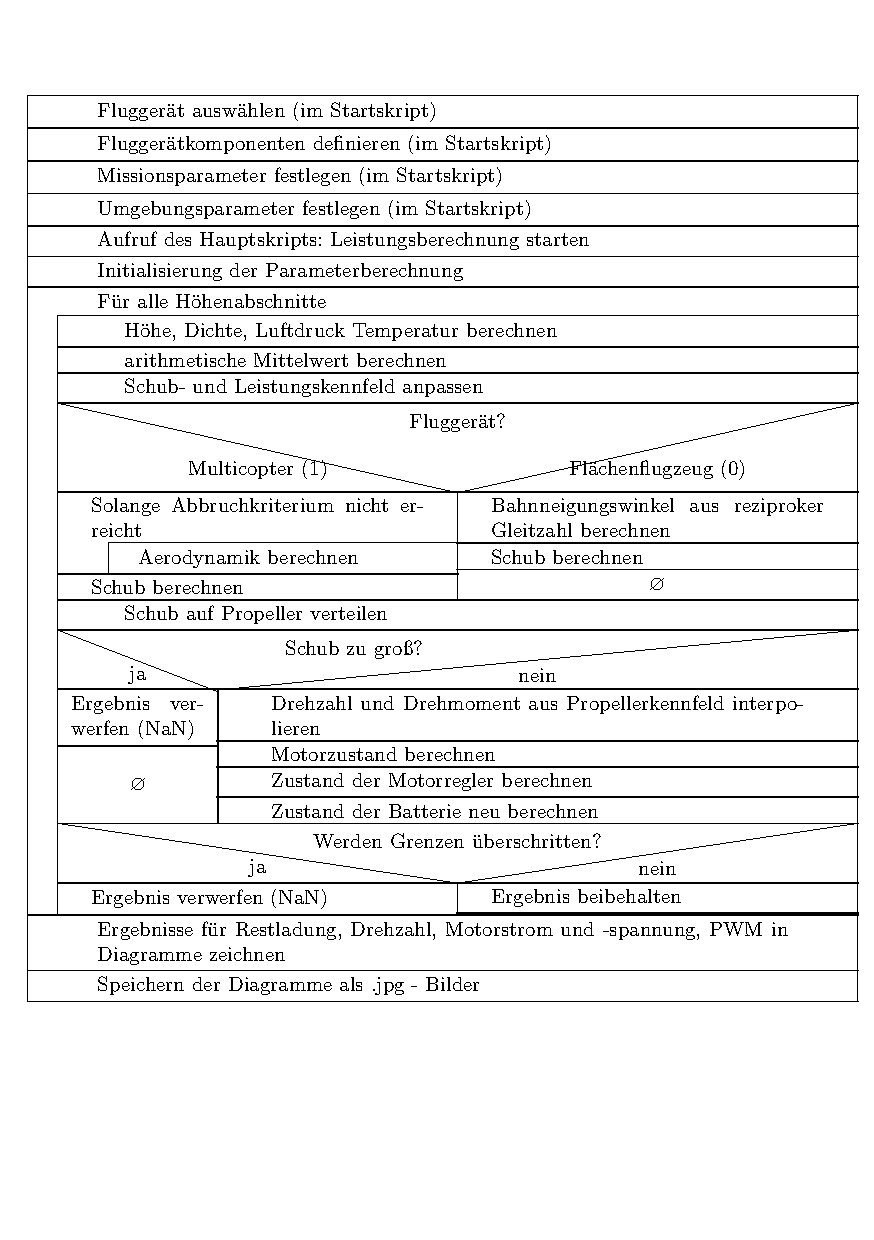
\includegraphics{Struktogramm/Struktogramm.pdf}
%	\caption{Struktogramm des MATLAB-Skripts}
%	\label{abb:struktogramm}
%\end{figure}


\section{Leistungsberechnung}
\label{sec:leistungsberechnung}


\subsection{Veränderung der Umgebungsparameter mit der Höhe}
Für Leistungsuntersuchung wird die Internationale Standardatmosphäre vorausgesetzt. Hiernach ist der Temperaturkoeffizient bis zur Tropopause
\begin{equation}
	\frac{dT}{dH} = -0,0065\frac{K}{m}
\end{equation}
und danach in der unteren Stratosphäre bis zu einer Höhe von \SI{20000}{m}
\begin{equation}
	\frac{dT}{dH} = 0.
\end{equation}
Entsprechend kann der Verlauf der Temperatur, des Druckes und der Dichte von einer Höhe ab \SI{0}{m} bis zur Tropopause (\SI{11000}{m}mit
\begin{equation}
	T_{0-11} = T_0 - \frac{dT}{dH}\cdot H,
\end{equation}
\begin{equation}
	p_{0-11} = p_0\cdot [1-0,0065\frac{K}{m}\cdot \frac{H}{T_0}]^{5,256},
\end{equation}
\begin{equation}
	\rho_{0-11} = \rho_0 \cdot [1-\frac{dT}{dH}\cdot \frac{H}{T_0}]^{4,256}
\end{equation}
beschrieben werden. Ab \SI{11000}{m} ist der Verlauf von Druck und Dichte durch die Gleichungen
\begin{equation}
	p = p_{11}\cdot e^{\frac{g}{R\cdot T_{11}}\cdot (H-H_{11})},
\end{equation} 
\begin{equation}
	\rho = \rho_{11}\cdot e^{\frac{g}{R\cdot T_{11}}\cdot (H-H_{11})}
\end{equation}
gegeben.
Um den Einfluss der Flughöhe in der Leistungsberechnung festzuhalten, werden für jedes Höhenintervall die Umgebungsparameter an den oberen und unteren Intervallgrenzen berechnet. Durch Bildung des arithmetischen Mittelwertes ergeben sich daraus durchschnittliche Parameter für den jeweiligen Höhenabschnitt.  

\subsection{Schub berechnen}
\subsubsection{Multicopter}
Der Schub des Multicopters setzt sich zusammen aus dem zu kompensierenden Gewicht und dem Luftwiderstand durch eine Fluggeschwindigkeit. Dazu kommt noch indirekt der ebenfalls zu kompensierende Seitenwind. Innerhalb eines iterativen, aerodynamischen Modells wird der Schub berechnet. Hierbei sind der Auftriebs- und Widerstandsbeiwert Funktionen des modifizierten Anstellewinkels \ensuremath{\alpha_M} (der Schiebewinkel gibt lediglich die Himmelsrichtung der resultierenden Kraft an, welche in diesem Bericht keine Rolle spielt). Die Idee des Aerodynamischen Modells entstammt aus \textcolor{red}{Beyer,Y.2016b}. 
Die Gesamtmasse des Multicopters setzt sich aus der Masse des Rahmens, der Masse der Batterie, der Masse der Motoren und der Nutzlast
\begin{equation}
	m = m_{copter}+m_{Bat}+m_{Mot}\cdot n_{Prop}+m_{Nutz}
\end{equation}
zusammen.
Die absolute Fluggeschwindigkeit setzt sich zusammen aus Seitenwindgeschwindigkeit und Bahngeschwindigkeit
\begin{equation}
	V_A = \sqrt{(u_{Kg} + u_{Wg})^2+w_{Kg}}
\end{equation}
mit
\begin{equation}
	\begin{pmatrix} u_{Kg} \\ w_{Kg} \end{pmatrix} = \begin{pmatrix}
	\cos\gamma \\ -sin{\gamma}	\end{pmatrix} \cdot V_{kg}.
\end{equation}
Die am Multicopter angreifenden Kräfte werden in Abbildung(einfügen) dargestellt. 
\begin{center}

\includegraphics[scale=0.2]{images/Coming-Soon.jpg}
\end{center}
Für die spätere Koordinatentransformation wird der Windanstellwinkel
\begin{equation}
	\gamma_a = \arctan \Big(\frac{-w_{Kg}}{u_{Kg}+u_{Wg}}\Big)
\end{equation}
berechnet.
Die iterative Berechnung des modifizierten Anstellwinkels 
\begin{equation}
	\alpha_M = \Theta '-\gamma_a
\end{equation} 
beginnt mit dem Startwert für den Steigungswinkel \ensuremath{\Theta_0'=0}.

Im Anschluss werden die aerodynamischen Beiwerte 
\begin{equation}
	c_W = \frac{c_{W,copter,oben}-c_{W,copter,seitlich}}{2}\cdot \cos(2\cdot \alpha_M)+\frac{c_{W,copter,oben}+c_{W,copter,seitlich}}{2}
\end{equation} und 
\begin{equation}
	c_A = c_{A,max}\cdot sin(2\cdot \alpha_M)
\end{equation}
berechnet. Auf diese folgt die Berechnung der aerodynamischen Kräfte
\begin{equation}
	W = c_W\cdot \frac{\rho}{2}\cdot A_{copter,oben}\cdot V_A^2,
\end{equation}
\begin{equation}
	A = c_A\cdot \frac{\rho}{2}\cdot A_{copter,oben}\cdot V_A^2.
\end{equation}
Die aerodynamischen Kräfte werden dann vom aerodynamischen Koordinatensystem in das geodätische Koordinatensystem transformiert:
\begin{equation}
	\begin{pmatrix} X^A \\ Y^A \\Z^A \end{pmatrix}_g = \begin{pmatrix} \cos\gamma_a & 0 & -\sin\gamma_a \\ 0 & 1 & 0 \\ \sin\gamma_a & 0 & \cos\gamma_a \end{pmatrix}^T\cdot \begin{pmatrix} -W \\ 0 \\ -A \end{pmatrix}_a = \begin{pmatrix} -W\cdot\cos\gamma_a-A\cdot\sin\gamma_a \\ 0 \\ W\cdot\sin\gamma_a-A\cdot\cos\gamma_a \end{pmatrix}_g.
\end{equation}
Der Neigungswinkel kann aus dem Kräftegleichgewicht
\begin{equation}
	\Theta_i' = -\arctan\Big(\frac{-X_g^A}{Z_g^A + m\cdot g}\Big), \qquad i =1,2,3,\dots
\end{equation}
neu berechnet werden und geht als Startwert in den nächsten Iterationsschritt ein. Die Iteration erfolgt solange bis das Abbruchkriterium
\begin{equation}
	\Delta\Theta' = \Theta_i-\Theta_{i-1}\stackrel{!}{<}0,001^{\circ}
\end{equation}
erfüllt wird. 
Ist das Abbruchkriterium erreicht, kann der erforderliche Schub mit dem Satz des Pythagoras aus den Kraftanteilen in \(x_g-\) und \(z_g-\)Richtung
\begin{equation}
	S = \sqrt{{X_g}^2+(Z_g^A+m\cdot g)^2}
\end{equation}
bestimmt werden.
Für den Fall, dass der errechnete Schub größer als der zur Verfügung stehende Schub ist, wird das Ergebnis verworfen und als \texttt{NaN} (Not a Number) gespeichert.

\subsubsection{Flächenflugzeug}
Der Schub für ein Flächenflugzeug berechnet sich aus der Kompensation des Widerstandes und des Anteils der zu kompensierenden Gewichtskraft. Analog zum Multicopter setzt sich die Gesamtmasse des Flächenflugzeugs aus der Summe aller Komponenten zusammen
\begin{equation}
	m = m_{Flugzeug}+m_{Bat}+m_{Mot}\cdot n_{Prop}+m_{Nutz}.
\end{equation}
Aus dem Kräftegleichgewicht aller angreifenden Kräfte am System können folgende Beziehungen 
\begin{equation}
	F = W + \sin\gamma\cdot G, \label{eq:widerstandsgleichung}
\end{equation}
\begin{equation}
	A = \cos\gamma G \label{eq:auftriebsgleichung}
\end{equation}
entnommen werden.
Mit
\begin{equation}
	E = \frac{A}{W}
\end{equation}
bzw.
\begin{equation}
	\varepsilon = \frac{W}{A} = \frac{c_W}{c_A}
\end{equation} 
können die Gleichungen \eqref{eq:widerstandsgleichung} und \eqref{eq:auftriebsgleichung} umgeformt werden zu
\begin{equation}
	F = G\cdot\cos\gamma\cdot\Big(\frac{1}{E}+\tan\gamma\Big) = G\cdot(\sin\gamma+\varepsilon\cdot\cos\gamma).
\end{equation}



\subsection{Drehzahl und Drehmoment aus Propellerkennfeld interpolieren}
In der Propellerdatenbank vom Propellerhersteller APC sind zu jedem Propeller dieser Marke die Kennfelder aus Standschubversuchen aufgeführt. Die Art der Aufführung lässt allerdings keine Interpolation der Drehzahl bzw. des Drehmomentes in Abhängigkeit des Schubes und der absoluten Fluggeschwindigkeit zu. Aus diesem Grund muss das Kennfeld auf äquidistante Geschwindigkeitsabstände transformiert werden. Dazu wird ein Geschwindigkeitsvektor mit Abständen von \SI{1}{m/s} gebildet. Die Funktion \texttt{Propeller\_map} (entommen aus Beyer, Y. (2016)) interpoliert danach das Schub- und Leistungskennfeld neu über der Geschwindigkeit und Drehzahl. Mit dem zuvor berechneten Schub und der absoluten Fluggeschwindikeit kann schließlich mit der Funktion \texttt{Propeller} die Drehzahl und das Drehmoment mittels linearer Interpolation ermittelt werden.
Die Kennfelder wurden in Versuchen ermittelt, die keine ändernde Dichte berücksichtigen. Um den Einfluss der sich verringernden Dicht mit zunehmender Flughöhe trotzdem zu beachten, müssen die Kennfelder angepasst werden. Gemäß der Strahltheorie setzt sich der Schub aus dem Massenstrom und der Geschwindigkeit im voll ausgebildeten Abstromzylinder 
\begin{equation}
	T =  \dot{m}\cdot v_{\infty} = \rho\cdot A_{Propeller}\cdot v_i\cdot v_{\infty}
\end{equation}
zusammen. Unter der Annahme vernachlässigbar kleiner Differenzen von  induzierten Geschwindigkeiten $v_i$ und Geschwindigkeiten im voll ausgebildeten Abstrom $v_{\infty}$ kann das Schubfeld des Propellers an den Höheneinfluss 
\begin{equation}
	\frac{T_1}{T_2} = \frac{\rho_1}{\rho_2}
\end{equation}
angepasst werden.


\subsection{Motorzustand berechnen}
Mit dem Drehmoment und der Drehzahl des Propellers berechnet sich der Motorzustand, genauer der Motorstrom und die Motorspannung. Dies erfolgt nach einem einfachen Motormodell \textcolor{red}{Drela 2007}.
Der Motorstrom berechnet sich aus 
\begin{equation}
	I_{Mot} = Q\cdot K_v + I_0.
\end{equation}
Mit dem Strom ergibt sich die Spannung zu
\begin{equation}
	U_{Mot} = \frac{\omega}{K_v} + R_i\cdot I_{Mot}.
\end{equation}


\subsection{Zustand der Motorregler}
Das Modell der Wirkungsgradsberechnung von bürstenlosen Gleichstrom-Motorreglern (Electronic Speed Control (ESC)) stammt aus \textcolor{red}{Lubrano 2016} und wird auch in \textcolor{red}{Beyer 2016b} verwendet. Hiernach berechnet sich der Wirkungsgrad 
\begin{equation}
\eta_{ESC} = \begin{cases} 
0,7\cdot PWM + 0,50 & wenn \qquad 0 < PWM \leq 0,5 \\ 
0,2\cdot PWM + 0,75 & wenn \qquad 0,5 < PWM \leq 1 \\ 
undefiniert & sonst 
\end{cases}
\end{equation} 
mit der Pulsweitenmodulation (PWM) 
\begin{equation}
	PWM = \frac{U_{mot}}{U_{Bat}},
\end{equation}
die sich aus dem Spannungsverhältnis des ESCs zusammensetzt.


\subsection{Batteriezustand}
Die wesentliche Zustandsgröße der Batterie ist der Entladestrom \ensuremath{I_{Bat}}. Dieser setzt sich aus den einzelnen Motorströmen zusammen und zusätzlich dem Wirkungsgrad der Pulsweitenmodulation.
\begin{equation}
	I_{Bat} = I_{Mot}\cdot \frac{PWM}{\eta_{PWM}}\cdot n_{Prop}.
\end{equation}
\begin{equation}
	\dot{C} = \frac{I_{Bat}[A]}{C_{Bat}[A]}\cdot n_{Prop}
\end{equation}
\begin{equation}
	C_{Bat,Peukert} = C_{Bat}\cdot (\frac{1}{\dot{C}})^{P_{Bat}-1} 
	\qquad mit P_{Bat} \geq 1,
\end{equation}
\begin{equation}
	\Delta C_{Bat,i} = I_{Bat}\cdot t_{Flug} + \Delta C_{Bat,i-1} 
	\qquad mit \Delta C_{Bat,0} = 0.
\end{equation}
\begin{equation}
	Restladung_i[\%] = \frac{C_{bat,Peukert}-\Delta C_{Bat,i}}{C_{Bat,Peukert}}\cdot 100\%
\end{equation}


Bei Batterien, hier vor allem Li-Ion und Li-Po, ist die Batteriespannung abhängig von der Entladerate und der Zeit. Hierzu hat \textcolor{red}{Tremblay Blub} ein einfaches Modell aufgestellt, in welchem dieser Zusammenhang berücksichtigt wird \textcolor{red}{Vgl. Abb. Blub}. 
\begin{center}
	
\includegraphics[scale=0.2]{images/Coming-Soon.jpg}
\end{center}
Die Batteriespannung errechnet sich nach 
\begin{equation}
	V_{bat} = E_0-K\cdot\frac{Q}{Q-\int_{}^{} I_{bat} dt}\cdot\int_{}^{} I_{bat} dt - R\cdot I_{bat}+A\cdot e^{-3\cdot\int_{}^{} I_{bat} dt}-K\cdot\frac{Q}{Q-\int_{}^{} I_{bat} dt}\cdot i^* .
\end{equation}
Danach können die unbekannten Batterieparameter einfach mit 3 diskreten Punkten nach folgendem Schema
\begin{equation}
	\begin{pmatrix} E_0 \\ A \\ K \end{pmatrix} = A^{-1}\cdot \begin{pmatrix}
	V_{full}+R\cdot I_{bat} \\ V_{exp}+R\cdot I_{bat} \\ V_{nom}+R\cdot i \end{pmatrix}
\end{equation}
mit
\begin{equation}
	A = \begin{pmatrix}
	1 & 1 & 0 \\ 1 & e^{-3} & -\frac{Q\cdot (Q_{exp}+I_{bat})}{Q-Q_{exp}} \\ 1 & e^{-3\cdot\frac{Q_{nom}}{Q_{exp}}} & -\frac{Q\cdot (Q_{exp}+I_{bat})}{Q-Q_{exp}}
	\end{pmatrix}
\end{equation}
bestimmt werden.
Um eine möglichst einfache Handhabung zu gewährleisten und eine Batteriezellen unabhängig vom Hersteller, der Kapazität und der maximalen Entladerate verwenden zu können, ist die Erstellung einer Normzelle von Interesse. Aus \textcolor{red}{Beyer2016a Blub} existiert bereits eine Datenbank mit mehreren Batterien unterschiedlicher Herstellern, in der alle benötigten Daten zur Erstellung dieser Zelle vorhanden sind. Benötigt werden folgende Punkte: 
\begin{itemize}
	\item die Kapazität Q
	\item die $Q_{exp} Q_{nom}, V_{full}, V_{exp}, V_{nom}$, R und i
\end{itemize}
Hierbei sind schon $V_{full}, V_{exp} und V_{nom}$ auf eine Zelle normiert, allerdings die anderen Parameter nicht. Aus diesem Grund werden alle übrigen Parameter mit \SI{1}{Ah} normiert und der arithmetische Mittelwert über alle Batterien gebildet. Der Entladestrom entspricht dabei dem 1/100 der Batteriekapazität also \SI{1}{Ah}. Für den auf \SI{1}{Ah} genormten Innenwiderstand lässt sich ein hyperbolischer Verlauf über der Kapazität feststellen. Mittels einer Regression kann der Innenwiderstand für eine Zelle mit \SI{1}{Ah} ermittelt werden. 
Der Vergleich der berechneten Normzelle mit originalen Batterien teils starke Abweichungen von über 100\% von der ursprünglichen Batteriezelle. Zusätzlich wird der Einfluss der C-Rate auf diese Abweichungen mit berücksichtigt. Dabei kam heraus, dass gewisse Batterien signifikant von der angenäherten Zelle abweichen (z.B. Batterienummer 14,30,40 und 63). Diese wiesen deutliche Abweichungen von der mittleren Abweichung aller Zellen auf. Aus diesem Grund sind diese Batterien aus der Betrachtung entfernt und die Mittelwerte neu berechnet worden.




\begin{itemize}
	\item Es ist eine Datenbank von Elektromodellflug vorhanden, in der die lastabhängige Entladekurve verschiedener Batterien unterschiedlicher Hersteller und unterschiedlichen Kapazitäten, Massen etc. dargestellt sind
	\item Ziel ist, unabhängig vom Hersteller, der Kapazität, der Masse, der max. Dauerentladerate, etc. ein Batteriemodell aufzustellen für eine Zelle
	\item Dazu muss eine Normzelle hergestellt werden <-- anders formulieren
	\item Enstsprechung wurden alle Batterien der Datenbank auf eine \SI{1}{Ah} normiert.
	\item dazu arithmetischer Mittelwert von Q, Qexp und Qnom bezogen auf eine Ah, die Angaben V, Vexp,Vfull waren entsprechend genormt, nur Mittelwert berechnen
	\item Der Strom i ist auf 1/100 der Kapazität oder Entladerate bezogen
	\item für Innenwiderstand ist auch genormt auf 1Ah. Es lässt sich ein hyperbolischer Verlauf der des Widerstandes über der Kapazität feststellen.
	\item --> Regression durch die Punkte legen mit lsqcurvefit. 
	\item Vergleich aufgestellten Modells zu Originalzellen. 
	\item Feststellung der Abweichungen des Modells von der Originalzelle, dazu Bestimmung starker Diskrepanzen einzelner Zellen von der Normzelle und Bestimmung einer Tendenz der Abweichung. 
	\item Korrektur dieser durch Errechnung der Standardabweichung und Festlegung des Konfidenzintervalls  
\end{itemize}


\subsection{Wirkungsgrad über das Gesamtsystem}
Zur Berechnung des Wirkungsgrads kann das Verhältnis der Leistung, die in Schub gewandelt wird zu der Leistung, die der Batterie entzogen wird, herangezogen werden
\begin{equation}
	\eta_{ges} = \frac{P_{Strahl}}{P_{Bat}}.
\end{equation}
Die Strahlleistung 
\begin{equation}
	P_{Strahl} = T\cdot (v_i + V_c)
\end{equation}
setzt sich aus dem Schub \ensuremath{T}, der induzierten Geschwindigkeit \ensuremath{v_i} und der Steiggeschwindigkeit \ensuremath{V_c} zusammen.
Zur Berechnung der induzierten Geschwindigkeit im Steigflug wird das Newton-Raphson-Verfahren herangezogen. Mit diesem lässt sich innerhalb weniger Iterationsschritte die induzierte Geschwindigkeit im Steigflug ermitteln \textcolor{red}{van der Wall}:
\begin{equation}
	f(v) = v-\mu_z-\frac{{v_h}^2}{\sqrt{\mu^2+v^2}}
\end{equation}
\begin{equation}
	f'(v) = 1 + v\cdot\frac{{v_h}^2}{\sqrt{\mu^2+v^2}^3}
\end{equation}
\begin{equation}
	v_{n+1} = v_n - \frac{f(v_n)}{f'(v_n)}\qquad n = 0,1,2,\dots
\end{equation}
An dieser Stelle sei angemerkt, dass van der Wall mit dimensionslosen Durchflussgraden \ensuremath{\lambda} rechnet. In dieser Arbeit wird aber mit den dimensionsbehafteten Geschwindigkeiten gerechnet.
Der Startwert der Iteration ist die induzierte Geschwindigkeit im Schwebeflug
\begin{equation}
	v_h = \sqrt{\frac{m\cdot g}{2\cdot\rho\cdot A_{Rotor}\cdot n_{Prop}}}.
\end{equation}
Die der Batterie entzogenen Leistung
\begin{equation}
	P_{Bat} = U_{Bat}\cdot I_{Bat}
\end{equation}
ist das Produkt aus der Batteriespannung und -strom.


\subsection{Werden Grenzen überschritten?}
Für den Fall, dass technisch und aerodynamisch unmögliche Flugzustände erreicht werden, sind folgende technische und aerodynamische Grenzen festgelegt:
\begin{itemize}
	\item Die Restladung im Steigflug ist kleiner als  Null oder kleiner als eine vorher festgelegte, minimale Restkapazität (Kapazität der Batterie reicht nicht aus oder zu hohe Flugzeit)
	\item Die Motorspannung ist größer als die nominelle Spannung der Batterie (zu hohe Winkelgeschwindigkeit im Steigflug erforderlich)
	\item Die Motorspannung ist kleiner/gleich Null (zu schneller Sinkflug, diese Grenze kann in einem Steigflug nicht erreicht werden, ist der Vollständigkeit halbe trotzdem mit berücksichtigt)
	\item Die C-Rate ist größer als die maximal zulässige C-Rate der Batterie (Batterieentladestrom ist höher als zulässig)
	\item Der Motorstrom ist höher als der maximal zulässige Dauerstrom des Motors unter Last (zu hohes Drehmoment gefordert)
	\item Der lokale Anstellwinkel überschreitet den festgelegten Grenzwert von \ensuremath{\alpha_{max}}(Strömungsabriss)
	\item Die Blattspitzengeschwindigkeit überschreitet \ensuremath{M_{tip}=1}(transsonische Strömung)
\end{itemize}

\section{Vernachlässigungen und Vereinfachungen}
\label{sec:vernachlaessigungen_vereinfachungen}

\subsection{Einschränkungen}
Für die Leistungsberechnung sind mehrere Vernachlässigungen vorzunehmen. Zuerst wurden keinerlei dynamische Effekte und Verhalten berücksichtigt. Dies beinhaltet translatorische Beschleunigungen des Multicopters, rotatorische Beschleunigungen der Rotoren zum Störausgleich sowie und rotatorische Beschleunigungen des Multicopters durch Ungenauigkeiten des Lagereglers. Das gleiche gilt für das Flächenflugzeug. 
Die Störgrößen, in diesem Fall vor allem der laterale Seitenwind, werden als statisch und konstant vorausgesetzt. Hierbei werden jegliche Veränderungen des Windes und Böen mit der Höhe vernachlässigt. Auf- und Abwinde entziehen sich auch der Betrachtung. Hinzu kommt die Vernachlässigung der Totzeit des Reglers. 
Weiterhin nicht berücksichtigt bleiben Reynoldszahl- und Machzahleffekte. Transonische Strömung unterhalb einer Blattspitzengeschwindigkeit von \ensuremath{M_{tip}=1} kann aus diesem Grund nicht ausgeschlossen werden.
Die ganze Leistung der Batterie geht in diesem Modell ausschließlich in die Schuberzeugung. Das heißt, dass die Regler und sonstige elektrische Komponenten keinen zusätzlichen Strom verbrauchen.
Das Flächenflugzeug wird in dem Programm als eine Punktmasse ohne Abmaße betrachtet. Um eine möglichst allgemeine Dimensionierung eines Flugsystems mit fixed wings zu ermöglichen wird sich hier jeglicher genauerer Beschreibungen des Systems verwehrt. So wird auf Kennzahlen wie die Streckung, die Flügelfläche oder z.B. Auftriebs- und Widerstandsbeiwerten verzichtet. Dies zieht eine derartige Betrachtung des Systems mit sich, dass nur der Einfluss von Gleitzahl, Motorisierung und anderen Einflussfaktoren betrachtet werden. Eine exakte Auslegung kann deshalb nur im Anschluss vorgenommen werden. Diese Vereinfachungen müssen in der Auswertung berücksichtigt werden.
%\begin{itemize}
%	\item einfaches Motormodell, i.e. Abweichungen
%	\item Frage nach der Genauigkeit der Kennfelder
%	\item lineare Interpolation und generell Interpolation, d.h. Abweichungen t%treten auf
%	\item vereinfachende Annahmen einer Normatmosphäre und eines konstanten %Windprofils über der Höhe
%	\item keine Berücksichtigung dynamischer Effekte wie Beschleunigung des %Systems, Drehträgheiten, Beschleunigungen durch Störausgleiche etc.
%	\item vereinfachende Aerodynamik, keine Berücksichtigung von Reynoldszahleffekten. Machzahleffekte nur angenähert. Effekte können beim Propeller nicht ausgeschlossen werden
%	\item weitere Leistung zum Betrieb des Reglers oder anderer elektrischer Systeme wurde nicht berücksichtigt 
%\end{itemize}

\subsection{Vereinfachungen}
\subsubsection{Schub}
Der Schub wird innerhalb eines sehr einfachen Modells berechnet. Das gilt sowohl für den Multicopter als auch für das Flächenflugzeug. Der Multicopter ist als eine Art Rotationsellipsoid und das Flächenflugzeug als Punktmasse vereinfacht

\subsubsection{Propeller und Kennfeld}
Bei der Transformation der Propellerkennfelder auf äquidistante Geschwindigkeitsabstände ist der Bereich von \SI{-10}{m/s} bis \SI{0}{m/s} extrapoliert. Das reale Verhalten der Propeller kann folglich von dem errechneten abweichen. Weiterhin beziehen sich alle Auslegungen auf die Datenbank von APC. 
Die Modellierung eines Propellers mit gleichem Durchmesser und gleicher Steigung eines anderen Herstellers kann aus diesem Grund abweichen. Gründe dafür können eine unterschiedliche Profilierung, Verwindung oder Profiltiefenverteilung sein. 

\subsubsection{Motor}
Jeglicher Einfluss der Temperatur auf die Leistung des Motors bleibt in dem einfachen Motormodell unberücksichtigt. Außerdem werden der Motorstrom und der der Innenwiderstand als konstant angenommen.

\subsubsection{Motorregler}
Für den Motorregler wurde ein sehr einfaches Modell verwendet, in dem der Wirkungsgrad ausschließlich eine Funktion der PWM ist.

\subsubsection{Batterie}
Die Berechnung der Batterie vernachlässigt zwei wichtige Einflussfaktoren. Das ist der Temperatureinfluss und der Einfluss der Alterung auf die Kapazität. Dies kann jedoch durch eine Anpassung der Peukert-Konstante kompensiert werden. Weiterhin wird ein Einbruch der Batteriespannung in Abhängigkeit der Entladerate nicht berücksichtigt.

\subsubsection{Wirkungsgrad}
Die Berechnung der Strahlleistung beruht auf der Berechnung der induzierten Geschwindigkeit innerhalb der Strahltheorie. Hier wird ein idealer Rotor zugrunde gelegt.
Beruhend auf dieser Annahme bleiben viele Effekte wie Blattspitzeffekte an der Rotorblattspitze und im Bereich der Rotorblattaufhängung, Strömungsablösungen, Blattwirbelinteraktionen usw. unberücksichtigt.  Zudem wird eine über den Radius konstante induzierte Geschwindigkeit in der Rotorebene angenommen. Dies ist im Vorwärtsflug und bei Schräganströmung zu relativieren \cite{Wall.2015}.
%\begin{itemize}
%	\item Schub: sehr einfaches aerodynamisches Modell
%	\item Kennfeld: Kennfelder einfach angepasst, Kennfelder extrapoliert, Kennfelder nicht validiert, 
%	\item Motor: Vernachlässigung Motorerwärmung, 
%	\item Motorregler: einfaches Modell, nur abhängig von der PWM
%	\item Batterie: Temperatur komplett vernachlässigt, kann großen Einfluss haben auf Kapazität, neue Batterie angenommen, keine Berücksichtigung von Alterseffekten
%	\item Wirkungsgrad nach Strahltheorie, Vorraussetzung eines idealen Rotors und vernachlässigung anderer Verluste wie ungleichförmige Geschwindigkeitsverteilung, Blattspitzeneffekte etc.
%	\item energiedichte nur geschätzt
%\end{itemize}
    \chapter{Nachbildung des Quadrocopterfluges in Russland}
\label{chap:nachbildung_des_quadrocopter}

\section{Komponenten des Quadrocopters}
\label{sec:komponenten}

\section{Nachbildung im Programm}
\label{sec:nachbildung_im_programm}

\section{Ergebnisse}
\label{sec:ergebnisse_quadrocopter}

    \chapter{Vergleich eines Flächenflugzeugs mit dem Quadrocopter}
\label{chap:vergleich}
Jedes Luftfahrzeugkonzept entzieht sich einem direkten Vergleich mit einem Luftfahrzeug einer anderen Art. So weist jedes Fluggerät in seiner Gattung spezifische Vorteile auf wie der Start auf der Stelle und das Hovern in der Luft für Multicopter oder der Gleitflug für Flächenflugzeuge. Die jeweilige Auslegung beider führt zu unterschiedlichen Designs was die Propeller, die Motorleistung und das -gewicht, die Größe, das Gesamtgewicht etc. betrifft. Aus diesem Grund müssen Kriterien für eine Vergleichbarkeit vorgeschrieben werden. Hierfür wird das Design des Multicopters auf das aus \cite{Anderson.2018} festgelegt, welches genauer in Kapitel \ref{sec:komponenten} beschrieben ist. Da die Flugleistungen von \cite{Anderson.2018} bekannt sind und der Quadrocopter durchaus schon im Rahmen der Anforderungen für diese Mission als optimiert betrachtet werden kann, bedarf es an dieser Stelle einer Untersuchung des Flächenflugzeuges. Dazu wird das Flächenflugzeug auf Parameter fixiert, mit denen es bereits sehr hoch aufsteigen kann. Zur Untersuchung und Vergleichbarkeit werden die Gesamtmassen beider Fluggeräte gleichgesetzt \ensuremath{m_{ges,Quadrocopter} = m_{ges,Flächenflugzeug}}. Dabei setzt sich die Masse der Flächenflugzeugbatterie   
\begin{equation}
	m_{Bat,Fl} = m_{Bat,Quad} + (m_{Mot,Quad}\cdot n_{Prop,Quad} - m_{Mot,Fl}\cdot n_{Prop,Fl}) - (1-f_P)\cdot m_{Quad}  
\end{equation}
in Bezug auf bereits gewählte Massen und auf den Quadrocopter zusammen. Der Faktor \ensuremath{f_P} kann als Penalty-Faktor verstanden werden. Dieser verringert zusätzlich die Batteriemasse, wenn das Strukturgewicht des Flächenflugzeugs das des Quadrocopters überschreitet
\begin{equation}
	f_P = \frac{m_{Flugzeug}}{m_{Quad}} \eqend{.}
	\label{eq:penalty}
\end{equation} 
Für eine erste Betrachtung wird der Penalty-Faktor auf 1 gesetzt. Dies entspricht einer optimistischen Einschätzung. Im Anschluss werden die Parameter in näherer Umgebung der ersten festgesetzten Werte variiert. Dadurch kann der Einfluss auf das Leistungsverhalten und die Richtung der möglichen Optimierung bestimmt werden. Diese erste, einfache Untersuchung ist nur eine sehr oberflächliche, weil jeder Parameter nur einzeln und unabhängig von den anderen untersucht wird. Jegliche Kombinationen von Einflüssen wie der Einfluss der Masse auf die Steiggeschwindigkeit oder vergleichbare Beziehungen werden vernachlässigt. Im Hinblick auf diese erste, kleine Optimierung ist der Kostenfaktor die maximal erreichbare Höhe beider Fluggeräte. Je nachdem welches der beiden Fluggeräte effektiver und effizienter eine maximale Flughöhe erreicht, wird es weiter untersucht und anschließend optimiert.  

\section{Einfluss der Steiggeschwindigkeit auf den Quadrocopterflug}
Bevor ein Vergleich zwischen dem Flächenflugzeug und dem Quadrocopter aus Kap. \ref{chap:chap:nachbildung_des_quadrocopter} durchgeführt werden kann, muss noch die Steiggeschwindigkeit für den Quadrocopter optimiert werden. \\
Für das Flächenflugzeug werden für jeden Höhenschritt, wie bereits in Abschn. \ref{subsubsec:schub_flaechenflzg} dargelegt, der Bahnneigungswinkel und die Fluggeschwindigkeit optimiert. Dies entspricht einer ersten Optimierung. Dabei wird der Bahnneigungswinkel für jeden Höhenschritt iteriert. Die Fluggeschwindigkeit berechnet sich in Abhängigkeit vom Bahnneigungswinkel (vgl. Gleichung \eqref{eq:eq:geschw_flaechenflugzeug}). Die Auswahl erfolgt anhand der minimalen Energiemenge, die der Batterie für den Höhenschritt entnommen wird. Analog dazu, erfolgt auch die Optimierung der Steiggeschwindigkeit des Quadrocopters (vgl. Anhang \ref{sec:vvar_vorgehen}). \\
Durch die Optimierung der Steiggeschwindigkeit ist ein zusätzlicher Höhengewinn von \SI{1000}{m} im Vergleich zu dem Flug mit konstanter Bahngeschwindigkeit von \SI{10}{m/s} zu vermerken. Bei dem neuen TOC auf \SI{14100}{m} wird allerdings die sogenannte Dienstgipfelhöhe erreicht (genauere Beschreibung in Abschn. \ref{sec:flaechenflugzeug_referenzkonfig} und \ref{subsec:mot_prop_kombi}). Ohne diese Limitierung und bei linearer Extrapolation Restladungskurve könnte der Quadrocopter bei Verwendung eines anderen Propellers eine Höhe von \SI{17000}{m} erreichen. Die Flugleistungen sind nicht durch die Motorleistung begrenzt, sondern durch die Maximaldrehzahl des Propellers. Diese liegt bei \SI{17000}{RPM}. Ein Grund dafür kann in der Festigkeit des Propellers gefunden werden. Nichtsdestotrotz ist ein Flug mit variierbarer Steiggeschwindigkeit signifikant effizienter. Dies macht sich deutlich in der Restladung bemerkbar. Die Abnahme der Restladung ist pro Höhenschritt geringer als in Kap. \ref{sec:ergebnisse_quadrocopter}. Auf \SI{10260}{m} sind noch \SI{40}{\%} Restladung vorhanden. Das entspricht ca. \SI{10}{\%} mehr Restladung in der gleichen Höhe wie in Kap. \ref{chap:nachbildung_des_quadrocopter}. Die Propellerdrehzahl steigt beinahe sofort auf ihr Maximum von \SI{17000}{RPM} an und verbleibt auf diesem Niveau bis zum TOC. Rückwirkend ist damit auch der Motorstrom ab \SI{4000}{m} auf dem Niveau der Batteriespannung und somit die PWM auf \SI{100}{\%}. Der Leistungsüberschuss ist gleich null. Dieser Zustand ist auch durch ein Maximum der Bahngeschwindigkeit gekennzeichnet mit \SI{30}{m/s}. Die Bahngeschwindigkeit ist damit dreimal so hoch wie die vorherigen \SI{10}{m/s}. Der Motorstrom \ensuremath{I_{Mot}} sinkt im Laufe des Fluges immer weiter ab. Da die Drehzahl konstant bleibt, die Dichte aber mit der Höhe abnimmt, sinkt auch das Drehmoment an der Motorwelle und letztlich der Motorstrom (vgl. Gleichung \eqref{eq:motorstrom}). Über den Motorstrom sinkt die Motorspannung ebenfalls leicht ab (vgl. Gleichung \eqref{eq:motorspannung}), weil die Drehzahl auf einem konstanten Niveau bleibt. Während die Batteriespannung von \SI{16}{V} auf \SI{15}{V} durch die Last einbricht, fällt mit der Motorspannung auch die PWM unterhalb von \SI{100}{\%} ab. Die Bahngeschwindigkeit steigt zuerst auf ihr Maximum, sinkt danach aber kontinuierlich auf \SI{0}{m/s}. Somit wird die Dienstgipfelhöhe erreicht. Die Flugzeit kann auf die Bahngeschwindigkeit zurückgeführt werden. Bereits nach \SI{13}{min} und \SI{20}{sec} wird der TOC erreicht. \\
Der Motorregler verzeichnet wenige Verluste durch die hohe PWM und besitzt deshalb einen hohen Wirkungsgrad. Der Propellerwirkungsgrad steigt am Anfang durch den Drehzahlanstieg (vgl. Gleichung \eqref{eq:eta_prop}) und ebenso mit dem Schub und der Bahngeschwindigkeit. Während der Schubüberschuss aufgebraucht ist, sinkt mit der Höhe die Dichte und dementsprechend der Schub. Mit dem Schub sinkt auch die leistungstechnisch mögliche Bahngeschwindigkeit, was einen starken Einbruch im Propellerwirkungsgrad hervorruft.

\begin{figure}[htb!]
\centering
	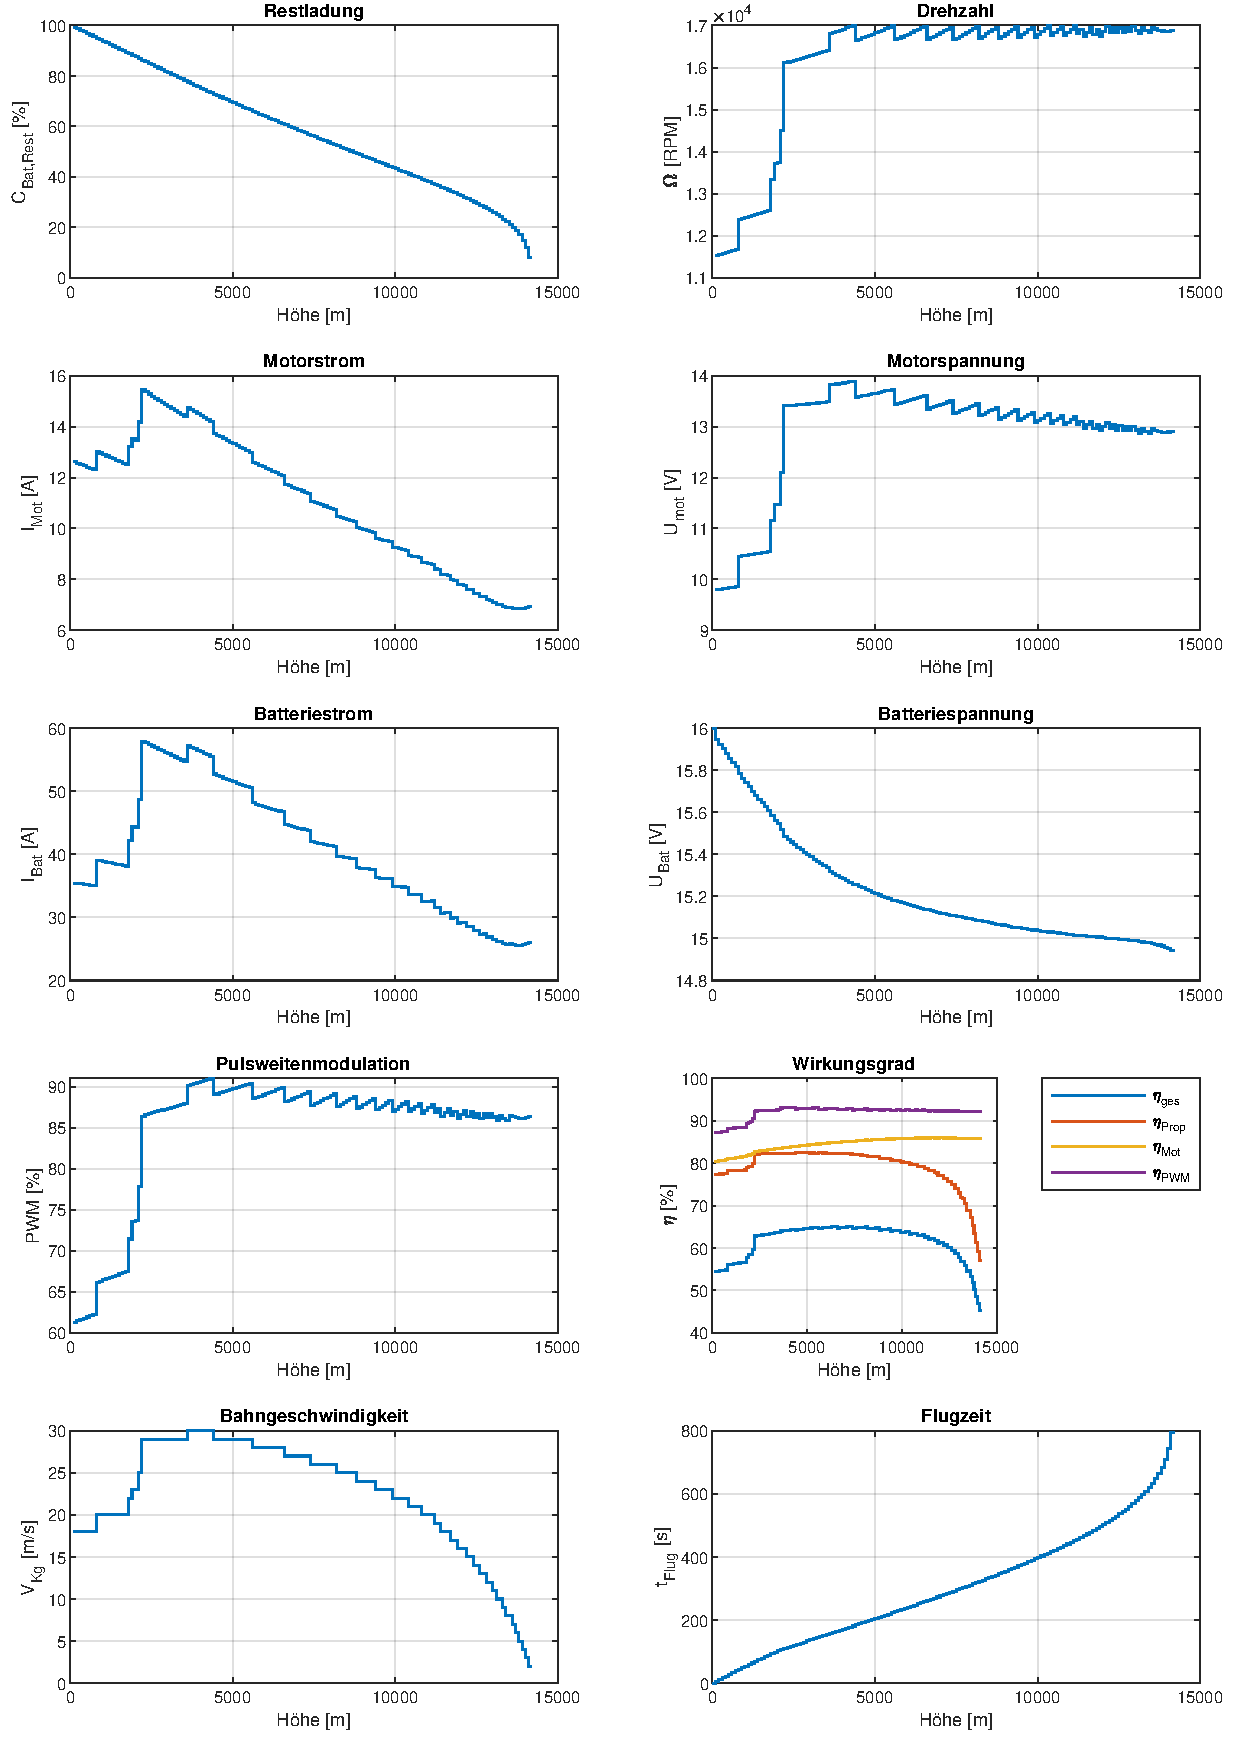
\includegraphics[scale=0.7]{Diagramme/Russland_vvar.pdf}
	\caption{Flugleistungen des Quadrocopter aus \cite{Anderson.2018} mit variabler Steiggeschwindigkeit}
	\label{abb:russland_vvar}
\end{figure}



\section{Flächenflugzeug-Referenzkonfiguration}
\label{sec:flaechenflugzeug_referenzkonfig}
In der Tab. \ref{tab:referenzkonfiguration} sind wichtige Parameter der Referenzkonfiguration für das Flächenflugzeug aufgelistet. Die Werte wurden in ersten Untersuchungen durch Versuche bestimmt. 
\begin{center}
	\captionof{table}{wichtige Parameter der Flächenflugzeug-Referenzkonfiguration}
	\begin{tabular}{l l l} \hline
		Parameter & Variablenname & verwendete Größe \\ \hline
		Leermasse des Flächenflugzeug \ensuremath{m_{Flugzeug}}& \texttt{m\_Flugzeug} & \SI{0,354}{kg} \\ 
		Batteriemasse \ensuremath{m_{Bat}} & \texttt{m\_Bat} & \SI{0,56}{kg} \\
		Motormasse \ensuremath{m_{Mot}}& \texttt{m\_Mot} & \SI{0,106}{kg} \\
		Geschwindigkeitskonstante \ensuremath{K_V} & \texttt{K\_V} & \SI{1390}{RPM/V} \\
		maximaler Dauerstrom \ensuremath{I_{max}} & \texttt{I\_max} & \SI{35}{A} \\
		Propeller & \texttt{prop\_name} & 9x7 \\
		Anzahl Propeller \ensuremath{n_{Prop}} & \texttt{n\_prop} & \SI{1}{} \\
		Auslegungsgleitzahl \ensuremath{E^{\star}} & \texttt{E\_stern} & \SI{4}{} \\
		Auslegungsgeschwindigkeit \ensuremath{V^{\star}} & \texttt{V\_stern} & \SI{100}{km/h} \\
		Gleitzahl \ensuremath{E} & \texttt{E} & \SI{4}{} \\ 
		Anzahl der Batteriezellen \ensuremath{N_{Bat,cell}} & \texttt{N\_bat\_cell} & 6 \\	
		Penalty-Faktor \ensuremath{f_P}	& \texttt{f\_P}	& 1 \\ \hline
	\end{tabular}	
	\label{tab:referenzkonfiguration}
\end{center}
Diese Konfiguration ist die Grundlage aller Untersuchungen, die das Flächenflugzeug betreffen.



\begin{figure}[htb!]
%\centering
	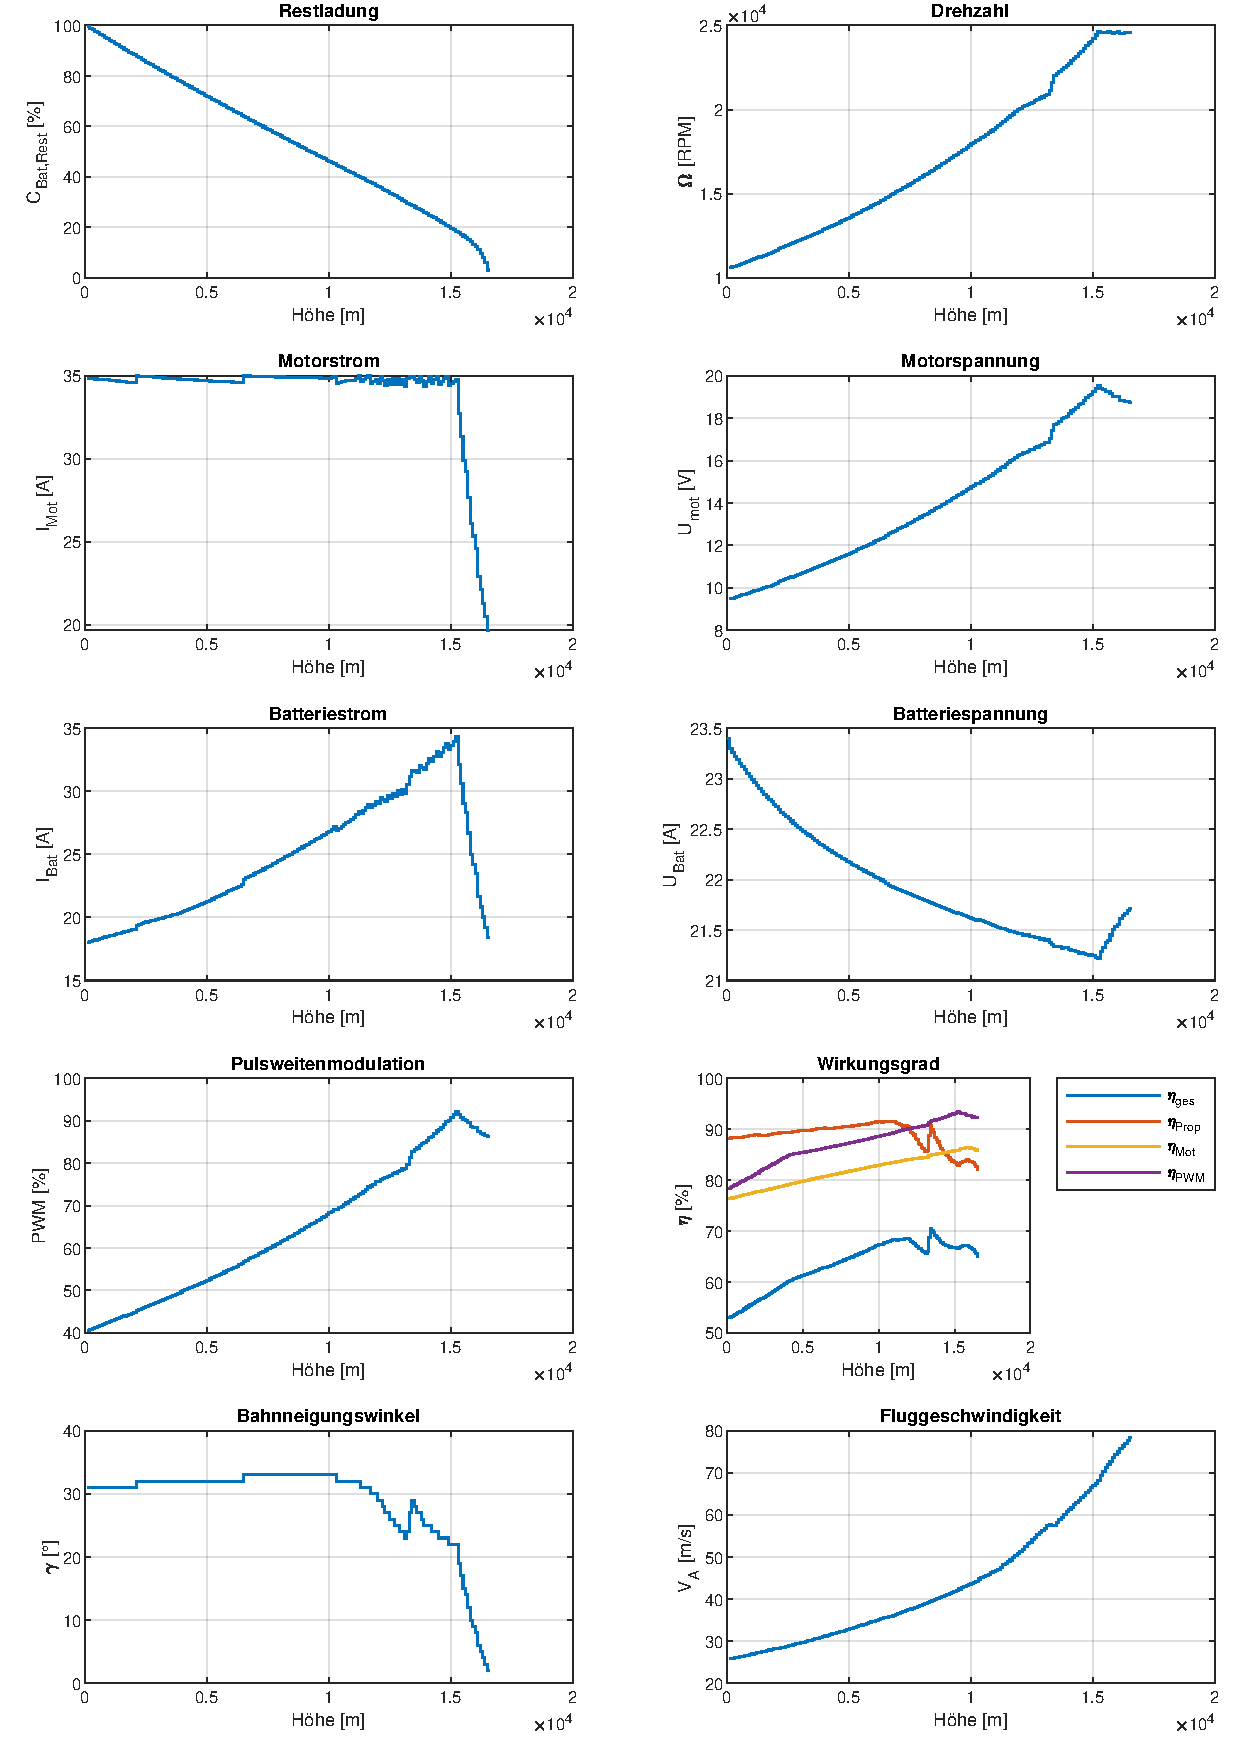
\includegraphics[scale=0.7]{Diagramme/Ausgangskonstellation.pdf}
	\caption{Verlauf der Leistungsparameter über der Höhe für die Flächenflugzeug-Referenzkonfiguration (Tab. \ref{tab:referenzkonfiguration})}
	\label{abb:referenzkonfiguration}
\end{figure}
Die in Tab. \ref{tab:referenzkonfiguration} beschriebene Referenzkonfiguration erreicht bereits eine Flughöhe von \SI{16500}{m}. Der limitierende Parameter für den Aufstieg in noch größere Höhen ist in diesem Fall nicht die Motorleistung, sondern die maximale Propellerdrehzahl (vgl. Abb. \ref{abb:referenzkonfiguration}). Eine weitere Erhöhung der Drehzahl ist in diesem Fall wegen folgender zwei Einflussfaktoren nicht möglich. Zum einen ist die maximale Propellerdrehzahl auf \SI{25000}{RPM} durch das Ende des Kennfeldes begrenzt. Dies ist mit hoher Wahrscheinlichkeit auf die Festigkeit des Propellers zurückzuführen. Bis zu dieser Drehzahl ist ein uneingeschränkter Betrieb des Propellers möglich, ohne das ein strukturelles Versagen des Propellers zu befürchten ist. Ab einer höheren Drehzahl kann ein sicherer Betrieb nicht mehr gewährleistet werden. Der zweite Einflussfaktor ist die Blattspitzengeschwindigkeit \ensuremath{Ma_{tip}}. Diese erreicht ab \SI{15000}{m} Höhe \ensuremath{Ma_{tip} = 1}. Damit kommt es zu Machzahleffekten und einer relativen Überschallanströmung an der Propellerblattspitze. Die dadurch verursachten zusätzlichen Verluste (z.B. Stoßverluste), Stömungsablösungen, Verminderungen in der Schuberzeugung usw. können nicht in dem einfachen Luftmodell berücksichtigt werden, das dem in Kap. \ref{chap:Programmbeschreibung} erläuterten Programm zur Flugleistungsberechnung zugrunde gelegt wurde. An dieser Stelle können transsonische Effekte, die bereits bei einer relativen Anströmung an der Propellerspitze von \ensuremath{Ma < 1} auftreten können, nicht ausgeschlossen werden. Die Möglichkeiten zur Vermeidung dieser Begrenzung werden in Abschn. \ref{subsec:propeller} beschrieben. \\
Die Limitierung der Flughöhe durch die maximale Propellerdrehzahl stellt eine sogenannte Dienstgipfelhöhe dar. Diese limitiert den Steigflug bereits zu Beginn des Starts auf \SI{16500}{m}. Eine Erhöhung der Motorleistung, der Batteriezellenanzahl oder beispielsweise der Kapazität würde keine weiteren Verbesserungen der Flugleistungen erbringen, da die Begrenzung durch die Propellerdrehzahl für jeden Flug dieselbe ist. Generell ist eine Erhöhung des Leistungsüberschuss (\ensuremath{=} Erhöhung der Leistung) damit nicht zielführend. Ein Steigflug ohne Dienstgipfelhöhe zeichnet sich durch die Limitierung der Flughöhe durch die Restladung aus. Hierbei sinkt diese linear ab bis \SI{0}{\%} Restladung erreicht sind. \\
Das Erreichen der Dienstgipfelhöhe zeichnet sich durch eine Verschlechterung Flugleistungen aus. Die Restkapazität nimmt mit der Höhe linear ab. Ab der Höhe von \SI{15000}{m} wird die maximale Propellerdrehzahl erreicht, sodass sich die Abnahme der Restkapazität erhöht. \\
Der Steigflug bis \SI{15000}{m} ist durch den Betrieb bei maximalem Dauerstrom (\ensuremath{I_{max} = \SI{35}{A}}) gekennzeichnet. Dadurch stellt sich ein optimaler Bahnneigungswinkel von \SI{31}{^\circ} bis \SI{33}{^\circ} ein. Dieser Winkel kann bis zu einer Höhe von \SI{10000}{m} gehalten werden, bevor er zunächst langsam absinkt und ab \SI{15000}{m} steil gegen \SI{0}{^\circ} strebt. Die Fluggeschwindigkeit steigt mit dem Steigwinkel progressiv mit dem Produkt aus \ensuremath{\sqrt{\rho^\star/\rho}} an (vgl. Gleichung \eqref{eq:geschw_flaechenflugzeug}). \\
Zu Beginn des Steigfluges wären größere Steigwinkel effizienter, allerdings werden diese durch den maximalen Motorstrom \ensuremath{I_{max}} begrenzt. Ohne diesen würde der Bahnneigungswinkel beinahe linear absinken. Daraus kann geschlossen werden, dass ein Flug mit maximalem Motorstrom im unteren Höhenbereich am effizientesten ist. Der sägezahnartige Verlauf des Motorstroms hängt mit der gewählten Diskretisierung und dadurch rückwirkend mit der Genauigkeit der Berechnung zusammen. Eine genauere Untersuchung der in den Diagrammen dargestellten Punkte und deren Umgebung würde zu einem glatten Verlauf des Motorstroms bei \ensuremath{I_{max}} führen. Ebenso würden sich die Verläufe aller anderen Leistungsparameter über der Höhe glätten. Gleichzeitig zum konstanten Motorstrom wächst die Motorspannung linear an, bis diese ab \SI{9800}{m} das Niveau der Batteriespannung erreicht. \\
Auch die Propellerdrehzahl weist eine progressive Zunahme auf. Mit der Höhe sinkt die Dichte der Luft entsprechend nach Gleichung \eqref{eq:rho_0_11} und \eqref{eq:dichte_strato}. Zur Erzeugung des gleichen Schubs muss mit der abnehmenden Dichte die Drehzahl steigen, um den Massenstrom durch die Propellerebene und letztendlich den Schub konstant zu halten (vgl. Gleichung \eqref{eq:propellerschub}). Bei konstantem Motorstrom und steigender Propellerdrehzahl nimmt entsprechend auch die Motorspannung zu (vgl. Gleichung \eqref{eq:motorspannung}). \\
Der Verlauf des Batteriestroms steht in direktem Zusammenhang mit dem Motorstrom und der Motorspannung. Dies wird aus Gleichung \eqref{eq:batteriestrom} ersichtlich. Bei einem konstantem Motorstrom ist  \ensuremath{I_{Bat}} nur von \ensuremath{U_{Mot}} abhängig. Daher zeigt sich der gleiche Verlauf wie bei \ensuremath{U_{Mot}}. Ab dem Erreichen der maximalen Propellerdrehzahl nimmt \ensuremath{U_{Mot}} wieder leicht ab und \ensuremath{I_{Bat}} hängt nur noch von \ensuremath{I_{Mot}} ab. Der Verlauf der Drehzahl ist ausschlaggebend für die Motorspannung. Die Batteriespannung bricht durch die Belastung von anfänglichen \SI{23,4}{V} auf \SI{21,2}{V} ein. 
Die PWM steigt mit dem Verlauf der Motorspannung sowie der Batteriespannung an. Ab \SI{15000}{m} erreicht sie ihr Maximum bei \SI{91,5}{\%}. Dies verdeutlicht noch einmal, dass für die Referenzkonfiguration die Motorleistung nicht den die Höhe limitierenden Leistungsparameter darstellt. \\
Ist die maximale Propellerdrehzahl ab \SI{15000}{m} erreicht, fällt der Motorstrom rapide mit der konstanten Drehzahl ab. Da die Drehzahl konstant bleibt bis zum TOC, nimmt das Propellerdrehmoment und damit auch der Motorstrom mit zunehmender Höhe und abnehmender Dichte ab (vgl. \eqref{eq:motorstrom}). Mit sinkendem Motorstrom sinkt auch die Motorspannung  (vgl. Gleichung \eqref{eq:motorspannung}) und schließlich die PWM (vgl. Gleichung \eqref{eq:pwm}). Dieser Effekt wird noch durch den Anstieg der Batteriespannung auf \SI{21.7}{V} verstärkt. Der sinkende Propellerschub bei konstanter Drehzahl hat außerdem ein Sinken des Bahnneigungswinkels \ensuremath{\gamma} zur Folge. Der sinkende Schub reicht für größere Bahnneigungswinkel nicht mehr aus. Mit diesem Absinken der Restladung und des Bahnneigungswinkel gegen null ist die Dienstgipfelhöhe erreicht, ab der kein weiterer Steigflug mehr möglich ist. Jedoch würde auch ohne diese Begrenzung der TOC nur ein paar hundert Meter höher liegen, wenn die Restladungskurve linear extrapoliert würde. \\
Der schnelle und deutliche An- und Ab-stieg im Bahnneigungswinkel, der sich durch alle anderen Diagramme fortpflanzt, kann auf eine Inkonsistenz im Kennfeld oder Berechnungsfehler zurückverfolgt werden.\\
Der Gesamtwirkungsgrad gliedert sich wie in Kap. \ref{subsec:eta_ges} dargelegt in den Propeller-, den Motor- und den Motorreglerwirkungsgrad. Daher folgt er zeitgleich den anderen Wirkungsgraden. Der Propellerwirkungsgrad steigt mit der Höhe an. Ausschlaggebend hierfür ist die steigende Geschwindigkeit und die Drehzahl (vgl. Gleichung \eqref{eq:eta_prop}). Während der Bahnneigungswinkel ab \SI{10000}{m} abfällt, steigt die Bahngeschwindigkeit und der Propellerwirkungsgrad. Über Gleichung \eqref{eq:geschw_flaechenflugzeug} nimmt mit steigendem Bahnneigungswinkel die Fluggeschwindigkeit ab. Da dieser jedoch nun absinkt, nimmt damit im Umkehrschluss die Fluggeschwindigkeit zu. \\
Da die Motorspannung bereits ihr Maximum erreicht hat, kann die Propellerdrehzahl nur noch leicht mit der abnehmenden Dichte und somit geringer werdenden Widerstandskräften ansteigen (vgl. Gleichung \eqref{eq:motorspannung}). Dabei nimmt auch das Propellerdrehmoment ab (Ergebnis aus Gleichung \eqref{eq:motorstrom}). Bei einer gleichermaßen steigenden Fluggeschwindigkeit steigt die Strahlleistung des Propellers (vgl. Gleichung \eqref{eq:strahlleistung}). Als Konsequenz steigt der Propellerwirkungsgrad.
Dies gilt auch für den Motorwirkungsgrad. Dieser steigt mit wachsender Propellerdrehzahl und -drehmoment (vgl. Gleichung \eqref{eq:eta_mot}). Außerdem nehmen die durch den Innenwiderstand und den Leerlaufstrom verursachten Verluste anteilig am Motorstrom und der -spannung ab (vgl. Gleichung \eqref{eq:motorstrom} und \eqref{eq:motorspannung}). Der Grund hierfür liegt in der Annahme, dass diese beiden Motorkenngrößen für jeden Motorzustand als konstant angesehen werden. Der Wirkungsgrad des ESC steigt simultan mit der Höhe und der PWM. Mit steigender PWM nehmen auch die Verluste innerhalb des Motorreglers ab (vgl. Gleichung \eqref{eq:eta_pwm}). Deutlich zu erkennen ist eine leichte Abnahme aller Wirkungsgrade ab \SI{15000}{m}. Der Propellerwirkungsgrad nimmt dabei deutlich schneller ab. Die Begründung kann in dem abnehmenden Schub und die mit konstanter Drehzahl abnehmende induzierte Geschwindigkeit gefunden werden. Dies ist ein Indiz für den Beginn eines ineffizienteren Flugzustandes.



\section{Einflussfaktoren auf das Flächenflugzeug}
Die zu variierenden Parameter des Flächenflugzeugs sind diejenigen Leistungsparameter, die das Fluggerät qualifizieren. Das sind die Motor-Propeller-Kombination, die Propelleranzahl, die Gleitzahl, die Auslegungsgeschwindigkeit und der Penalty-Faktor.

\subsection{Propeller}
\label{subsec:propeller}
Wie in Abschn. \ref{subsec:flugleistungen_flaechenflugzeug} ersichtlich wird, kann die Propellerdrehzahl und insbesondere die Blattspitzengeschwindigkeit die Flugleistungen limitieren. Für eine vorgegebene Fluggerätekonfiguration kann die Propellerdrehzahl nicht direkt beeinflusst werden, weil die Schubanforderung die Drehzahl bestimmt. Eine Möglichkeit indirekt Einfluss zu nehmen ist über den Propeller an sich. Die veränderbaren Propellerparameter sind die Propellersteigung und der Propellerdurchmesser. 
Zum einen kann ein Propeller mit größerer Steigung gewählt werden. Mit der größeren Steigung ist es möglich denselben Schub bei verringerter Drehzahl zu erzeugen. Die andere Möglichkeit umfasst eine Vergrößerung des Propellerdurchmessers. Hierfür gilt derselbe Zusammenhang wie für die Propellersteigung. Entsprechend steigt auch die Effizienz \cite[119]{Wall.2015}.


\subsection{Motor-Propeller Kombination}
\label{subsec:mot_prop_kombi}
Die Motor-Propeller-Kombination beeinflusst entscheidend das Leistungsverhalten von elektrischen, propellergetriebenen Fluggeräten. Mit dem in Tab. \ref{tab:referenzkonfiguration} aufgeführten Motor mit einem Gewicht von \SI{106}{g} und einem \ensuremath{K_V}-Wert von \SI{1390}{RPM/V} sind bereits sehr hohe Flughöhen erreichbar. Bei Verwendung des gleichen Propellers, einem 9x7 Propeller, und einer Variation des Motors mit einem anderen \ensuremath{K_V}-Wert, zeigen die Motoren mit einem größeren \ensuremath{K_V}-Wert ein höhere Dienstgipfelhöhe (vgl. Abb. \ref{abb:flaechenflzg_mot_prop}). Alle Motoren bis auf den mit einem \ensuremath{K_V}-Wert von \SI{2850}{RPM/V} erreichen eine entsprechende Dienstgipfelhöhe.\\
Über die Betrachtung der Restladung kann die Effizienz der Motoren am besten beurteilt werden. Hier verzeichnet der Motor mit einem \ensuremath{K_V}-Wert von \SI{2850}{RPM/V} die schlechtesten Flugleistungen, da die Restladung am stärksten abnimmt und schon bei \SI{10000}{m} \SI{0}{\%} erreicht. Bei den Motoren mit einem \ensuremath{K_V} von \SI{1390}{RPM/V} und \SI{1640}{RPM/V} sind die Unterschiede marginal. Die Dienstgipfelhöhe ist in etwa dieselbe bei ca. \SI{16500}{m} Höhe. Der \SI{1390}{} \ensuremath{K_V} Motor weist bei genauerer Betrachtung jedoch eine leicht verbesserte Effizienz auf, da die Restladung in jedem Höhenschritt höher ist. \\
Deutlich geringere Dienstgipfelhöhen als die beiden zuvor erwähnten Motoren weisen die Motoren mit einem \ensuremath{K_V}-Wert von \SI{840}{RPM/V} und \SI{1035}{RPM/V} auf. Allerdings ist die Effizienz in jedem Höhenlevel gegenüber allen anderen Motoren höher. Der Verlauf der beiden Restladungskurven ist bis \SI{10000}{m} identisch bevor der Motor mit dem geringeren \ensuremath{K_V} bei \SI{12000}{m} und der mit der mit dem höheren bei \SI{15000}{m} seine Dienstgipfelhöhe erreicht. 
An dieser Stelle sei nochmal auf den Begriff der Dienstgipfelhöhe hingewiesen. Diese zeichnet sich durch eine Limitierung des TOC infolge der fehlenden Antriebsleistung zum Aufstieg in noch größere Flughöhen aus (vgl. Abschn. \ref{sec:flaechenflugzeug_referenzkonfig}). Kennzeichnend für diesen Flugzustand ist das vollständige Aufbrauchen des Leistungsüberschuss. Trotzdem gilt für alle Fluggeräte der Flug mit maximalem Motorstrom bei einem noch vorhandenen Leistungsüberschuss am effizientesten.
Die Motoren mit einem \ensuremath{K_V} von \SI{1390}{RPM/V} und \SI{1640}{K_V} weisen das gleiche Flugverhalten auf, das in Abschn. \ref{sec:flaechenflugzeug_referenzkonfig} beschrieben wird.
Mit dem \ensuremath{K_V}-Wert steigt ebenso die Dienstgipfelhöhe (vgl. Abb. \ref{abb:flaechenflzg_mot_prop}). Den größten Einfluss hat der \ensuremath{K_V}-Wert auf die Motorspannung. Hier gilt, dass bei einer annähernd gleichen Drehzahl die Motorspannung mit dem \ensuremath{K_V}-Wert sinkt. Der Grund dafür liegt in der Definition dieses Motorkennwertes.\\

\begin{figure}[htb!]
\centering
	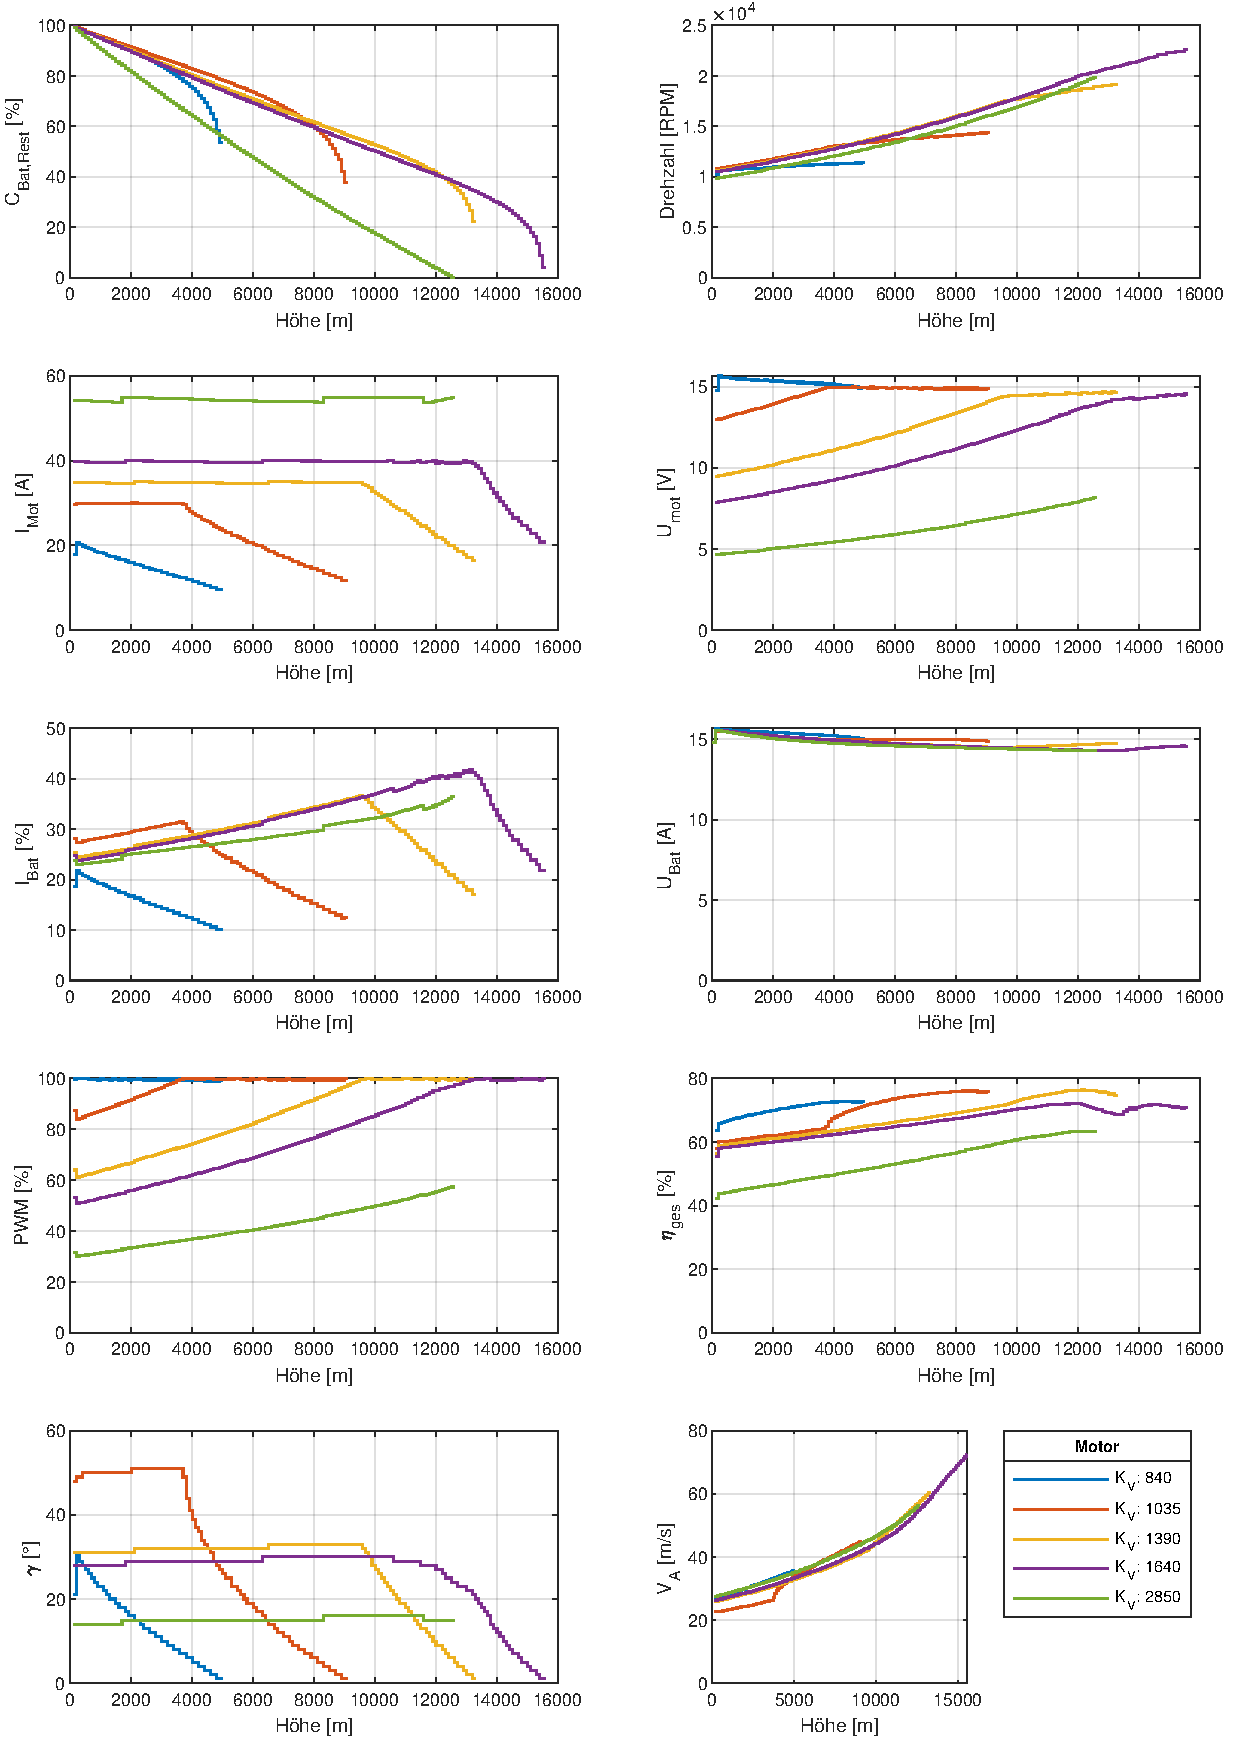
\includegraphics[scale=0.7]{Diagramme/Flaechenflzg_Mot_Prop.pdf}
	\caption{Einfluss der Motor-Propeller-Kombination auf die Flugleistungen der Flächenflugzeug-Referenzkonfiguration (Tab. \ref{tab:referenzkonfiguration})}
	\label{abb:flaechenflzg_mot_prop}
\end{figure}

Der \ensuremath{K_V}-Wert ist ein Kennwert für die Anzahl der Umdrehungen pro Minute pro Volt im Leerlauf. Ein hoher \ensuremath{K_V}-Wert bedeutet nun im Umkehrschluss, dass bei einer hohen Drehzahl die Spannung geringer ist als für einen Motor mit einem vergleichsweise niedrigem \ensuremath{K_V}-Wert. Die Drehzahl ist in diesem Fall für fast alle Motoren identisch bzw. die Unterschiede minimal. Gleichzeitig sinkt allerdings das Verhältnis von Drehmoment pro Ampere, das der \ensuremath{K_M}-Wert ausdrückt  \cite[S.35 und S.42-43]{Buchi.2013}. Es gilt die Beziehung
\begin{equation}
	K_M = 1/K_V\cdot 30/\pi \eqend{.}
\end{equation}
Ein Motor mit hohem \ensuremath{K_V}-Wert muss daher einen hohen Dauermotorstrom besitzen, um gute Flugleistungen zu erzielen (vgl. Abb. \ref{abb:flaechenflzg_mot_prop}). Durch diese Abhängigkeit wird auch die PWM beeinflusst. Der Motor mit einem \ensuremath{K_V} von \SI{840}{RPM/V} erreicht durch seine hohe Motorspannung deutlich schneller das Niveau der Batteriespannung und hat somit seinen Leistungsüberschuss aufgebraucht. Somit wird auch frühzeitiger das Absinken des Bahnneigungswinkels eingeleitet. Für Motoren mit einem niedrigeren \ensuremath{K_V}-Wert bedeutet dies auch gleichzeitig das Ende des Steigfluges. \\
Dieser Zusammenhang stellt sich für Motoren mit hohem \ensuremath{K_V}-Wert dar. Hier wird \SI{100}{\%} PWM erst bei deutlich größeren Höhen erreicht oder gar nicht, weshalb folglich der optimale Bahnneigungswinkel erst in größeren Höhen nicht mehr gehalten werden kann und danach sinkt. Bei \ensuremath{\gamma = \SI{0}{^\circ}} ist der Steigflug beendet. Hierbei steigt zudem der optimale Bahnneigungswinkel mit dem \ensuremath{K_V}-Wert. Da die Geschwindigkeit mit einem höheren Bahnneigungswinkel sinkt (vgl. Gleichung \eqref{eq:geschw_flaechenflugzeug}), sinkt auch die benötigte Leistung, die hauptsächlich für die Motoren mit geringem \ensuremath{K_V} begrenzend ist. Dabei nimmt die Restladung für kleinere \ensuremath{K_V}-Werte nicht so schnell ab wie dies für große \ensuremath{K_V}-Werte der Fall ist. Dies kann auf den höheren Gesamtwirkungsgrad und im Detail auf den höheren Motorreglerwirkungsgrad zurückgeführt werden. Durch die deutlich höhere Pulsweitenmodulation ist der Wirkungsgrad des Motorreglers entsprechend höher (vgl. Gleichung \eqref{eq:eta_pwm}). Außerdem sind die Verluste durch die Temperatur sowie Innenwiderstände oder den Leerlaufstrom für einen Motoren mit niedrigem \ensuremath{K_V}-Wert geringer. Der letzte starke Anstieg des Gesamtwirkungsgrades für \SI{840}{RPM/V} und \SI{1035}{RPM/V} liegt am Propellerwirkungsgrad. Durch den starken und schnellen Abfall des Bahnneigungswinkels steigt entsprechend die Fluggeschwindigkeit \ensuremath{V_A} signifikant an (vgl. Gleichung \eqref{eq:geschw_flaechenflugzeug}). Als Konsequenz auf den starken Anstieg der Fluggeschwindigkeit steigt auch der Propellerwirkungsgrad (vgl. Gleichung \eqref{eq:eta_prop}). \\
Zusammengefasst besitzen Motoren mit einem niedrigen \ensuremath{K_V}-Wert eine höhere Effizienz im Betrieb, die sich gegenüber Motoren mit einem höheren \ensuremath{K_V} vor allem in der Abnahme der Restladung zeigt. Allerdings ist die Leistung unzureichend für den in dieser Arbeit geforderten Aufstieg. Dies macht sich vor allem im Leistungsüberschuss bemerkbar. Ein zu hoher \ensuremath{K_V}-Wert des Motors bedeutet auf der anderen Seite jedoch wieder zu hohe Verluste und somit erneut eine nicht optimale Konfiguration des Flächenflugzeugs. Folglich liegt das Optimum in der Mitte der beiden Grenzen. Es ist also ein Motor mit einem hohen \ensuremath{K_V}-Wert zu wählen, der aber auch geringe interne Verluste und Verluste im Motorregler aufweist. Dies wird gut durch den hier verwendeten Motor mit 1390 \ensuremath{K_V} repräsentiert. \\
%Hier sei auch nochmal auf den Sprung im Verlauf der Leistungsgrößen für die Motoren mit 1390 und 1640 \ensuremath{K_V} hingewiesen. Da dieser bei beiden an der gleichen Stelle auftritt und die Drehzahlverläufe komplett identisch sind, kann dieser auf eine Inkonsistenz im Propellerkennfeld zurückgeführt werden.



\subsection{Anzahl der Motoren und Propeller}
\label{subsec:anz_mot_flaechenflzg}
Während die Leistung der Motoren mit gleichem Gewicht schon einen großen Einfluss auf den optimalen Steigwinkel hat, ändert sich dies entscheidend mit der Anzahl der Motoren (vgl. Abb. \ref{abb:flaechenflzg_n_prop}). Schon mit einer Steigerung der Motorenanzahl auf zwei verändert sich der optimale Steigwinkel zu \SI{90}{^\circ}. Die dazu zugehörige Steiggeschwindigkeit liegt hierbei beim Maximum der Iterationsweite von der Steiggeschwindigkeit (siehe Abschn. \ref{subsubsec:schub_flaechenflzg}).
Auch hier kann die Effektivität und Effizienz einer Propelleranzahlerhöhung wieder an dem Diagramm der Restladung festgemacht werden. Je mehr Propeller verwendet werden, desto schneller sinkt die Restladung auf \SI{0}{\%}. Dies ist für alle Konfigurationen bis auf die Referenzkonfiguration der Fall, die ihre Dienstgipfelhöhe erreicht. Mit Ausnahme für zwei Propeller sinkt mit steigender Anzahl der Propeller auch die maximal erreichbare Höhe. Der Schub ist für alle Konfigurationen ähnlich, jedoch wird dieser bei einer Propelleranzahl von größer eins auf die Propeller aufgeteilt. Damit sinkt die erforderliche Leistung pro Motor. Dies macht sich in einer Verringerung der Drehzahl bemerkbar, die wiederum in einer Verringerung des Motorstroms (siehe Gleichung \eqref{eq:motorstrom}) und der Motorspannung (vgl. Abb. \eqref{eq:motorspannung}) mündet. Dadurch erhöht sich in Summe der Batteriestrom (vgl. Gleichung \eqref{eq:batteriestrom}) und führt zu einem stärkeren Einbruch der Batteriespannung. Rückwirkend fällt durch die geringe Motorspannung auch die PWM äußerst niedrig aus (vgl. Gleichung \eqref{eq:pwm}), was den ESC-Wirkungsgrad \ensuremath{\eta_{PWM}} durch größere Verluste verschlechtert (vgl. Gleichung \eqref{eq:eta_pwm}). Der geringe Schub pro Propeller in Kombination mit der geringen Drehzahl vermindert den Propellerwirkungsgrad \ensuremath{\eta_{Prop}} (vgl. Gleichung \eqref{eq:eta_prop}), der zusammen mit dem ESC-Wirkungsgrad den Gesamtwirkungsgrad \ensuremath{\eta_{ges}} verringert.\\
Alle Flächenflugzeugkonfigurationen mit \ensuremath{n_{Prop}} größer eins haben gemeinsam, dass bis ca. \SI{9000}{m} Höhe ein Steigflug mit \SI{90}{^\circ} den effizientesten Steigflug bestimmt. 
Dies ist solange der optimale Betriebspunkt bis der Steigwinkel von \SI{55}{^\circ} ab ca. \SI{8500}{m} energieeffizienter ist. Ein vergleichbares Flugverhalten ist bei einer Erhöhung der Propelleranzahl auf 4 zu beobachten. Dies repräsentiert das Verhalten eines VTOL-Flugzeuges, dass mit \ensuremath{\gamma = 90^\circ} vertikal startet und ab \SI{9000}{m} Höhe in die Transition auf einen Bahnneigungswinkel von \SI{55}{^\circ} übergeht. 
Bemerkenswerter Weise sind die Kurven der Restladung von einem und zwei Propellern deckungsgleich, obwohl alle übrigen Leistungsparameter signifikant unterschiedliche Werte durch die veränderte Propelleranzahl und das durch den zusätzlichen Motor erhöhte Gewicht des Flächenflugzeugs aufzeigen. Dies bedeutet, dass der Vorteil der Schubhalbierung und der vertikale Steigflug gerade den Nachteil des zusätzlichen Motorgewichts kompensieren. Der zweite Übergang in den vertikalen Steigflug ab \SI{16500}{m} stellt einen ineffizienten Flugzustand dar, was vor allem durch den Verlauf der Restladung und des Gesamtwirkungsgrades reflektiert wird. Ein Grund für den Übergang liegt in dem verringerten Widerstand im vertikalen Steigflug. Dieser entspricht nur noch dem Nullwiderstand (vgl. Gleichung \eqref{eq:widerstand_vertikalflug}). Für einen Steigflug mit einem Bahnneigungswinkel \ensuremath{\gamma} von weniger als \SI{90}{^\circ} wächst der Widerstand quadratisch mit der progressiv ansteigenden Geschwindigkeit (vgl. Gleichung \eqref{eq:geschwindigkeit_skalierung}).\\
Insgesamt verringert eine Erhöhung der Motor- und Propelleranzahl um zwei den TOC um ca. \SI{7500}{m}. Die optimale Propelleranzahl ist in diesem Fall zwei, weil mit dieser Anzahl die Dienstgipfelhöhe in weitere Höhen verschoben wird.
(Der kurze Sprung bei \ensuremath{n_{Prop} = 6} wird in der Untersuchung vernachlässigt).

\begin{figure}[H]
\centering
	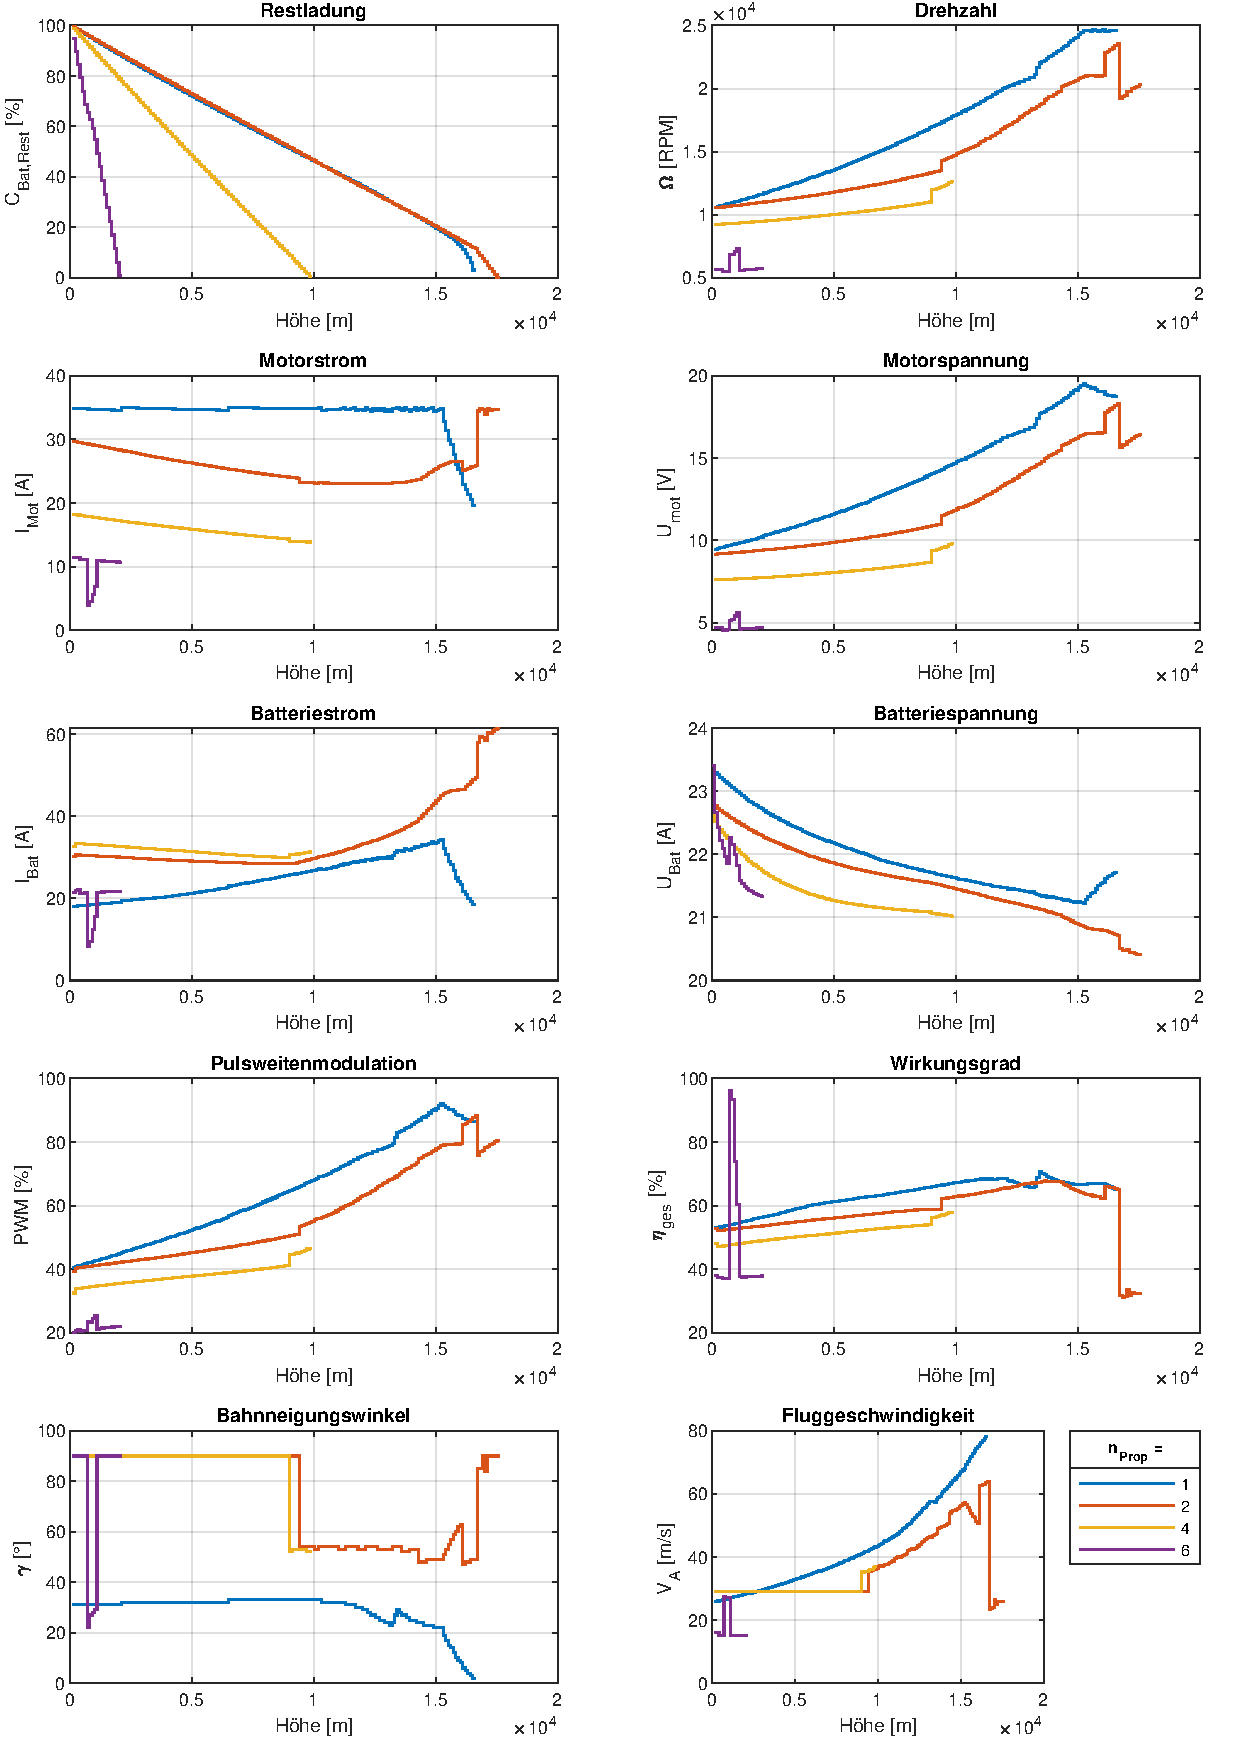
\includegraphics[scale=0.7]{Diagramme/Flaechenflzg_n_prop.pdf}
	\caption{Einfluss der Propelleranzahl auf die Flugleistungen der Flächenflugzeug-Referenzkonfiguration (Tab. \ref{tab:referenzkonfiguration})}
	\label{abb:flaechenflzg_n_prop}
\end{figure}


\subsection{Gleitzahl}
\label{subsec:gleitzahl}
Der Einfluss der Gleitzahl äußert sich hauptsächlich in der Effizienz des Flächenflugzeugkonfiguration, die wiederum durch die Abnahme der Restladung ausgedrückt wird (vgl. Abb. \ref{abb:gleitzahl})
Alle Verläufe erreichen die Dienstgipfelhöhe, die durch die maximale Propellerdrehzahl \ensuremath{\Omega_{Prop}} limitiert wird. Ohne diese limitierende Höhe könnte das Flächenflugzeug bei linearer Extrapolation der Restladungskurve sogar mit einer Gleitzahl von 50 eine Höhe von ca. \SI{25000}{m} erreichen. 
Mit einer Verringerung der Gleitzahl geht auch eine Verringerung der maximalen Höhe mit einher und umgekehrt. Eine entsprechend hohe Gleitzahl bedeutet gleichzeitig auch eine hohe aerodynamische Güte (vgl. \cite[S.34]{Scheiderer.2008}). Dazu sinkt der Widerstand im Vergleich zum Auftrieb, sodass für ein Flächenflugzeug mit einer höheren Gleitzahl (vgl. Gleichung \eqref{eq:gleitzahl}) für den gleichen Auftrieb weniger Leistung zur Kompensation des Widerstandes aufgebracht werden muss. Als Konsequenz dessen steht mehr Leistung für das Steigen zur Verfügung. Mit der Gleitzahl steigt ebenso der optimale Bahnneigungswinkel. Als Grund dafür kann wieder die verringerte Widerstandsleistung angeführt werden. Zusätzlich sinkt die Zeit zum Überwinden einer Höhendifferenz mit einem steileren Winkel. Einen Änderung der Gleitzahl hat nur einen Einfluss auf die Restladung, die Batteriespannung und den Bahnneigungswinkel. Eine geringe Gleitzahl bedeutet einen stärkeren Einbruch der Batteriespannung, da wiederum für den gleichen Auftrieb mehr Widerstand kompensiert werden muss. \\
Auffällig ist noch die Flugleistungsverbesserung mit der Gleitzahl. Diese macht sich im Verlauf der Restladung deutlich bemerkbar. Eine Verbesserung der Gleitleistung von \ensuremath{E = 4} auf \ensuremath{E = 6} bedeutet auf einer Höhe von \SI{15000}{m} bereits \SI{10}{\%} mehr Restladung und einen \SI{7}{^\circ} höheren Bahnneigungswinkel. Eine erneute Erhöhung der Gleitzahl auf 10 steigert die Restladung auf dieser Höhe über dem  Meereslevel nur noch um \SI{5}{\%} und eine Erhöhung des Bahnneigungswinkel \SI{5}{^\circ}. Dieser Trend der abnehmenden Flugleistungsoptimierung bei einer gleichzeitigen Verdoppelung der Gleitleistung setzt sich fort (siehe \ref{abb:gleitzahl}).
Das einfache Flächenflugzeugmodell berücksichtigt nicht, dass eine Gleitzahlerhöhung auch mit einer deutlichen Erhöhung der Strukturmasse einhergeht, weil die Flugzeugzelle, die Flügelform, das Flügelprofil usw. an die neuen Bedingungen angepasst und verstärkt werden müssen. Dieser Zusammenhang wird beim Vergleich der Gleitleistung eines Segelflugzeugs mit dessen Spannweite deutlich. \\
Dementsprechend ist eine Erhöhung des Penalty-Faktors zwingend erforderlich. Unter Berücksichtigung dieser Zusammenhänge gilt es einerseits die Gleitleistung des Flächenflugzeugs für eine Verbesserung der Flugleistungen zu steigern, dies auf der anderen Seite mit der zusätzlichen Masse der Flugzeugstruktur und dem tatsächlichen Gewinn an Flugleistungen abzuwägen. Es ist zu mutmaßen, dass eine Gleitzahl zwischen 6 und 10 die besten Ergebnisse erzielt.

\begin{figure}[H]
\centering
	
\includegraphics[scale=0.7]{Diagramme/Flaechenflzg_E.pdf}
	\caption{Einfluss der Gleitzahl auf die Flugleistungen der Flächenflugzeug-Referenzkonfiguration (Tab. \ref{tab:referenzkonfiguration})}
	\label{abb:gleitzahl}
\end{figure}


\subsection{Auslegungsgeschwindigkeit}
\label{subsec:vstern}
Die Auslegungsgeschwindigkeit ruft ähnlich zu der Motor-Propeller-Kombination (vgl. Abb. \ref{abb:flaechenflzg_mot_prop}) oder der Propelleranzahl (vgl. Abb. \ref{abb:flaechenflzg_n_prop}) Einflüsse auf das Leistungsverhalten des Flächenflugzeugs hervor. Da für den Steigflug ein Flug mit konstantem Auftriebsbeiwert vorausgesetzt wird, erhöht sich aufgrund dessen die Fluggeschwindigkeit mit der Höhe und größerem Bahnneigungswinkel (vgl. Gleichung \eqref{eq:geschw_flaechenflugzeug}).
Ist die Auslegungsgeschwindigkeit gering, so wächst sie absolut gesehen mit der Höhe nicht so stark wie bei hohen Auslegungsgeschwindigkeiten (vgl. Verlauf der Fluggeschwindigkeit über der Höhe in Abb. \ref{abb:vstern}). 
Bis zu einem \ensuremath{V^\star} von \SI{75}{km/h} ist die Batterierestladung der limitierende Faktor für die Flughöhe. Ab einer Auslegungsgeschwindigkeit von \SI{100}{km/h}, die auch diejenige der Referenzkonfiguration ist, wird wieder die Dienstgipfelhöhe durch \ensuremath{Ma_{tip} = 1} an der Propellerblattspitze erreicht. Bis zu einer Höhe von \SI{13000}{m} sind auch die Verläufe der Restladung von \ensuremath{V^\star} mit \SI{100}{km/h} und \SI{125}{km/h} identisch. Für alle Auslegungsgeschwindigkeiten ist das Flugverhalten gleich dem aus Abschn. \ref{sec:multicopter_vs_flaechenflugzeug}. Es wird wieder solange mit maximalen Motorstrom geflogen, bis entweder die Restkapazität \SI{0}{\%} oder die Dienstgipfelhöhe durch einen anderen limitierenden Leistungsparameter, in diesem Fall wieder die Propellerdrehzahl, erreicht ist. Durch die höhere Auslegungsgeschwindigkeit und demzufolge auch die höhere Fluggeschwindigkeit (vgl. Gleichung \eqref{eq:geschw_flaechenflugzeug}) kommt es zu einer höheren Propelleranströmgeschwindigkeit. Um trotzdem den gleichen Schub zu erzeugen ist eine höhere Drehzahl notwendig. Mit dem schneller drehenden Propeller steigt auch die Motorspannung (vgl. Gleichung \eqref{eq:motorspannung}), der Batteriestrom und über die Motorspannung auch die PWM. Die gesteigerte Propelleranströmgeschwindigkeit verbessert den Propellerwirkungsgrad und als Konsequenz daraus den Gesamtwirkungsgrad. Daher ist der Gesamtwirkungsgrad für größere Auslegungsgeschwindigkeiten besser. Dies kann auch auf den verbesserten Motorreglerwirkungsgrad bei einer höheren PWM zurückgeführt werden (vgl. Gleichung \eqref{eq:eta_pwm}). Es kann schließlich noch festgehalten werden, dass mit steigender Auslegungsgeschwindigkeit der Bahnneigungswinkel \ensuremath{\gamma} abnimmt, da die Zeit zum Überwinden eines Höhenschritts bei einer höheren Geschwindigkeit und geringerem Bahnneigungswinkel sich kaum ändert. \\
Aufgrund dieser Tatsachen ist das Flächenflugzeug auf einigermaßen hohe Fluggeschwindigkeiten von rund \SI{100}{km/h} auszulegen, um zum einen den Leistungsüberschuss der Motoren ausreichend hoch zu halten und zum anderen die Zeit zum Aufstieg nicht zu vergrößern. Weiterhin wird die Auslegungsgeschwindigkeit durch die Wahl des Propellers beeinflusst. Bei gleichem Durchmesser steigt die optimale Auslegungsgeschwindigkeit mit der Propellersteigung.


\begin{figure}[H]
\centering
	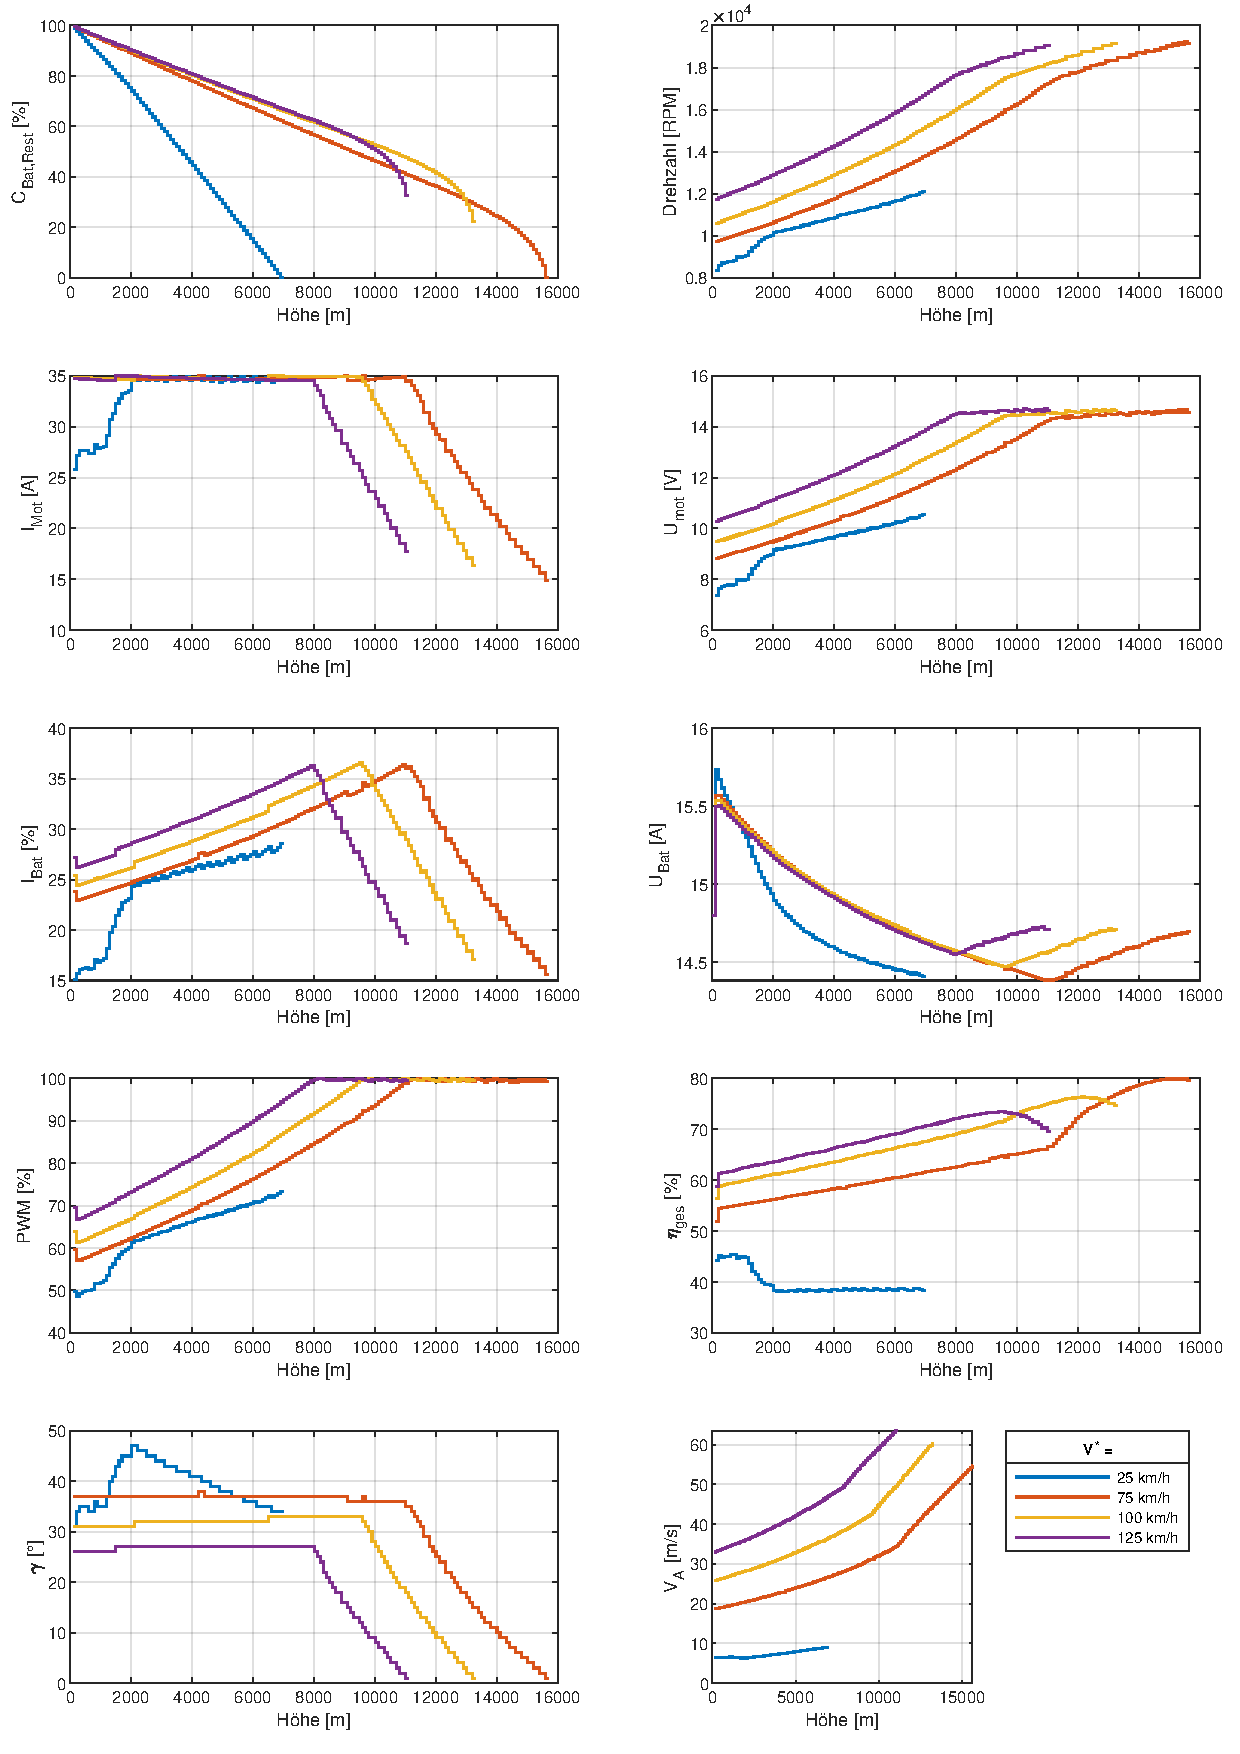
\includegraphics[scale=0.7]{Diagramme/Flaechenflzg_Vstern.pdf}
	\caption{Einfluss der Auslegungsgeschwindigkeit auf die Flugleistungen der Flächenflugzeug-Referenzkonfiguration (Tab. \ref{tab:referenzkonfiguration})}
	\label{abb:vstern}
\end{figure}



\subsection{Penalty-Faktor}
\label{subsec:f_p}
Beim Vergleich von einem Flächenflugzeug mit einem Multicopter muss bei gleichem Gesamtgewicht die unterschiedliche Verteilung der Gewichtskomponenten berücksichtigt werden. Für ein Flugzeug ist das Strukturgewicht von Flügeln und Rumpf sowie den Steuerungselementen bedeutend größer als das von einem Multicopter. Ein Penalty-Faktor von 1 entspricht daher wie oben beschrieben einer optimistischen Einschätzung, wenn beide Strukturgewichte bei einem gleichen Gesamtgewicht äquivalent sind. Um realistischere Ergebnisse für ein Flächenflugzeug zu erreichen, wird der Penalty-Faktor schrittweise erhöht. Dabei verringert sich auch die maximal erreichbare Höhe.
Der Einfluss des Penalty-Faktors konzentriert sich auf die Restladung und die Batteriespannung (vgl. Abb. \ref{abb:fp}). Dies hängt damit zusammen, dass ein Penalty-Faktor größer als 1 die zur Verfügung stehende Batteriemasse (vgl. Gleichung \eqref{eq:penalty}) und folglich die Batteriekapazität (vgl. Gleichung \eqref{eq:batteriekapazitaet}) reduziert. Die Referenzkonfiguration mit \ensuremath{f_P = 1} ist die einzige Konfiguration, die bis zur Dienstgipfelhöhe aufsteigt. Bei allen anderen nimmt die Restladung vorher \SI{0}{\%} an. Die Gesamtmasse ist unabhängig vom Penalty-Faktor identisch für jede Konfiguration, weshalb auch der Schub der gleiche ist und alle übrigen Verläufe der Leistungsparameter identisch sind. 
Aufgrund der Tatsache, dass die Batteriekapazität mit der Batteriemasse abnimmt, der Batteriestrom jedoch gleich bleibt, wird die Entladerate bezogen auf die Kapazität größer (vgl. Gleichung \eqref{eq:c_rate}). Dies ist der Grund für den zunehmenden Spannungsabfall der Batterie bei einem höheren Penalty-Faktor.\\
Insbesondere in Bezug auf Abschn. \ref{subsec:gleitzahl} ist der Penalty-Faktor von Bedeutung. Einer Anpassung der Flächenflugzeugzelle in Richtung einer Flugleistungsverbesserung sind Grenzen gesetzt. 


\begin{figure}[H]
\centering
	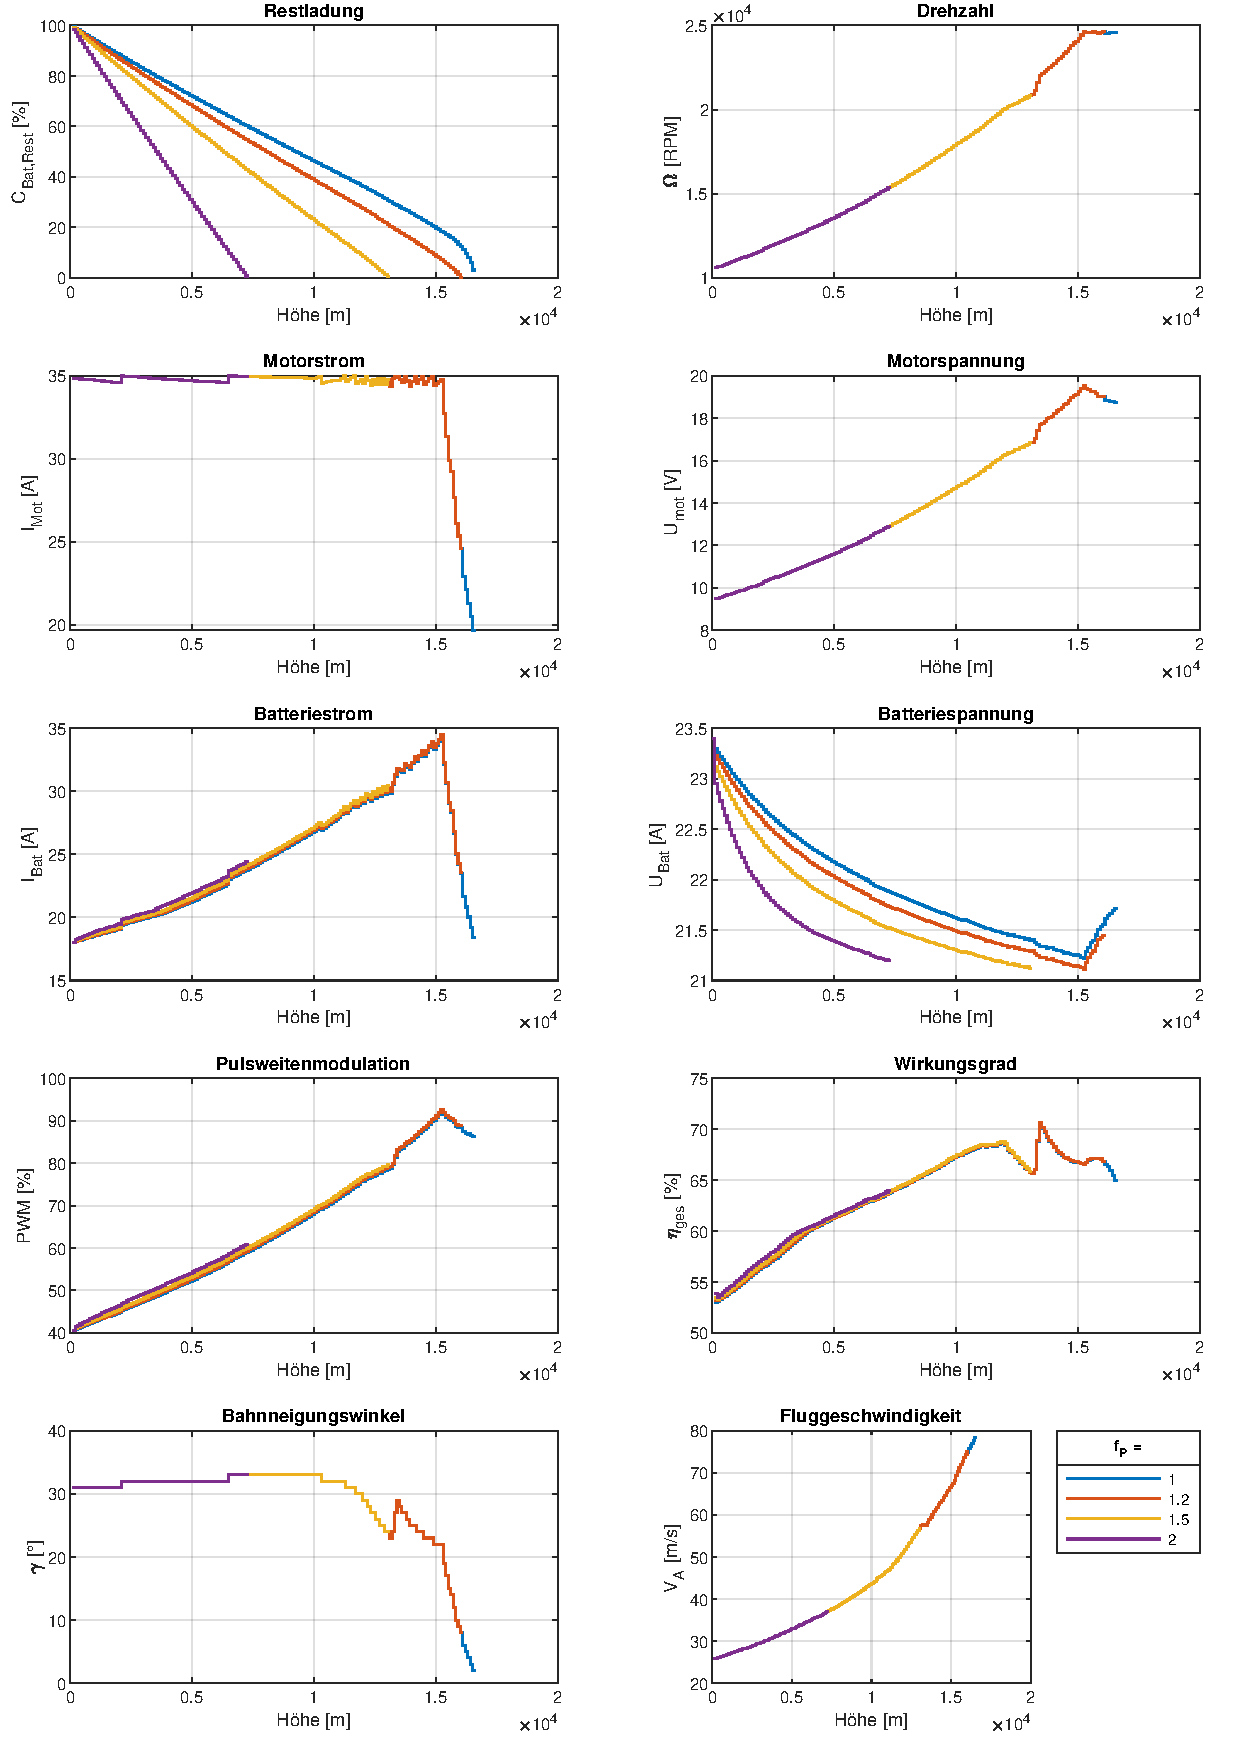
\includegraphics[scale=0.7]{Diagramme/Flaechenflzg_fp.pdf}
	\caption{Einfluss des Penalty-Faktors auf die Flugleistungen der Flächenflugzeug-Referenzkonfiguration (Tab. \ref{tab:referenzkonfiguration})}
	\label{abb:fp}
\end{figure}

\subsection{Zusammenfassung}
Aus den Ergebnissen wird ersichtlich, dass es viele Einflussfaktoren auf die Flugleistungen eines Flächenflugzeug für einen Steigflug auf \SI{10}{km} oder sogar \SI{15}{km} Höhe gibt. Zuerst sollte ein Motor mit einem vergleichsweise hohem \ensuremath{K_V}-Wert in seiner Gewichtsklasse gewählt werden, wobei der Propeller an den Motor anzupassen ist (vgl. Abschn. \ref{subsec:mot_prop_kombi}). Zur Vermeidung transsonischer Effekte sollte der Propellerdurchmesser entsprechend groß gewählt werden, was auch für die Steigung gilt. Die optimale Anzahl der Propeller liegt bei einem oder zwei. Je nach der Propelleranzahl variiert der effizienteste Bahnneigungswinkel, sodass bei einer Propelleranzahl von mindestens zwei das Flächenflugzeug als VTOL-Fluggerät am effizientesten fliegt (vgl. Abschn. \ref{subsec:anz_mot_flaechenflzg}). Weiterhin ist die Gleitleistung so groß wie möglich zu halten (vgl. Abschn. \ref{subsec:gleitzahl}). Hierbei sind einer solchen Erhöhung durch den Penalty-Faktor Grenzen gesetzt (vgl. Gleichung \ref{subsec:f_p}). Die Auslegungsgeschwindigkeit ist an den Propeller anzupassen und so hoch wie möglich zu wählen, um einen Kompromiss aus verbesserter Steiggeschwindigkeit und verringerter Schuberzeugung durch den Propeller zu finden (vgl. Abschn. \ref{subsec:vstern}). In diesem Rahmen ist die Referenzkonstruktion bereits sehr gut ausgelegt.\\


\section{Ergebnisse des Vergleichs}
\label{sec:ergebnisse_vergleich} 
Im direkten Vergleich weist das Flächenflugzeug eine größere maximale Flughöhe (vgl. z.B. Abb. \ref{abb:referenzkonfiguration}) auf als der Quadrocopter aus \cite{Anderson.2018}. Besonders mit hohen Gleitzahlen (vgl. Abschn. \ref{subsec:gleitzahl}), mehreren Motoren (vgl. Abschn. \ref{subsec:anz_mot_flaechenflzg}) und einer guten Kombination aus Motor und Propeller (vgl. Abschn. \ref{subsec:mot_prop_kombi}) wird dieser Vorteil ersichtlich. Jedoch vernachlässigt das einfache Modell des Flächenflugzeugs zusätzliche Widerstände. Die Vorteile eines Flächenflugzeuges zeigen sich auch nur bei einem Penalty-Faktor nahe eins. Dies muss als unrealistisch angesehen werden. Besonders im Bezug auf eine hohe Gleitzahl geht diese Anforderung mit einer hohen Flügelstreckung und damit mit einem hohen Strukturgewicht einher. Somit ist es zwingend notwendig den Penalty-Faktor zu erhöhen. Werden diese Einschränkungen berücksichtigt, schwindet der zusätzliche Höhengewinn eines Flächenflugzeugs gegen Null. Weiterhin erweist sich das Flächenflugzeug als bereits in den möglichen Maßen im Rahmen dieses Modells als optimiert. Die Steiggeschwindigkeit ist in Bezug auf den Auslegungszustand und einem Flug bei Auslegungsgleitzahl optimal. Außerdem wird der Steigwinkel für jeden Höhenabschnitt optimiert (vgl. Abschn. \ref{subsubsec:schub_flaechenflzg}) und eine gute Kombination von Motor und Propeller ist bereits gegeben (vgl. Abschn. \ref{sec:flaechenflugzeug_referenzkonfig}). Schlussendlich ist damit der Spielraum für weitere Verbesserungen eingeschränkt. Ohne die Limitierung durch den Propeller könnte ein  ideales Flächenflugzeug Höhen von mehr als \SI{18000}{m} erreichen. \\
Hingegen zeigt der Quadrocopter in dieser Hinsicht noch Potential. %Ein zu untersuchender Punkt ist noch die Abkehr von einer konstanten Steiggeschwindigkeit hin zu einer kontinuierlichen Optimierung mit der Höhe. %Das Flächenflugzeugmodell aus Abschn. \ref{subsubsec:schub_flaechenflzg} vernachlässigt hier die Abhängigkeit des Flugzeugentwurfs von der Masse. Jede Designänderung verändert die Konstruktion des Flächenflugzeugs z.B. die Struktur und dessen Stärke, das Fahrwerk, den Motor und so weiter. Dieser Zusammenhang findet in dem Flächenflugzeugmodell nur durch die Wahl des Penalty-Faktors Berücksichtigung. \\
Wird für das Flugzeug außerdem eine Konstellation von mehr als einem Motor gewählt, neigt das Flugzeug dazu in einem \SI{90}{^\circ} Winkel zu steigen (vgl. Abschn. \ref{subsec:anz_mot_flaechenflzg}). Damit zeigt sich die optimale Flugweise in einem vertikalen Steigflug. Hierbei werden nichtsdestotrotz wieder viele Vereinfachungen getroffen und Verluste nicht berücksichtigt. 
In der Berechnung der Flächenflugzeugaerodynamik bleibt der Einfluss von Seitenwinden unberücksichtigt, da Seitenwinde nur die Strecke über Grund beeinflussen nicht aber die Flugeigenschaften im Steigflug (siehe Kap. \ref{subsubsec:schub_flaechenflzg}). Unter Berücksichtigung an das angedachte Operationsziel, einer Atmosphärenmessung, sind die Flugkorridore, die von der Deutschen Flugsicherung (DFS) zur Verfügung gestellt werden, begrenzt. Daher ist eine Abdrift bei sehr hohen Seitenwinden für die Mission negativ und muss vom Fluggerät ausgeglichen werden. Dies verbraucht zusätzlich Energie zum Ausgleichen und reduziert nochmals die erreichbare Höhe. Beim Quadrocopter geschieht das bereits durch den Ausgleich der Seitenwinde mit einer Anpassung vom Winkel \ensuremath{\alpha_{M}}, also einer Neigung der Rotorebene. Ein weiteres Argument, was gegen den Einsatz von einem Flächenflugzeug spricht ist, dass eine Start und Landevorrichtung von Nöten ist. Das erfordert Platz für eine Start- und Landebahn. Aufgrund seiner Senkrechtstarterfähigkeit benötigt der Multicopter wenig Platz zum Starten und Landen. 
Entsprechend dieser Argumentation wird in dieser Arbeit entschieden, dass ein Multicopter gegenüber einem Flächenflugzeug für einen Steigflug in die untere Stratosphäre als vorteilhafter anzusehen ist.
    \chapter{Optimierung weiterer Parameter}
\label{chap:optimierung_parameter}
Grundlegend kann die Parameteruntersuchung wie eine Art Entscheidungsbaum aufgefasst werden. Dabei führt jede Entscheidung im Baum zu einer neuen Untersuchung und zu neuen Erkenntnissen. Im Verlaufe dieser Untersuchung werden somit Konzepte, Flugzustände, Komponenten und Konfigurationen ausgewählt und intensiver betrachtet. Zuerst wird eine Multicopter-Referenzkonfiguration in Kap. \ref{sec:multicopter_referenzkonfig} definiert. Danach folgt die Untersuchung einzelner Parameter auf die Flugleistungen der Referenzkonfiguration (vgl. Kap. \ref{sec:einfluss_multicopter_referenzkonfiguration}). Schließlich wird noch eine optimale Lösung vorgeschlagen und der Einfluss der AEROMET\_UAV-Randbedingungen auf diese genauer betrachtet (vgl. Kap. \ref{sec:otimale_lsg}).\\
In der folgenden Parameteruntersuchung sei nochmal auf den Aufbau der Leistungsberechnung verwiesen, der dem eines realen Systems in umgekehrter Weise gegenübersteht (Kap. \ref{sec:flugleistungsberechnung}).


\section{Multicopter-Referenzkonfiguration}
\label{sec:multicopter_referenzkonfig}
Im Folgenden soll analog zum Flächenflugzeug eine Referenzkonfiguration für einen Multicopter in Tab. \ref{tab:referenzkonfiguration_mulitcopter} festgelegt werden. Die gewählte Konfiguration ergibt sich aus vorangegangenen Untersuchungen sowie Erfahrungswerten. 

\begin{center}
	\captionof{table}{wichtige Parameter der Multicopter-Referenzkonfiguration}
	\begin{tabular}{l l l} \hline
		Parameter & Variablenname & verwendete Größe \\ \hline
		Gesamtmasse \ensuremath{m} & \texttt{m} & \SI{3,078}{kg} \\
		Leermasse des Multicopters \ensuremath{m_{copter}}& \texttt{m\_copter} & \SI{1.028}{kg} \\ 
		Batteriemasse \ensuremath{m_{Bat}} & \texttt{m\_Bat} & \SI{1,626}{kg} \\
		Motormasse \ensuremath{m_{Mot}}& \texttt{m\_Mot} & \SI{106}{g} \\
		Geschwindigkeitskonstante \ensuremath{K_V} & \texttt{K\_V} & \SI{1390}{RPM/V} \\
		maximaler Dauerstrom \ensuremath{I_{max}} & \texttt{I\_max} & \SI{35}{A} \\
		Propeller & \texttt{prop\_name} & 11x3 \\
		Anzahl Propeller \ensuremath{n_{Prop}} & \texttt{n\_prop} & \SI{4}{} \\ 
		Anzahl der Batteriezellen \ensuremath{N_{Bat,cell}} & \texttt{N\_bat\_cell} & 6 \\	 
		Obere Stirnfläche \ensuremath{F_{copter,oben}} & \texttt{F\-copter\_oben} & \SI{0,0209}{m^2} \\
		Oberer Widerstandsbeiwert \ensuremath{c_{W,copter,oben}} & \texttt{c\_W\_copter\_oben} & 1 \\ \hline
	\end{tabular}	
	\label{tab:referenzkonfiguration_mulitcopter}
\end{center}

Die Umgebungsparameter sind die für eine Standardatmosphäre auf Meereshöhe (entspr. QNH). Dazu wurde der Seitenwind nicht wie im AEROMET\_UAV Projekt auf \SI{100}{km/h} sondern auf konstante \SI{10}{m/s} festgesetzt. Der Grund hierfür ist, dass der Leistungsüberschuss in einem mäßig schnellen Vorwärtsflug am größten ist \cite[S.328-S.329]{Wall.2015}. Dieser Zusammenhang wird mit der Windgeschwindigkeit modelliert. Außerdem kann der Einfluss einzelner Parameter besser und genauer untersucht werden. Die AEROMET\_UAV Randbedingungen werden später in Abschn. \ref{subsec:aeromot_rb} berücksichtigt.

\section{Einflussfaktoren auf die Multicopter-Referenzkonfiguration}
\label{sec:einfluss_multicopter_referenzkonfiguration}
Für einen Multicopter gibt es viele Einflussfaktoren, die im Folgenden genauer betrachtet werden sollen.

\subsection{Einfluss des Luftwiderstands}
\label{subsec:widerstandseinfluss}
Der Widerstandsbeiwert hat einen Einfluss auf die Flugleistungen eines Multicopters, der als gering eingeschätzt werden kann (vgl. Abb. \ref{abb:c_W_einfluss}). Unabhängig von dem Widerstandsbeiwert \ensuremath{c_W} endet für alle Konfigurationen der Steigflug bei der Dienstgipfelhöhe. Auch hier stellt die Prepellerdrehzahl den die Höhe limitierenden Parameter dar, die ab \SI{20100}{RPM} eine Blattspitzengeschwindigkeit \ensuremath{Ma_{tip}} von \ensuremath{Ma = 1} erreicht. Das Erreichen der Dienstgipfelhöhe wirkt sich jedoch kaum auf die Restladung aus.\\
Bis zu einer Höhe von \SI{15000}{m} erfolgt der Steigflug bei maximalen Motorstrom \ensuremath{I_{max}}. Mit dem Schub und der abnehmenden Dichte steigt die Drehzahl, die in einer Erhöhung der Motorspannung mündet. Durch die Belastung fällt die Batteriespannung ab, sodass diese in Kombination mit der Motorspannung in einer PWM Erhöhung resultiert. Nach einem anfänglichen Anstieg auf ca. \SI{52,5}{\%} fällt der Gesamtwirkungsgrad \ensuremath{\eta_{ges}} auf \SI{41,5}{\%} ab. 
Am deutlichsten kann der Einfluss des Widerstandsbeiwertes an dem Verlauf der Restladung und der Bahngeschwindigkeit ausgemacht werden. 
Bei einem großen maximalen Motorstrom gilt, dass die Begrenzung der Geschwindigkeit durch den Widerstandsbeiwert erfolgt. Eine sehr hohe Geschwindigkeit verringert zum einen die Flugzeit für einen Höhenschritt, erhöht auf der anderen Seite jedoch den Widerstand und damit zusätzlich die benötigte Leistung (vgl. Gleichung \eqref{eq:widerstand}). Je geringer der \ensuremath{c_W}-Wert gewählt wird, desto höher ist die optimale Bahngeschwindigkeit. Erhöht sich im Umkehrschluss der Luftwiderstand so sinkt die Bahngeschwindigkeit, da der Widerstand mit der Geschwindigkeit quadratisch (vgl. Gleichung \eqref{eq:widerstand}) ansteigt. Zudem erhöht ein geringer Widerstandsbeiwert die vorhandene Restkapazität. Anhand der Restkapazitätsabnahme kann ein beinahe lineare Abhängigkeit zwischen einer \ensuremath{c_W}-Erhöhung und einer Abnahme der Restladung festgestellt werden. Im Schnitt sinkt mit einer Anhebung des \ensuremath{c_W}-Wertes um 0,5 die Restladung auf \SI{15000}{m} um \SI{4}{\%}. Im Vergleich zum Einfluss der Gleitzahl auf die Flugleistungen eines Flächenflugzeuges ist der Verlauf hier ähnlich (vgl. Abb. \ref{subsec:gleitzahl}). 
Im Sinne einer großen maximalen Höhe ist daher eine aerodynamisch günstige Verkleidung des Multicopters anzustreben.
  
\begin{figure}[H]
\centering
	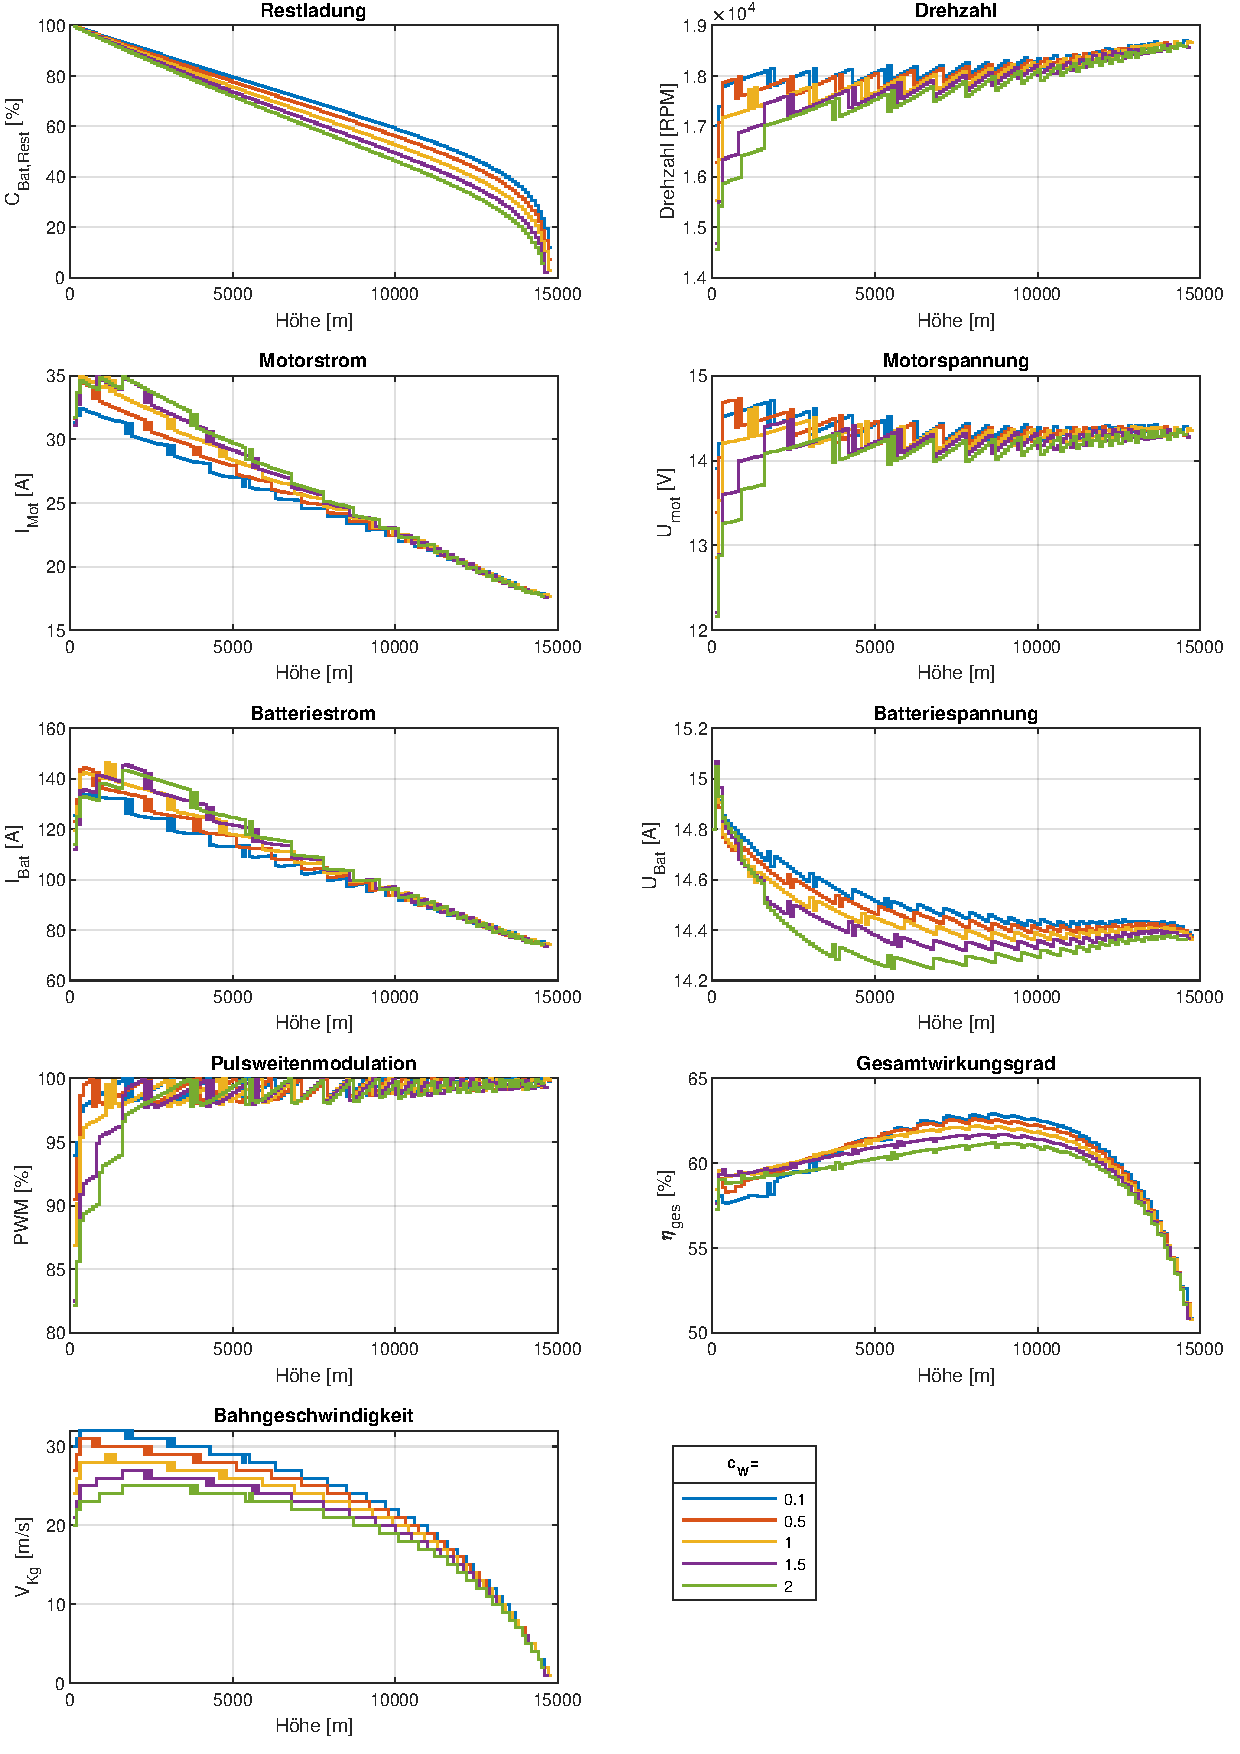
\includegraphics[scale=0.7]{Diagramme/Untersuchung_c_W.pdf}
	\caption{Einfluss des Widerstandsbeiwertes auf die Flugleistungen der Multicopter-Referenzkonfiguration (Tab. \ref{tab:referenzkonfiguration_mulitcopter})}
	\label{abb:c_W_einfluss}
\end{figure}


\subsection{Einfluss der Batteriespannung}
\label{subsec:einfluss_n_bat}
Wie in Kap. \ref{subsec:mot_prop_kombi} gezeigt, ist ein weiterer begrenzender Parameter die max. Motorleistung bzw. die PWM. Die Motorspannung an sich kann nicht beeinflusst werden. Jedoch lässt sich Einfluss auf die Höhe der Motorspannung durch eine Erhöhung der in Reihe geschalteten Batteriezellen nehmen. Mit jeder zusätzlichen Zelle erhöht sich die nominelle Batteriespannung um \SI{3,7}{V} (vgl. Abb. \ref{abb:N_Bat_einfluss}). Damit stellt die PWM nicht mehr die Grenze für die Bahngeschwindigkeit dar. Der effizienteste Flugzustand ist nun der beim maximalen, dauerhaften Motorstrom. Jedoch führt bei gleicher Energiemenge und somit gleicher Masse 
\begin{equation}
	E_{Bat} = C_{Bat}\cdot U_{Bat}
\end{equation}
eine Erhöhung der Spannung in dem Produkt aus Spannung und Kapazität (\ensuremath{C_{Bat} = I_{Bat}\cdot t_{Flug}}) unweigerlich zu einer Verringerung der Kapazität.  \\
Alle Batteriekonfigurationen steigen bis zu ihrer Dienstgipfelhöhe auf. 
Für die Batterie mit nur zwei Zellen ist diese durch die PWM bei \SI{100}{\%} bereits kurz nach Beginn des Steigfluges erreicht. Der Grund dafür ist der aufgebrauchte Leistungsüberschuss. Die Motorspannung ist durch die Batteriespannung (und die PWM) begrenzt, weshalb die Propellerdrehzahl auch begrenzt ist. Folglich ist der Schub beschränkt, was zu einer Abnahme der Bahngeschwindigkeit auf \SI{0}{m/s} führt. \\
Deutlich bessere Ergebnisse liefert eine Verdoppelung der Zellenanzahl auf vier. Diese Konfiguration erreicht auch die Dienstgipfelhöhe, jedoch ist das Niveau der nominellen Batteriespannung im Gegensatz zu der zweizelligen Batterie doppelt so hoch. Dies bedeutet, dass zu Beginn des Fluges der Motor wieder am effizientesten mit maximalem Strom \ensuremath{I_{max}} betrieben werden kann. Im Laufe des Fluges steigt die Drehzahl des Propellers und somit die auch die Motorspannung (vgl. Gleichung \eqref{eq:motorspannung}). Dieser Betriebszustand ist wieder solange möglich bis kein Leistungsüberschuss mehr vorhanden ist und die PWM \SI{100}{\%} erreicht. Es kommt zu einer Limitierung der Drehzahl durch die Motorspannung und letztendlich zum immer schneller werdenden Absinken der Bahngeschwindigkeit. \\
Die Leistungsparameter für die Batterien mit mehr als vier Zellen in Reihe sind in Bezug auf die Restladung die Propellerdrehzahl, den Motorstrom und die -spannung sowie die Bahngeschwindigkeit beinahe identisch. Lediglich in den Batteriekenngrößen und damit auch in der PWM treten Unterschiede auf, weil mit der Zellenanzahl die nominelle Batteriespannung steigt und damit die PWM sinkt (vgl. Gleichung \eqref{eq:pwm}). Der Batteriestrom nimmt ebenfalls durch die sinkende PWM ab. Die Dienstgipfelhöhe ist analog zu Abschn. \ref{subsec:widerstandseinfluss} durch die maximale Propellerdrehzahl und diese wiederum durch die Blattspitzengeschwindigkeit begrenzt. \\
Ein Optimum für die günstigste Anzahl an Batteriezellen liegt bei \ensuremath{N_{Bat,cell} = 4} vor, da diese Konfiguration in jedem Höhenschritt die größte Restladung aufweist (vgl. Abb. \ref{abb:N_Bat_einfluss}). Dies ist jedoch einzuschränken. Diese Konstellation erreicht die geringste Abnahme der Restkapazität mit der Höhe, jedoch schränkt die im Vergleich zu Batterien mit mehr Zellen geringere, nominelle Batteriespannung die Motorleistung ein, was zu einem frühzeitigen Beenden des Steigflugs durch Erreichen der Dienstgipfelhöhe führt. Dieser Flaschenhals ist bei mindestens einer Zelle mehr nicht mehr gegeben. In diesem Sinne ist eine fünfzellige Batterie für die Multicopter-Referenzkonfiguration zu bevorzugen. Jedoch weist die vierzellige Batterie den größten Gesamtwirkungsgrad auf. Dieser fällt ebenfalls mit der nominellen Batteriespannung. Insbesondere für die Batterien mit mehr als vier Zellen sind der Propeller- und Motorwirkungsgrad identisch, da die Leistungsgrößen, die auf diese Wirkungsgrade einen Einfluss haben, ebenfalls identisch sind. \\
Der Grund für die unterschiedlichen Gesamtwirkungsgrade liegt im Wirkungsgrad des Motorreglers. Eine sinkende PWM erhöht die Verluste innerhalb der Motorregler und verringert den Wirkungsgrad (vgl. Gleichung \eqref{eq:eta_pwm}). Dies soll in Abschn. \ref{subsec:einfluss_eta_pwm} genauer untersucht werden.\\
Insgesamt ist für die Batteriezellenanzahl ein Kompromiss zu wählen. 
Mehr in Reihe geschaltete Batteriezellen erhöhen wie bereits erwähnt die nominelle Batteriespannung. Somit stellt die Motorleistung nicht mehr den limitierenden Parameter dar. Auf der anderen Seite ist die verfügbare Leistung am Motoreingang so hoch, dass sie bei vollständiger Nutzung (\SI{100}{\%} PWM) und einer Luftdichte in Bodennähe zum Überschreiten des maximal zulässigen Motorstroms führt. Folglich ist eine Regulierung der PWM zwingend erforderlich. Diese Regulierungsgrenze verschiebt sich in Bezug zur PWM weiter nach unten, je größer die nominale Batteriespannung ist. Damit steigen auch die Motorreglerverluste.

\begin{figure}[hbt!]
\centering
	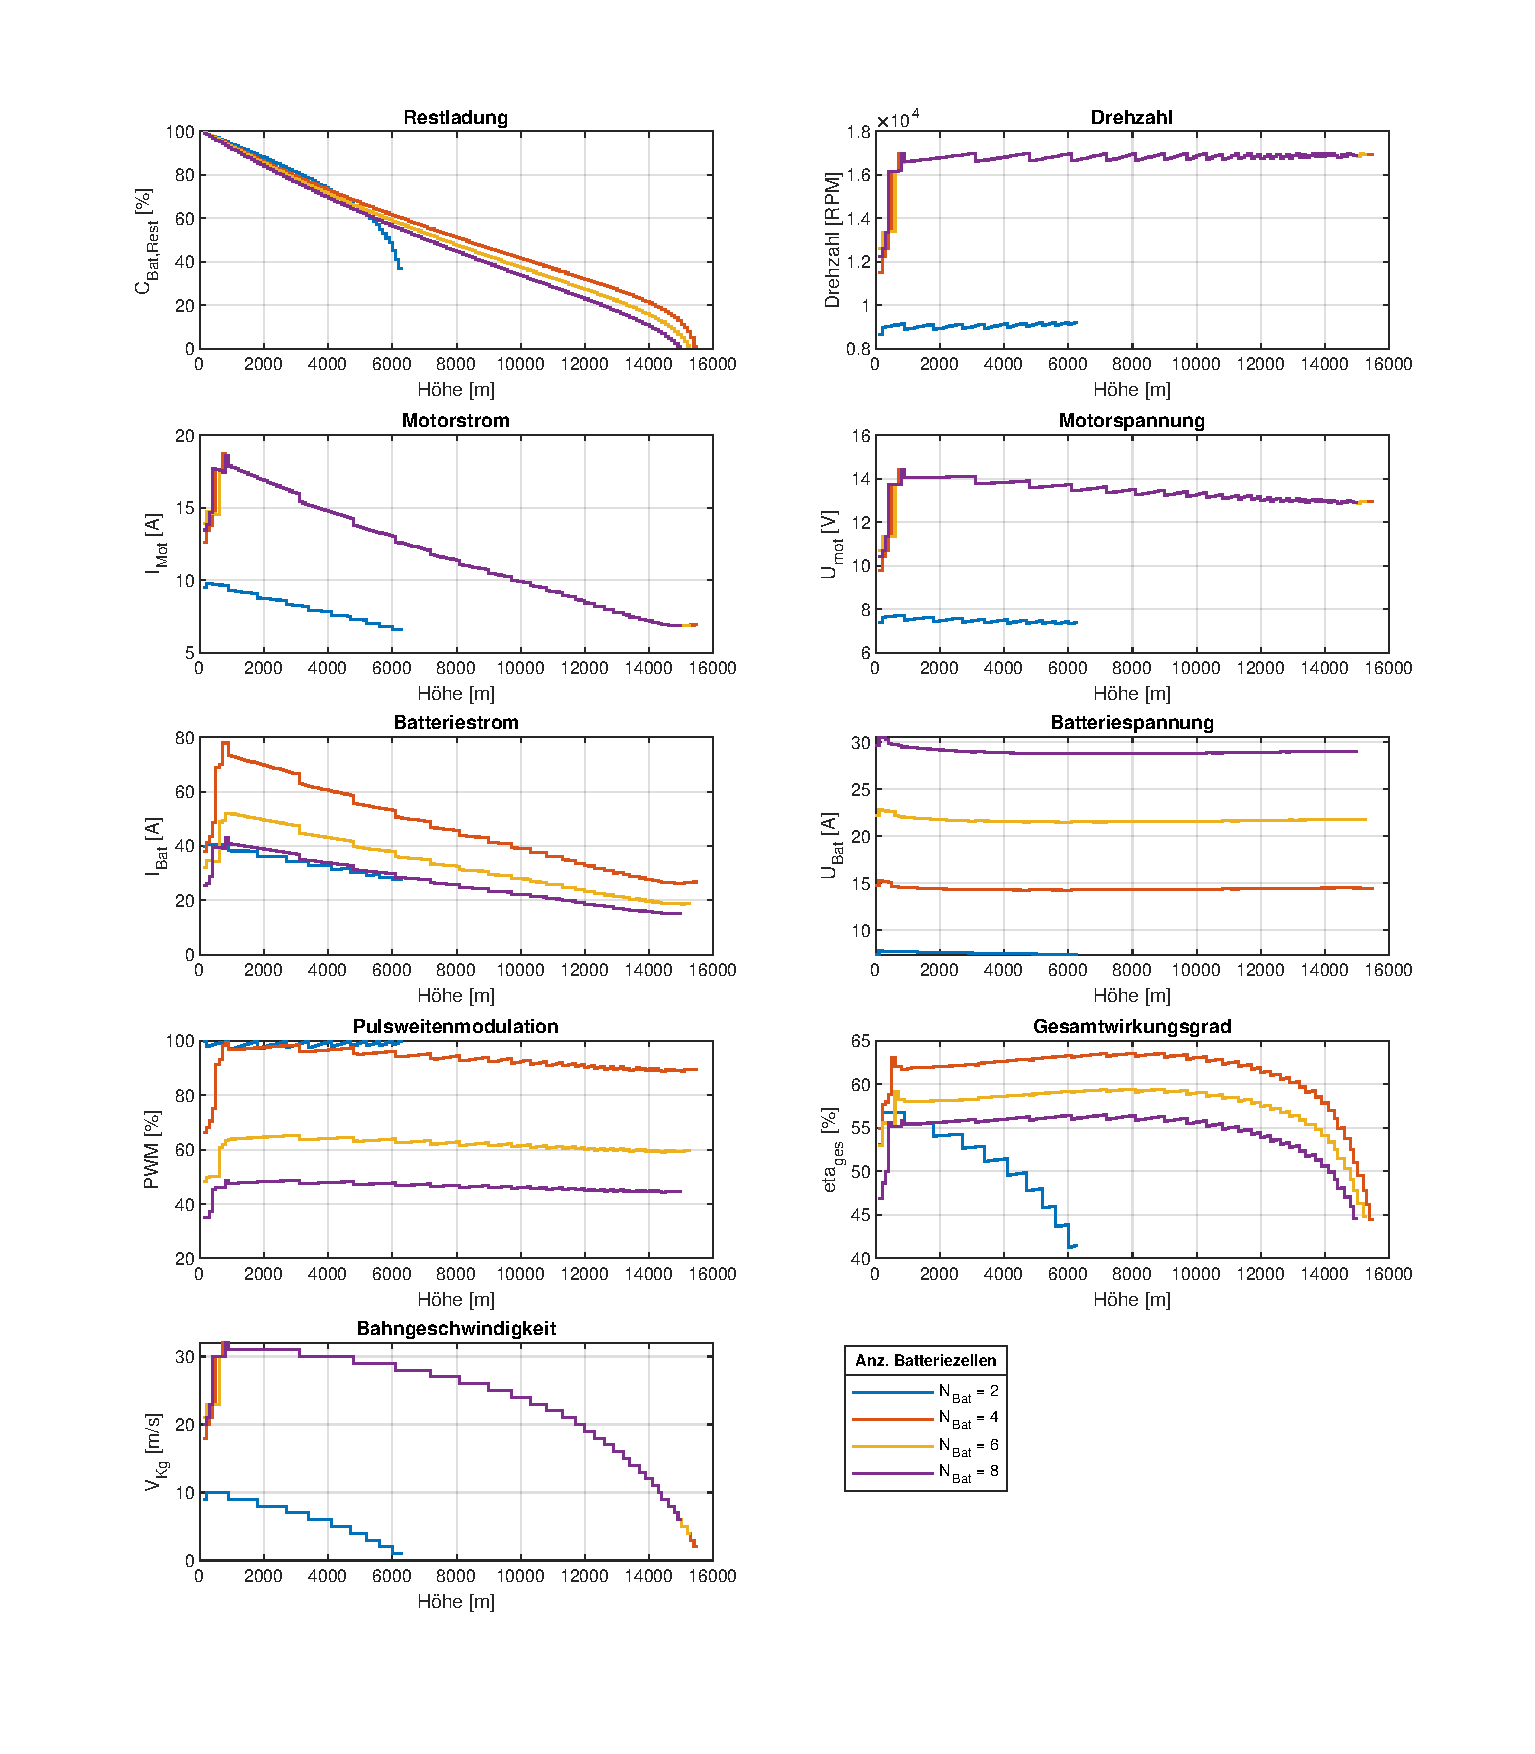
\includegraphics[scale=0.70]{Diagramme/Untersuchung_N_Bat.pdf}
	\caption{Einfluss des Batteriezellenanzahl auf die Flugleistungen der Multicopter-Referenzkonfiguration (Tab. \ref{tab:referenzkonfiguration_mulitcopter})}
	\label{abb:N_Bat_einfluss}
\end{figure}


\subsection{Einfluss des Motorreglerwirkungsgrades}
\label{subsec:einfluss_eta_pwm}
Der Wirkungsgrad des ESC ist ausschließlich als eine Funktion der PWM modelliert (vgl. Gleichung \eqref{eq:eta_pwm}). Wie bereits in Abschn. \ref{subsec:einfluss_n_bat} erklärt, sinkt die PWM mit der Erhöhung der Batteriezellenanzahl. Zeitgleich steigen die Verluste im Motorregler. Im Sinne eines besseren Gesamtwirkungsgrades und der erreichbaren Höhe ist eine Verringerung der Motorreglerverluste anzustreben. Die Ergebnisse sind in \ref{sec:motorreglerwirkungsgrad} dargelegt. \\
Der Motorreglerwirkungsgrad hat keinen Einfluss auf die Dienstgipfelhöhe. Es ist allerdings ein bedeutender Einfluss auf die Restladung zu erkennen. Mit einem höheren ESC-Wirtkungsgrad steigt auch der Gesamtwirkungsgrad. Weiterhin sinkt der Batteriestrom (vgl. Gleichung \eqref{eq:batteriestrom}) mit dem Reglerwirkungsgrad und über den geringeren Batteriestrom sinkt die der Batterie entnommene Kapazität. Werden die Kurven der Restladung linear extrapoliert, so würde die Konfiguration mit sechs Zellen und bei einer Halbierung der Verluste im Motorregler ohne die Dienstgipfelhöhe bereits \SI{18000}{m} und mit keinen Verlusten im Regler bereits mehr als \SI{20000}{m} Höhe erreichen. \\
Daher sind aus den oben genannten Gründen die Verluste innerhalb des Motorreglers zu verringern. 


\subsection{Einfluss des maximalen Motorstroms}
\label{subsec:einfluss_imax}
Die Ergebnisse zeigen, dass ein geringer maximaler Motorstrom ebenfalls die Bahngeschwindigkeit begrenzt (vgl. z.B. Abb. \ref{abb:c_W_einfluss}). Dieser begrenzt die dem Motor entnommene Leistung. 
Folglich ist ein Motor für einen solchen Steigflug zu wählen, der einerseits einen hohen \ensuremath{K_V}-Wert besitzt, andererseits aber auch einen hohen maximalen Dauerstrom besitzt (vgl. Kap. \ref{subsec:mot_prop_kombi}). Ein gutes Beispiel ist der Motor aus Kapitel \ref{sec:flaechenflugzeug_referenzkonfig} mit einem \ensuremath{K_V}-Wert von \SI{1390}{RPM/V} und einem maximalen Motorstrom \ensuremath{I_{max}} von \SI{35}{A}.



%******************************************************************

\subsection{Massenanteile der Komponenten}
\label{subsec:massenverteilung}
Ein weiterer wichtiger Punkt, der an dieser Stelle untersucht werden soll, ist die Massenanteilsverteilung von den Motoren, der Batterie und der Leermasse des Multicopters am Gesamtgewicht. Wiederum stellt der Quadrocopter aus Kapitel \ref{chap:nachbildung_des_quadrocopter} die Grundlage der Untersuchung dar. Bei diesem nehmen die Motoren \SI{13,77}{\%}, die Batterie \SI{52,83}{\%} und der Rahmen mit den übrigen Komponenten \SI{33,4}{\%} der Gesamtmasse von \SI{1060}{g} ein. Diese Massenverhältnisse sind bereits bei der Multicopter-Referenzkonfiguration angewendet worden (vgl. Kap. \ref{sec:multicopter_referenzkonfig}). Zusätzlich wurde auch die obere Stirnfläche \ensuremath{F_{copter,oben}} mit der Größe angepasst. Für die genauere Betrachtung der optimalen Massenverteilung wird die Batteriemasse im Verhältnis zur Gesamtmasse variiert.

\begin{figure}[H]
\centering
	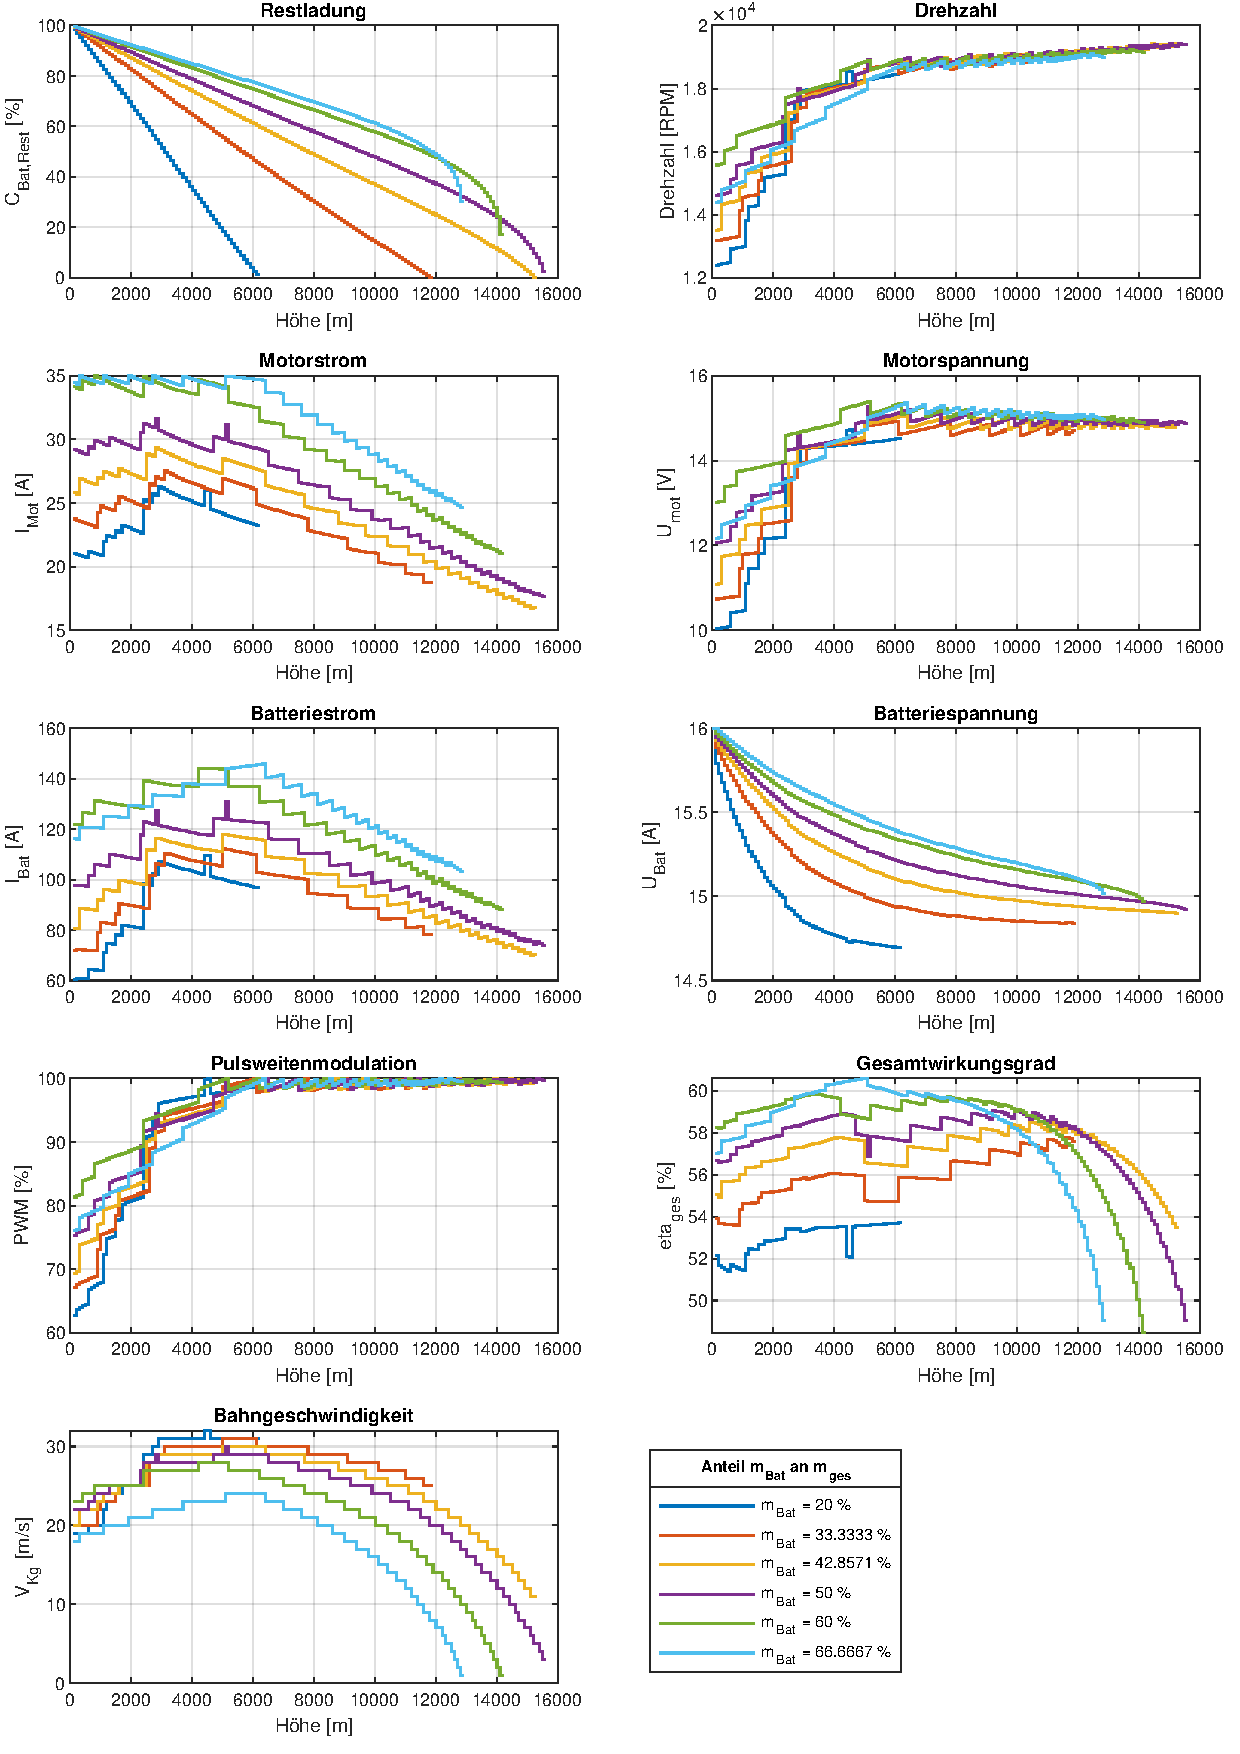
\includegraphics[scale=0.70]{Diagramme/Batteriemasse.pdf}
	\caption{Einfluss des Batteriemassenanteils auf die Flugleistungen der Multicopter-Referenzkonfiguration (Tab. \ref{tab:referenzkonfiguration_mulitcopter})}
	\label{abb:batteriemasse}
\end{figure}

Der Einfluss der Batteriemasse auf die Flugleistungen ist bedeutend (vgl. Abb. \ref{abb:batteriemasse}). Die TOCs variieren in eine Spanne von \SI{5000}{m}. Hier kommt es zu einer Überlagerung zweier Effekte. Der erste ist der Einfluss der Batteriezellenanzahl, der bereits in Abschn. \ref{subsec:einfluss_n_bat} genauer erklärt wurde, und der zweite ist der Einfluss der Batteriemasse. \\
Es kann festgehalten werden, dass mit der Batteriemasse die Batteriekapazität steigt (vgl. Gleichung \eqref{eq:batteriekapazitaet}). Die zur Verfügung stehende Energie erhöht sich. Außerdem erhöht eine höhere Batteriemasse die Gesamtmasse (vgl. Gleichung \eqref{eq:masse_multicopter}) und als Konsequenz auch den erforderlichen Propellerschub (vgl. Gleichung \eqref{eq:neigungswinkel} und \eqref{eq:schub_multicopter}). Diesem folgt eine Erhöhung des Motor- (vgl. Gleichung \eqref{eq:motorstrom}) und des Batteriestroms (vgl. \eqref{eq:batteriestrom}).
Bei Batteriemassenanteilen von weniger als \SI{33,33}{\%}, also einem Drittel der Gesamtmasse, limitiert die Batteriekapazität den Steigflug. Durch die geringe Masse werden die Motoren nicht vollständig ausgelastet, sodass der Motorstrom mit dem Drehmoment des Propellers kontinuierlich ansteigt (vgl. Gleichung \eqref{eq:motorstrom}). Der Drehzahlzuwachs ist zudem signifikant größer als bei höheren Batteriemassenanteilen. Entsprechend steigt auch die Motorspannung an (vgl. Gleichung \eqref{eq:motorspannung}). Der Batteriestrom nimmt äquivalent zum Motorstrom und -spannung zu (vgl. Gleichung \eqref{eq:batteriestrom}).
Zudem ist ein stärkerer Spannungseinbruch zu verzeichnen, je kleiner der Batteriemassenanteil ist. Eine Erklärung liefert die Entladerate, die sich aus dem Batteriestrom in Abhängigkeit der Kapazität zusammensetzt und für eine geringere Kapazität steigt (vgl. Gleichung \eqref{eq:c_rate}). Die Bahngeschwindigkeit ist jedoch am höchsten und sinkt mit höherem Gesamtgewicht, weil der Schub und letztlich die notwendige Energie mit dem Gewicht und der Bahngeschwindigkeit steigen. Weiterhin kann die Dienstgipfelhöhe durch die Motorleistung nicht erreicht werden. Bei sehr kleinen Batterien reicht hierzu die Kapazität nicht aus. Deshalb kann der volle Leistungsüberschuss nicht genutzt werden. \\
Anders ist dies, wenn die Batterie die Hälfte der Gesamtmasse ausmacht. Auch hier limitiert die Batteriekapazität die Flughöhe. Jedoch ist die absolute Kapazität bedeutend höher, weshalb auch die maximale Flughöhe höher ist. Wiederum kann der Einfluss der Batteriezellenanzahl auf Batterien mit der gleichen Masse und Kapazität beobachtet werden. Dieser Zusammenhang wird in Abschn. \ref{subsec:einfluss_n_bat} genauer beschrieben. Ab dieser Batteriemasse ist wieder ein effizienter Flug mit maximalen Motorstrom möglich. Je nach der Batteriezellenanzahl ändert sich auch die Dienstgipfelhöhe. Bei \ensuremath{n_{Bat,cell} = 6} ist dies wiederum durch die maximale Propellerdrehzahl begrenzt und bei \ensuremath{n_{Bat,cell} = 4} limitiert die PWM die Motorleistung, sodass der Schubüberschuss aufgebraucht ist. Die Abhängigkeit der Flugleistungen von der Batteriezellenanzahl zeigt auch die Batterie mit einem Massenanteil von \ensuremath{2/3} an der Gesamtmasse. Hier ist die Batteriekapazität wieder größer. Dies verdeutlicht sich in der nochmals geringeren Batteriekapazitätsabnahme. Mit der Masse sinkt auch die Propellerdrehzahl. Durch die größere Gesamtmasse steigt der benötigte Standschub (vgl. Gleichung \eqref{eq:neigungswinkel} und \eqref{eq:schub_multicopter}) und damit sinkt die optimale Bahngeschwindigkeit.
%, weil die Bahngeschwindigkeit mit dem Widerstand erhöht (vgl. Gleichung \eqref{eq:widerstand}).
Zum Schluss steigert der Batteriemassenanteil noch den Gesamtwirkungsgrad. 
Ein Optimum des Batteriemassenanteils liegt bei \SI{66,667}{\%} der Gesamtmasse (vgl. Anhang \ref{sec:batteriemasse}). Dabei ist vor allem noch die Anzahl der Batteriezellen zu berücksichtigen. Im Hinblick auf Abschn. \ref{subsec:einfluss_n_bat} ist die Zellenanzahl auf den Motor anzupassen, sodass die Motorleistung die maximale Höhe nicht begrenzt, wobei der Motorregler verlustarm arbeiten sollte. Auf der anderen Seite sollte die nominelle Batteriespannung nicht so hoch sein, dass die PWM zum Schutz des Motors abgeriegelt werden muss (vgl. Abschn. \ref{subsec:einfluss_n_bat}). 
Der hier ermittelte optimale Batteriemassenanteil stimmt mit den Aussagen von Neitzke überein \cite{Neitzke.2013}.
Es ist außerdem ersichtlich, dass die Flugleistung und -dauer noch weiter verbessert werden können, wenn der Massenanteil des Rahmens und aller übriger Komponenten kleiner wird und die Masse der Batterie im Gegensatz steigt, d.h. eine Tendenz der Multicopterleermasse gegen Null (\ensuremath{m_{Copter}\rightarrow 0} und \ensuremath{m_{Bat}\rightarrow (m_{Bat}+m_{Copter})}).


%******************************************************************
\subsection{Einfluss der Größe}
\label{subsec:groesse}
Ein weitere Einfluss auf die Flugleistungen stellt das Gesamtgewicht des Fluggerätes dar. Dabei wird das Fluggerät äquivalent skaliert. Dies bedeutet, dass die Massenverhältnisse von Motoren, Batterien und die Leermasse im Verhältnis zum Gesamtgewicht konstant bleiben. Das Verhältnis orientiert sich an der Massenverteilung aus Kapitel \ref{subsec:massenverteilung}. Dieses Verhältnis wird für jede Größenskalierung gewahrt. Als Anhaltspunkt dient wieder die Motormasse. Die Propellerauswahl findet nach den Herstellerempfehlungen und eigenen Versuchen statt. Alle anderen Massenverteilungen ergeben sich im Anschluss aus der Motormasse analog zu Kapitel \ref{subsec:massenverteilung}.

\begin{figure}[H]
%\centering
	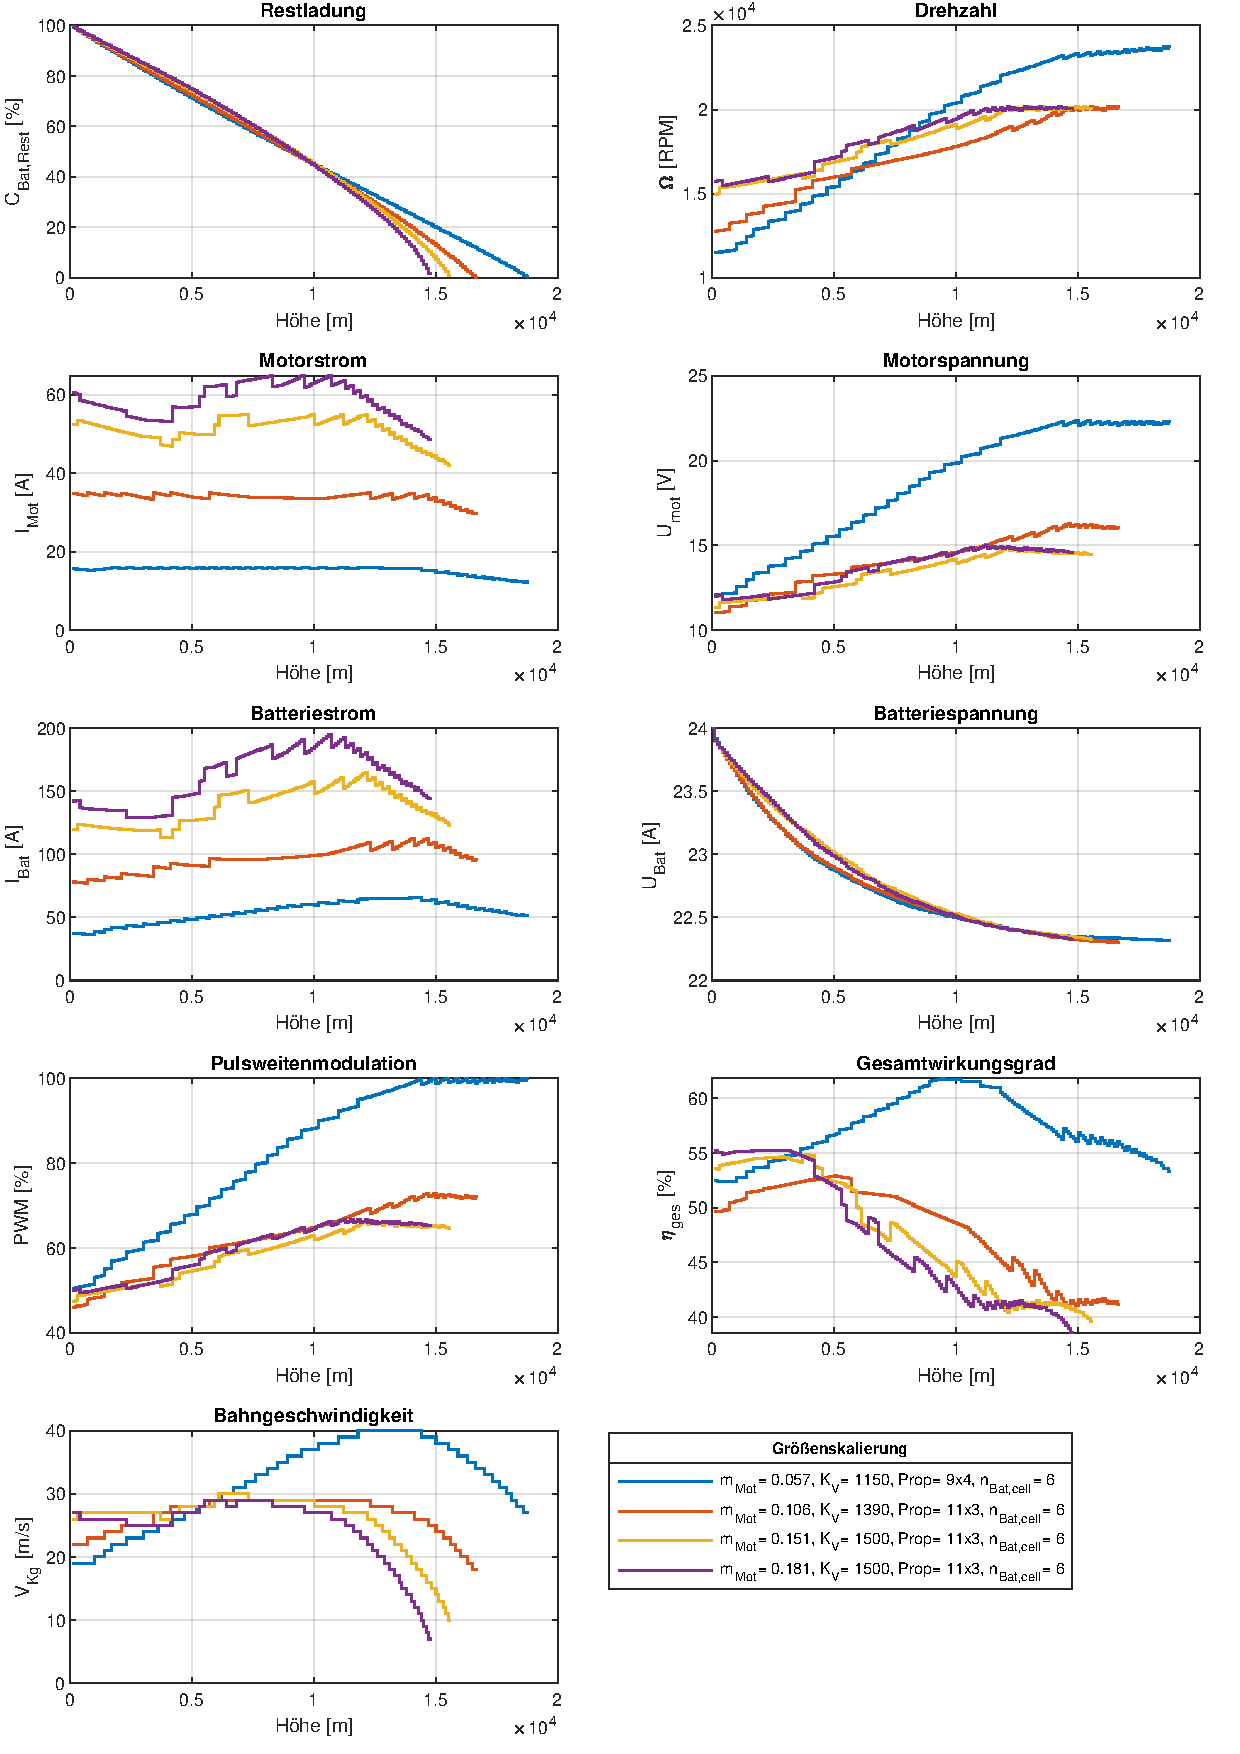
\includegraphics[scale=0.7]{Diagramme/Groessenskalierung.pdf}
	\caption{Einfluss der äquivalenten Größenveränderung auf die Flugleistungen der Multicopter-Referenzkonfiguration (Tab. \ref{tab:referenzkonfiguration_mulitcopter})}
	\label{abb:groessenskalierung}
\end{figure}
Eine äquivalente Größenskalierung besitzt einen vernachlässigbar kleinen Einfluss auf die Flugleistungen (vgl. Abb. \ref{abb:groessenskalierung}). Die Abnahme der Restladung ist für alle Konstellationen beinahe identisch. Der Grund für die Unterschiede in den Diagrammen, die vor allem die Höhe betreffen, liegt in den Unterschieden der Motoren und Propeller. Eine vollständige, uniforme Skalierung ist hier nicht möglich. Dabei unterscheiden sich besonders die \ensuremath{K_V}-Werte der Motoren. Dies zieht Unterschiede im Bereich der Motorspannung und folglich in der PWM und im Gesamtwirkungsgrad nach sich. \\
An dieser Stelle kann somit festgehalten werden, dass eine Größenskalierung keinen Einfluss auf die Flugleistungen hat. Die Vorteile einer größeren Masse liegen für reale Anwendungsfälle vorrangig in der Massenträgheit. In einem Höhensektor von \SI{0}{m} bis \SI{15000}{m} treten im Durchschnitt \SI{100}{km/h} starke Winde auf \cite{Seidel.2011}. Die Einflüsse von Böen in diesen Größenordnungen auf einen Multicopter fallen geringer aus, wenn das Fluggerätes auf eine höhere Gesamtmasse ausgelegt wird. Dies erfordert im Umkehrschluss weniger Energie zur Kurs- und Lagekorrektur. \\
Im Hinblick auf die angedachte Nutzlast von \SI{250}{g} im Rahmen des AEROMET\_UAV-Projektes bietet eine größere Gesamtmasse den Vorteil, dass die feste Masse der Nutzlast anteilig an der Gesamtmasse weniger wird, je größer die Gesamtmasse ist.


\subsection{Anzahl der Propeller}
\label{subsec:anz_prop}
% Wie sich in Abschn. \ref{subsubsec:groesse} zeigte, hat eine uniforme Skalierung des Fluggerätes keinen Einfluss auf dessen Flugleistung. 
Bisher wurden nur Fluggeräte mit vier Rotoren untersucht. Dabei gilt es noch die Abhängigkeit der Flugleistungen von der Propelleranzahl zu überprüfen. 

\begin{figure}[H]
%\centering
	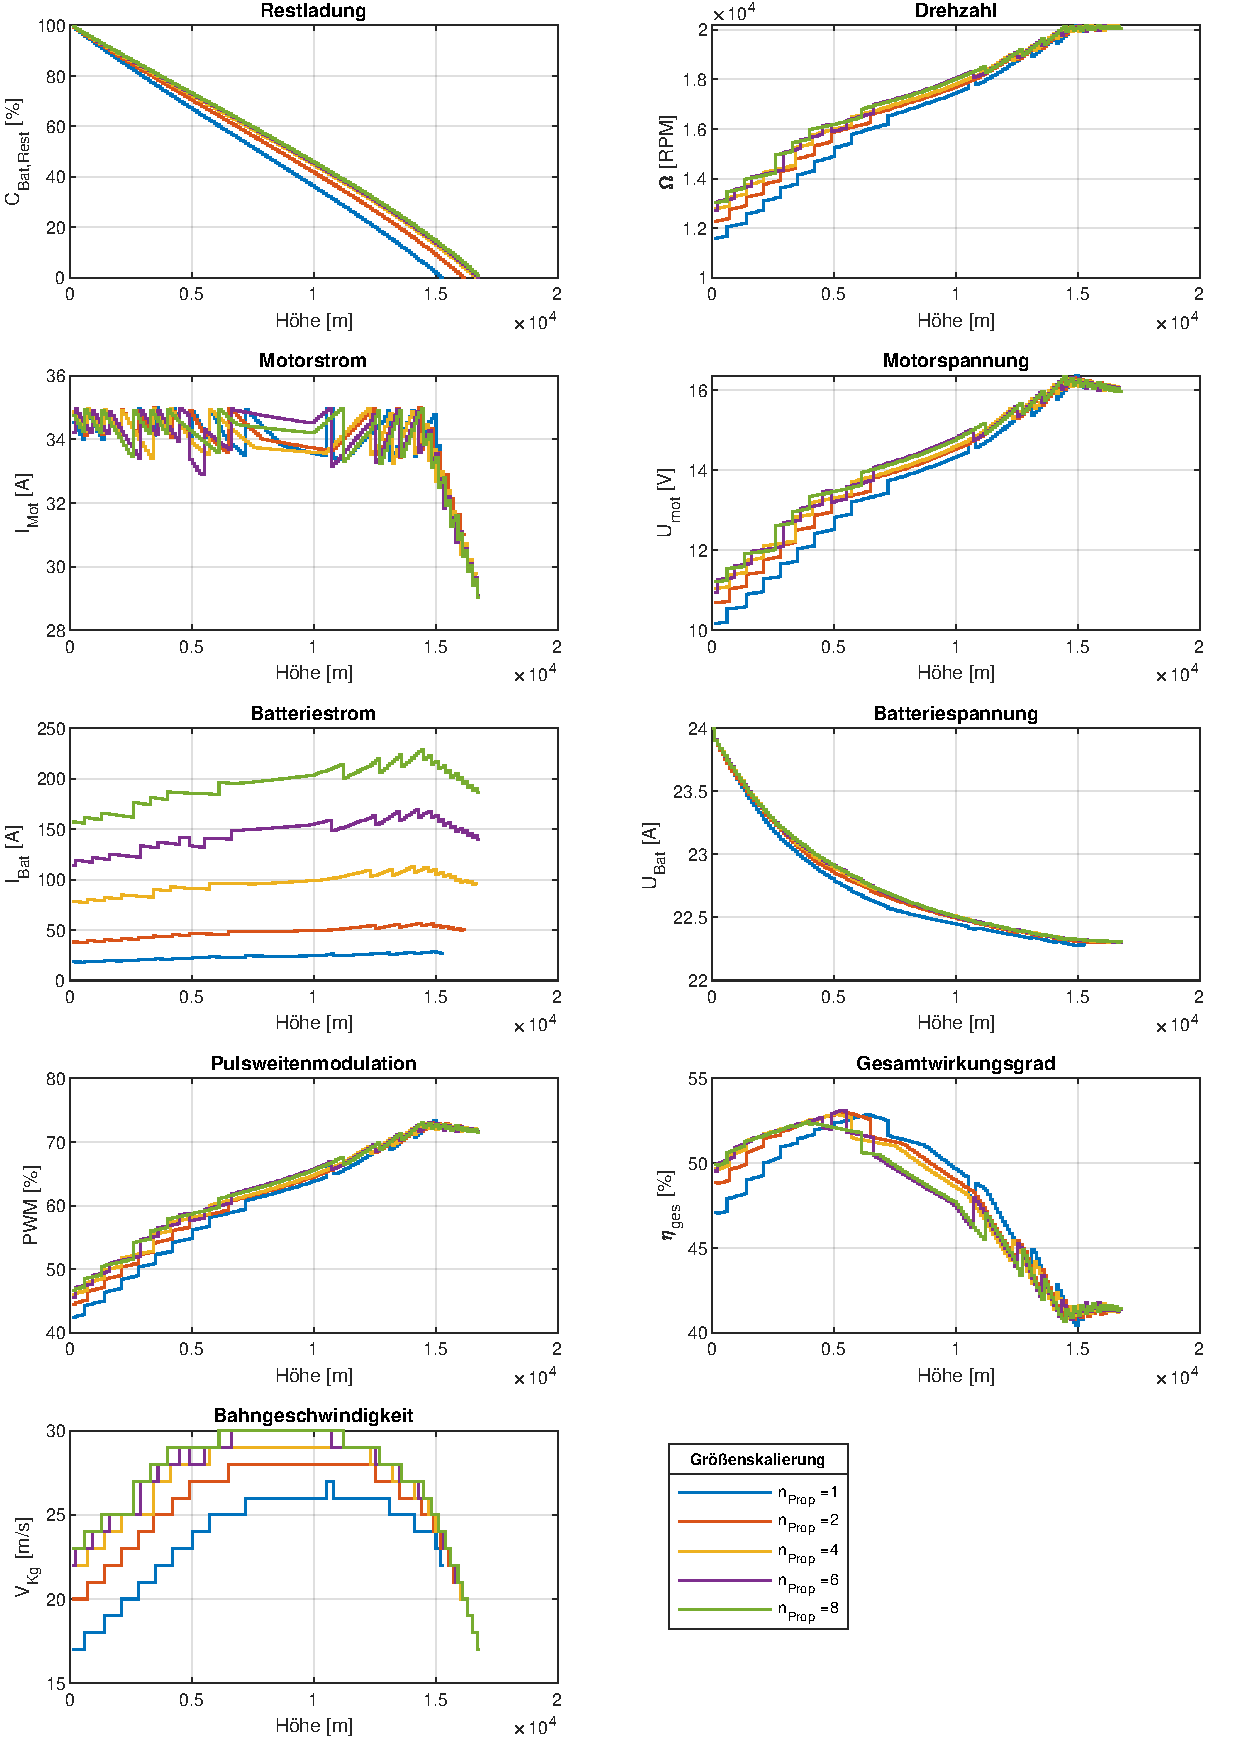
\includegraphics[scale=0.7]{Diagramme/Anz_Prop.pdf}
	\caption{Einfluss der Propelleranzahl auf die Flugleistungen der Multicopter-Referenzkonfiguration (Tab. \ref{tab:referenzkonfiguration_mulitcopter})}
	\label{abb:groessenskalierung}
\end{figure}
Analog zu den Ergebnissen aus Abschn. \ref{subsec:groesse} bewirkt eine äquivalente Veränderung der Rotoranzahl keine nennenswerten Änderungen der maximalen Flughöhe, wenn die verwendeten Motoren dieselben sind. Die Ergebnisse für einen Multicopter mit vier, sechs oder acht Propellern sind nahezu identisch. Dies gilt auch für die Restladung, die für diese Konfigurationen im Vergleich zu den Konfigurationen mit weniger Propellern noch pro Höhenschritt mehr Restladung aufweisen. Die einzigen Unterschiede weisen der Batteriestrom und die Bahngeschwindigkeit auf. Der Batteriestrom erhöht sich mit beinahe konstanten \SI{50}{A} pro zusätzlichen zwei Propellern (vgl. Gleichung \eqref{eq:batteriestrom}). Dahingegen steigt auch die Bahngeschwindigkeit mit mehr Propellern. \\
An dieser Stelle sind jedoch Einschränkungen vorzunehmen. 
Der Monocopter erreicht ähnliche Flugleistungen wie die anderen Konfigurationen. Der Monocopter benötigt jedoch zusätzlich noch Aktuatorik für die Abdeckung der restlichen drei Stellgrößen. Das umfasst Aktuatorik für das Nicken, Rollen und Gieren. Die translatorische Fortbewegung kann bereits durch den Propeller erfolgen. Der Drehmomentenausgleich könnte durch eine der drei rotatorischen Stellgrößen erfolgen (z.B. Rollen). Insgesamt sind also mindestens drei weitere Aktuatoren notwendig. Diese zusätzliche Aktuatorik benötigt der Duocopter ebenfalls. Ein Drehmomentenausgleich ist hier jedoch nicht notwendig. Trotzdem sind hier immerhin noch zwei weitere Aktuatoren für das Nicken und Gieren erforderlich. 
Beide erwähnten Punkte erhöhen die Gesamtmasse und benötigen zusätzlich Energie. Dies verringert die Gesamthöhe. 
Für mehr als vier Propeller muss berücksichtigt werden, dass die Gesamtmasse und damit insbesondere das Strukturgewicht steigt. Dies geht auf die Kosten einer optimalen Konstellation der Massenverteilung. Zusätzlich erhöht sich die obere Stirnfläche \ensuremath{F_{copter,oben}} durch stärkere Strukturen, die in einer Widerstandserhöhung und somit erhöhten Verlusten resultieren. 
Für den anschließenden Sinkflug wäre ein um die Gierachse eigenstabiler und um die Roll- und Nickachse mit den zusätzlichen zwei Aktuatoren steuerbarer Duocopter, welcher die beiden Antriebe abschaltet und sich somit im Gleichtflug befindet, womöglich sehr effizient. Diese Art der Konfiguration spricht für einen Gleitflüger, der die beiden genannten Eigenschaften verbindet.
Um das oben gesagte zusammenzufassen, eignet sich eine Propelleranzahl von mindestens zwei am besten für einen Flug in die untere Stratosphäre. \\


\subsection{Einfluss eines Verstellpropellers}
\label{subsec:verstellprop}
Eine bisherige Begrenzung der Flugleistungen erfolgte häufig durch die maximale Drehzahl des Propellers, die indirekt die Motorspannung beeinflusst (vgl. Abschn. \ref{subsec:widerstandseinfluss}). 
Besonders auffällig bei vorherigen Untersuchungen (vor allem in Bezug auf die Untersuchungen des Quadrocopters aus Kap. \ref{chap:nachbildung_des_quadrocopter}) ist, dass die Drehzahl von Propellern mit einer geringen Steigung deutlich schneller steigt als bei einem Propeller mit einer großen Steigung. Da vor allem die Drehzahl die Motorspannung bestimmt, ist eine Verringerung der Drehzahl bei gleichem Schub von Interesse. Mit zunehmender Flughöhe verringert sich die Dichte und dementsprechend auch der Schub, wenn die Rotordrehzahl und die Propellersteigung konstant gehalten werden. Diesem Effekt kann mit einer Erhöhung der Drehzahl oder mit einer Erhöhung der Steigung entgegen gewirkt werden. Während bei einem Drehflügler mit Strahltriebwerk nur eine Blattverstellung, nicht aber eine Drehzahlveränderung möglich ist, besitzen elektrische, propellergetriebene Fluggeräte beide Möglichkeiten. Dies kann mit einem Verstellpropeller und entsprechender Aktuatorik realisiert werden. \\
Im Rahmen dieser Untersuchung liegen nur Propellerkennfelder mit einer konstanten Propellersteigung vor. Das Vorgehen für einen Propeller mit variabler Steigung sieht so aus, dass für einen vorgegebenen Durchmesser alle Kennfelder mit diesem Durchmesser der Datenbank entnommen werden (siehe \ref{sec:vprop_vorgehen}). Danach wird in der Leistungsuntersuchung jeder Propeller mit unterschiedlicher Steigung, aber gleichem Durchmesser, gegeneinander abgewogen. Die Auswahl für den in dem betrachteten Flugmoment beste Steigung erfolgt wieder über die Energiebetrachtung analog zum Bahnneigungswinkel und der Bahngeschwindigkeit (vgl. Kap. \ref{subsubsec:schub_flaechenflzg}). Dies ist ein Idealfall, weil mit der minimal aufgebrachten Energie auch die der Batterie entzogenen Restladung minimal ist. Folglich wird nur der Zustand ausgewählt, der die größte Restladung aufweist.

\begin{figure}[H]
\centering
	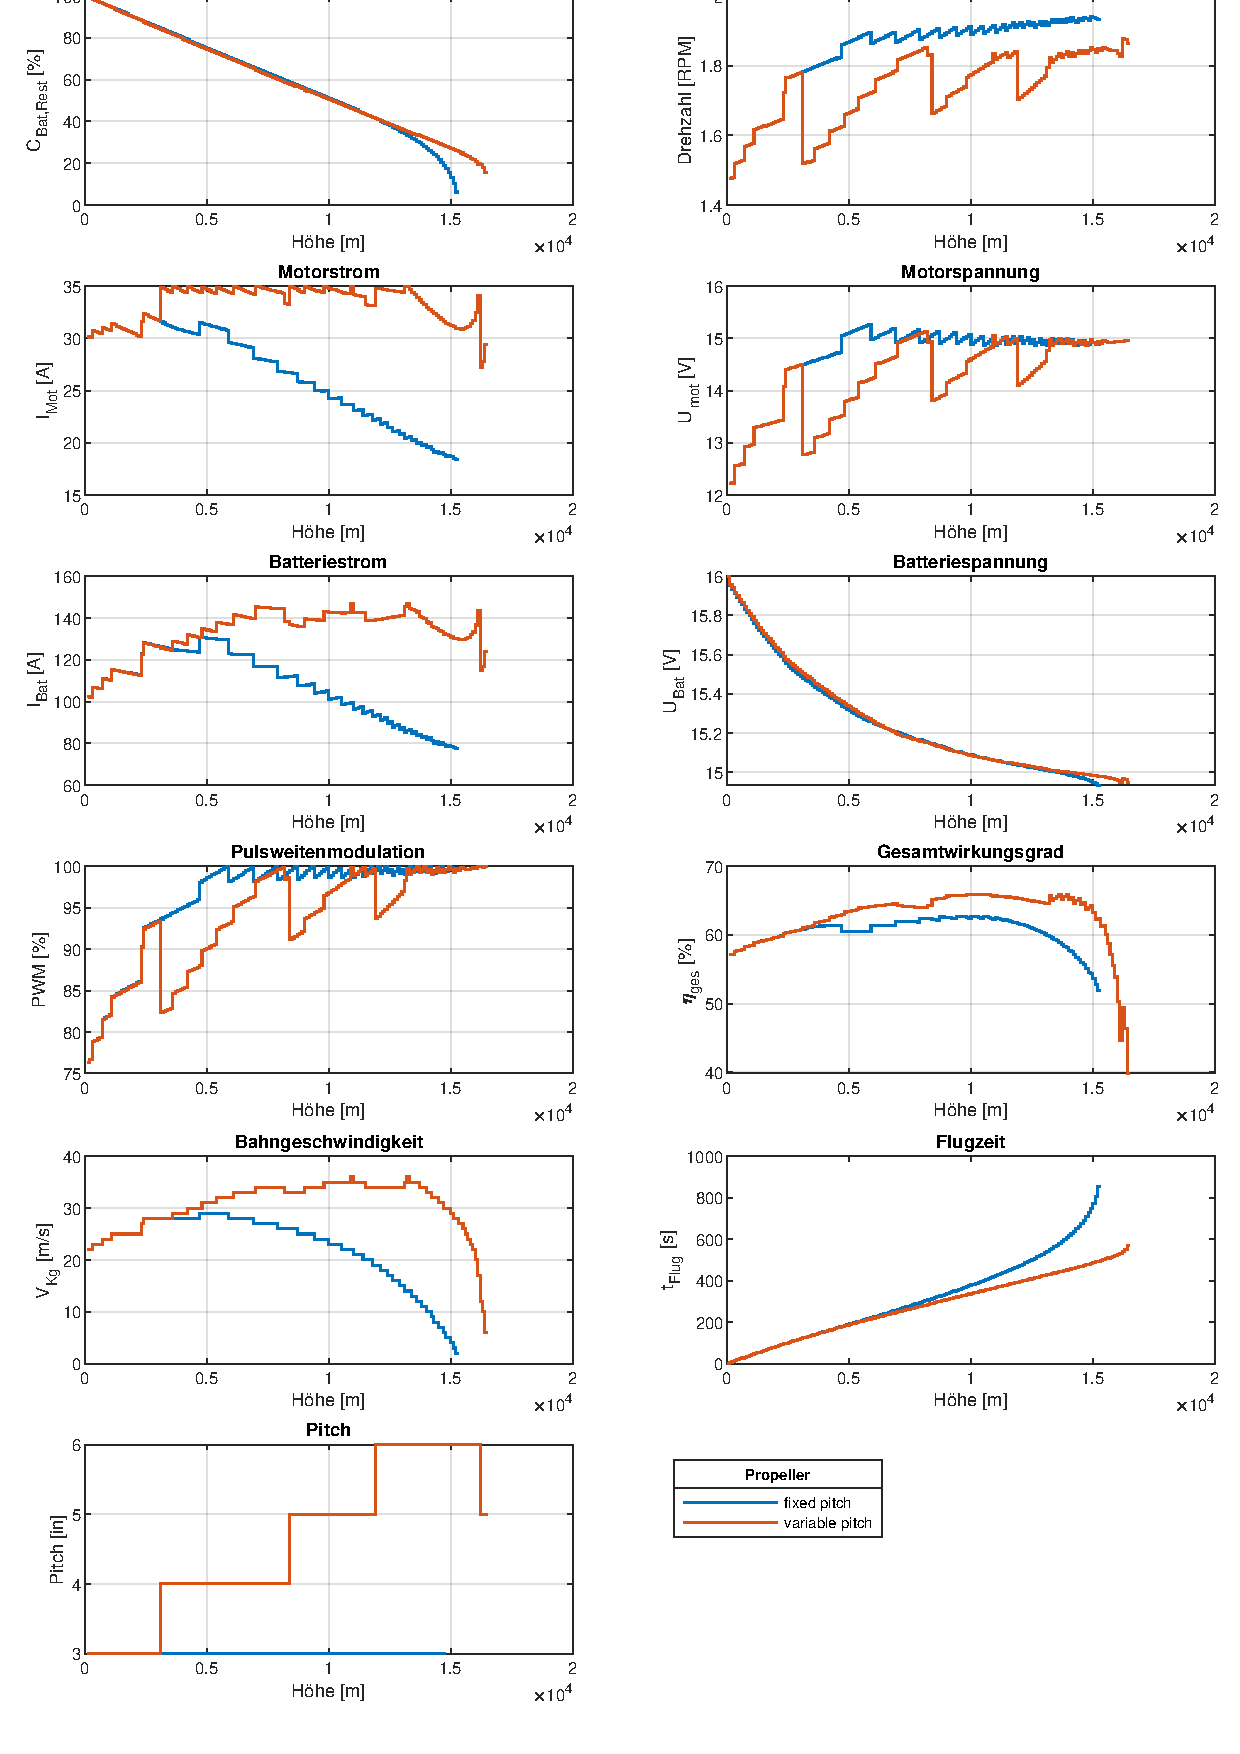
\includegraphics[scale=0.7]{Diagramme/Verstellpropeller.pdf}
	\caption{Einfluss eines idealen (Eigengewicht gleich null und ideale Verwindung) Verstellpropellers auf die Multicopter-Referenzkonfiguration (Tab. \ref{tab:referenzkonfiguration_mulitcopter})}
	\label{abb:verstellpropeller}
\end{figure}
Mit dem Verstellpropeller ist ein deutlicher Höhengewinn von \SI{2000}{m} zu verzeichnen. Selbst mit dem Verstellpropeller wird ab \SI{17500}{m} die Dienstgipfelhöhe erreicht, die sich wieder durch die Begrenzung der Propellerdrehzahl auszeichnet. Ab \SI{17000}{m} ist die Blattspitzengeschwindigkeit  \ensuremath{Ma_{tip} = 1}. Allerdings sind die Auswirkungen auf die Flugleistungen marginal. Hieraus kann geschlossen werden, dass ein Verstellpropeller die Dienstgipfelhöhe in größere Höhen verschieben kann. \\
Mit dem Verstellpropeller kann durchgehend am effizientesten bei maximalen Motorstrom (hier \ensuremath{I_{max} = \SI{35}{A}}) geflogen werden. Die Propellersteigung wächst im Laufe des Steigfluges von anfänglichen \SI{3}{in} auf \SI{5}{in}. Dies ist erstaunlich, da noch viel größere Steigungen möglich wären, die aber selbst in großen Flughöhen immer noch mehr Energie der Batterie entziehen als kleinere Steigungen. Es gilt also, dass geringe Propellersteigungen für Multicopter am effizientesten mit Hinblick auf den Energieverbrauch sind. Die Fluggeschwindigkeit ist allerdings auch gering, sodass sich hohe Steigungen tendenziell erst bei hohen Fluggeschwindigkeiten lohnen. \\
Signifikant ist der Einfluss einer Propellersteigungsänderung auf die Propellerdrehzahl. Aufgrund der Tatsache, dass der Verstellpropeller mit Kennfeldern von Propellern modelliert wird, die eine feste Steigung besitzen, bedeutet eine Änderung der Propellersteigung auch eine Änderung der Drehzahl. Diese Drehzahleinbrüche treten auf, da ein Propeller mit einer höheren Steigung denselben Schub bei einer geringeren Drehzahl erzeugen kann. Der Verlauf der Drehzahl wirkt sich direkt auf die Motorspannung aus (vgl. Gleichung \eqref{eq:motorspannung}), damit auch auf die PWM (vgl. Gleichung \eqref{eq:pwm}) und letztlich auf den Batteriestrom (vgl. Gleichung \eqref{eq:batteriestrom}). Im Vergleich zum Propeller mit konstanter Steigung ist die PWM durch die vergleichsweise geringere Drehzahl und die geringere Motorspannung unterhalb der PWM der Referenzkonfiguration. Folglich fällt auch der Motorreglerwirkungsgrad schlechter aus. Allerdings wird durch die Propellersteigungsänderung eine deutliche Erhöhung des Propellerwirkungsgrades erzielt. Dies kann auf die langsamer drehenden Propeller, aber deutlich schneller fliegenden Multicopter zurückgeführt werden (vgl. Gleichung \eqref{eq:eta_prop}). Eine Propellersteigungserhöhung liefert gleichzeitig auch mehr Schub. Somit ist auch eine höhere Bahngeschwindigkeit möglich. Insgesamt liegt somit der Gesamtwirkungsgrad \ensuremath{\eta_{ges}} vom Multicopter mit Verstellpropeller ab \SI{7000}{m}, wenn die Propellersteigung das erste Mal erhöht wird, ca. \SI{3}{\%} (mit einer steigenden Tendenz) über dem Multicopter ohne. In \SI{15000}{m} Höhe sind es sogar mehr als \SI{10}{\%}. \\
Eine Änderung auf die Abnahme der Restladung macht sich erst ab ca. \SI{10000}{m} Höhe bemerkbar. Während die Restladung vom Multicopter ohne Verstellpropeller ab dieser Höhe schneller abnimmt, kann sie durch einen Verstellpropeller verlangsamt werden. Dies bedeutet, dass ein Verstellpropeller die Effizienz in niedrigen Höhen nicht bedeutend beeinflusst. Für Steigflüge in großen Höhen kann er jedoch die Effizienz deutlich anheben.
% Dies gilt jedoch nicht bei Steigflügen in noch größere Höhen, da er dort die Effizienz deutlich anhebt.
%Der zusätzliche Höhengewinn durch einen Verstellpropeller liegt bei  ca. \SI{1500}{m} (vgl. Abb \ref{abb:verstellpropeller}). Dabei handelt es sich um einen idealen Verstellpropeller, dessen Verstellmechanismus und -aktuatorik nicht in das Gesamtgewicht einbezogen werden. \\
%Die Leistungsparameter beider Propellerarten sind für die ersten \SI{3000}{m} identisch. Dies liegt an der gleichen Propellersteigung. Danach nimmt die optimale Propellersteigung kontinuierlich zu. Durch die Tatsache, dass die Steigung variabel ist, ist durchgehend ein Flug mit maximaler Motorleistung, d.h. bei einem maximalen Motorstrom und -spannung, möglich. Durch jede Verstellung kommt es zu einem Einbruch der Drehzahl, der sich durch den Verlauf der Motorspannung und der PWM fortpflanzt (entspr. Gleichung \eqref{eq:motorspannung} und \eqref{eq:pwm}). Bis zu einer Höhe von \SI{3000}{m} hat der Verstellpropeller keinen Einfluss auf die Restladung oder die Batteriespannung. Die deutlich höhere Effizienz des Fluges bei maximalen Motorstrom zeigt sich im Gesamtwirkungsgrad. Durch die mit der Propellersteigungsänderung steigende Bahngeschwindigkeit erhöht sich auch der Propellerwirkungsgrad. Daher erhöht sich auch der Gesamtwirkungsgrad. 
%Ein Vorteil, der in Abb. \ref{abb:verstellpropeller} ersichtlich wird, ist, dass durch eine Erhöhung der Propellersteigung der gleiche, wenn nicht sogar noch mehr Schub, bei einer geringeren Drehzahl durch den Propeller erzeugt werden kann. Dies erhöht den Leistungsüberschuss und letztendlich die erreichbaren Fluggeschwindigkeiten bei voller Motorauslastung. Entsprechend sinkt die Flugzeit.
%Bedeutend ist noch zu erwähnen, dass die Restladung am TOC bei einem Multicopter mit Verstellpropeller noch bedeutend höher ist (insg. noch ca. \SI{20}{\%}) als die bei einem ohne. \\
Der Vorteil eines Verstellpropellers ist deutlich. Dazu müssen aber noch folgende Einschränkungen vorgenommen werden. Der Verstellpropeller kann nur im Rahmen der in der APC-Datenbank \cite{apc} vorhanden Propeller modelliert werden. Dies setzt Ungenauigkeiten voraus, da eine kontinuierliche Verstellung nicht nachgebildet werden kann und nur so viele Verstellungen berücksichtigt werden können, wie auch Propeller mit verschiedenen Steigungen in der Datenbank vorhanden sind. Eine kontinuierliche Verstellung würde an dieser Stelle einen glatten Verlauf in der Propellersteigung und somit auch in allen anderen Verläufen erzeugen. \\
An dieser Stelle wurde der Propeller in gewisser Weise idealisiert. So wurde unter anderem die verlängerte Blattaufhängung mit dem Steuerstangenanschluss und der Verstellaktuatorik etc. außer Acht gelassen. Dies würde zu zusätzlichen Verlusten an der Blattwurzel und einer Verringerung des effektiven Radius führen. Bei einem Propeller mit konstantem Anstellwinkel kann diese sehr kurz gehalten werden, weshalb das profilierte Rotorblatt radial gesehen deutlich früher beginnt. Die Verringerung der effektiven Propellerblattlänge ist bei dem hier modellierten Verstellpropeller nicht berücksichtigt worden. Weiterhin birgt die Verwendung von Propellerkennfeldern mit einer festen Steigung gewisse Ungenauigkeiten. Für die Propeller mit fester Steigung kann vorausgesetzt werden, dass dieser im Rahmen eines optimalen Schwebeflugrotors \cite[S.197-S.205]{Wall.2015} ausgelegt wurde (ausschließlich axiale Anströmung, Betrieb nur im Vorwärtsflug, etc). Ein Verstellpropeller muss jedoch eine gewisse Bandbreite an Betriebspunkten abdecken (Steig-, Vorwärtsflug oder Autorotation), die durch eine einseitige Optimierung des Propellers eine Verschlechterung für die anderen bedeutet \cite[S.203]{Wall.2015}. Es ist daher auch mit Diskrepanzen für das Leistungsverhalten des Verstellpropellers in Bezug auf Propeller mit fester Steigung zu rechnen, die nicht den Kennfeldern zu entnehmen sind. \\
Weiterhin wurden in dieser Betrachtung das Gewicht des Verstellmechanismus an sich und der Aktuatorik für jeden einzelnen Propeller nicht berücksichtigt. Hierbei bedeuten die Aktuatoren zusätzliche Verbraucher für die Batterie, die mitunter deutlich schneller zu einem Flug bei \SI{100}{\%} PWM führen würden. Letztendlich ist der fehlende Schub in großen Höhen nicht das Begrenzungsmerkmal, sondern die Drehzahl des Propellers und Motors sowie die Batteriespannung, kurz der Leistungsüberschuss. Letzterer macht den Verstellpropeller ein weiteres Stück redundant. %(vgl. \ref{abb:vertellprop_real}). 
Mit einem hohen Batteriestrom verschiebt sich der Bereich, in dem ein größere Steigung vorteilhafter ist, noch weiter in größere Höhen. Damit sinkt auch die Einsatzdauer und schließlich der Nutzen. 
Schlussendlich bringt der Verstellpropeller den Vorteil der Autorotation mit, der weniger für den Steigflug als für den anschließenden Sinkflug von Bedeutung ist. Durch die Autorotation ist ein antriebsloser Sinkflug möglich. Damit könnte die Batterie noch weiter entladen werden bevor ein Sinkflug eingeleitet werden muss, was im Umkehrschluss die erreichbare Höhe steigert. Außerdem erhöht ein Verstellpropeller die Restladung am TOC, sodass das volle Potential dieser Propellerart ausgeschöpft werden kann. Im Zustand der Autorotation ist jedoch kein Ausgleich von Seitenwinden möglich. Die Abdrift muss daher an dieser Stelle negativ bewertet werden. \\
Zusammengefasst gilt, dass ein Verstellpropeller Vorteile in großen Höhen mit sich bringt. Allerdings ist die hier in Abb. \ref{abb:verstellpropeller} dargelegte Effizienz anzuzweifeln. Die Vorteile ergeben sich auch in Abhängigkeit der Konstruktion. Je kleiner die Blattaufhängung ist, desto effizienter ist der Verstellpropeller. Weiterhin ist die Masse des Verstellmechanismus im Verhältnis zum Gesamtgewicht abzuwägen. Je größer das Gesamtgewicht des Multicopters, desto geringer ist der nachteilige Einfluss der Zusatzmasse durch den Verstellpropeller auf dessen Flugleistungen. Aus diesem Grund ist der reale Nutzen für kleinere Multicopter zu verneinen. 
In \ref{sec:vprop_vorgehen} werden die Flugleistungen für einen Verstellpropeller mit Eigengewicht dargelegt. 



\subsection{Einfluss eines stufenlosen Getriebes}
\label{subsec:getriebe}
Eine häufige Begrenzung der Leistung ist die maximale Drehzahl des Motors oder des Propellers (vgl. u.a. Abschn. \ref{sec:flaechenflugzeug_referenzkonfig} und \ref{subsec:widerstandseinfluss}). Diese nimmt mit großen Höhen stark zu. Ein hypothetisches, stufenlos verstellbares Getriebe bringt den Vorteile mit, dass durch dessen Einsatz die Drehzahl für den Motor entsprechend angepasst werden kann, sodass die Motorspannung nicht mehr den Flaschenhals für einen Steigflug darstellt.
Die Übersetzung für ein Getriebe 
\begin{equation}
	i = \frac{\Omega_{an}}{\Omega_{ab}} 
	\label{eq:getriebe_uebersetzung}
\end{equation}
setzt sich in Abhängigkeit der Drehzahlen aus dem Verhältnis der Eingangsdrehzahl \ensuremath{\Omega_{an}} zur Ausgangsdrehzahl \ensuremath{\Omega_{ab}} zusammen. Weiterhin gilt für die Leistung, dass unter Berücksichtigung von Verlusten innerhalb des Getriebes die Eingangsleistung \ensuremath{P_{an}} gleich der Ausgangsleistung \ensuremath{P_{ab}} ist
\begin{equation}
	P_{an} = \eta_{Getriebe} \cdot \Omega_{an}\cdot M_{an} = \Omega_{ab}\cdot M_{ab} = P_{ab}
	\label{eq:getriebe_leistung}
\end{equation} 
mit dem Getriebewirkungsgrad 
\begin{equation}
	\eta_{Getriebe} = \frac{P_{ab}}{P_{an}} \leq 1 \eqend{.}
	\label{eq:getriebe_wirkungsgrad}
\end{equation}
Aus den Gleichungen \eqref{eq:getriebe_uebersetzung} bis \eqref{eq:getriebe_wirkungsgrad} ergeben sich nun für die aus dem Propellerkennfeld ermittelten Drehzahl und dem Drehmoment die neue Drehzahl für den Motor
\begin{equation}
	\Omega_{neu} = \Omega_{Kennfeld}\cdot i
\end{equation}
und aus der Leistung
\begin{equation}
	M_{neu} = \frac{P_{ab}}{\Omega_{neu}} \eqend{.}
\end{equation}
das neue Drehmoment.
Die günstigste Übersetzung wird analog zum Steigwinkel des Flächenflugzeuges und analog zur Bahngeschwindigkeit durch eine Iteration über der Übersetzung \ensuremath{i} gefunden (siehe Anhang \ref{sec:getriebe_vorgehen}). Das Entscheidungskriterium ist auch hier die minimal aufgebrachte Energiemenge für den jeweiligen Höhenschritt. An dieser Stelle ist das Getriebegewicht \texttt{m\_Getriebe} nicht zu vernachlässigen. Diese fließt mit der Anzahl der Propeller in die Berechnung der Gesamtmasse mit ein
\begin{equation}
	m = m_{Bat} + (m_{Mot} + m_{Getriebe})\cdot n_{Prop} + m_{Copter} \eqend{.}
\end{equation}

\begin{figure}[H]
\centering
	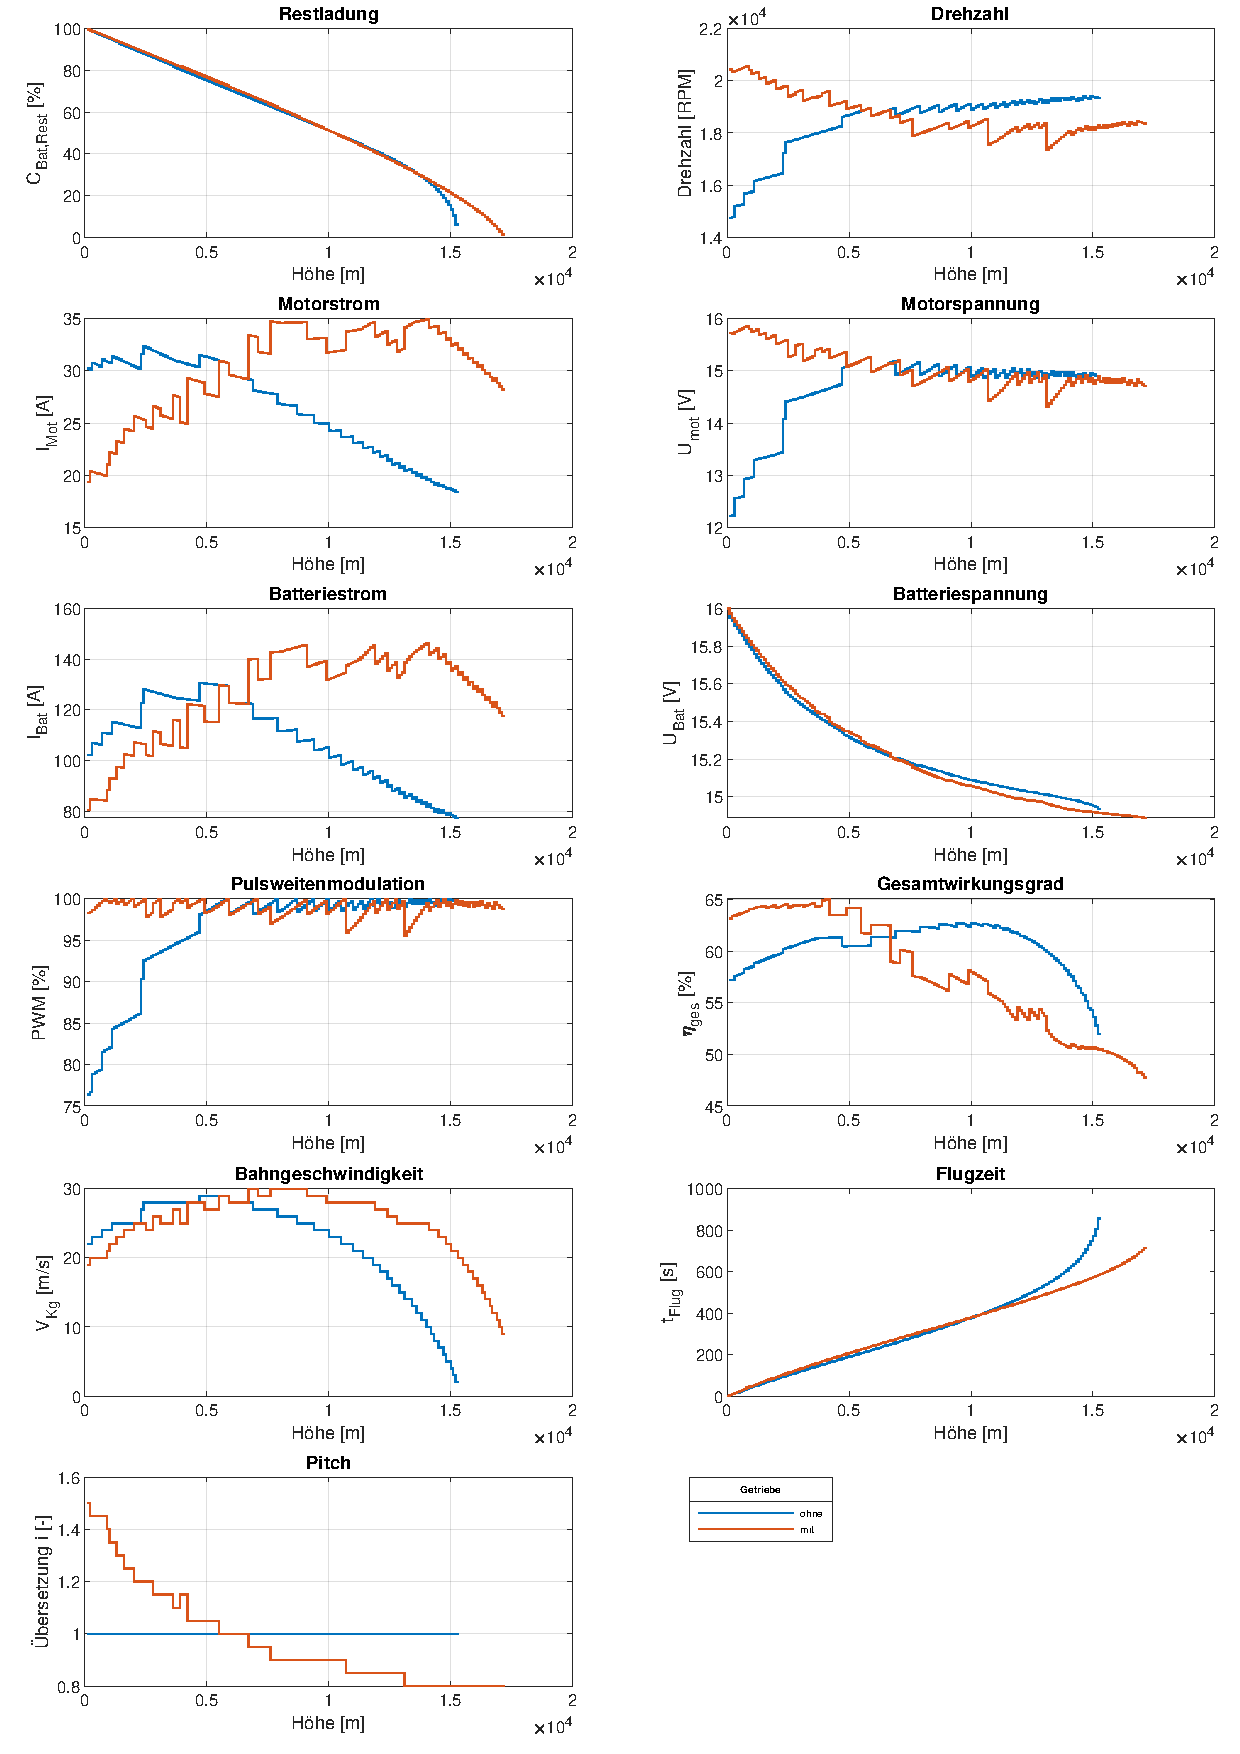
\includegraphics[scale=0.7]{Diagramme/Getriebe.pdf}
	\caption{Einfluss eines idealen (Eigengewicht gleich null und Getriebewirkungsgrad gleich \SI{100}{\%}) Getriebes auf die Flugleistungen der Multicopter-Referenzkonfiguration (Tab. \ref{tab:referenzkonfiguration_mulitcopter})}
	\label{abb:getriebe}
\end{figure}
Der Einsatz eines idealen, stufenlosen Getriebes (\ensuremath{m_{Getriebe} = 0} und \ensuremath{\eta_{Getriebe} = 1}) bietet nur minimale Vorteile (vgl. Abb. \ref{abb:getriebe}). Durch das Getriebe ist die Restladung im Durchschnitt um \SI{2}{\%} größer als ohne. Aus der Reihenfolge des Programms ist die Übersetzung der Drehzahlen und Drehmomente genau umgekehrt. In diesem wird die Drehzahl des Propellers für den Motor angepasst. Mit dieser Blickweise wird die Motordrehzahl zuerst ins Schnelle übersetzt und anschließend ab ca. \SI{15000}{m} Höhe ins Langsame. Auf Grund der Tatsache, dass die Leistung über einem Getriebe konstant bleibt und hier vorerst keine weiteren Verluste berücksichtigt werden, ist der Verlauf des Drehmoments komplementär zu dem Drehzahl, sodass die Beziehung in Gleichung \eqref{eq:getriebe_leistung} erhalten bleibt. \\
Die Übersetzung hat keinen Einfluss auf die Propellerdrehzahl. Diese wird durch Interpolation aus dem Propellerkennfeld bestimmt (vgl. Kap. \ref{subsec:propellerzustand}). Die bemerkbaren Unterschiede in Abb. \ref{abb:getriebe} ergeben sich durch die Diskretisierung der Getriebeübersetzung.
Ähnlich kleine Unterschiede weist auch die Bahngeschwindigkeit auf. Dementsprechend klein sind auch die Unterschiede in der Flugzeit. Das stufenlose Getriebe übersetzt hauptsächlich die Drehzahl des Propellers derart, dass der Motor eine beinahe konstante Spannung erfährt von ca. \SI{17}{V}. Die Motorspannung sinkt dabei leicht mit der Höhe auf \SI{16}{V}. Verantwortlich für die konstante Motorspannung ist die Übersetzung, die beinahe hyperbolisch von anfangs 2 auf 0,9 abnimmt. Der Motorstrom ist durch die Übersetzung des Drehmoments zu Beginn bei \SI{17}{A} und steigt kontinuierlich auf \SI{35}{A}, dem maximalen Motorstrom \ensuremath{I_{max}}. Entsprechend zur Motorspannung bleibt auch die PWM konstant bei ca. \SI{74}{\%}. Dies kennzeichnet einen effizienten Flugzustand, der sich durch einen höheren Gesamtwirkungsgrad \ensuremath{\eta_{ges}} im Gegensatz zur Referenzkonfiguration auszeichnet.

\begin{figure}[H]
\centering
	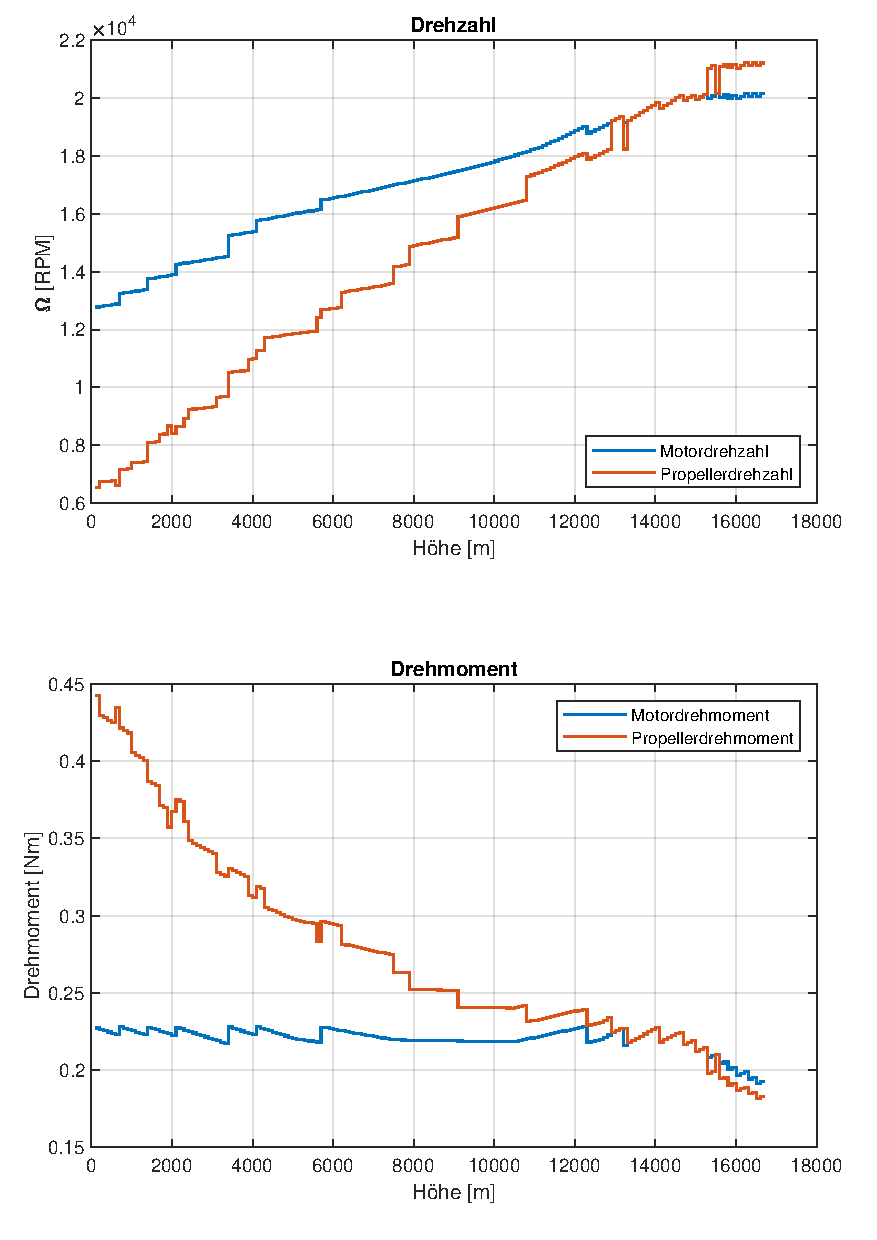
\includegraphics[scale=0.5]{Diagramme/Drehzahl_und_Drehmoment.pdf}
	\caption{Auswirkungen der Übersetzung des Getriebes auf die Drehzahl und das Drehmoment von Motor und Propeller}
	\label{abb:getriebe_dud}
\end{figure}

In der Realität besitzt ein stufenloses Getriebe oder CVT-Getriebe jedoch immer ein Eigengewicht und zeichnet sich durch einen vergleichsweise schlechten Wirkungsgrad aus \cite[S.295-S.297]{Fischer.2016}. %(\SI{0.8}{} zu etwa \SI{0.95}{} bei einem Stufengetriebe)
Die hohen Verluste können auf die hohe erforderliche Reibkraft und Verstellkraft zurückgeführt werden. Unter Berücksichtigung dieser verringert sich der Höhengewinn schrittweise, je größer das Getriebegewicht und dessen Verluste ausfallen. 
Zusätzlich ist anzuzweifeln, dass stufenlos verstellbare Getriebe im Modellbau existieren, die ein sehr geringes Eigengewicht besitzen und sich daher für Flugmodell eignen.
Das Gewicht eines einzelnen Getriebes beläuft sich dabei auf mehr als \SI{750}{g} \cite{cvt}, wobei die Verstellelektronik nicht berücksichtigt wurde. Für einen vierrotorigen Multicopter entspräche das einem Zusatzgewicht von mehr als \SI{3000}{g}. 
Die Vorteile eines CVT-Getriebes werden durch dessen Nachteile deutlich überkompensiert. Ein solches Getriebe bedeutet bei all seiner Kampaktheit und Effizienz letztendlich große Zusatzmasse und einen weiteren, verlustbehaftete Komponenten innerhalb der Antriebskette. Aus all diesen Gründen kann von dem Einsatz eines stufenlosen Getriebes für einen Multicopter abgesehen werden.


\section{Vorschlag einer optimalen Lösung}
\label{sec:otimale_lsg}
Aus den bisherigen Parameteruntersuchung soll nun eine optimale Konfiguration vorgestellt werden (vgl. Abschn. \ref{subsec:vorueberlegung}). Anschließend erfolgt die Darstellung der Flugleistungen unter idealen Randbedingungen (vgl. Abschn. \ref{subsec:ideale_rb}) und danach unter den Randbedingungen, die im AEROMET\_UAV-Projekt vorgegeben sind (vgl. Abschn. \ref{subsec:aeromot_rb}). 


\subsection{Vorüberlegungen}
\label{subsec:vorueberlegung}
Für den Antrieb ist ein Motor mit hohem \ensuremath{K_V}-Wert zu wählen, der zusätzlich wenige interne Verluste hat (vgl. Abschn. \ref{subsec:mot_prop_kombi}). In Bezug auf den gewählten Motor ist der Propeller auszuwählen. Eine Minimierung der aerodynamischen Verluste trägt zu einer Effizienzsteigerung bei (vgl. Kap. \ref{subsec:widerstandseinfluss}). Einen großen Einfluss auf die Flugleistungen hat die Batterie. Kurz zusammengefasst sollte die Batteriemasse einen Anteil von 2/3 der Gesamtmasse einnehmen (vgl. Kap. \ref{subsec:massenverteilung}). Dabei ist die Batteriezellenanzahl in Bezug auf den Motor festzulegen (vgl. Kap. \ref{subsec:einfluss_n_bat}).
Die optimale Anzahl der Propeller liegt zwischen vier und acht Propellern (vgl. Kap. \ref{subsec:anz_prop}). Es gibt kaum Unterschiede in den Flugleistungen dieser Konfigurationen. Ein Verstellpropeller bringt gewisse Vorteile mit, die die Dienstgipfelhöhe und den anschließenden Sinkflug betreffen. Allerdings werden diese durch die zusätzlichen Verluste überkompensiert (vgl. Kap. \ref{subsec:verstellprop}). Dies betrifft ebenso den hypothetischen Einsatz eines stufenlos verstellbaren Getriebes (vgl. Kap. \ref{subsec:getriebe}). \\
Die optimale Konfiguration ist in Tab. \ref{tab:optimale_konfiguration} konkretisiert.

\begin{center}
	\captionof{table}{wichtige Parameter der optimalen Multicopter-Konfiguration}
	\begin{tabular}{l l l} \hline
		Parameter & Variablenname & verwendete Größe \\ \hline
		Gesamtmasse \ensuremath{m} & \texttt{m} & \SI{3,504}{kg} \\
		Leermasse des Multicopters \ensuremath{m_{copter}}& \texttt{m\_copter} & \SI{1.028}{kg} \\ 
		Batteriemasse \ensuremath{m_{Bat}} & \texttt{m\_Bat} & \SI{2,052}{kg} \\
		Motormasse \ensuremath{m_{Mot}}& \texttt{m\_Mot} & \SI{106}{g} \\
		Geschwindigkeitskonstante \ensuremath{K_V} & \texttt{K\_V} & \SI{1390}{RPM/V} \\
		maximaler Dauerstrom \ensuremath{I_{max}} & \texttt{I\_max} & \SI{35}{A} \\
		Propeller & \texttt{prop\_name} & 11x4 \\
		Anzahl Propeller \ensuremath{n_{Prop}} & \texttt{n\_prop} & \SI{4}{} \\ 
		Anzahl der Batteriezellen \ensuremath{N_{Bat,cell}} & \texttt{N\_bat\_cell} & 5 \\	 
		Obere Stirnfläche \ensuremath{F_{copter,oben}} & \texttt{F\-copter\_oben} & \SI{0,0209}{m^2} \\
		Oberer Widerstandsbeiwert \ensuremath{c_{W,copter,oben}} & \texttt{c\_W\_copter\_oben} & 0,5 \\ \hline
	\end{tabular}	
	\label{tab:optimale_konfiguration}
\end{center}
Änderungen im Vergleich zu der Multicopter-Referenzkonfiguration (vgl. Tab. \ref{tab:referenzkonfiguration_mulitcopter}) ergeben sich unter anderem in der Batterie. Die Batteriezellenanzahl ist um eine Zelle verringert und die Batteriemasse auf einen Anteil von 2/3 an der Gesamtmasse erhöht worden. Weiterhin wird dem Quadrocopter eine aerodynamische günstige Form zugesprochen, weshalb der oberer Widerstandsbeiwert sich auf \SI{0,5}{} reduziert. Im Sinne einer Effizienzsteigerung wird auch die Propellersteigung um \SI{1}{in} erhöht, sodass der Propeller für die optimale Konfiguration ein 11x4 Propeller ist. Die letzte vorgenommene Änderung betrifft den Wirkungsgrad der Motorregler. An dieser Stelle wird davon ausgegangen, dass sich die Verluste innerhalb des Reglers halbieren. Die Leermasse, die obere Stirnfläche und die Motoren ändern sich nicht.


\subsection{Ideale Randbedingungen}
\label{subsec:ideale_rb}
Für die Untersuchung unter idealen Randbedingungen ist die Windgeschwindigkeit auf \SI{10}{m/s} gesetzt (vgl. Kap. \ref{sec:multicopter_referenzkonfig}) und es wird zusätzlich keine  Nutzlast mitgeführt.
Die bestmögliche Konfiguration erreicht eine Höhe von  mehr als \SI{18000}{m} (vgl. Abb. \ref{abb:optimale_konfig}). Auch dieses Mal erreicht die Konfiguration ihre Dienstgipfelhöhe, welche sich durch ein Absinken der Bahngeschwindigkeit ab \SI{12100}{m} gegen \SI{0}{m/s} auszeichnet. Der Grund für die Bahngeschwindigkeitsabnahme ist die limitierte Antriebsleistung. Sie ist am Ende der ausschlaggebende Parameter. Deutlich zu erkennen ist, dass die Motoren bereits zu Beginn des Fluges mit maximalem Motorstrom betrieben werden. Hier lassen sich zwei Gründe ausmachen.
Der Erste betrifft den Propeller. Der Propeller zeigt mit seinen \SI{11}{in} Durchmesser eine hohe Effizienz wie der TOC, die Restladung und der Propellerwirkungsgrad verdeutlichen. Jedoch bedeutet ein großer Propellerdurchmesser auch gleichzeitig ein hohes Propellerdrehmoment, was im Umkehrschluss einen hohen Motorstrom folgert (vgl. Gleichung \eqref{eq:motorstrom}). Deshalb wird der Propellerschub durch den maximalen Motorstrom von \SI{35}{A} limitiert. Rückwirkend wirkt sich dies auf die Bahngeschwindigkeit aus, die damit nach oben begrenzt ist. \\
Der zweite Grund umfasst das Gesamtgewicht. Die insgesamt \SI{3,504}{kg} Gesamtmasse stellen ein hohes Gewicht dar und gleichzeitig eine hohe Schubanforderung (vgl. Gleichung \eqref{eq:schub_multicopter}). Ähnlich zum Propeller erzeugt der hohe, benötigte Schub wieder einen großen Motorstrom. \\
Beide Gründe verursachen einen hohen Motorstrom, der eine Abriegelung der Motorleistung auf \ensuremath{I_{max}} erforderlich machen. Dem schließt sich eine Begrenzung der Bahngeschwindigkeit an. \\
Deutlich zu erkennen ist, dass der Motor jedoch nicht bei \SI{100}{\%} PWM betrieben wird. In diesem Sinne ist noch ein Leistungsüberschuss gegeben.
Die Batterie weist auf der Höhe von \SI{15000}{m} noch mehr als \SI{40}{\%} Restladung auf (vgl. Abb. \ref{abb:optimale_konfig}). Mit dieser Restladung ist somit im Anschluss an den Steigflug noch ein sicherer Sinkflug möglich. Das Fluggerät kann wieder unbeschadet landen.

\begin{figure}[H]
\centering
	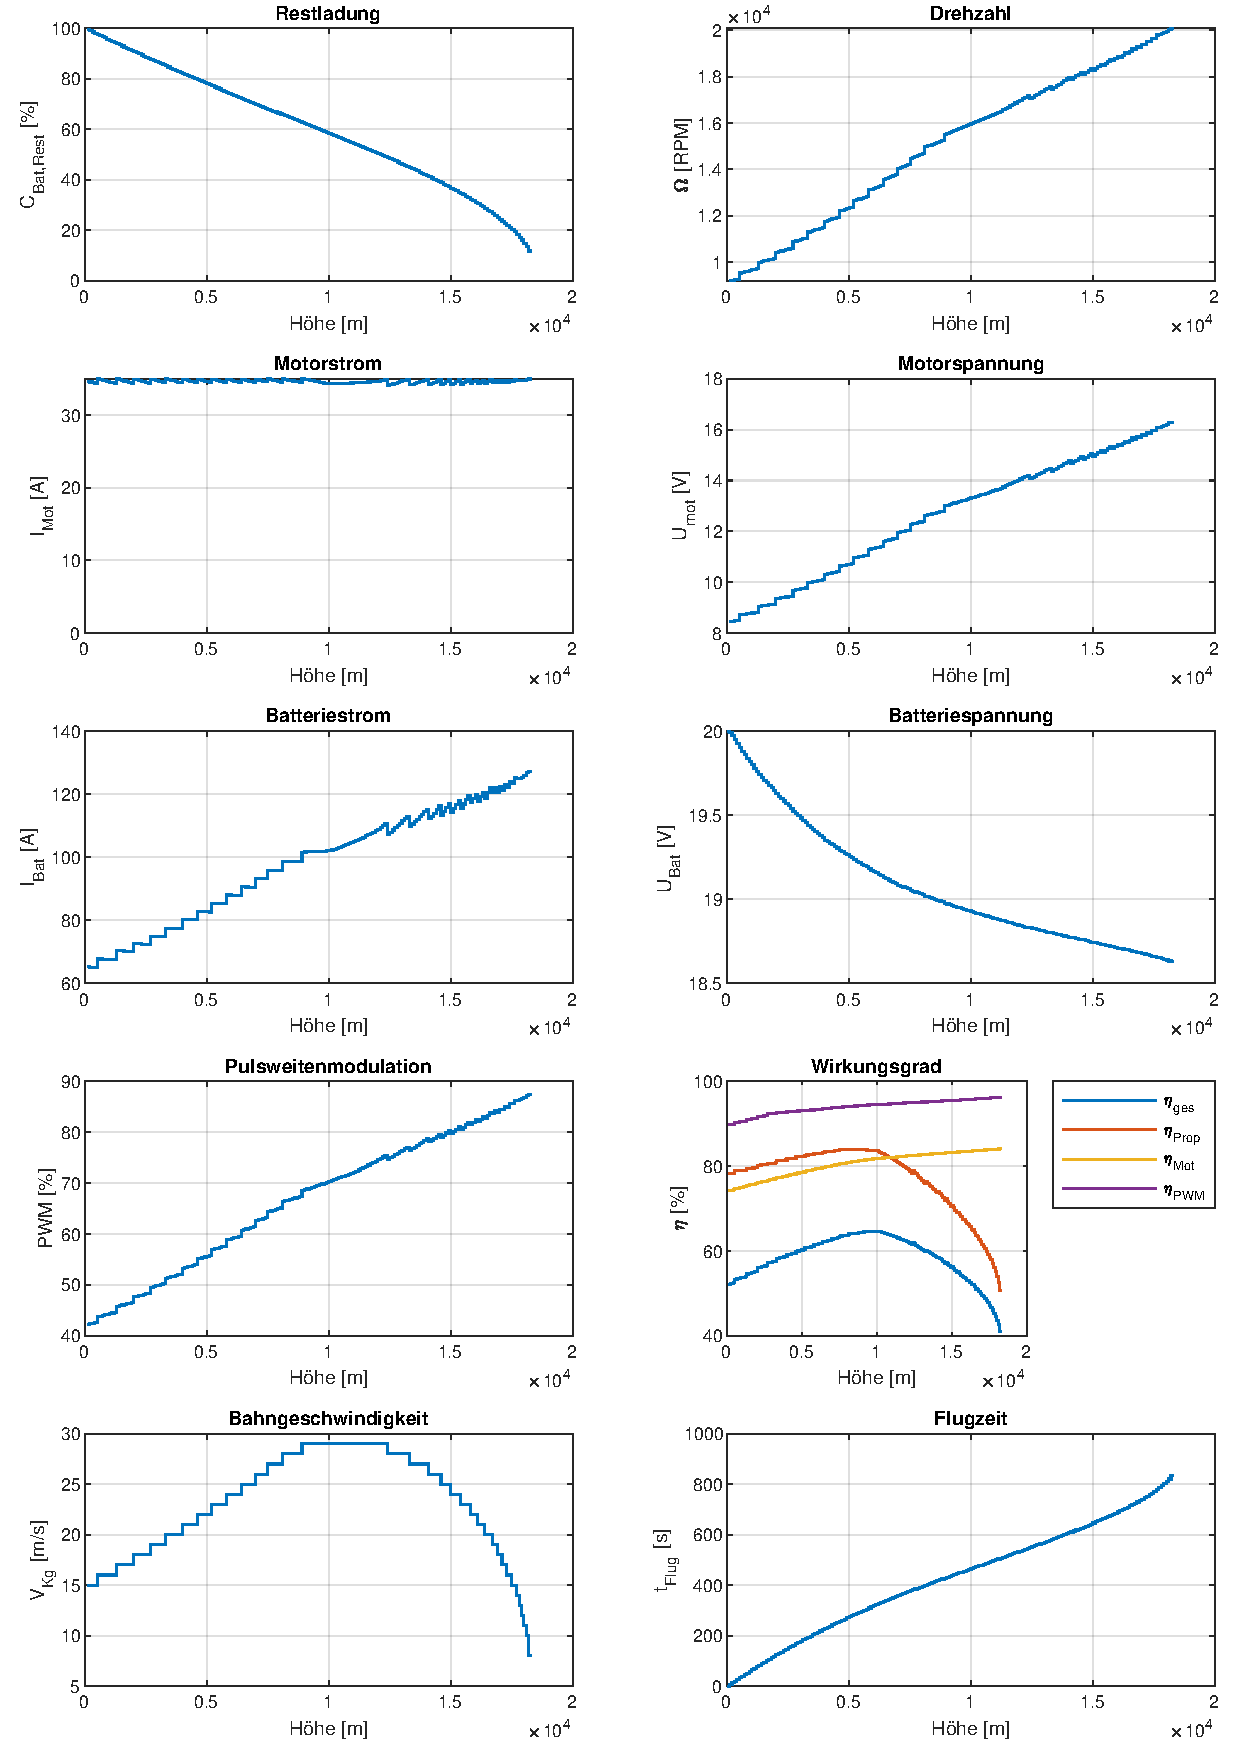
\includegraphics[scale=0.7]{Diagramme/Endergebnis.pdf}
	\caption{Die Flugleistungen der bestmöglichen Konfiguration (Tab. \ref{tab:optimale_konfiguration})}
	\label{abb:optimale_konfig}
\end{figure}



\subsection{AEROMET\_UAV Randbedingungen}
\label{subsec:aeromot_rb}
Schlussendlich soll noch der Einfluss der für dieses Projekt definierten Randbedingungen festgehalten werden. Die für das Projekt vorgeschriebenen Randbedingungen sind in Tab. \ref{tab:randbedingungen} aufgelistet. 
 
\begin{center}
\captionof{table}{wichtige Parameter des Flächenflugzeugs}
\begin{tabular}{l l l} \hline
	Parameter & Variablenname & verwendete Größe \\ \hline
	Windgeschwindigkeit \ensuremath{u_{Wg}} & \texttt{u\_Wg} & \SI{100}{km/h}\\
	Nutzlast \ensuremath{m_{Nutz}} & \texttt{m\_Nutz} & \SI{250}{g}  \\ \hline
\end{tabular}	
\label{tab:randbedingungen}
\end{center}

Erste Untersuchungen mit der optimalen Lösung aus Abschn. \ref{subsec:ideale_rb} haben ergeben, dass unter den AEROMET\_UAV-Randbedingungen maximal eine Höhe von \SI{8000}{m} erreicht werden kann. Hierbei wurde die Nutzlast auf die Gesamtmasse addiert. \\
Es existiert eine deutliche Korrelation zu den Aussagen in Abschn. \ref{subsec:ideale_rb}.\\
Durch das Zusatzgewicht der Nutzlast erhöht sich die Gesamtmasse zusätzlich. Damit steigt wiederum die Schubanforderung und letztlich der Motorstrom für jeden Höhenschritt. Dadurch erfolgt eine Abriegelung der Antriebsleistung schon bei geringen Bahngeschwindigkeiten und übrigen Leistungsparametergrößen. \\
Mit Bezug auf Abschn. \ref{subsec:propeller} und \ref{subsec:ideale_rb} ist eine Anpassung des Propellers vorzunehmen. Trotz der höheren Effizienz von größeren Propellerdurchmessern ist eine Verringerung dieses Parameters im Sinne einer Senkung des Propellerdrehmoments erforderlich. \\
Aus diesen Gründen sind kleine Änderungen an der optimalen Konfiguration vorzunehmen. Der Propellerdurchmesser wird um einen Inch verkleinert, sodass anstatt eines 11x4 ein 10x4 Propeller zum Einsatz kommt. Eine Reduzierung der Batteriemasse durch die Nutzlast erfolgt vorerst nicht. Der Zusammenhang wird im Folgenden und im Anhang \ref{sec:einfluss_nutzlast} genauer dargelegt.

\begin{figure}[H]
\centering
	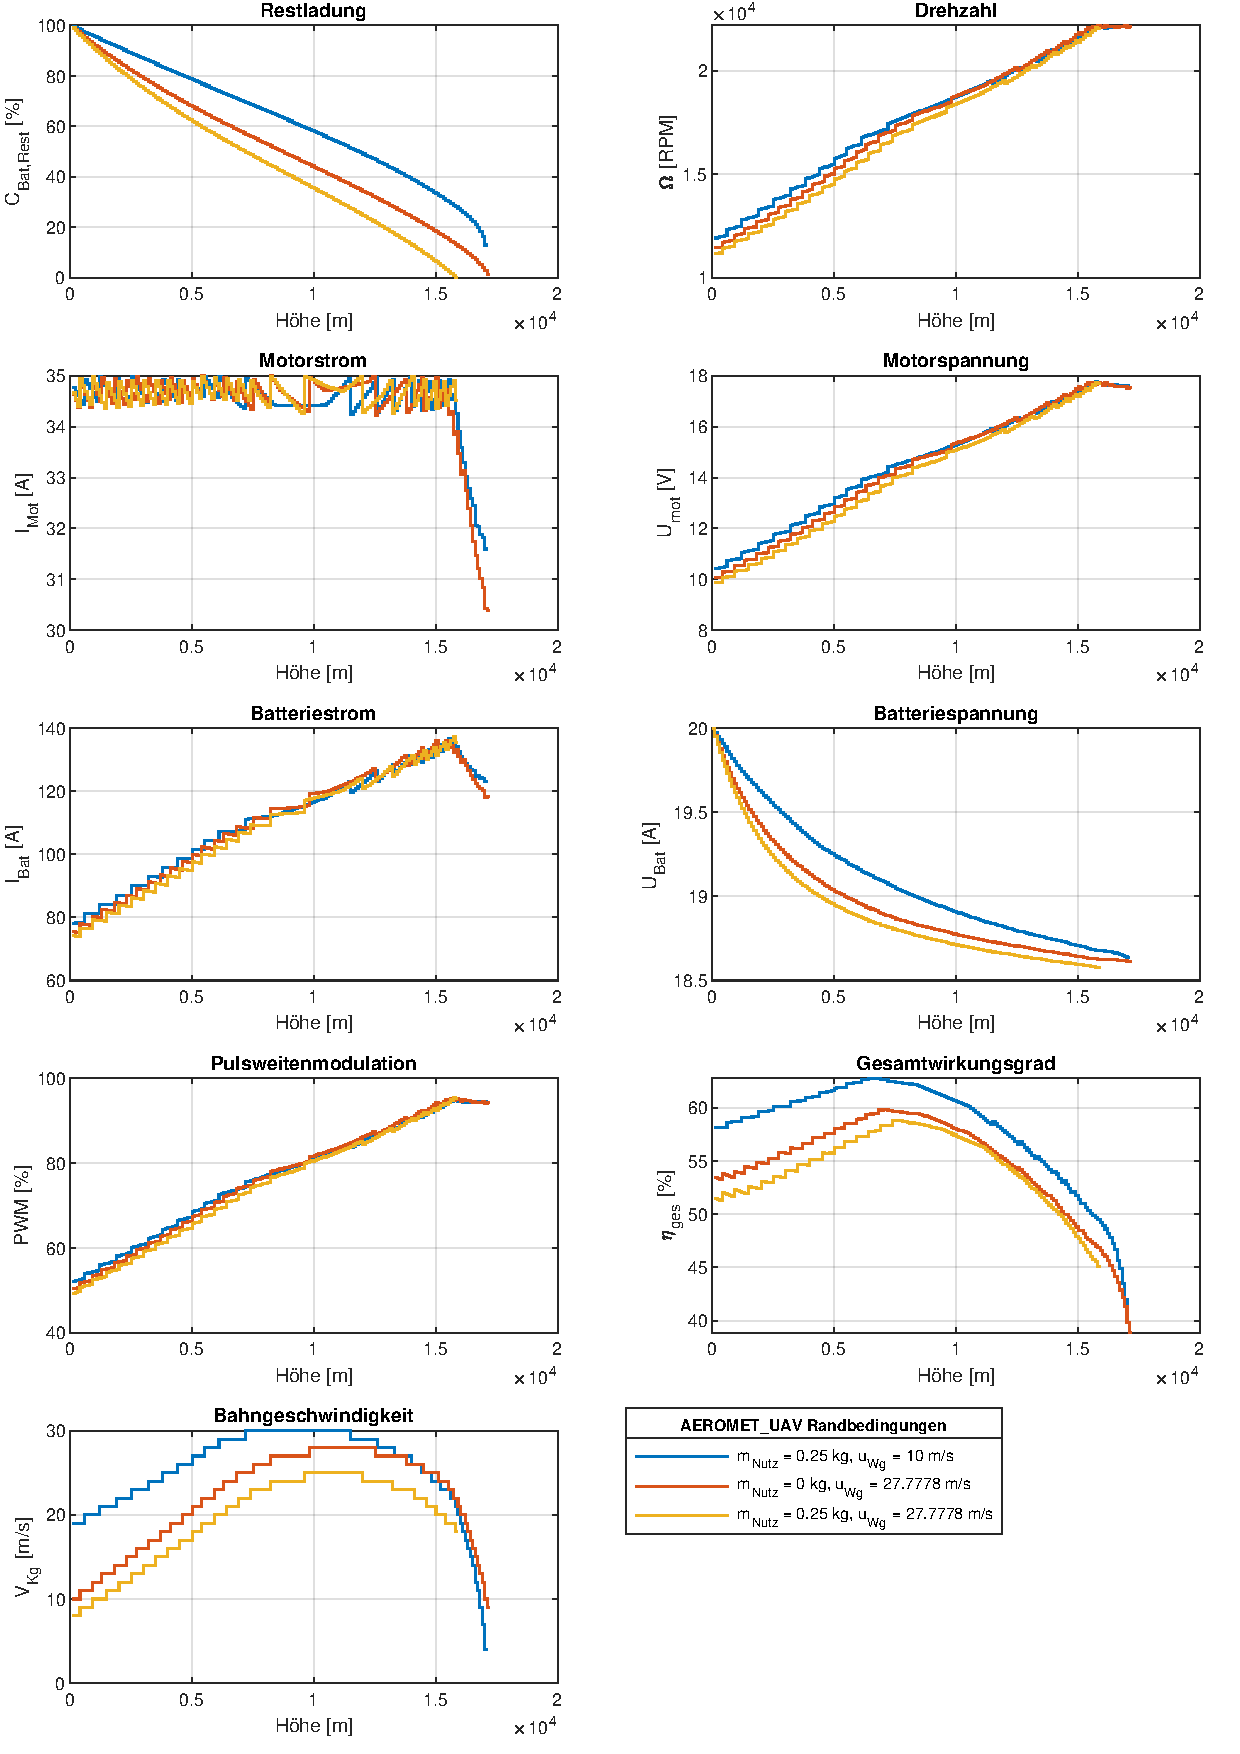
\includegraphics[scale=0.7]{Diagramme/aeromet_randbedingungen.pdf}
	\caption{Einfluss der AEROMET\_UAV-Randbedingungen auf die bestmögliche Konfiguration (Tab. \ref{tab:optimale_konfiguration})}
	\label{abb:aeromet_rb}
\end{figure}

Die Konfigurationen, die jeweils nur eine der Randbedingungen berücksichtigen, steigen beide bis zu ihrer Dienstgipfelhöhe auf. Diese liegt auf ca. \SI{18000}{m} Höhe (vgl. Abb. \ref{abb:aeromet_rb}). Der limitierende Parameter ist erneut die Propellerdrehzahl, die ab \SI{16000}{m} Höhe in den Bereich von einer Blattspitzengeschwindigkeit bei \ensuremath{Ma_{tip} = 1} kommt. Die Dienstgipfelhöhe verdeutlicht erneut die Notwendigkeit einer optimalen Propellerauswahl (vgl. Abschn. \ref{subsec:propeller} und \ref{subsec:vorueberlegung}). \\
Der Einfluss von \ensuremath{m_{Nutz}} ist im Vergleich zu der optimalen Konfiguration (vgl. Abschn. \ref{abb:optimale_konfig}) gering. Trotz der Verwendung eines kleineren Propellers beträgt die Differenz der Restladung z.B. auf \SI{15000}{m} Höhe gerade einmal \SI{4}{\%}. Anders ist der Einfluss der Seitenwindgeschwindigkeit. Diese verursacht einen starken Einbruch der Restladung bereits zu Beginn des Steigfluges (vgl. Abb. \ref{abb:aeromet_rb}). Im Laufe des Fluges ist die Batterierestladung im Durchschnitt ca. \SI{20}{\%} unterhalb des Restladungsverlauf der optimalen Konfiguration (vgl. Abb. \ref{abb:optimale_konfig}). Die Tendenz der Diskrepanzvergrößerung ist steigend.\\
Der Einfluss des Seitenwindes ist also bedeutend größer als der der Nutzlast. Je stärker der Seitenwind ist, desto größer ist der Energieaufwand zur Kompensation der Abdrift durch eine Neigung der Rotorebene. Diese Energie steht nun nicht mehr für einen Steigflug zur Verfügung. Folglich sinkt die Bahngeschwindigkeit und damit auch der Propellerwirkungsgrad \ensuremath{\eta_{prop}}. Dasselbe gilt für den Gesamtwirkungsgrad \ensuremath{\eta_{ges}}. \\
Das wirken beider Randbedingungen aus Tab. \ref{tab:randbedingungen} kommt einer Superposition des Nutzlasteinflusses und des Seitenwindeinflusses gleich. Die maximal erreichbare Flughöhe wird nochmals reduziert. Letztendlich können Flughöhen von \SI{15200}{m} erreicht werden. Die Restladung der Batterie verzeichnet eine schnellere Abnahme und der Gesamtwirkungsgrad ist am geringsten, was ebenso für die Bahngeschwindigkeit gilt. 

\subsection{Zusammenfassung}
\label{subsec:ergebnisse}
Die optimale Lösung aus aus Abschn. \ref{subsec:vorueberlegung} zeigt gute Flugleistungen, die noch eine ausreichende Restladung auf Dienstgipfelhöhe und somit einen anschließenden, sicheren Sinkflug gewährleistet. \\
Die Motoren werden durch den großen Propellerdurchmesser unter Idealbedingungen am oberen Leistungslimit durch den maximalen Motorstrom betrieben (vgl. Abschn. \ref{subsec:ideale_rb}). Dieser Zustand ist jedoch nachteilig für das Mitführen einer zusätzlichen Nutzlast und bei einem Flug mit höheren Seitenwinden. Eine Reduzierung des Propellerdurchmessers schafft Abhilfe. Weiterhin ist der Einfluss von starken Seitenwinden bedeutend größer als der der Nutzlast. Ein Verschlechterung der Flugleistungen durch deren kleiner Massenanteil an der Gesamtmasse ist begrenzt.\\
Ist der Quadrocopter zusätzlich mit aerodynamischen Vorrichtungen versehen, kann ein Gleitflug nach dem Erreichen des TOC eingeleitet werden, der nur noch einen wenig Energie beansprucht. Der Punkt vor dem zwingenden Einleiten des Sinkflugs verschiebt sich damit in noch größere Flughöhen.

    %\chapter{Parameteruntersuchung}
\label{chap:parameteruntersuchung}

\section{Einleitung und Vorgehensweise}
\label{sec:einleitung_und_vorgehensweise}
Grundlegend kann die Parameteruntersuchung wie eine Art Entscheidungsbaum aufgefasst werden. Dabei führt jede Entscheidung im Baum zu einer neuen Untersuchung und zu neuen Erkenntnissen. Im Verlaufe dieser Untersuchung werden somit Konzepte, Flugzustände, Komponenten und Konstellationen ausgewählt und intensiver betrachtet. Den Beginn zeichnet die grundlegende Frage aus, welches Fluggerätekonzept, i.e. Flächenflugzeug oder Multicopter, sich für einen effizienten Aufstieg in die untere Stratosphäre als optimaler erweist. \\
In der folgenden Parameteruntersuchung sei nochmal auf den Aufbau der Leistungsberechnung verwiesen, der dem eines realen Systems in umgekehrter Weise gegenübersteht (Kap. \ref{sec:leistungsberechnung}).

\section{Multicopter im Vergleich zu einem Flächenflugzeug}
\label{sec:multicopter_vs_flaechenflugzeug}
Jedes Luftfahrzeugkonzept entzieht sich einem direkten Vergleich mit einem Luftfahrzeug einer anderen Art. So weist jedes Fluggerät in seiner Gattung spezifische Vorteile auf wie der Start auf der Stelle und das Hovern in der Luft für Multicopter oder der Gleitflug für Flächenflugzeuge. Die optimale Auslegung beider führt zu unterschiedlichen Designs was die Propeller, die Motorleistung und -gewicht, Größe, Gesamtgewicht etc. betrifft. Aus diesem Grund müssen Kriterien für eine Vergleichbarkeit vorgeschrieben werden. Hierfür wird das Design des Multicopters auf das aus \cite{Anderson.2018} festgelegt, welches genauer in Kapitel \ref{sec:komponenten} beschrieben ist. Da die Flugleistungen von \cite{Anderson.2018} bekannt sind und der Quadrocopter durchaus schon im Rahmen der Anforderungen für diese Mission als optimiert betrachtet werden kann, bedarf es lediglich einer Untersuchung des Flächenflugzeuges. Dazu wird das Flächenflugzeug auf Parameter fixiert, mit denen es bereits sehr hoch aufsteigen kann. Zur Untersuchung und Vergleichbarkeit werden beide Gesamtmassen gleichgesetzt \ensuremath{m_{ges,Quadrocopter} = m_{ges,Flächenflugzeug}}. Dabei setzt sich die Masse der Flächenflugzeugbatterie   
\begin{equation}
	m_{Bat,Fl} = m_{Bat,Quad} + (m_{Mot,Quad}\cdot n_{Prop,Quad} - m_{Mot,Fl}\cdot n_{Prop,Fl}) - (1-f_P)\cdot m_{Quad}  
\end{equation}
in Bezug auf bereits gewählte Massen und auf den Quadrocopter zusammen. Der Faktor \ensuremath{f_P} kann als Penaltyfaktor verstanden werden. Dieser verringert zusätzlich die Batteriemasse, wenn das Strukturgewicht des Flächenflugzeugs das des Quadrocopters überschreitet
\begin{equation}
	f_P = \frac{m_{Flächenflugzeug}}{m_{Quad}}.
\end{equation} 
Für erste Untersuchungen wird der Penaltyfaktor auf 1 gesetzt. Dies entspricht einer sehr optimistischen Einschätzung. Im Anschluss werden die Parameter in näherer Umgebung der ersten festgesetzten Werte variiert. Dadurch kann der Einfluss auf das Leistungsverhalten und die Richtung der Optimierung bestimmt werden. Diese erste, einfache Untersuchung ist nur eine sehr oberflächliche, weil jeder Parameter nur einzeln untersucht wird. Jegliche Kombinationen von Einflüssen wie der Einfluss des Masse auf die Steiggeschwindigkeit oder vergleichbare Beziehungen werden vernachlässigt. Im Hinblick auf diese erste, kleine Optimierung ist der Kostenfaktor die maximal erreichbare Höhe beider Fluggeräte. Je nachdem welches der beiden Fluggeräte effektiver und effizienter eine maximale Flughöhe erreicht, wird es weiter untersucht und anschließend optimiert. 


\subsection{Erste Untersuchung}
\label{subsec:erste_untersuchung}
In der folgenden Tabelle sind wichtige Parameter der Ausgangskonstellation für das Flächenflugzeuges aufgelistet.
\todo[inline]{check die Einheit vom KV Wert}
\begin{center}
	\captionof{table}{wichtige Parameter des Flächenflugzeugs}
	\begin{tabular}{l l l} \hline
		Parameter & Variablenname & Wert \\ \hline
		Motormasse \ensuremath{m_{Mot}}& \texttt{m\_Mot} & \SI{106}{g} \\
		Geschwindigkeitskonstante \ensuremath{K_V} & \texttt{K\_V} & \SI{1390}{RPM/V} \\
		maximaler Dauerstrom \ensuremath{I_{max}} & \texttt{I\_max} & \SI{25}{A} \\
		Propeller & \texttt{prop\_name} & 9x7 \\
		Anzahl Propeller \ensuremath{n_{Prop}} & \texttt{n\_prop} & \SI{1}{} \\
		Auslegungsgleitzahl \ensuremath{E^{\star}} & \texttt{E\_stern} & \SI{4}{} \\
		Auslegungsgeschwindigkeit \ensuremath{V^{\star}} & \texttt{V\_stern} & \SI{100}{km/h} \\
		Gleitzahl \ensuremath{E} & \texttt{E} & \SI{4}{} \\ \hline
	\end{tabular}	
	\label{tab:flzg_parameter}
\end{center}

\begin{figure}[H]
%\centering
	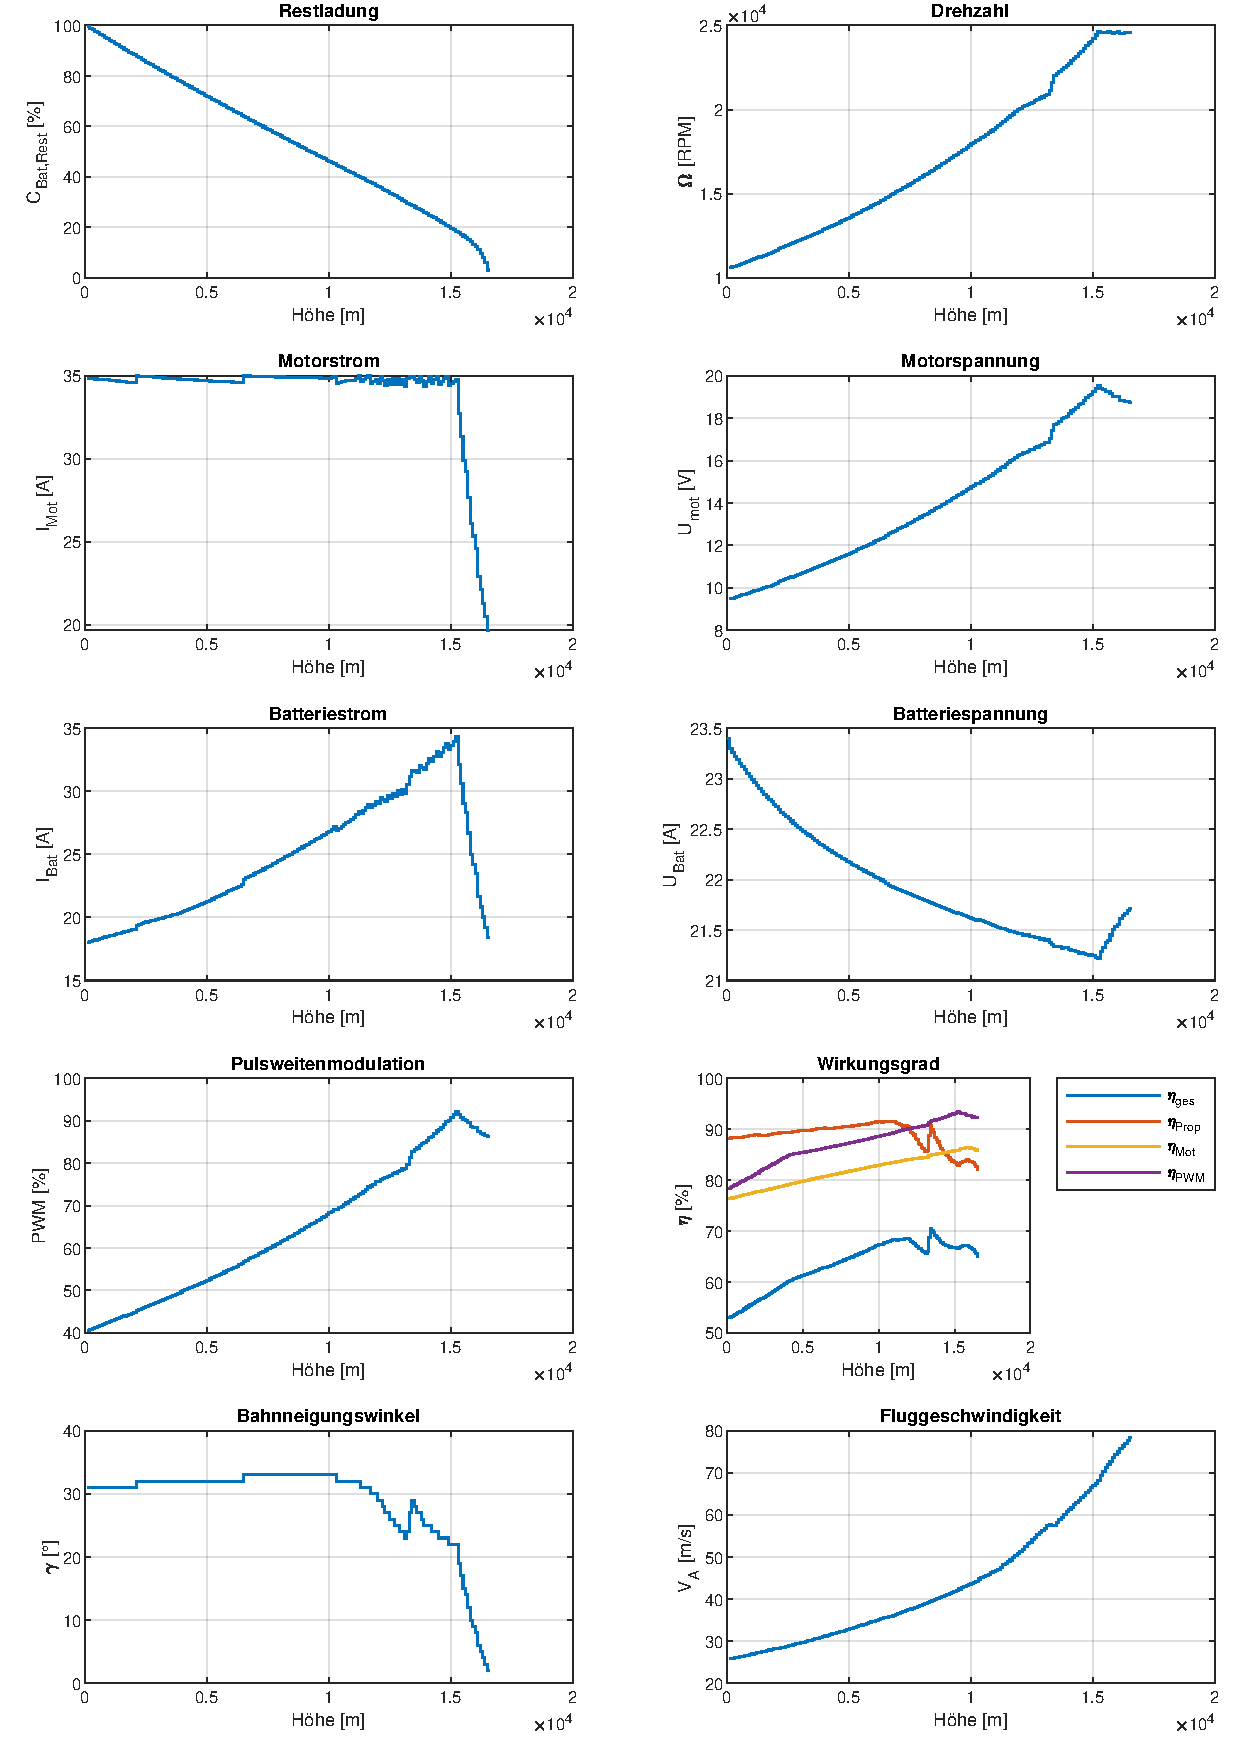
\includegraphics[scale=0.7]{Diagramme/Ausgangskonstellation.pdf}
	\caption{Verlauf der Leistungsparameter über der Höhe für ein Flächenflugzeug mit den in Tabelle \ref{tab:flzg_parameter} definierten Parametern}
	\label{abb:ausgangskonstellation}
\end{figure}

Die gewählte Konstellation erreicht mehr als \SI{13000}{m} Höhe (Vgl. Abb. \ref{abb:ausgangskonstellation}). Der die Höhe begrenzende Faktor ist in diesem Fall die fehlende Leistung zum Aufstieg in noch größere Höhen. Zu Beginn des Steigflugs stellt sich ein optimaler Bahnneigungswinkel von ca. \SI{31}{^\circ} bis \SI{33}{^\star} ein. Dieser Winkel kann bis zu einer Höhe \SI{9800}{m} gehalten werden. Dabei steigt die absolute Fluggeschwindigkeit leicht quadratisch mit dem Produkt aus \ensuremath{\sqrt{\rho^\star/\rho}} an (Vgl. Gleichung \ref{eq:geschw_flaechenflugzeug}). Zu Beginn des Steigfluges wären größere Steigwinkel effizienter, allerdings werden diese durch den maximalen Motorstrom (\ensuremath{I_{max} = \SI{35}{A}}) begrenzt. Ohne diesen würde der Bahnneigungswinkel beinahe linear absinken. Daraus kann geschlossen werden, dass ein Flug mit maximalem Motorstrom im unteren Höhenbereich am effizientesten ist. Der sägezahnartige Verlauf des Motorstroms hängt mit der gewählten Diskretisierung und dadurch rückwirkend mit der Genauigkeit zusammen. Eine genauere Untersuchung dieser Punkte würde zu einem glatten Verlauf des Motorstroms bei \ensuremath{I_{max}} führen. Ebenso würden sich die Verläufe aller anderen Leistungsparameter über der Höhe glätten. Gleichzeitig zum konstanten Motorstrom wächst die Motorspannung linear an, bis diese ab \SI{98000}{m} das Niveau der Batteriespannung erreicht. Damit ist das Verhältnis von \ensuremath{U_{Mot}} und \ensuremath{U_{Bat}} gleich 1 und  die PWM liegt bei \SI{100}{\%}. Ab diesem Zeitpunkt kann die Leistung für die Geschwindigkeit und den Schub bei einem konstanten Steigwinkel nicht mehr aufgebracht werden. Der Zusammenhang ergibt sich daher, dass mit dem Bahnanstellwinkel und der Höhe (indirekt durch die Dichte) der Schub und die Geschwindigkeit steigen (Vgl. Gleichung \ref{eq:schub_flaechenflugzeug} und \ref{eq:schub_flaechenflugzeug}). Außerdem wird der Motor bereits bei Vollast betrieben. Die maximale Motorspannung entspricht hier der maximalen Batteriespannung, die durch die Last von anfänglich \SI{15,5}{V} auf ca. \SI{14.45}{V} einbricht. Der Verlauf des Batteriestroms steht in direktem Zusammenhang mit dem Motorstrom und der Motorspannung. Dies wird aus Gleichung \ref{eq:batteriestrom} ersichtlich. Bei einem konstantem Motorstrom ist  \ensuremath{I_{Bat}} nur von \ensuremath{U_{Mot}} abhängig. Daher der gleiche Verlauf wie bei \ensuremath{U_{Mot}}. Danach ist \ensuremath{U_{Mot}} beinahe konstant und \ensuremath{I_{Bat}} hängt nur noch von \ensuremath{I_{Mot}} ab. Der Verlauf der Drehzahl ist ausschlaggebend für den des Motorspannung. Da die Motorspannung nicht weiter steigen kann und der Motorstrom leicht absinkt, kann die Drehzahl analog zum sinkenden Strom durch die festgelegten Grenzen leicht steigen (Vgl. Gleichung \ref{eq:motorspannung}). Die Maximaldrehzahl kann damit nur noch leicht auf \SI{19000}{RPM} steigen. 
Die Restladung nimmt mit der Höhe linear ab. Erst ab dem Flugzustand mit \SI{100}{\%} PWM nimmt die Restladung der Batterie deutlich schneller ab. Am höchsten Punkt des Aufstiegs können noch min. \SI{20}{\%} Restladung verzeichnet werden.
Der Gesamtwirkungsgrad gliedert sich wie in Kap. \ref{subsec:eta_ges} dargelegt in den Propeller-, den Motor- und den Motorreglerwirkungsgrad. Daher folgt er zeitgleich den anderen Wirkungsgraden. Der Propellerwirkungsgrad steigt mit der Höhe an. Ausschlaggebend hierfür ist die steigende Geschwindigkeit und die Drehzahl (Vgl. Gleichung \ref{eq:eta_prop}). Während der noch flugleistungstechnisch erreichbare Bahnneigungswinkel abfällt, steigt die Bahngeschwindigkeit und der Propellerwirkungsgrad. Über Gleichung \ref{eq:geschw_flaechenflugzeug} nimmt mit steigendem Bahnneigungswinkel die Fluggeschwindigkeit ab. Da dieser jedoch nun absinkt, nimmt damit auch die Fluggeschwindigkeit zu. Da die Motorspannung bereits ihr Maximum erreicht hat, kann die Propellerdrehzahl nur noch leicht mit der abnehmenden Dichte und somit geringer werdenden Widerstandskräften ansteigen (Vgl. Gleichung \ref{eq:motorspannung}. Dabei nimmt auch das Propellerdrehmoment ab (Ergebnis aus Gleichung \ref{eq:motorstrom}). Bei einer gleichermaßen steigenden absoluten Fluggeschwindigkeit, steigt die Strahlleistung des Propellers (Vgl. Gleichung \ref{eq:strahlleistung}). Als Konsequenz steigt der Propellerwirkungsgrad.
Dies gilt auch für den Motorwirkungsgrad. Dieser steigt mit einer anwachsenden Propellerdrehzahl und -drehmoment (Vgl. Gleichung \ref{eq:eta_mot}). Außerdem nehmen die durch den Innenwiderstand und den Leerlaufstrom verursachten Verluste anteilig am Motorstrom und der -spannung ab (Vgl. Gleichung \ref{eq:motorstrom} und \ref{motorspannung}), die mit zunehmender Höhe auch zunehmen. Der Grund hierfür liegt in der Annahme, dass diese beiden Motorkenngrößen für jeden Motorzustand als konstant angesehen werden. Der Wirkungsgrad des ESC steigt simultan mit der Höhe und der PWM. Mit steigender PWM nehmen auch die Verluste innerhalb des Motorreglers ab (Vgl. Gleichung \ref{eq:eta_pwm}). Deutlich zu erkennen ist eine Abnahme aller Wirkungsgrade, wenn die PWM \SI{100}{\%} erreicht und damit der Motorstrom sowie der Bahnneigungswinkel absinken. Dies ist ein Indiz für den Beginn eines ineffizienteren Flugzustandes.



% Die maximale Motorspannung entspricht ab \SI{11400}{m} Flughöhe der maximalen Batteriespannung, die durch die Last von anfänglich \SI{15,6}{V} auf ca. \SI{14.7}{V} einbricht. Der Verlauf des Batteriestroms steht in direktem Zusammenhang mit dem Motorstrom und der Motorspannung. Dies wird aus Gleichung \ref{eq:batteriestrom} ersichtlich. Bei einem beinahe konstantem Motorstrom ist \ensuremath{I_{Bat}} fast ausschließlich von \ensuremath{U_{Mot}} abhängig. Daher der gleiche Verlauf wie bei \ensuremath{U_{Mot}}. Danach ist \ensuremath{U_{Mot}} konstant und \ensuremath{I_{Bat}} hängt nur noch von \ensuremath{I_{Mot}} ab. 
%Der Verlauf der Drehzahl ist ausschlaggebend für den des Motorspannung. Da die Motorspannung nicht weiter steigen kann und der Motorstrom leicht absinkt, kann die Drehzahl analog zum sinkenden Strom durch die festgelegten Grenzen leicht steigen (Vgl. Gleichung \ref{eq:motorspannung}). Die Maximaldrehzahl ist damit auf \SI{12000}{RPM} begrenzt. 

%Zu Beginn des Steigfluges wären größere Steigwinkel effizienter, allerdings werden diese durch den maximalen Motorstrom begrenzt. Ohne diese würde der Bahnneigungswinkel beinahe linear absinken. Daraus kann geschlossen werden, dass ein Flug mit maximalem Motorstrom im unteren Höhenbereich am effizientesten ist. Der sägezahnartige Verlauf der Motorspannung hängt mit der gewählten Diskretisierung / Genauigkeit zusammen. Eine genauere Untersuchung dieser Punkte würde zu einem glatten Verlauf des Motorstroms bei \ensuremath{I_{max}} führen. Ebenso würde sich der Verlauf aller anderen Kurven glätten. Gleichzeitig zum konstanten Motorstrom wächst die Motorspannung linear an, bis sie ab \SI{11400}{m} das Niveau der Batteriespannung erreicht. Damit ist die PWM bei \SI{100}{\%}. Ab diesem Zeitpunkt kann nicht mehr mit maximalem Motorstrom geflogen werden, \textcolor{red}{wodurch folglich der Motorspannung und der Bahnneigungswinkel simultan abfallen}. 
%Der Zusammenhang ergibt sich daher, dass mit dem Bahnanstellwinkel der Schub und die Geschwindigkeit steigen (Vgl. Gleichung \ref{eq:schub_flaechenflugzeug} und \ref{eq:schub_flaechenflugzeug}). Die im Anschluss aus dem Kennfeld interpolierte Drehzahl fließt direkt in den Motorstrom ein (Vgl. Gleichung \ref{eq:motorstrom}). Bedingt durch die mit dem Winkel und der Höhe (indirekt durch die Dichte) steigende Geschwindigkeit, können die Steigwinkel leistungsbedingt nicht mehr aufgebracht werden. Die maximale Motorspannung entspricht hier der maximalen Batteriespannung, die durch die Last von anfänglich \SI{15,6}{V} auf ca. \SI{14.7}{V} einbricht. Der Verlauf des Batteriestroms steht in direktem Zusammenhang mit dem Motorstrom und der Motorspannung. Dies wird aus Gleichung \ref{eq:batteriestrom} ersichtlich. Bei konstanten Motorstrom ist die \ensuremath{I_{Bat}} nur von \ensuremath{U_{Mot}} abhängig. Daher der gleiche Verlauf wie bei \ensuremath{U_{Mot}}. Danach ist \ensuremath{U_{Mot}} konstant und \ensuremath{I_{Bat}} hängt nur noch von \ensuremath{I_{Mot}} ab.

%Gleichzeitig steigt der Motorstrom leicht, da für einen konstanten Bahnneigungswinkel der benötigte Schub konstant bleibt (Vgl. Gleichung \ref{eq:schub_flaechenflugzeug}), aber mit abnehmenden Dichte das Drehmoment zunimmt. Noch stärker als der Motorstrom steigt die Motorspannung linear an, bis sie das Niveau des Batteriestroms erreicht. Damit ist das Verhältnis von \ensuremath{U_{Mot}} und \ensuremath{U_{Bat}} gleich 1 und  die PWM liegt bei \SI{100}{\%}. Ab diesem Zeitpunkt kann \textcolor{red}{leistungsbedingt} die Geschwindigkeit und Schub für einen konstanten Steigwinkel nicht mehr gehalten werden. Folglich sinkt der Bahnneigungswinkel, da für ein Höhenintervall die absolute Fluggeschwindigkeit und analog die Steiggeschwindigkeit \ensuremath{V_H} mit einem mit einem  größeren Bahnneigungswinkel sinkt (Vgl. Gleichung \ref{eq:geschw_flaechenflugzeug}).


\subsection{Einflussfaktoren auf das Flächenflugzeug}
Die zu variierenden Parameter des Flächenflugzeugs sind diejenigen Leistungsparameter, die das Fluggerät qualifizieren. Das sind die Motor-Propeller-Kombination, die Propelleranzahl, die Gleitzahl, die Auslegungsgeschwindigkeit und der Penalty-Faktor.

\subsubsection{Motor-Propeller Kombination}
\label{subsubsec:mot_prop_kombi}
Die Motor-Propeller-Kombination beeinflusst entscheidend das Leistungsverhalten von elektrisch, propellergetriebenen Fluggeräten. Mit dem in Tab. \ref{tab:flzg_parameter} aufgeführten Motor mit einem Gewicht von \SI{106}{g} und einem \ensuremath{K_V}-Wert von \SI{1390}{RPM/V} sind bereits sehr hohe Flughöhen erreichbar. Bei Verwendung des gleichen Propellers, einem 9x7 Propeller, und der Variation des \ensuremath{K_V}-Wertes, zeigen die Motoren mit einem größeren \ensuremath{K_V}-Wert ein besseres Flugverhalten (Vgl. Abb. \ref{abb:flaechenflzg_mot_prop}).\\
Die optimale Flugweise des Flächenflugzeuges ist für jede Art des Motors mit gleichem Gewicht identisch. Zuerst wird solange mit maximalem Motorstrom geflogen, bis die Schubhebelstellung \SI{100}{\%} erreicht. Danach sinkt der Bahnneigungswinkel während die Steiggeschwindigkeit steigt. Die maximale Höhe ist erreicht, wenn der noch fliegbare Steigwinkel Null erreicht und kein Steigflug mehr möglich ist. Der Steigwinkel legt dabei in einem Bereich von \SI{15}{^\circ} und \SI{20}{^\circ}. \\
Mit dem \ensuremath{K_V}-Wert steigt ebenso die maximale Höhe (Vgl. Abb. \ref{abb:flaechenflzg_mot_prop}). Den größten Einfluss auf die Flugleistung hat der \ensuremath{K_V}-Wert auf die Motorspannung. Hier gilt, dass bei einer annähernd gleichen Drehzahl die Motorspannung mit dem \ensuremath{K_V}-Wert sinkt. Der Grund dafür liegt in der Definition dieses Motorkennwertes.\\

\begin{figure}[H]
\centering
	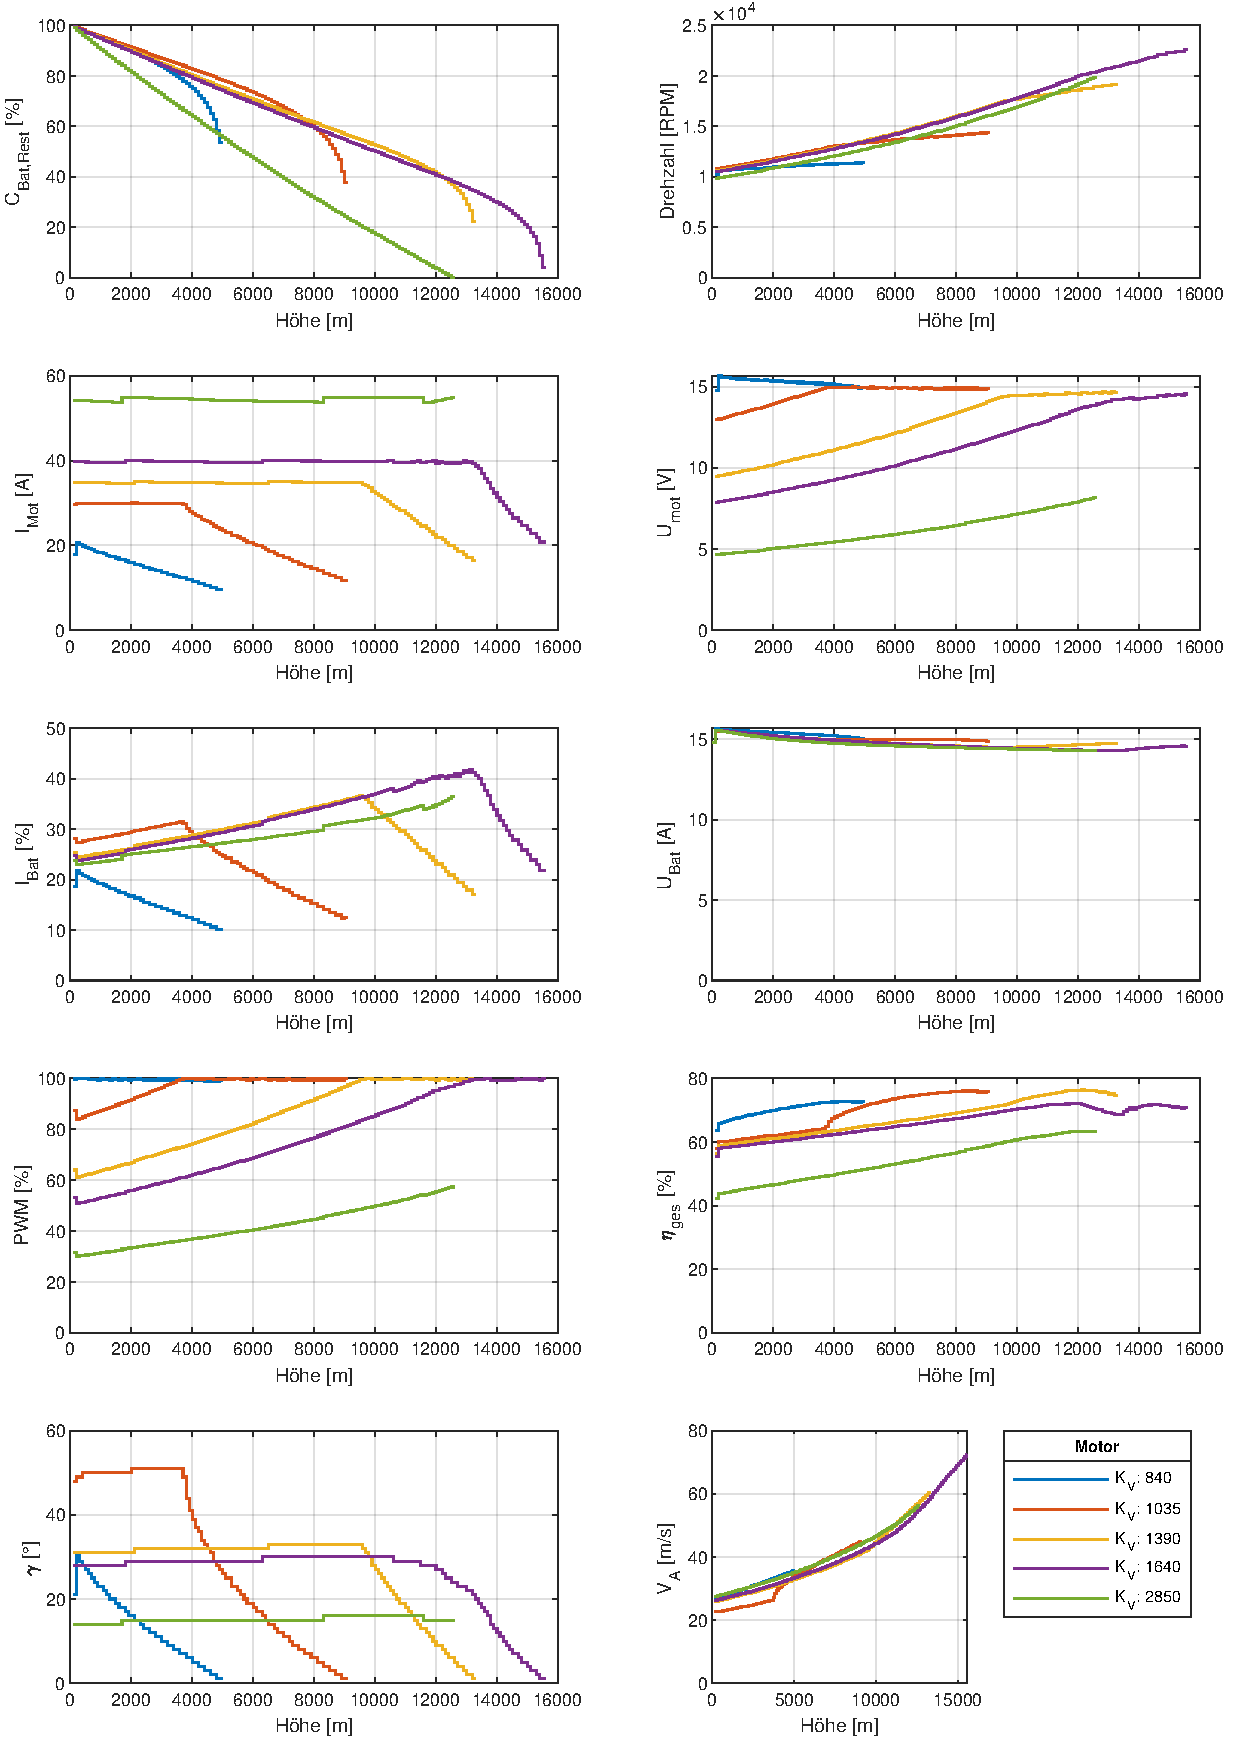
\includegraphics[scale=0.7]{Diagramme/Flaechenflzg_Mot_Prop.pdf}
	\caption{Einfluss der Motor-Propeller-Kombination auf die Flugleistungen eines Flächenflugzeugs (\ensuremath{m_{Mot}} = \SI{106}{g}, Propeller = 9x7)}
	\label{abb:flaechenflzg_mot_prop}
\end{figure}

Der \ensuremath{K_V}-Wert ist ein Kennwert für die Anzahl der Umdrehungen pro Minute pro Volt im Leerlauf. Ein hoher \ensuremath{K_V}-Wert bedeutet nun im Umkehrschluss, dass bei einer hohen Drehzahl die Spannung geringer ist als für einen Motor mit einem vergleichsweise niedrigem \ensuremath{K_V}-Wert. Gleichzeitig sinkt allerdings das Verhältnis von Drehmoment pro Ampere, das der \ensuremath{K_M}-ausdrückt  \cite[S.35 und S.42-43]{Buchi.2013}. Es gilt die Beziehung
\begin{equation}
	K_M = 1/K_V\cdot 30/\pi.
\end{equation}
Ein Motor mit hohem \ensuremath{K_V}-Wert muss daher einen hohen Dauermotorstrom besitzen, um gute Flugleistungen zu erzielen (Vgl. Abb. \ref{abb:flaechenflzg_mot_prop}). Dies ergeben auch die Ergebnisse in Abb. \ref{abb:flaechenflzg_mot_prop}. Durch diese Abhängigkeit wird auch die PWM beeinflusst. Der Motor mit einem \ensuremath{K_V} von \SI{840}{RPM/V} erreicht durch seine hohe Motorspannung deutlich schneller das Niveau der Batteriespannung. Somit wird auch frühzeitiger das Absinken des Bahnneigungswinkels eingeleitet, weil die maximale Motorleistung erreicht ist. Für Motoren mit einem niedrigeren \ensuremath{K_V}-Wert bedeutet dies auch gleichzeitig das Ende des Steigfluges. Wieder anders ist dieser Zusammenhang für Motoren mit einem hohen \ensuremath{K_V}-Wert. Hier wird \SI{100}{\%} PWM erst bei deutlich größeren Höhen erreicht, weshalb folglich der optimale Bahnneigungswinkel erst später nicht mehr gehalten werden kann und danach abflacht. Den Steigflug begrenzt in diesem Fall die Restladung. Dabei nimmt die Restladung für kleinere \ensuremath{K_V}-Werte nicht so schnell ab wie dies für große der Fall ist. Die kann auf den höheren Gesamtwirkungsgrad und im Detail auf den höheren \textcolor{red}{Motorreglerwirkungsgrad zurückgeführt werden auch ein höherer Motorwirkungsgrad bei höherer Spannung}. Durch die deutlich höhere Pulsweitenmodulation ist der Wirkungsgrad des Motorreglers entsprechend höher (Vgl. Gleichung \ref{eq:eta_pwm}. Außerdem sind die Verluste durch Temperatur  sowie Innenwiderstand oder Leerlaufstrom für einen Motoren mit niedrigem \ensuremath{K_V}-Wert geringer.\\
An dieser Stelle ist auch die Motor-Propeller Kombination zu beachten. Der Motor mit einem \ensuremath{K_V}-Wert von 2850 erzielt mit dem 9x7 Propeller zwar etwas schlechtere Flugleistungen, erreicht mit einem 6x4 Propeller jedoch noch größere Höhen (siehe Anhang). Zusammengenommen zeigt sich, dass mit geringer werdenden \ensuremath{K_V}-Wert, also einem langsamer, aber mit höherem Drehmoment drehender Motor, der optimale Durchmesser des Propellers in reziproker Weise steigt bei einem gleichen Verhältnis zwischen Durchmesser und Steigung. Dies kann relativ einfach mit den Angaben der Hersteller zu der besten Motor-Propeller-Kombination verglichen werden. Nach \cite{Wall.2015} erhöht sich der Wirkungsgrad eines Rotors mit größer werdenden Durchmesser. 
Mit den oben gemachten Aussagen zu einer Motor-Propeller-Kombination wird im Folgenden der Propeller an die Wahl der Motoren angepasst.
\textcolor{red}{hier anbringen, dass Effizienz von einem Motor mit geringem kV höher ist, weniger Verluste und weniger Erhitzung, 
http://rcboats.kiwi/index.php/ct-menu-item-15/ct-menu-item-31/ct-menu-item-43}


\subsubsection{Anzahl der Motoren und Propeller}
Während die Leistung der Motoren mit gleichem Gewicht wenig Einfluss auf den optimalen Steigwinkel hat, ändert sich dies bedeutend mit der Anzahl der Motoren. Schon mit einer Steigerung der Motorenanzahl auf 2 verändert sich der optimale Steigwinkel zu \SI{90}{^\circ}. Die dazu zugehörige Steiggeschwindigkeit liegt hierbei beim Maximum der Steiggeschwindigkeitsiterationsweite. Dies ist solange der optimale Betriebspunkt bis der Steigwinkel von \SI{55}{^\circ} optimaler ist.
Ebenfalls wie oben beschrieben ist dieser Zustand so lange fliegbar bis der Motorstrom auf dem Niveau des Batteriestroms und damit \SI{100}{\%} der PWM erreicht ist. Ab diesem Punkt steigt der Bahnneigungswinkel wieder an, da für einen Höhenschritt die Fluggeschwindigkeit mit Winkel sinkt. Alle anderen Größen verhalten sich analog zum oben beschriebenen Zustand (Vgl. Kap. \ref{subsec:erste_untersuchung}). Ein vergleichbares Flugverhalten ist bei einer Erhöhung der Anzahl auf 4 zu beobachten.
Mit der Propelleranzahl verringert sich der Schub, der pro Propeller aufgebracht werden muss und damit auch die vom Motor benötigte Leistung. Folglich erhöht sich auch der Leistungsüberschuss. Dies resultiert auf der anderen Seite in einer höheren Belastung der Batterie. Beachtlich ist auch, dass die Batterie am TOC noch beinahe \SI{50}{\%} Restladung besitzt. Dies ist signifikant mehr als beim Quadrocopter. Bei diesem ist der Steigflug beendet, wenn die Batterie leer ist. Beim Flächenflugzeug ist die Motorleistung der limitierende Parameter.

\begin{figure}[H]
\centering
	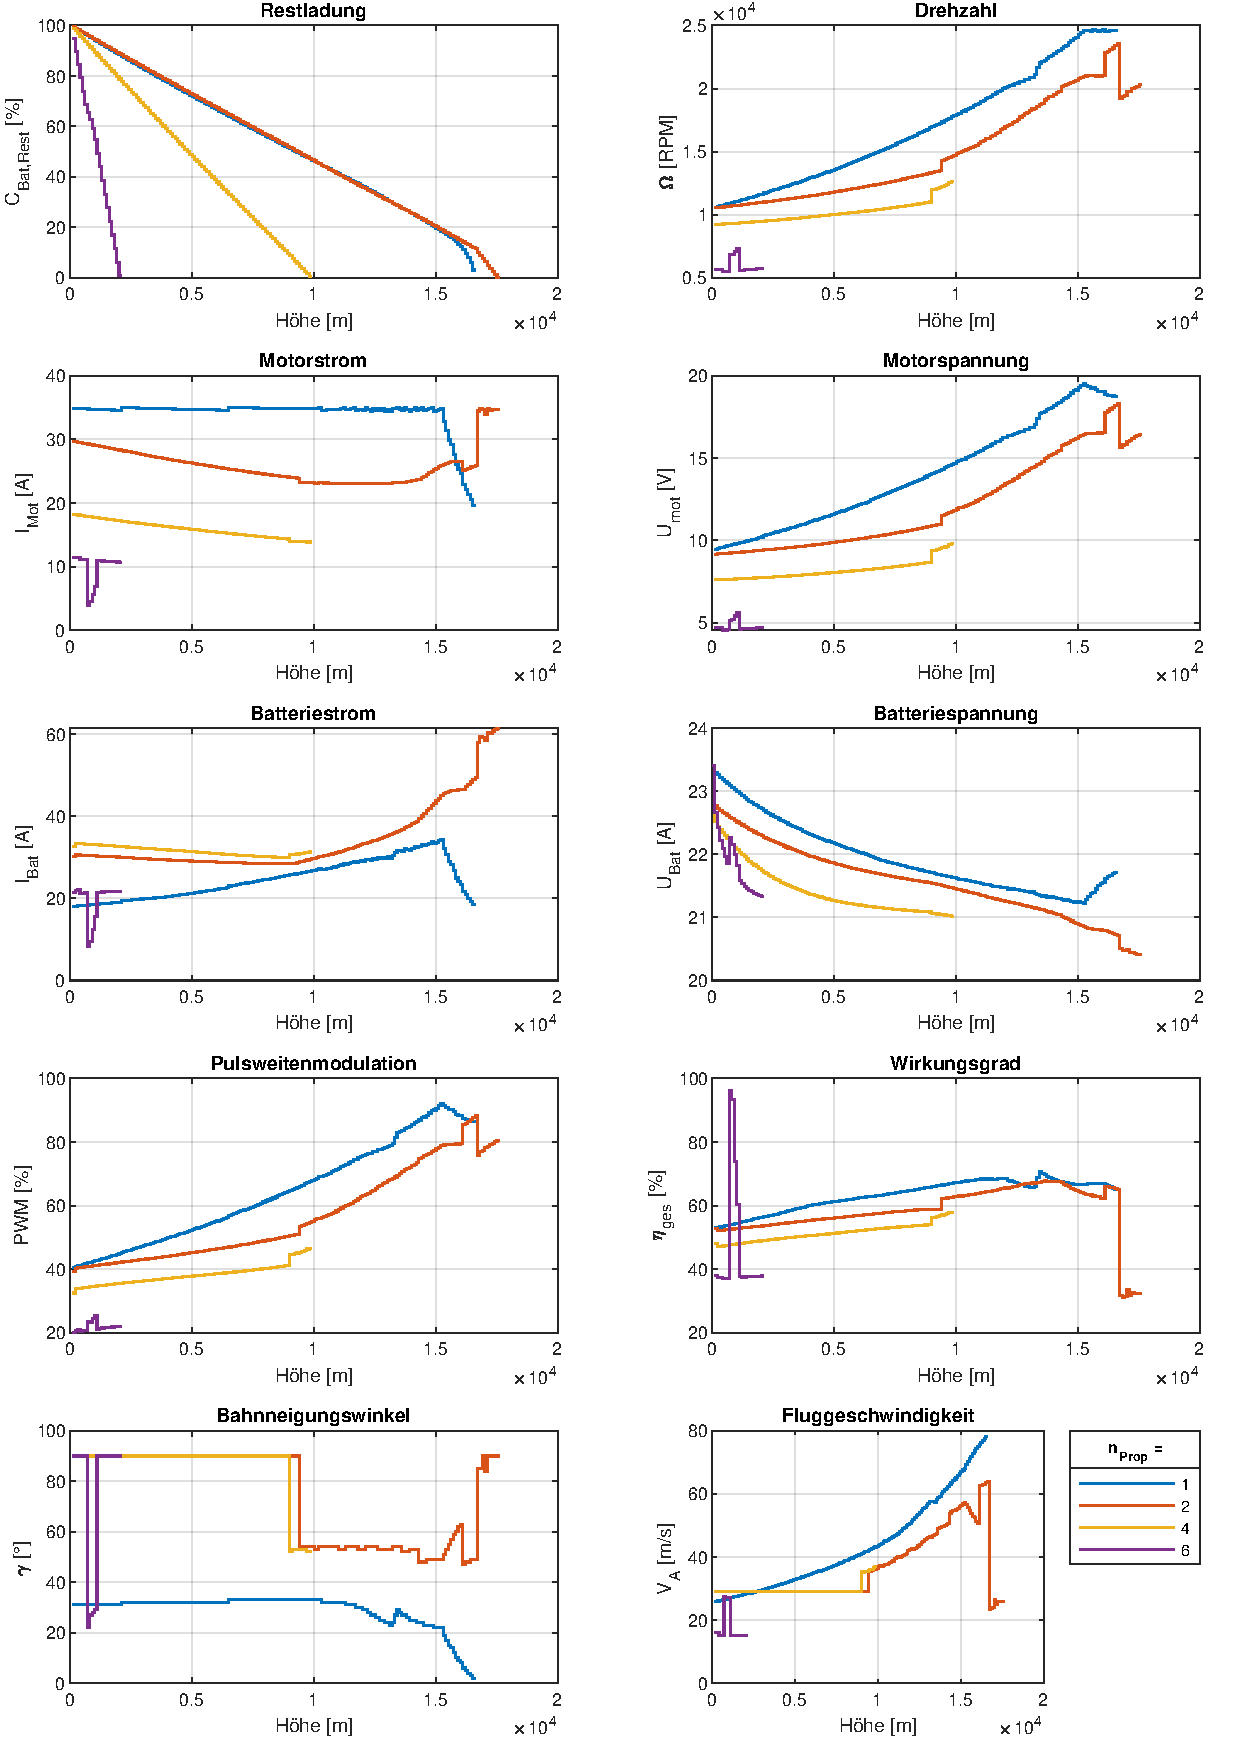
\includegraphics[scale=0.7]{Diagramme/Flaechenflzg_n_prop.pdf}
	\caption{Einfluss der Propelleranzahl auf die Flugleistungen eines Flächenflugzeugs (\ensuremath{m_{Mot}} = \SI{106}{g}, Propeller = 9x7)}
	\label{abb:flaechenflzg_mot_prop}
\end{figure}


\subsubsection{Gleitzahl}
Mit einer Verringerung der Gleitzahl geht auch eine Verringerung der maximalen Höhe mit einher und vice versa. Eine entsprechend hohe Gleitzahl beudeuted gleichzeitig auch eine entsprechend hohe aerodynamische Güte (Vgl. \cite[S.34]{Scheiderer.2008}). Dazu sinkt der Widerstand im Vergleich zum Auftrieb, sodass für ein Flächenflugzeug mit einer höheren Gleitzahl für den gleichen Auftrieb weniger Leistung zur Kompensation des Widerstandes aufgebracht werden muss. Als Konsequenz dessen steht mehr Leistung für das Steigen zur Verfügung. Mit der Gleitzahl steigt ebenso der optimale Steigwinkel. Als Grund dafür kann wieder die verringerte Widerstandsleistung angeführt werden. Zusätzlich sinkt die Zeit zum Überwinden einer Höhendifferenz mit steilerem Winkel. Einen Änderung der Gleitzahl hat nur einen Einfluss der auf die Restladung, die Batteriespannung und den Bahnneigungswinkel. Eine geringe Gleitzahl bedeutet einen stärkeren Einbruch der Batteriespannung, da wiederum im für den gleichen Auftrieb mehr Widerstand kompensiert werden muss. Auffällig ist noch Verbesserungszunahme der Flugleistungen mit der Gleitzahl. Diese Änderung ist im Bereich von 4 auf 10 deutich ausgeprägter als von 20 auf 50, obwohl dies mindestens einer Verdoppelung der Gleitleistung gleichkommt.
\begin{figure}[H]
\centering
	
\includegraphics[scale=0.7]{Diagramme/Flaechenflzg_E.pdf}
	\caption{Einfluss der Gleitzahl auf die Flugleistungen eines Flächenflugzeugs}
	\label{abb:gleitzahl}
\end{figure}


\subsubsection{Auslegungsgeschwindigkeit}
Die Auslegungsgeschwindigkeit hat einen bedeutenden Einfluss auf die erreichbare Höhe. Da für den Steigflug ein Flug mit konstanten Auftriebsbeiwert vorausgesetzt wird, erhöht sich aufgrund dessen die absolute Fluggeschwindigkeit mit der Höhe und größerem Bahnneigungswinkel (Vgl. Gleichung \ref{eq:geschw_flaechenflugzeug}).
Ist die Auslegungsgeschwindigkeit gering, so wächst sie absolut gesehen mit der Höhe nicht so stark wie hohe Geschwindigkeiten. Eine geringer gewählte Auslegungsgeschwindigkeit im Horizontalflug bedeutet daher auch, dass länger mit maximalen Motorstrom geflogen werden kann, bevor die Motorspannung die Batteriespannung erreicht und somit das Absinken des Steigwinkels einleitet.
Da mit der Auslegungsgeschwindigkeit auch die Geschwindigkeit mit der Höhe steigt, sind für hohe Geschwindigkeiten Propeller mit hohem Pitch vom Vorteil.
Ein Optimum zeichnet sich bei \SI{75}{km/h} aus. Es kann festgehalten werden, dass mit der Auslegungsgeschwindigkeit der Bahnneigungswinkel abnimmt, da die Steigzeit bei einer höheren Geschwindigkeit und geringerem Bahnneigungswinkel sich kaum ändert. Außerdem wird schneller \SI{100}{\%} PWM erreicht und damit gleichzeitig die Motorspannung begrenzt und der Flug mit maximalen Motorstrom beendet. Außerdem nimmt mit der Motorspannung der Zuwachs der Propellerdrehzahl ab. Weiterhin ist ein Zuwachs des Gesamtwirkungsgrades sowie der Bahngeschwindigkeit zu verzeichnen. Bei hohen Geschwindigkeiten begrenzt der mögliche Steigwinkel \ensuremath{\gamma} den Steigflug im Gegensatz zu der Begrenzung durch die Restladung bei niedrigen Auslegungsgeshwindigkeiten. Das schnelle Absinken von \ensuremath{\gamma} am Ende des  bedeutet für alle Auslegungen ein ineffizientes Manöver, da damit die Flugzeit für eine Höhenschritt ansteigt und auch einer deutlich höhere Energieentnahme der Batterie mit sich zieht.

\begin{figure}[H]
\centering
	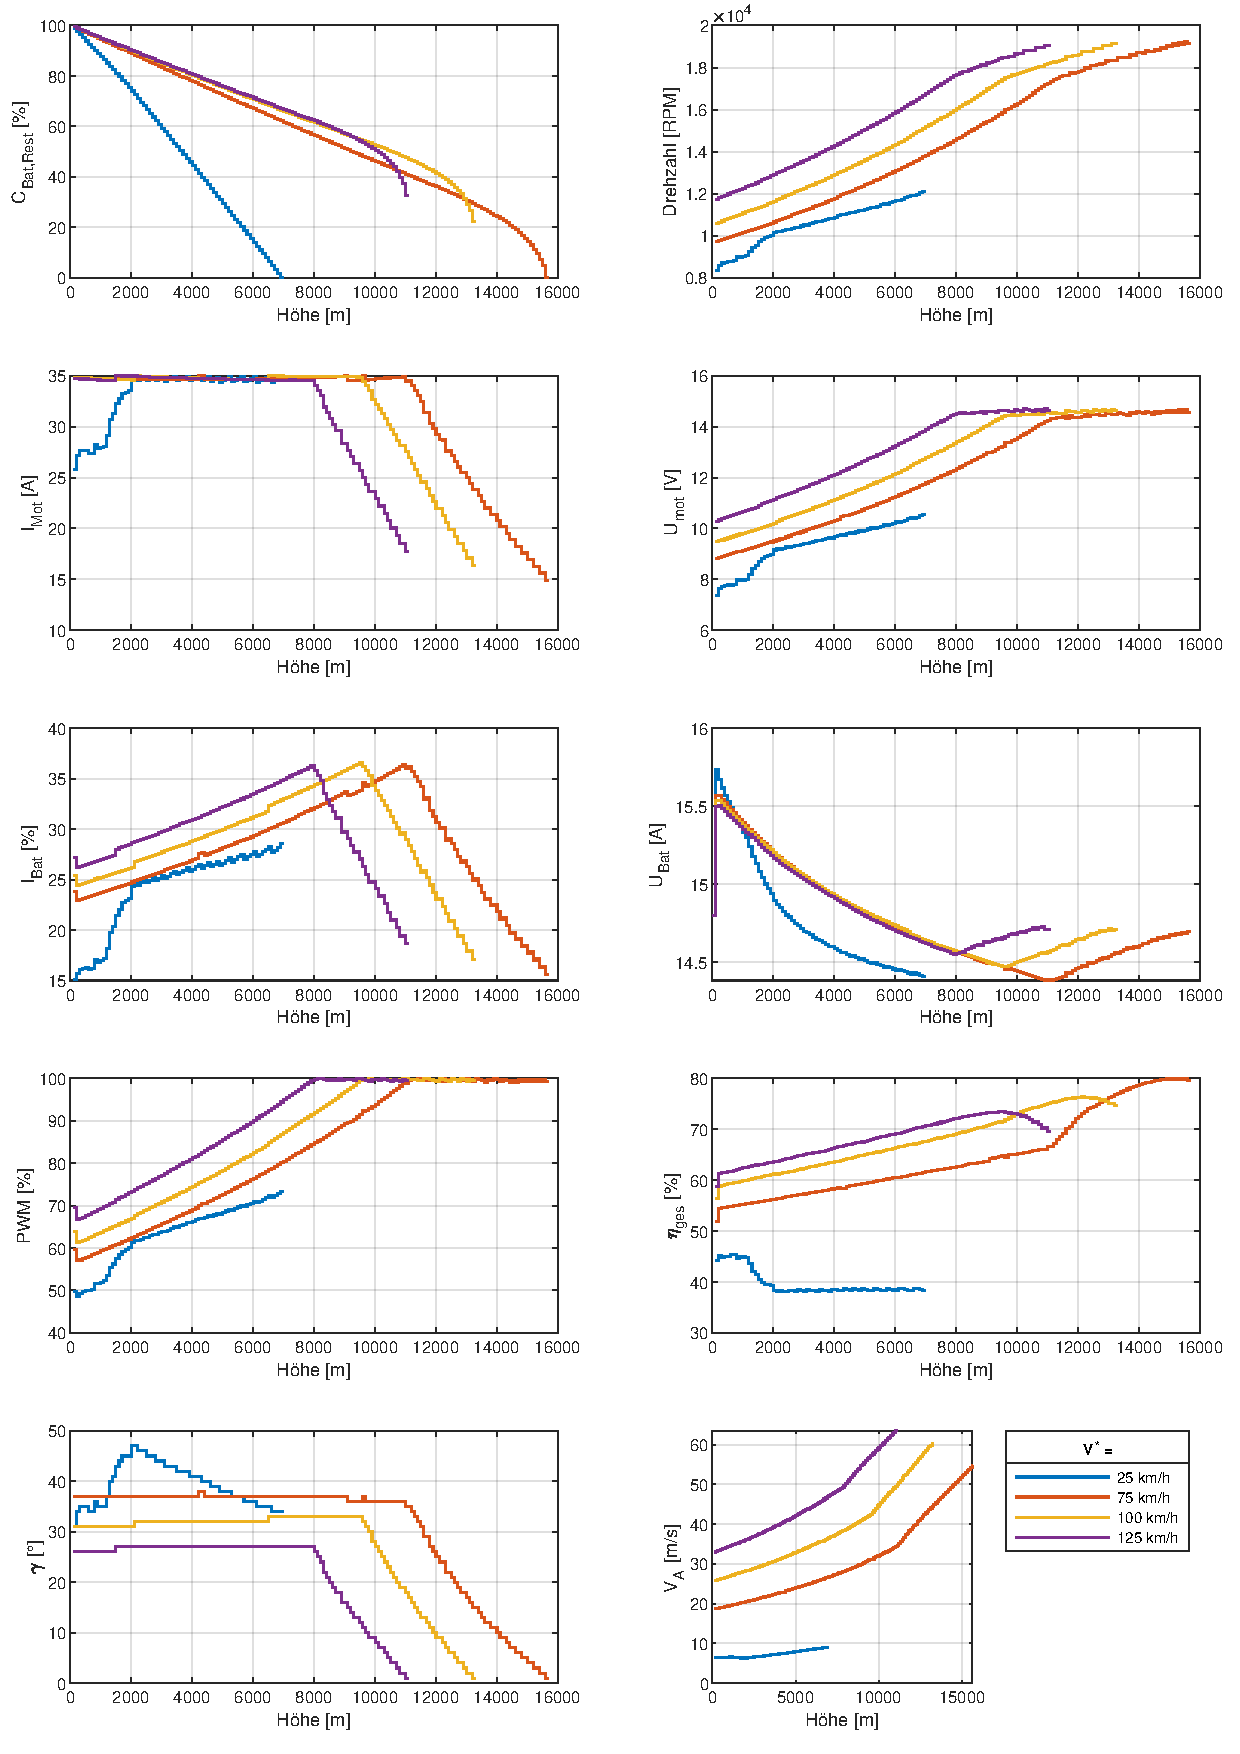
\includegraphics[scale=0.8]{Diagramme/Flaechenflzg_Vstern.pdf}
	\caption{Einfluss der Auslegungsgeschwindigkeit auf die Flugleistungen eines Flächenflugzeugs}
	\label{abb:vstern}
\end{figure}



\subsubsection{Penaltyfaktor}
Im Vergleich von einem Flächenflugzeug mit einem Multicopter muss bei gleichem Gesamtgewicht die unterschiedliche Verteilung der Gewichtskomponenten berücksichtigt werden. Für ein Flugzeug ist das Strukturgewicht von Flügeln und Rumpf sowie den Steuerungselementen bedeutend größer als das von einem Multicopter. Ein Penaltyfaktor von 1 entspricht daher wie oben beschrieben einer sehr optimistischen Einschätzung, wenn beide Strukturgewichte bei einem gleichen Gesamtgewicht äquivalent sind. Um realistischere Ergebnisse für ein Flächenflugzeug zu erreichen, wird der Penaltyfaktor schrittweise erhöht. Dabei verringert sich auch die maximal erreichbare Höhe. Dies hängt damit zusammen, dass ein Penaltyfaktor größer als 1 die zur Verfügung stehende Batteriemasse und folglich die Batteriekapazität reduziert.

\begin{figure}[H]
\centering
	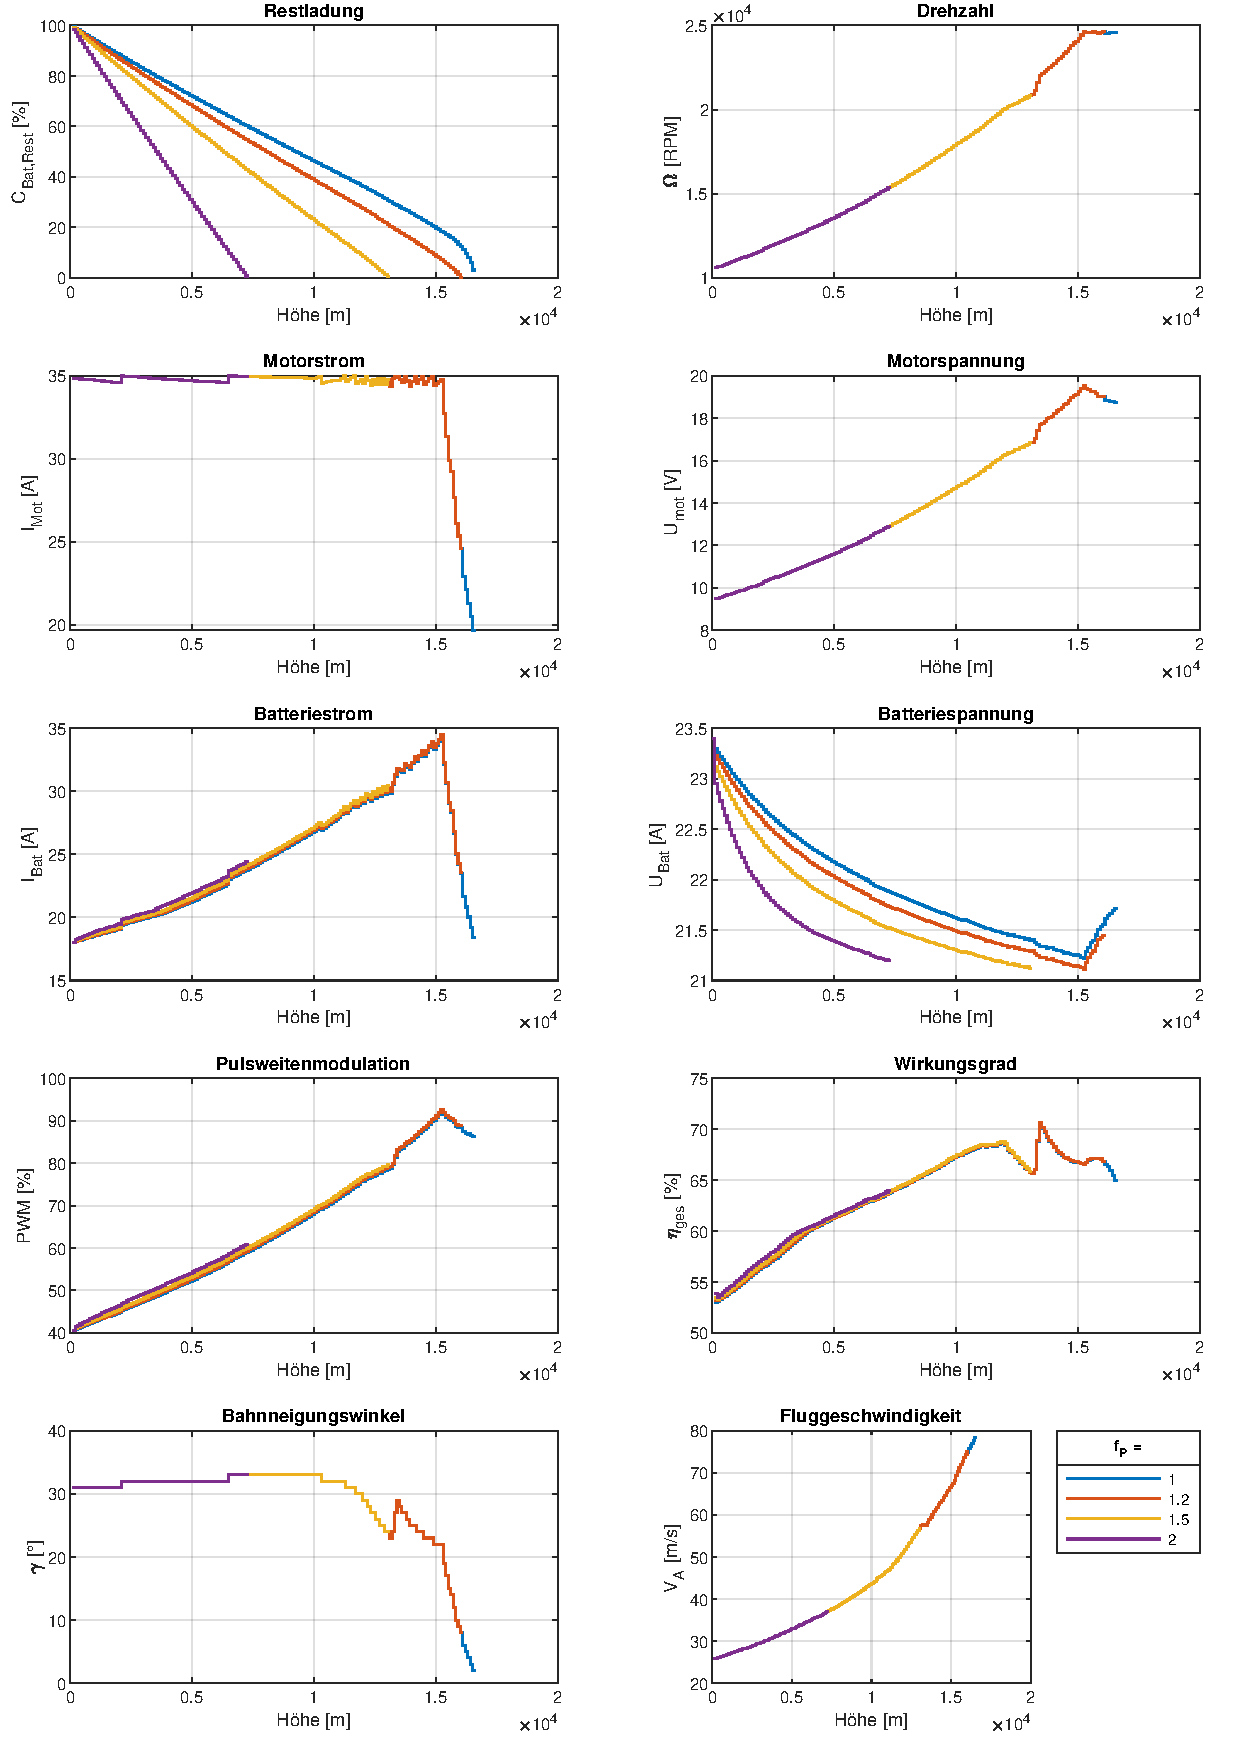
\includegraphics[scale=0.7]{Diagramme/Flaechenflzg_fp.pdf}
	\caption{Einfluss des Penalty-Faktors auf die Flugleistungen eines Flächenflugzeugs}
	\label{abb:fp}
\end{figure}


%\subsubsection{Motor-Propeller-Kombination}
%Die Motor-Propeller-Kombination beeinflusst entscheidend das Leistungsverhalten von elektrisch, propellergetriebenen Fluggeräten. Für jeden Motor werden vom Hersteller Propeller für einen bestimmten Anwendungsfall vorgegeben, mit dem optimale Leistungen erbracht werden können. Die Propellergröße hängt von der Leistung des Motors ab und von dem Auslegungsfall. Es zeigt sich, dass je stärker der Motor ist, desto größer ist der optimale Radius. Prinzipiell können auch kleinere Propeller verwendet werden. Aufgrund der Motorleistung ist der Pitch deshalb groß zu wählen, um den erforderlichen Schub zu liefern. Wird der Radius weiter vergrößert, so verringert sich der optimale Pitch. Außerdem sind Motoren mit niedrigen \ensuremath{K_V}-Werten bei gleichem Motorgewicht zu bevorzugen. Dies liegt in der Tatsache begründet, dass der \ensuremath{K_V}-Wert direkt den Motorstrom beeinflusst und ein hoher Wert diesen entsprechend zu Beginn des Fluges bereits stark erhöht. Zudem steht ein hoher \ensuremath{K_V} für eine hohe Maximaldrehzahl des Motors, aber für entsprechend weniger Drehmoment. Das gleiche gilt umgekehrt. 



%\subsubsection{Anzahl der Motoren}
%Noch bessere Ergebnisse können mit 2 Motoren erreicht werden, die  einen niedrigen \ensuremath{K_V}-Wert besitzen, aber ein hohes Leistungsgewicht. Mit dieser Konstellation sind Flughöhen bis zu \SI{15000}{m} möglich. In diesem Fall ist nicht der Flug mit maximalen Motorstrom am effizientesten sonder ein Flug mit konstantem Steigwinkel von ca. \SI{60}{^\circ}. Dabei sinkt der Motorstrom in diesem Zustand leicht, da das Drehmoment mit der Höhe abnimmt. Ebenfalls wie oben ist beschrieben ist dieser Zustand so lange fliegbar bis der Motorstrom auf dem Niveau des Batteriestroms und damit \SI{100}{\%} der PWM erreicht ist. Ab diesem Punkt steigt der Bahnneigungswinkel wieder an, da für einen Höhenschritt die Fluggeschwindigkeit mit Winkel sinkt. Alle anderen Größen verhalten sich analog zum oben beschriebenen Zustand. 
%Mit der Propelleranzahl verringert sich der Schub, der pro Propeller aufgebracht werden muss und damit auch die vom Motor benötigte Leistung. Folglich erhöht sich auch der Leistungsüberschuss. Dies resultiert auf der anderen Seite in einer höheren Belastung der Batterie.


\subsection{Ergebnisse des Vergleichs} 
Im direkten Vergleich weist das Flächenflugzeug eine größere maximale Flughöhe auf. Besonders mit hohen Gleitzahlen, mehreren Motoren und einer guten Kombination aus Motor und Propeller wird dieser Vorteil ersichtlich. Unter Berücksichtigung von zusätzlichen Widerständen und des einfachen Modells ist dieser Vorteil gerade wieder hinfällig sprich der zusätzliche Höhengewinn schwindet zu Null, wenn man die Widerstände berücksichtigt. Weiterhin erweist sich das Flächenflugzeug als bereits in den möglichen Maßen im Rahmen dieses Modells als optimiert. Die Steiggeschwindigkeit ist in Bezug auf den Auslegungszustand und einem Flug bei Auslegungsgleitzahl optimal. Außerdem wird der Steigwinkel für jeden Höhenabschnitt optimiert und eine gute Kombination von Motor und Propeller ist bereits gegeben. Schlussendlich ist damit der Spielraum für weitere Verbesserungen eingeschränkt. Hingegen zeigt der Quadrocopter in dieser Hinsicht noch Potenzial. Ein zu untersuchender Punkt ist noch die Abkehr von einer konstanten Steiggeschwindigkeit hin zu einer kontinuierlichen Optimierung dieser mit der Höhe. \\
Wird für das Flugzeug außerdem eine Konstellation von mehr als einem Motor gewählt, neigt das Flugzeug dazu in einem \SI{90}{^\circ} Winkel zu steigen. Damit zeigt sich die optimale Flugweise in einem vertikalen Steigflug. Hierbei werden nichtsdestotrotz wieder viel Vereinfachungen getroffen und Verluste nicht berücksichtigt. Die Vorteile eines Flächenflugzeuges zeigen sich auch nur stark bei einem Penalty-Faktor nahe bei 1. Dies muss als unrealistisch angesehen werden. Besonders im Bezug auf eine hohe Gleitzahl geht diese Anforderung mit einer hohen Flügelstreckung und damit mit einem hohen Strukturgewicht einher. Somit ist es zwingend notwendig den Penalty-Faktor zu erhöhen. Letztendlich verschwindet damit der Vorteil gegenüber einem Multicopter. 
In der Berechnung der Flächenflugzeugaerodynamik bleibt der Einfluss von Seitenwinden unberücksichtigt, da Seitenwinde nur die Strecke über Grund beeinflussen nicht aber die Flugeigenschaften im Steigflug (siehe Kap. \ref{subsubsec:schub_flaechenflzg}). Unter Berücksichtigung an das angedachte Operationsziel einer Atmosphärenmessung sind die Flugkorridore, die von der Deutschen Flugsicherung (DFS) zur Verfügung gestellt werden, begrenzt. Daher ist ein Abtrieb bei sehr hohen Seitenwinden für die Mission negativ und muss vom Fluggerät ausgeglichen werden. Dies verbraucht zusätzlich Energie zum Ausgleichen und reduziert nochmals die erreichbare Höhe. Dies geschieht beim Quadrocopter bereits durch den Ausgleich der Seitenwinde mit einer Anpassung vom Winkel \ensuremath{\alpha}, also einer Schrägstellung der Rotorebene. Ein weiteres Argument, was gegen den Einsatz von einem Flächenflugzeug spricht ist, dass eine Start und Landevorrichtung von Nöten ist. Das erfordert Platz für eine Start- und Landebahn. Dies entfällt für einen Quadrocopter aufgrund seiner Senkrechtstarterfähigkeiten. Es ist damit der Start von jeder beliebigen Stelle möglich.
Unter Berücksichtigung all dieser Fakten überwiegen die Vorteile beim Einsatz eines Multicopters. Dies gilt vor allem in Bezug auf das noch mögliche Potential eines Multicopters.


%\begin{itemize}
%	\item Ergebnisse 
%	\item ein Flächenflugzeug mit einem Motor erweist sich effizienter als
%ein Quadrocopter in Bezug auf die max. erreichbare Höhe
%	\item bei Vernachlässigung von zusätzlichen Widerständen und unter
%Berücksichtigung des einfachen Modells ist dieser Vorteil gerade
%wieder hinfällig sprich der zusätzliche Höhengewinn schwindet zu Null, wenn man die Widerstände berücksichtigt
%	\item weiterhin erweist sich das Flächenflugzeug als bereits in den möglichen Maßen optimiert (Steiggeschwindigkeit ist in Bezug auf Auslegungszustand und bei Auslegungsgleitzahl optimal, Steigwinkel wird optimiert, Auslegungsgeschwindigkeit und optimale Konstellation von Motor und Propeller
%	\item der Quadrocopter zeigt in diese Richtung noch Potenzial
%	\item bei der Erhöhung der Motoren- und damit auch Propelleranzahl neigt das Flugzeug dazu in einem 90° Winkel zu steigen, dabei optimiert sich die Steigeschwindigkeit bisher automatisch
%- eine Erhöhung der Gleitzahl erhöht die Anzahl der Ausreißer, quasi Abweichungen von dem 90° Zustand (zwischenzeitlich ist Flug mit 90° ernergieoptimaler, zwischenzeitlich der Gleitflug/ Steigflug mit geringerem Steigwinkel)
%	\item letztendlich führt die bisherige Untersuchung wohl zu dem Design eines VTOL-Fliegers (Vermutung)
%	\item wir haben weiterhin ein aerodynamisches Modell besprochen für einen VTOL-Flieger, Flugzustand bei entsprechendem Wind (Ausrichtung bspw. Messerflug) und Geschwindigkeitsmodell, entsprechend 4 mögliche Zustände (Steigwinkel anpassen, Steigwinkel und Fluggeschwindigkeit aus der Gleichungssystem lösen, etc.)
%	\item ich werde nun den Multicopter weiter untersuchen (Anpassung der Steiggeschwindigkeit, Gewicht, Größe, etc.)
%	\item als unterer Ast des Baumes ist eine Untersuchung der Verkleidung des Copters in Richtung VTOL-Flugzeug interessant,folglich auch weitere Untersuchung in diese Richtung

%\end{itemize}

%******************************************************************

\section{Steiggeschwindigkeit}
\label{sec:steiggeschwindigkeit}
Eine weitere Optimierung des Multicopters bzw. des Quadrocopters kann durch eine Anpassung der Steiggeschwindigkeit geschehen. Die vormalig als konstant angenommene Steiggeschwindigkeit von \SI{10}{m/s} (Kap. \ref{chap:nachbildung}) ist nicht in jedem Operationspunkt optimal. Die Steiggeschwindigkeit wird wieder für jeden Höhenschritt variiert. Analog zur Variation des Steigwinkels beim Flächenflugzeug fällt die Auswahl der Geschwindigkeit auf den Wert, welcher die geringste Energiemenge benötigt für den Aufstieg. Bei der Untersuchung kristallisieren sich drei starke Einflussfaktoren heraus. Im Einzelnen sind das der Widerstandsbeiwert, die Anzahl der Batteriezellen und die Motorleistung. Im Abb. \ref{abb:steiggeschw} ist der Ablauf der Leistungsberechnung für die Steiggeschwindigkeit dargestellt. In diesem Abschnitt werden die oben genannten Parameter an der Konstellation aus (Kap. \ref{chap:nachbildung}) untersucht, da dies den Einfluss sehr gut verdeutlicht.


\subsection{Ergebnis}
Mit einer variablen Steiggeschwindigkeit ist ein deutlicher Höhengewinn von \SI{3000}{m} zu verzeichnen. Die Steiggeschwindigkeit liegt deutlich über den \SI{10}{m/s}, die vorher angenommen wurden. Mit einer höheren Steiggeschwindigkeit sinkt auch die Flugzeit und als Konsequenz auch die benötigte Kapazität für einen Höhenschritt. Auf der anderen Seite steigt mit einer größeren Fluggeschwindigkeit die Widerstandskraft quadratisch an (Vgl. Gleichung \ref{eq:widerstand}. Dies wird noch genauer in Kap. \ref{subsec:widerstandseinfluss} beschrieben. 

\begin{figure}[H]
\centering
	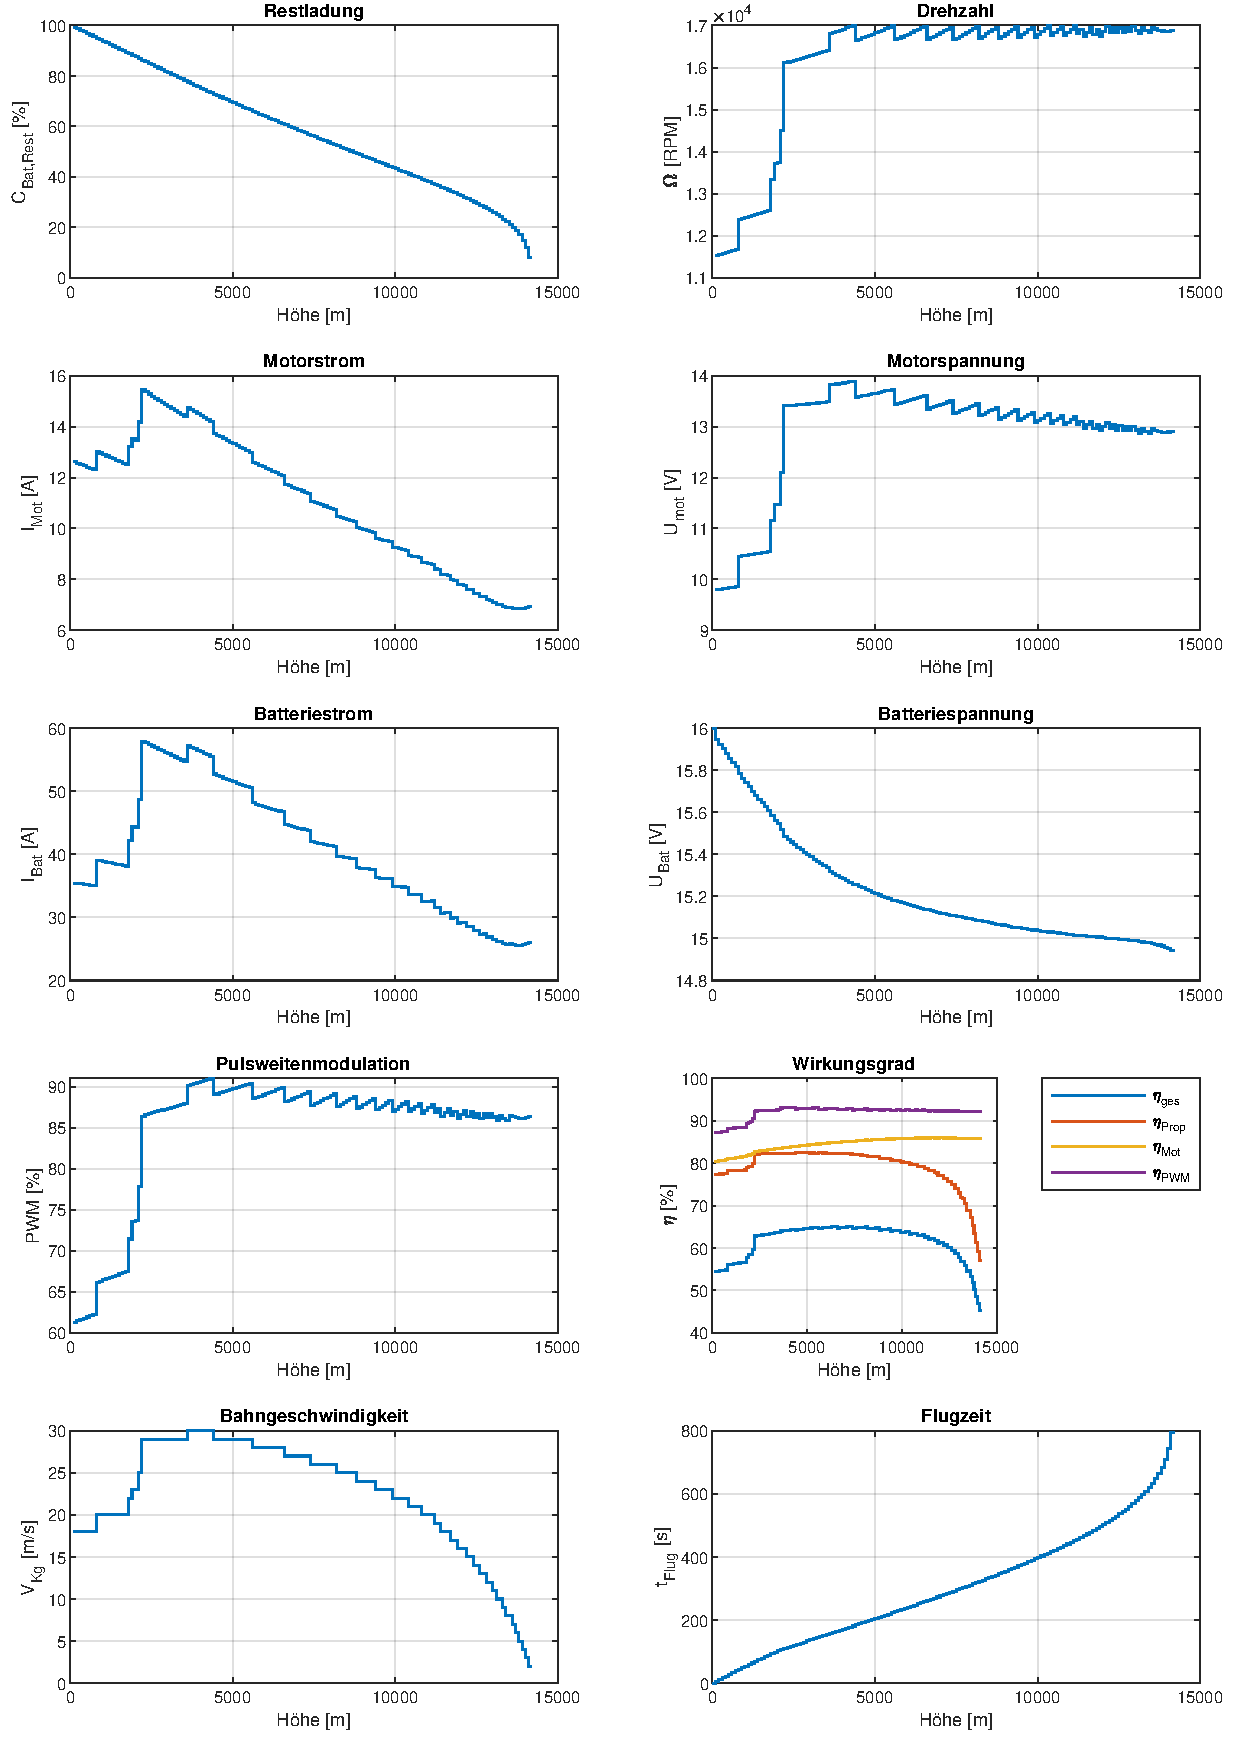
\includegraphics[scale=0.7]{Diagramme/Russland_vvar.pdf}
	\caption{Flugleistungen des Quadrocopter aus \cite{Anderson.2018} mit variabler Steiggeschwindigkeit}
	\label{abb:fp}
\end{figure}


\subsection{Einfluss des Widerstands}
\label{subsec:widerstandseinfluss}
Der Widerstandsbeiwert hat einen entscheidenden Einfluss auf die maximale Steiggeschwindigkeit. Bei einem großen maximalen Motorstrom gilt, dass die Begrenzung der Geschwindigkeit durch den Widerstandsbeiwert erfolgt. Eine sehr hohe Geschwindigkeit verringert zum einen die Flugzeit für einen Höhenbereich, erhöht auf der anderen Seite jedoch den Widerstand und damit zusätzlich die benötigte Leistung. Je geringer der \ensuremath{C_W} gewählt wird, desto höher ist die optimale Steiggeschwindigkeit. Erhöht sich im Umkehrschluss der Luftwiderstand so sinkt die Steiggeschwindigkeit, da der Widerstand mit der Geschwindigkeit quadratisch (Vgl. Gleichung \ref{eq:widerstand}) ansteigt. Im Sinne einer großen maximalen Höhe ist daher eine aerodynamisch günstige Verkleidung des Multicopters anzustreben.
  
\begin{figure}[H]
\centering
	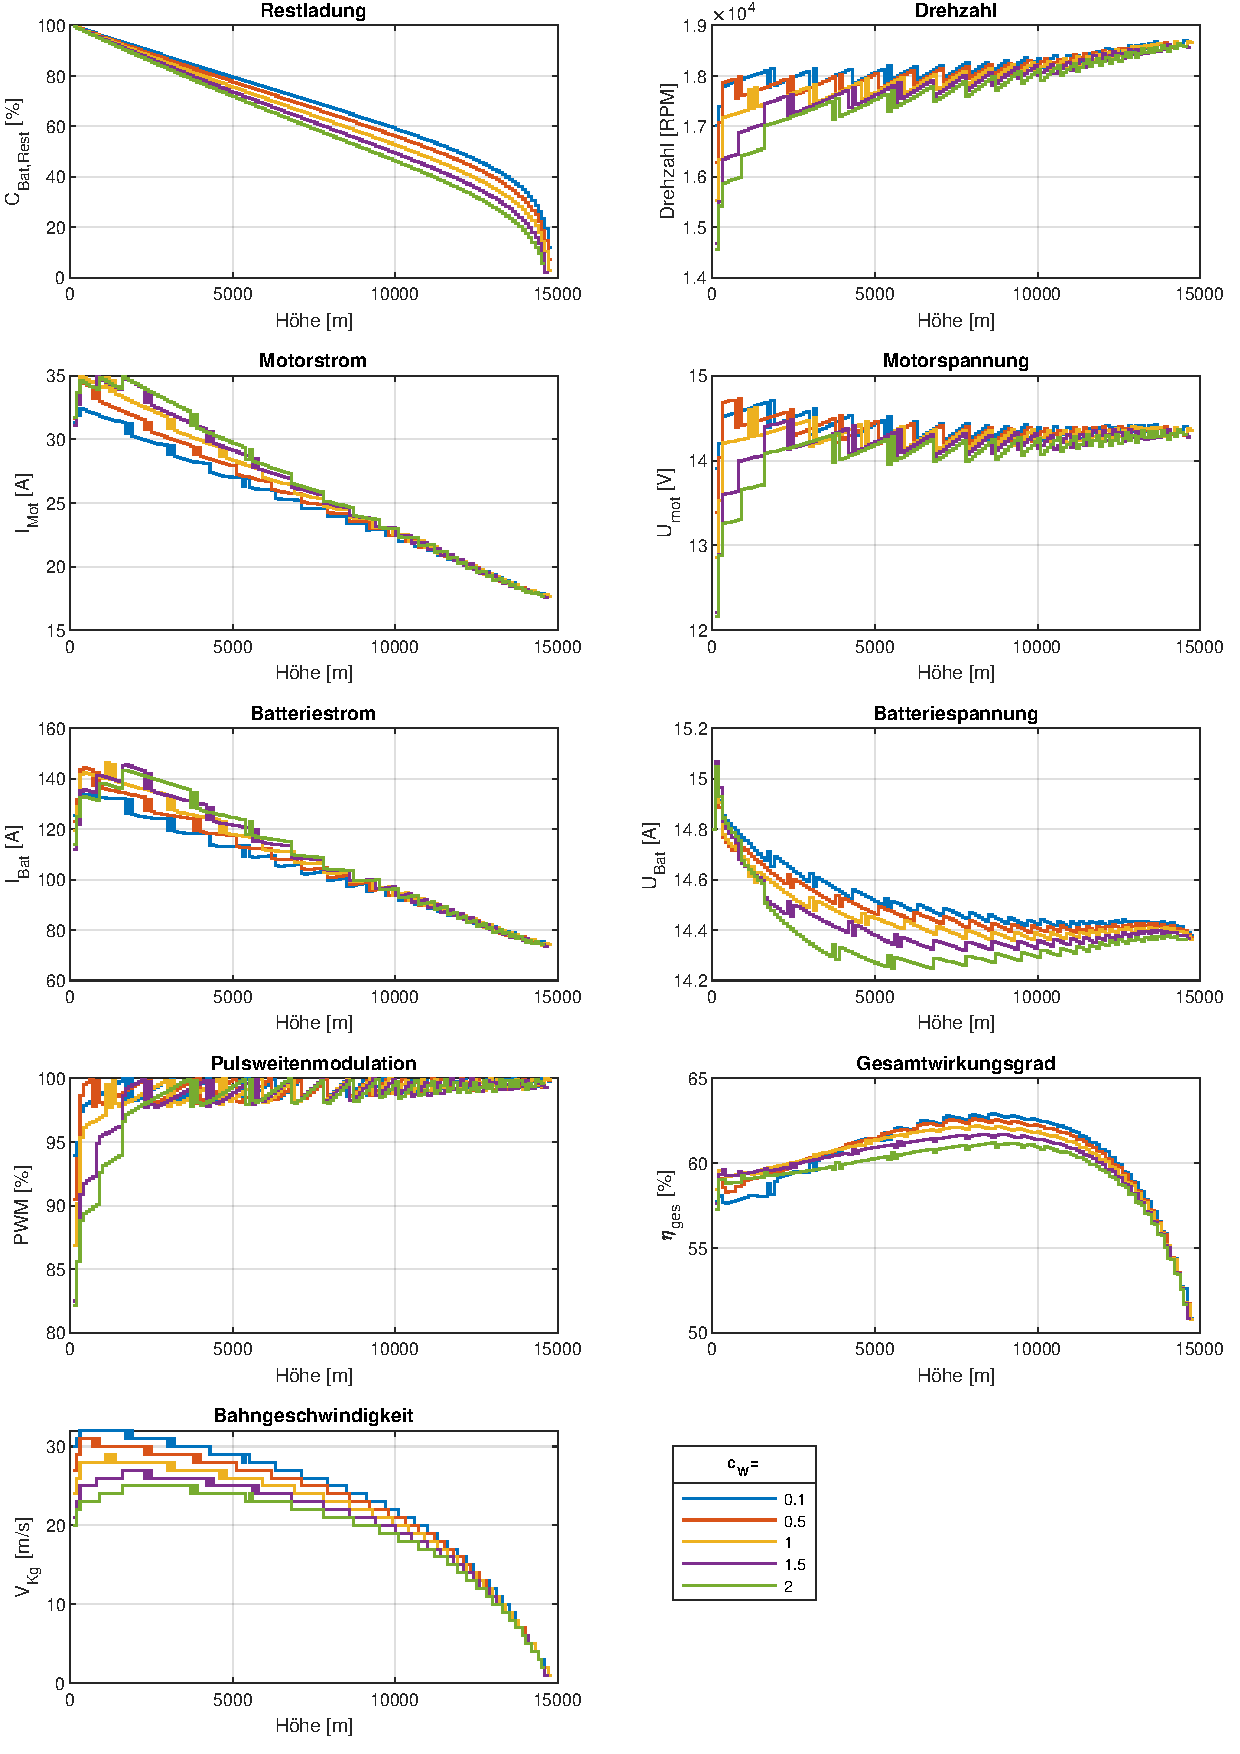
\includegraphics[scale=0.7]{Diagramme/Untersuchung_c_W.pdf}
	\caption{Widerstandseinfluss auf die maximale erreichbare Höhe}
	\label{abb:c_W_einfluss}
\end{figure}

%\begin{itemize}
%	\item der Widerstandsbeiwert hat einen entscheidenden Einfluss auf die maximale Steiggeschwindigkeit
%	\item prinzipiell gilt bei einem großen maximalen Motorstrom, dass die Begrenzung der Geschwindigkeit durch den Widerstandsbeiwert erfolgt. Eine sehr hohe Geschwindigkeit verringert zum einen die Flugzeit für einen Höhenbereich, erhöht auf der anderen Seite jedoch den Widerstand und damit die benötigte Leistung. 
%	\item je geringer der \ensuremath{C_W} gewählt wird, desto höher die Steiggeschwindigkeit, da der Widerstand bei großen Werten noch einen geringen Einfluss hat
%	\item Eine Erhöhung von diesem bezweckt eine Erhöhung eine Verringerung der optimalen Fluggeschwindigkeit
%	\item auch hier gilt wieder, dass der Flug mit \SI{100}{\%} am effizientesten ist
%\end{itemize}

\subsection{Einfluss der Anzahl der Batteriezellen}
\label{subsec:einfluss_n_bat}
Ein weiterer begrenzender Parameter ist die PWM. Die Motorspannung an sich kann nicht beeinflusst werden. Jedoch lässt sich Einfluss auf die Höhe der Motorspannung durch eine Erhöhung der in Reihe geschalteten Batteriezellen nehmen. Mit jeder zusätzlichen Zelle erhöht sich die nominelle Batteriespannung um \SI{3,7}{V}. Damit stellt die PWM nicht mehr die Grenze für die Steiggeschwindigkeit dar. Der effizienteste Flugzustand ist nun der bei maximalen, dauerhaften Motorstrom. Jedoch führt bei gleicher Energiemenge 
\begin{equation}
	E_{Bat} = C_{Bat}\cdot U_{Bat}
\end{equation}
eine Erhöhung der Spannung in dem Produkt aus Spannung und Kapazität (\ensuremath{C_{Bat} = I_{Bat}\cdot t_{Flug}}) unweigerlich zu einer Verringerung der Kapazität. Die schlägt sich wieder auf den Kostenfaktor aus, der erreichbaren Flughöhe. Diese Maßnahme ist also mit Bedacht zu wählen. Eine extreme Erhöhung der Zellenanzahl bewirkt außerdem wieder ein Flug mit maximalen Motorstrom.
Die schlechtesten Flugleistungen weist die Batterie mit nur zwei Zellen auf. Diese kann nur eine geringe Batteriespannung liefern, weshalb die maximale Drehzahl, der maximale Motorstrom und die -spannung und schließlich auch die Bahngeschwindigkeit sehr niedrige Werte aufweisen. Dies kann mit der sehr niedrigen Batteriespannung begründet werden. Das Ende des Steigfluges ist erreicht, wenn die Steiggeschwindigkeit null erreicht und die Batterie nicht mehr die erforderliche Spannung für ein weiteres Steigen zur Verfügung stellen kann. Durch die Motorspannung ist die maximale Motordrehzahl begrenzt und damit die Propellerdrehzahl (Vgl. Gleichung \ref{eq:motorspannung}, sodass der vom Propeller erzeugte Schub mit der Höhe abnimmt.\\
Deutlich bessere Ergebnisse liefert eine Verdoppelung der Zellenanzahl auf vier. Bei dieser ist auch sofort die Pulsweitenmodulation auf \SI{100}{\%} angestiegen, allerdings ist die nominale Spannung doppelt so hoch. Dies folgert eine höhere Drehzahl, höhere Motorkenngrößen, einen deutlich verbesserten Gesamtwirkungsgrad und einen schnelleren Steigflug. Auch diese Konstellation endet analog zur Batterie mit nur zwei Zellen mit dem Absinken der Bahngeschwindigkeit gegen null durch den verringerten Propellerschub. \\
Die Leistungsparameter für die sechs- und achtzellige Batterie sind in Bezug auf die Restladung die Propellerdrehzahl, den Motorstrom und die -spannung sowie die Bahngeschwindigkeit beinahe identisch. Lediglich in den Batteriekenngrößen und damit auch in PWM treten Unterschiede auf, weil mit der Zellenanzahl die nominelle Batteriespannung steigt und damit die PWM sinkt (Vgl. Gleichung \ref{eq:pwm}). Der Batteriestrom nimmt ebenfalls ab. 
Ein wichtiger Punkt ist hier noch der Gesamtwirkungsgrad. Dieser fällt ebenfalls mit der nominellen Batteriespannung. Insbesondere für die Batterien mit sechs und acht Zellen sind der Propeller- und Motorwirkungsgrad identisch, da die Leistungsgrößen, die auf diese Wirkungsgrade einen Einfluss haben, enbenfalls identisch sind. \\
Der Grund unterschiedlichen Gesamtwirkungsgrade liegt im Wirkungsgrad des Motorreglers. Ein sinkende PWM erhöht die Verluste und verringert den Wirkungsgrad (Vgl. Gleichung \ref{eq:eta_pwm}). Dies soll in Abschn. \ref{subsec:einfluss_eta_pwm} genauer untersucht werden.


\begin{figure}[H]
\centering
	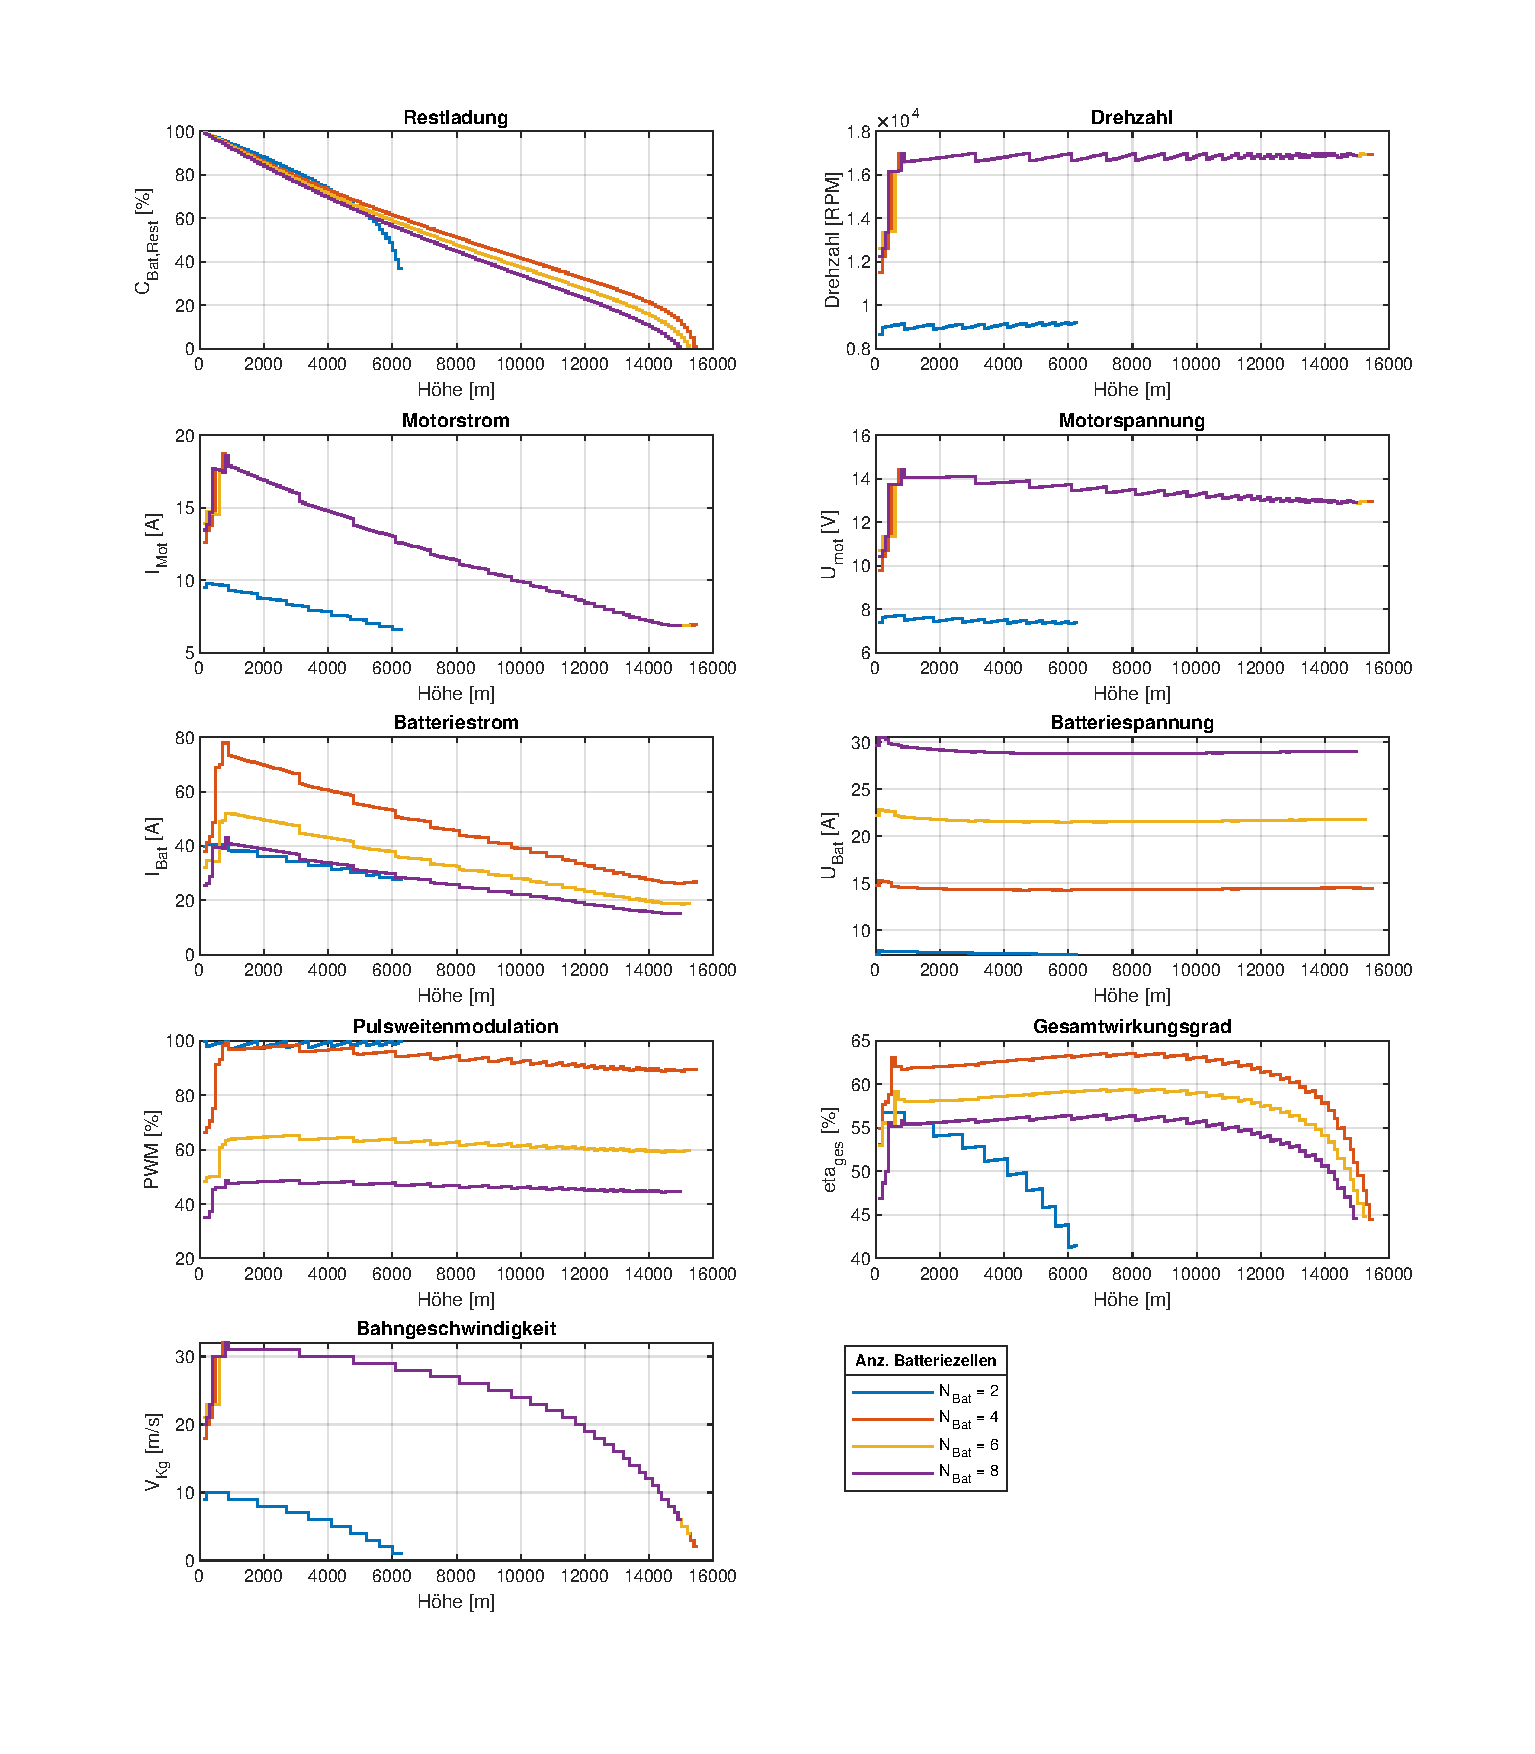
\includegraphics[scale=0.70]{Diagramme/Untersuchung_N_Bat.pdf}
	\caption{Einfluss der Batteriezellenanzahl auf die maximale erreichbare Höhe}
	\label{abb:N_Bat_einfluss}
\end{figure}

\subsection{Bedeutung des Reglerwirkungsgrades}
\label{subsec:einfluss_eta_pwm}
Der Wirkungsgrad des ESC ist ausschließlich eine Funktion der PWM (Vgl. Gleichung \ref{eq:eta_pwm}). Wie bereits in Abschn. \ref{subsec:einfluss_n_bat} erklärt, sinkt die PWM mit der Erhöhung der Batteriezellenanzahl. Zeitgleich steigen die Verluste in diesem ESC-Modell. Im Sinne eines besseren Gesamtwirkungsgrades und der erreichbaren Höhe ist eine Verringerung der Reglerverluste anzustreben. Die Ergebnisse sind in \ref{sec:motorreglerwirkungsgrad} dargelegt. \\
Insgesamt ist der Einfluss des Reglerwirkungsgrades sehr gering. Mit dem ESC-Wirkungsgrad steigt auch der Gesamtwirkungsgrad deutlich und auch die Restkapazität. Auf die maximale Höhe ist dieser Einfluss allerdings unbedeutend. Der zusätzliche Höhengewinn macht ungefähr \SI{100}{m} aus.



\subsection{Einfluss des maximalen Motorstroms}
Die Ergebnisse zeigen, dass ein geringer maximaler Motorstrom ebenfalls die Steiggeschwindigkeit begrenzt. Dieser begrenzt die dem Motor entnommene Leistung. 
Folglich ist ein Motor für einen solchen Steigflug zu wählen, der einerseits einen hohen \ensuremath{K_V}-Wert besitzt, andererseits aber auch einen hohen maximalen Dauerstrom besitzt (Vgl. Kap. \ref{subsubsec:mot_prop_kombi}). Ein gutes Beispiel ist der Motor aus Kapitel \ref{subsubsec:mot_prop_kombi} mit einem \ensuremath{K_V}-Wert von \SI{2850}{RPM/V} und einem maximalen Motorstrom \ensuremath{I_{max}} von \SI{55}{A}.



%******************************************************************

\section{Massenverteilung}
\label{sec:massenverteilung}
Ein weiterer wichtiger Punkt, der an dieser Stelle untersucht werden soll, ist die Massenanteilsverteilung von den Motoren, der Batterie und der Leermasse des Multicopters am Gesamtgewicht. Wiederum stellt der Quadrocopter aus Kapitel \ref{sec:komponenten} die Grundlage der Untersuchung dar. Bei diesem nehmen die Motoren \SI{13,77}{\%}, die Batterie \SI{52,83}{\%} und die der Rahmen mit den übrigen Komponenten \SI{33,4}{\%} der Gesamtmasse von \SI{1060}{g} ein. Für einen Gegenvergleich wird nun ein anderen Quadrocopter mit diesen Massenverhältnissen erstellt. Als Anhaltspunkt dient die Masse der Motoren, da diese durch die Datenbank vollständig definiert sind und eine feste Masse besitzen. Alle anderen Massenverteilungen ergeben sich im Anschluss aus der Motormasse.
Die Massen errechnen sich nach folgendem Schema:
\begin{align}
	m_{ges} &= \frac{n_{Prop}\cdot m_{Mot}}{0.1377} , \\
	m_{Bat} &= m_{ges}\cdot 0.5283 , \\
	m_{copter} &= m_{ges}\cdot 0.334.
\end{align}
Zusätzlich wird jeweils auch die obere Stirnfläche \ensuremath{A_{copter,oben}} mit der Größe angepasst. Im folgenden wird die Masse der Batterie 

\subsection{Ergebnisse}
\label{subsec:ergebnis_massenverteilung}
\newpage
\begin{figure}[H]
\centering
	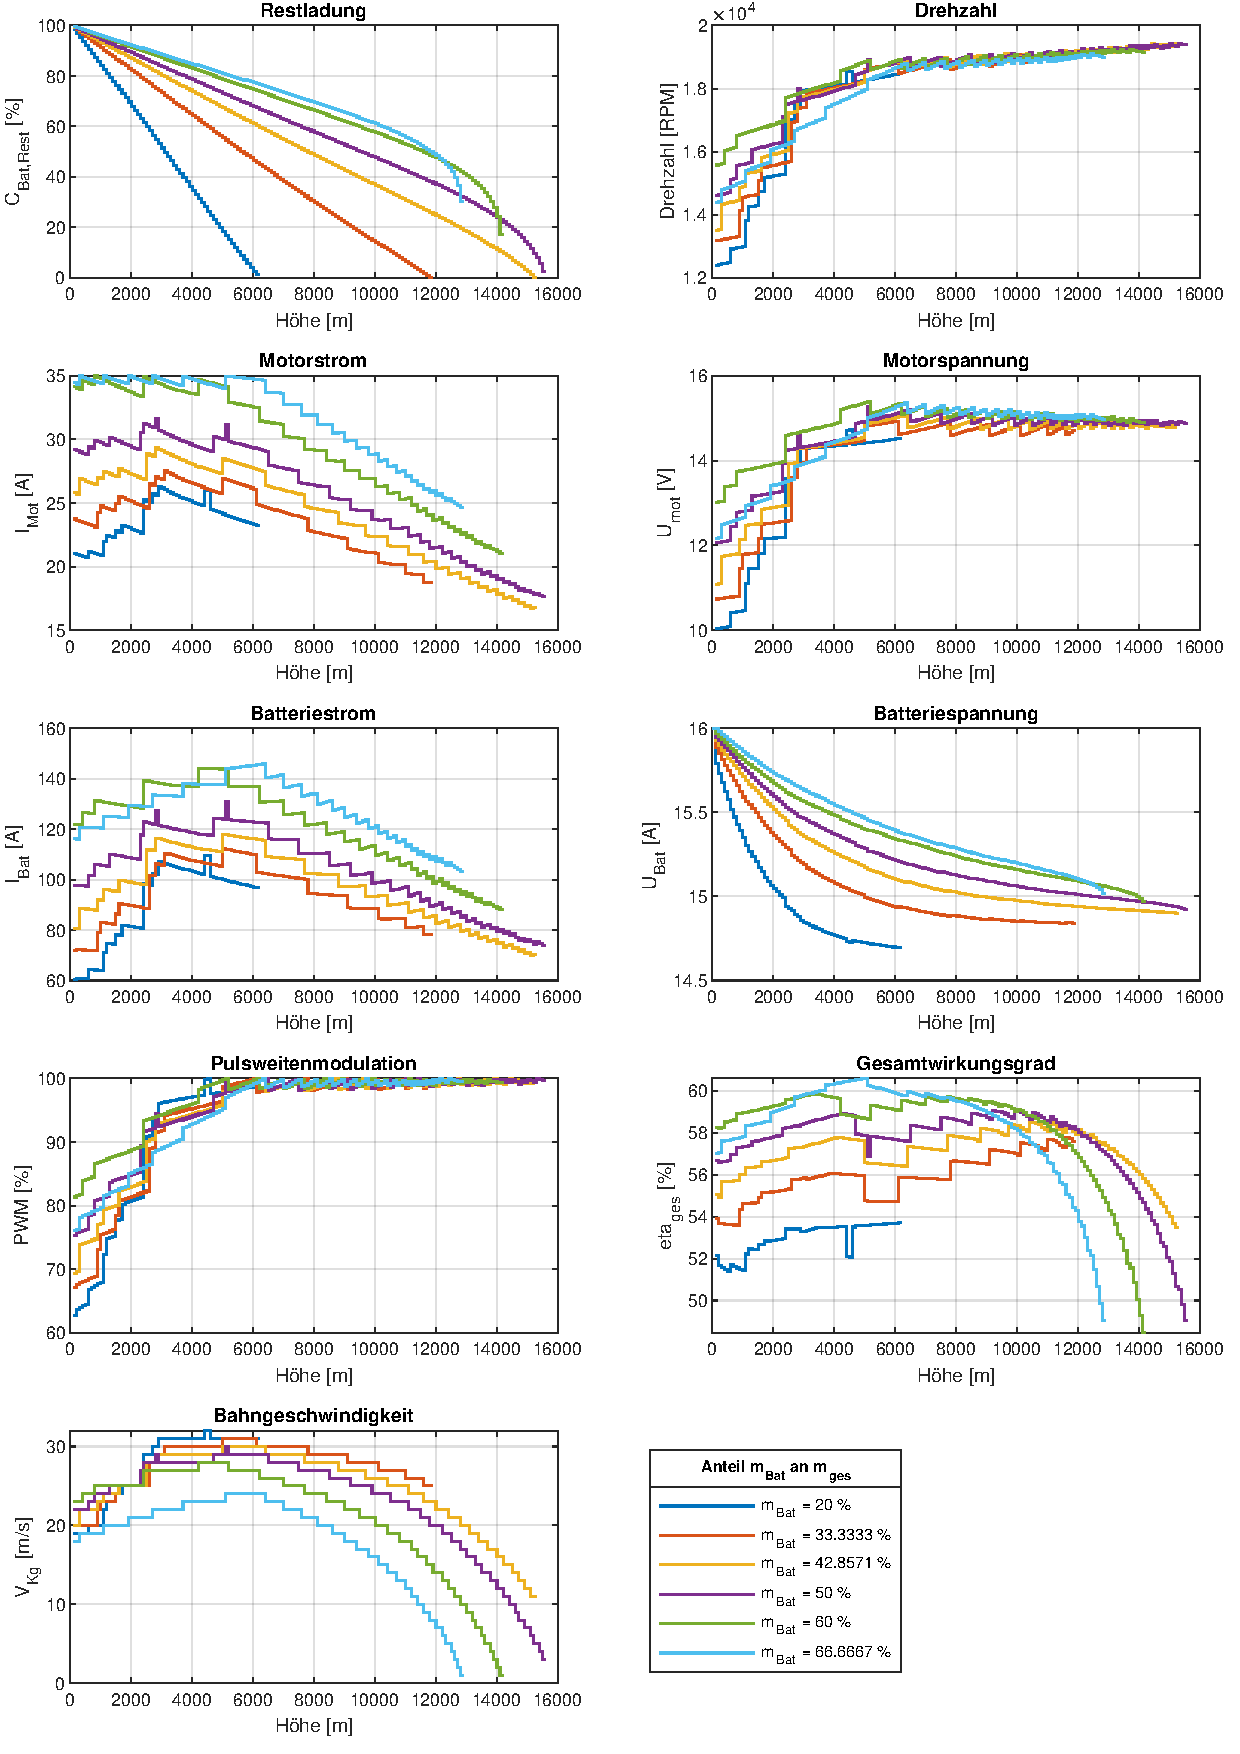
\includegraphics[scale=0.70]{Diagramme/Batteriemasse.pdf}
	\caption{Abhängigkeit der maximalen Höhe von Batteriemasse anteilig an der Gesamtmasse (\ensuremath{m_{Mot}=\SI{106}{g}}, \ensuremath{K_V=\SI{1390}{RPM/V}}, \ensuremath{n_{Prop}=4}, \ensuremath{Propeller=\SI{10x3}{}}, \ensuremath{n_{Bat,cell}=4}, \ensuremath{u_{Wg}=\SI{10}{m/s}})}
	\label{abb:batteriemasse}
\end{figure}

Die Batteriemasse hat einen großen Einfluss auf die Flugleistungen. Die TOC's variieren zwischen eine Spanne von \SI{5000}{m}. Ein Optimum ist bei einer Konstellation erreicht, bei der die Batteriemasse die Hälfte des Gesamtgewichts ausmacht also \SI{50}{\%}. Die Kurven der Restladungskurven von \SI{60}{\%} und \SI{66.66}{\%} sind bis zu einer Höhe von \SI{12500}{m} deckungsgleich. Danach reduziert sich die Restladung eines Fluggeräts mit einem höheren Anteil der Batteriemasse drastisch. Mit einem zunehmenden Batteriemassenanteil ist für den Steigflug nicht mehr die Kapazität der Batterie begrenzend sondern vielmehr die Leistung und der vom Propeller erzeugte Schub (indirekt damit auch die Fluggeschwindigkeit). Mit zunehmender Batteriemasse reduziert sich auch die Bahngeschwindigkeit signifikant. Dies liegt darin begründet, dass die Masse direkt in den Schub mit einfließt (Vgl. Gleichung \ref{eq:neigungswinkel} und \ref{eq:schub_multicopter}). Ein schlechte Verteilung der Massen erhöht somit den Schub und damit die erforderliche Leistung für eine feste Verteilung von Motor- und Multicoptermasse. 
eine zu geringe Masse und damit Kapazität der verringert zum einen die erforderliche Motorleistung (Vgl. Niveau des Motorstroms und Spannung in Abb. \ref{abb:batteriemasse}), allerdings ist die Kapazität . 


Dies beeinflusst die Bahngeschwindigkeit, welche die Flugzeit und letztendlich die erreichbare Höhe bestimmt. Weiterhin kann mit größeren Batteriemassen länger mit maximalen Motorstrom geflogen werden, bevor die PWM \SI{100}{\%} erreicht und die Steiggeschwindigkeit sinkt, \textcolor{red}{da das maximale Niveau leistungsbedingt nicht mehr gehalten werden kann.} Für kleinere Batteriemassen beginnt der Flugabschnitt mit \SI{100}{\%} PWM bereits deutlich früher (pro \SI{25}{\%} mehr Batteriemasse sind das ungefähr zusätzliche \SI{2500}{m} Höhe). Dies hat zur Folge, dass die maximale Drehzahl (ca. \SI{19000}{RPM}) früher erreicht ist. Durch die großen Steiggeschwindigkeiten bei kleinen Batteriemassen ist auch ein deutlich stärkerer Einbruch der Batteriespannung zu verzeichnen (ca.\SI{1,25}{V} bei \SI{20}{\%} und nur \SI{1}{V} bei größeren Massenanteilen). Zudem ist analog zu den Kurven der Restladung bei den optimalen Konstellationen auch der optimale Gesamtwirkungsgrad erreicht. Die optimale Batteriemasse liegt zwischen \SI{50}{\%} und \SI{52.5}{\%} (Vgl. Anhang).
Dies widerspricht den Aussagen von \cite{Neitzke.2013}, worin die besten Flugleistungen und insbesondere die längste Flugdauer mit einem Anteil der Batteriemasse an der Gesamtmasse von 2/3 angegeben wird. Ein möglicher Grunde sind die unterschiedlichen Flugzustände. Neitzke hat seine Untersuchungen ausschließlich im Hovern gemacht. Somit fehlt in seinen Betrachtungen der Höheneinfluss und der Einfluss einer Steiggeschwindigkeit. \textcolor{red}{Neitzke nimmt einen konstanten Wirkungsgrad für alle an, was aber nicht für alle Flugzustände gilt.}\\
Zusammengenommen weisen die obige Untersuchung der Massenverteilung und der Quadrocopter aus Russland das gleiche Ergebnis auf. Die Konstellation des Quadrocopters aus \cite{Anderson.2018} erweist sich bereits in diesem Sinne als optimal.\\
Es ist außerdem ersichtlich, dass die Flugleistung und -dauer noch weiter verbessert werden können, wenn der Massenanteil des Rahmens und aller übriger kleiner wird und die Masse der Batterie im Gegensatz steigt, i.e. eine Tendenz der Coptermasse gegen Null (\ensuremath{m_{Copter}\rightarrow 0} und \ensuremath{m_{Bat}\rightarrow (m_{Bat}+m_{Copter})})


%******************************************************************

\section{Größe und Anzahl der Propeller des Fluggerätes}
\label{sec:groesse}
Ein weitere Einfluss auf die Flugleistungen stellt das Gesamtgewicht des Fluggerätes dar. Dabei wird das Fluggerät äquivalent skaliert. Dies bedeutet, dass die Massenverhältnisse von Motoren, Batterien und die Leermasse im Verhältnis zum Gesamtgewicht konstant bleiben. Das Verhältnis orientiert sich an der Massenverteilung aus Kapitel \ref{sec:massenverteilung}. Dieses Verhältnis wird für jede Größenskalierung gewahrt. Als Anhaltspunkt dient die Masse der Motoren, da mit diese durch die Datenbank vollständig definiert sind und eine feste Masse besitzen. Die Propellerauswahl findet nach den Herstellerempfehlungen statt. Alle anderen Massenverteilungen ergeben sich im Anschluss aus der Motormasse analog zu Kapitel \ref{sec:massenverteilung}.

\subsection{Ergebnisse}
\label{subsec:ergebnisse_groesse}

\begin{figure}[H]
%\centering
	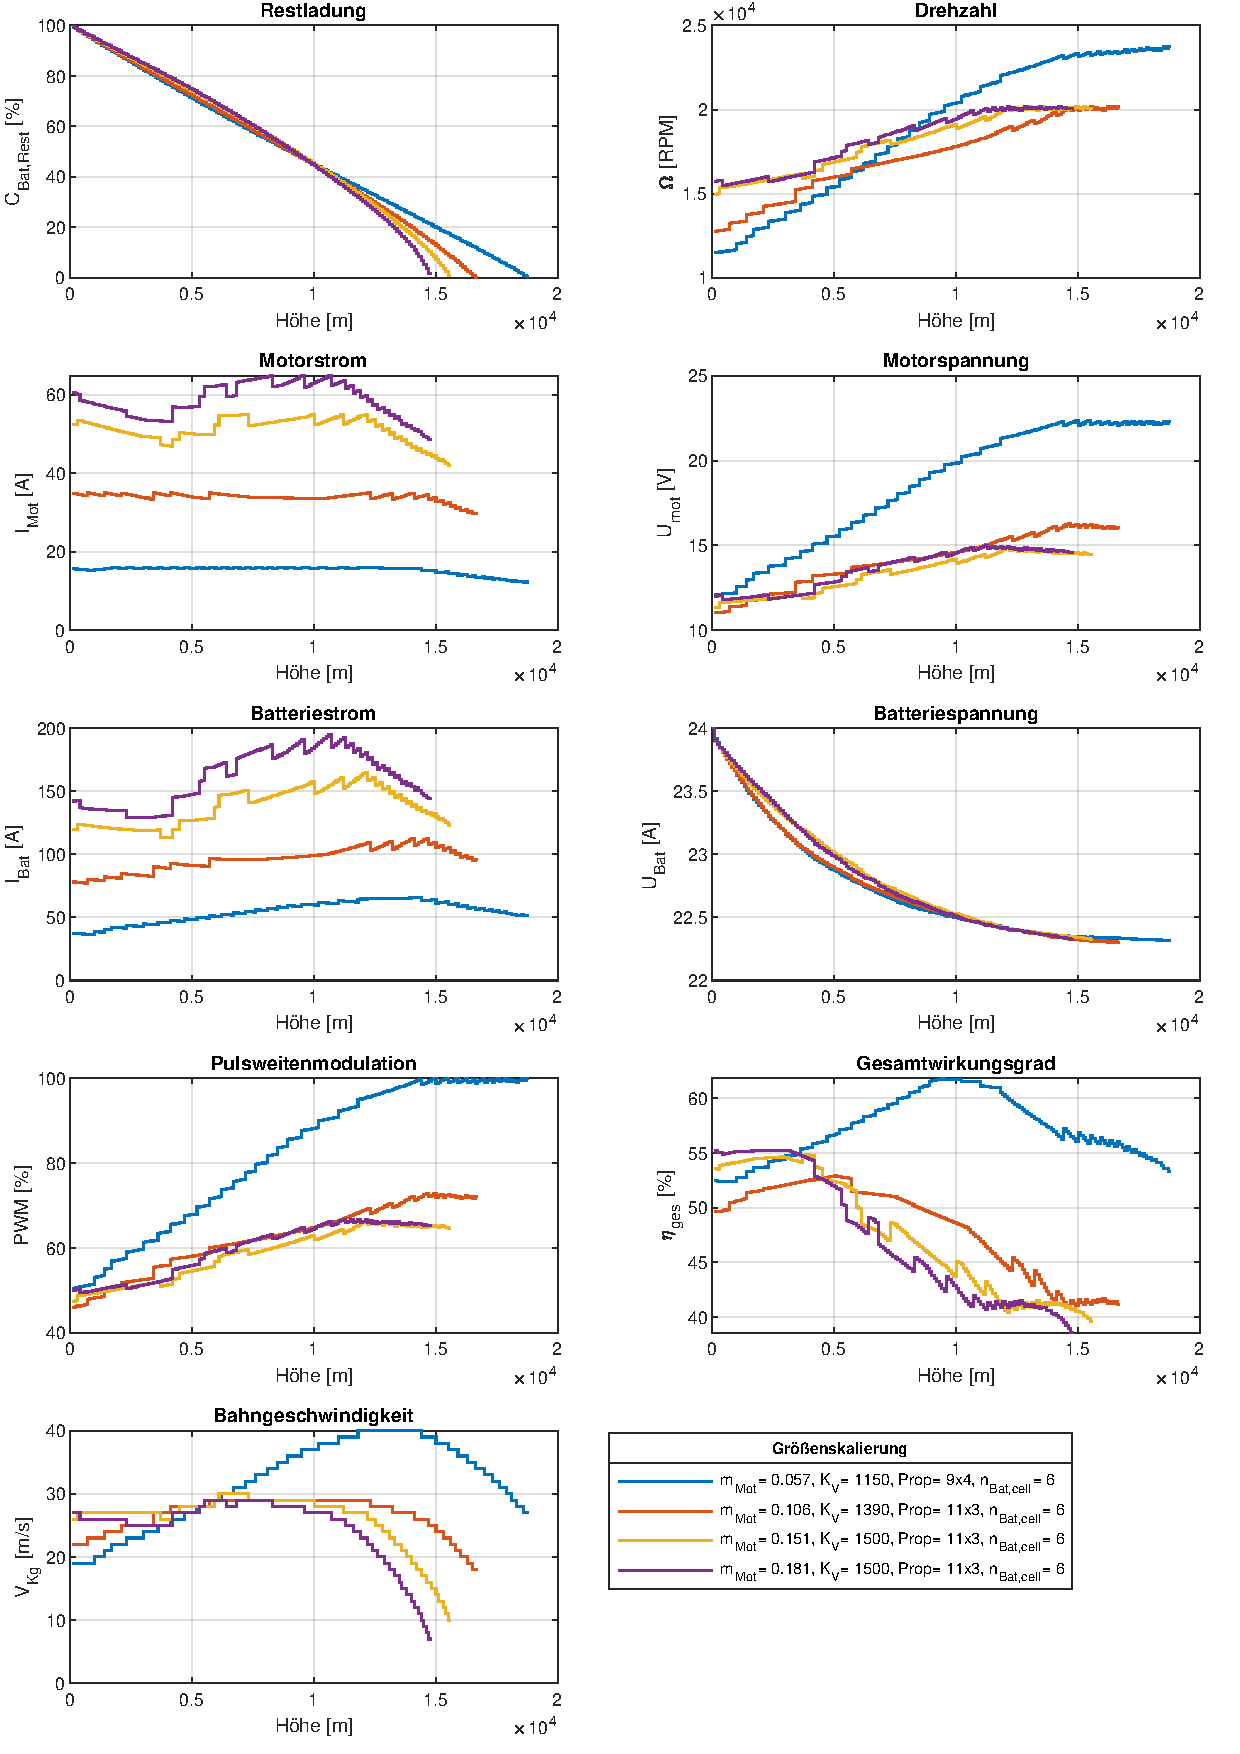
\includegraphics[scale=0.7]{Diagramme/Groessenskalierung.pdf}
	\caption{Einfluss der Größenveränderung auf die maximal erreichbare Höhe}
	\label{abb:groessenskalierung}
\end{figure}
Eine äquivalente Größenskalierung besitzt einen vernachlässigbar kleinen Einfluss auf die Kostenfunktion, die maximale Höhe (Vgl. Abb. \ref{abb:groessenskalierung}). Der Grund für die Unterschiede in den Diagrammen liegt in den Unterschieden der Motoren und Propeller. Eine hundertprozentig uniforme Skalierung ist hier nicht möglich. Dabei unterscheiden sich besonders die \ensuremath{K_V}-Werte der Motoren. Dies zieht Unterschiede im Bereich der Motorspannung und folglich in der PWM und im Gesamtwirkungsgrad nach sich.
\textcolor{red}{Dies wird weiterhin begründet durch Begründung für Reichweitenunabhängigkeit von der Flugmasse}. An dieser Stelle kann somit festgehalten werden, dass eine Größenskalierung keinen Einfluss auf die Flugleistungen hat. Die Vorteile eine größeren Masse liegen für reale Anwendungsfälle vorrangig in der Massenträgheit. In einem Höhensektor von \SI{0}{} bis \SI{15000}{m} treten im Durchschnitt \SI{100}{km/h} starke Winde auf. 
\todo[inline]{Quelle für Höhenprofil, Falk}
Die Einflüsse von Böen in diesen Größenordnungen auf einen Multicopter fällt geringer aus, wenn die Masse höher. Dies erfordert im Umkehrschluss weniger Energie zur Kurs- und Lagekorrektur.


\subsection{Anzahl der Propeller}
Wie sich oben zeigte, hat eine uniforme Skalierung des Fluggerätes keinen Einfluss auf dessen Flugleistung. Bisher wurde dabei nur Fluggeräte mit vier Rotoren untersucht. Dabei gilt es noch die Abhängigkeit der Flugleistungen von der Rotoranzahl zu überprüfen. 

\subsection{Ergebnisse}
\begin{figure}[H]
%\centering
	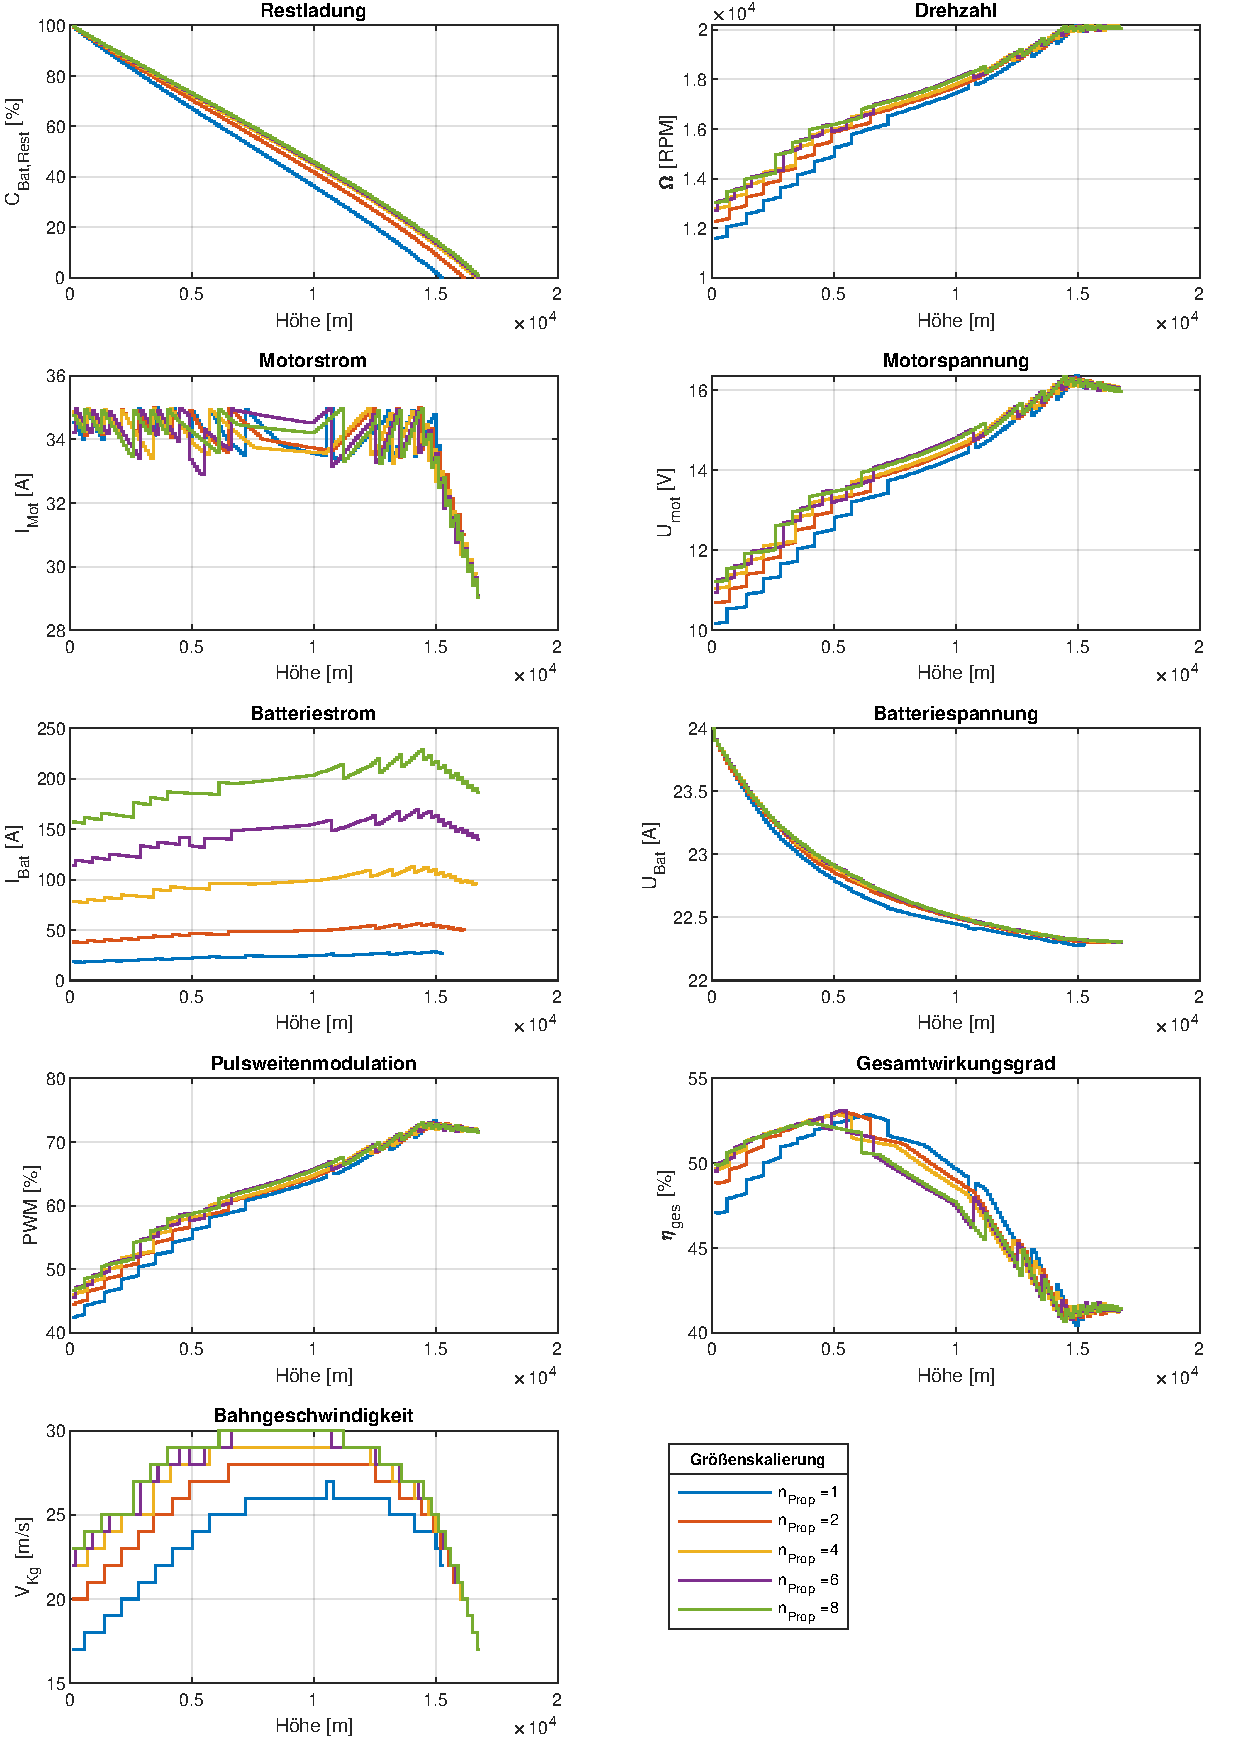
\includegraphics[scale=0.7]{Diagramme/Anz_Prop.pdf}
	\caption{Einfluss der Propelleranzahl auf die maximal erreichbare Höhe (\ensuremath{m_{Mot}=\SI{106}{g}}, \ensuremath{K_V=\SI{1390}{RPM/V}}, \ensuremath{n_{Prop}=4}, \ensuremath{Propeller=\SI{10x3}{}}, \ensuremath{n_{Bat,cell}=4}, \ensuremath{u_{Wg}=\SI{10}{m/s}})}
	\label{abb:groessenskalierung}
\end{figure}
Analog zu den obigen Ergebnissen bewirkt eine äquivalente Veränderung der Rotoranzahl keine nennenswerten Änderungen der maximalen Flughöhe für gleiche Motoren. Die Begründung ist dieselbe wie Kapitel \ref{subsec:ergebnisse_groesse}. Die Ergebnisse für einen Multicopter mit vier, sechs oder acht Propellern sind nahezu identisch. Dies gilt auch für die Restladung, die für diese Konstellationen noch am größten ausfällt. In Bezug auf Abschn. \ref{subsec:ergebnis_massenverteilung} sind diese den Konstellationen mit weniger Rotoren vorzuziehen. \\
An dieser Stelle sind jedoch Einschränkungen vorzunehmen. 
Der Monocopter erreicht die gleiche maximale Höhe wie die anderen Konstellationen. Der Monocopter benötigt jedoch zusätzlich noch Aktuatorik für die Abdeckung aller vier Stellgrößen. Dies sind die 3 rotatorischen (Rollen, Nicken und Gieren) und eine translatorische Stellgröße. Weiterhin muss ein Drehmomentenausgleich vollzogen werden, sei es durch einen Heckrotor, eine angepasste Steuerung, die Formgebung des Rumpfes oder durch sonstige Mechanismen. Diese zusätzliche Aktuatorik benötigt der Duocopter ebenfalls. Ein Drehmomentenausgleich ist hier jedoch nicht notwendig.
Beide erwähnten Punkte erhöhen die Gesamtmasse und benötigen zusätzlich Energie. Dies verringert die Gesamthöhe. 
Für mehr als vier Propeller muss berücksichtigt werden, dass die Gesamtmasse und damit insbesondere das Strukturgewicht steigt. Dies geht auf die Kosten einer optimalen Konstellation der Massenverteilung. Zusätzlich erhöht sich die obere Stirnfläche \ensuremath{A_{copter,oben}} durch stärkere Strukturen, die in einer Widerstandserhöhung und somit erhöhten Verlusten resultieren. Um das oben gesagte zusammenzufassen, eignet sich eine Propelleranzahl von vier am besten für einen Flug in die untere Strathosphäre. 



\section{Verstellpropeller}
\label{sec:verstellprop}
Ein bisherige Begrenzung der Flugleistungen erfolgte häufig durch die maximale Drehzahl des Propellers, die indirekt die Motorspannung beeinflusst. 
Besonders auffällig bei vorherigen Untersuchungen (vor allem in Bezug auf die Untersuchungen des Quadrocopters aus Kap. \ref{chap:nachbildung}) ist, dass bei Propeller mit einer geringen Steigung die Drehzahl deutlich schneller steigt, als bei einem Propeller mit einer großen Steigung. Da vor allem die Drehzahl die Motorspannung bestimmt, ist eine Verringerung der Drehzahl bei gleichem Schub von Interesse. Mit zunehmender Flughöhe verringert sich die Dichte und damit auch der Schub, wenn die Rotordrehzahl oder die Propellersteigung konstant gehalten werden. Diesem kann mit einer Erhöhung der Drehzahl oder mit einer Erhöhung der Steigung ausgeglichen werden. Während bei einem Drehflügler mit Strahltriebwerk nur eine Blattverstellung, nicht aber eine Drehzahlerveränderung möglich ist, besitzen elektrisch, propellergetriebene Fluggeräte beide Möglichkeiten. Dies kann mit einem Verstellpropeller und entsprechender Aktuatorik realisiert werden. \\
Im Rahmen dieser Untersuchung liegen nur Propellerkennfelder mit einer konstanten Propellersteigung vor. Das Vorgehen für einen Propeller mit variabler Steigung sieht so aus, dass für einen vorgegebenen Durchmesser alle Kennfelder mit diesem Durchmesser der Datenbank entnommen werden. Danach wird in der Leistungsuntersuchung jeder Propeller mit unterschiedlicher Steigung, aber gleichem Durchmesser, gegeinander abgewogen. Die Auswahl für den in dem betrachteten Flugmoment beste Steigung erfolgt wieder über die Energiebetrachtung, analog zum Bahnneigungswinkel und der Bahngeschwindigkeit.


\subsection{Ergebnisse}
\begin{figure}[H]
%\centering
	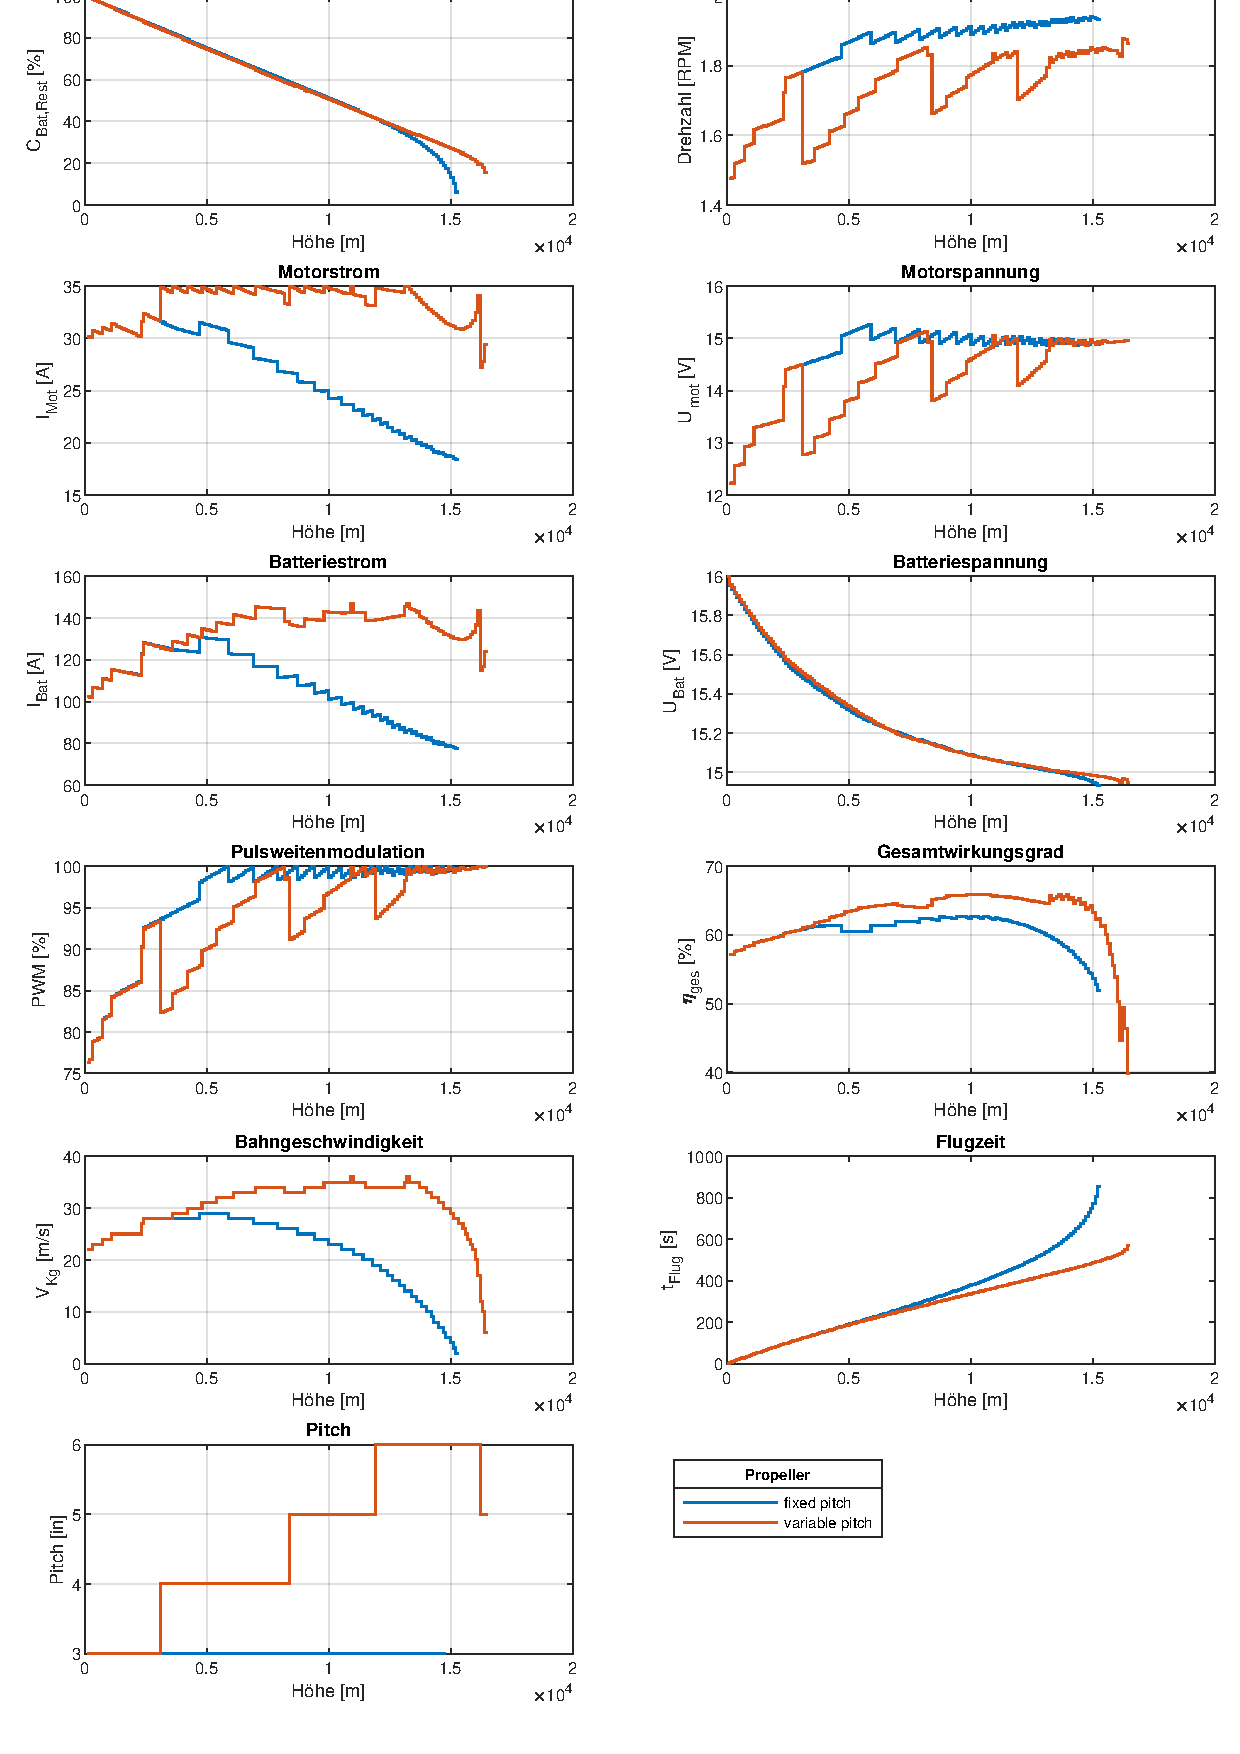
\includegraphics[scale=0.7]{Diagramme/Verstellpropeller.pdf}
	\caption{Verstellpropeller}
	\label{abb:verstellpropeller}
\end{figure}
Der zusätzliche Höhengewinn durch einen Verstellpropeller ist gerade einmal \SI{1000}{m}. Die Leistungsparameter beider Propellerarten sind für die ersten \SI{3000}{m} identisch. Dies liegt an der gleichen Propellersteigung. Zuerst ist wieder ein Flug mit maximalen Motorstrom am effizientesten bis die PWM wieder \SI{100}{\%} erreicht und folglich der Motorstrom und der Batteriestrom abfallen. Da die Motorspannung konstant bleibt, bleibt auch die Drehzahl konstant. Die Bahngeschwindigkeit sinkt jedoch kontinuierlich ab. Während sich dieser Zustand beim Propeller mit fester Propellersteigung nicht ändert, ist ab \SI{10000}{m} Steigflug ein Anstellwinkel von \SI{4}{in} für den Verstellpropeller energetisch effizienter. Dies bewirkt, dass die Drehzahl und damit einhergehend die Motorspannung abfällt, während gleichzeitig der Motorstrom zum zweiten Mal auf sein maximales Niveau steigt. Gleichzeitig steigen auch der Wirkungsgrad und die Bahngeschwindigkeit erneut. Dieser Zustand kann ebenfalls wieder solange gehalten werden bis die PWM \SI{100}{\%} erreicht und somit die Bahngeschwindigkeit bis auf \SI{0}{m/s} absinkt. Damit ist das Ende des Steigflugs erreicht. \\





	Der Vorteil eines Verstellpropellers ist vergleichsweise gering. Dazu müssen auch noch folgende Einschränkungen vorgenommen werden. Der Verstellpropeller kann nur im Rahmen der in der APC-Datenbank vorhanden Propeller modelliert werden. Dies setzt Ungenauigkeiten voraus, da eine kontinuierliche Verstellung nicht nachgebildet werden kann und nur so viele Verstellungen berücksichtigt werden können, wie auch Propeller mit verschiedenen Steigungen in der Datenbank vorhanden sind. \textcolor{red}{Zudem ist man auf die Kennfelder angewiesen.}. An dieser Stelle wurde der Propeller in gewisser Weise idealisiert. So wurde unter anderem die verlängerte Blattaufhängung außer Acht gelassen. Dies führt zu zusätzlichen Verlusten an der Blattwurzel und einer Verringerung des effektiven Radius. Bei einem Propeller mit konstantem Anstellwinkel kann diese sehr kurz gehalten werden, weshalb das profilierte Rotorblatt deutlich früher beginnt. Dies ist bei dem hier modellierten Verstellpropeller nicht berücksichtigt worden.\\
Weiterhin wurden in dieser Betrachtung das Gewicht des Verstellmechanismus an sich und der Aktuatorik für jeden einzelnen Propeller nicht berücksichtigt. Weiterhin bedeuten die Aktuatoren zusätzliche Verbraucher, die mitunter deutlich schneller zu einem Flug bei \SI{100}{\%} PWM führen würden. Letztendlich ist der fehlende Schub in großen Höhen nicht das Begrenzungsmerkmal, sondern die Drehzahl des Propellers und Motors sowie die Batteriespannung. Letztere macht den Verstellpropeller ein weiteres Stück redundant (Vgl. \textcolor{red}{Anhang}). Mit einem hohen Batteriestrom verschiebt sich der Bereich, in dem ein größere Steigung vorteilhafter ist, noch weiter in größere Höhen. Damit sinkt auch die Einsatzdauer und schließlich der Nutzen. 
Schlussendlich bringt der Verstellpropeller den Vorteil der Autorotation mit, der weniger für den Steigflug als für den anschließenden Sinkflug von Bedeutung ist. Durch die Autorotation ist ein antriebsloser Sinkflug möglich. Damit könnte die Batterie noch weiter entladen werden bevor ein Sinkflug eingeleitet werden muss, was im Umkehrschluss die erreichbare Höhe steigert. 

%\begin{itemize}
%	\item Der Verstellpropeller bringt gerade einmal einen Vorteil von \SI{1000}{m}Höhe.
%	\item Die Leistungsparameter sind für die ersten \SI{10000}{m} identisch. Dies liegt am gleichen Pitch.
%	\item Zuerst ist wieder ein Flug mit maximalen Motorstrom am effizientesten bis die PWM wieder \SI{100}{\%} erreicht und folglich der Motorstrom und der Batteriestrom abfallen. Da die Motorspannung konstant bleibt, bleibt auch die Drehzahl konstant. Die Bahngeschwindigkeit sinkt jedoch kontinuierlich ab.
%	\item Während sich beim fixed pitch Propeller dieser Zustand nicht ändert, kann der variable pitch Propeller der
%	\item ab \SI{10000}{m} ist ein Steigflug mit einem Pitch von \SI{4}{in} effizienter. 
%	\item Dies bewirkt, dass die Drehzahl und damit einhergehend die Motorspannung abfällt, während gleichzeitig der Motorstrom zum zweiten Mal auf sein maximales Niveau steigt. Gleichzeitig steigen auch der Wirkungsgrad und die Bahngeschwindigkeit erneut. Dieser Zustand kann ebenfalls wieder solange gehalten werden bis die PWM \SI{100}{\%} erreicht und somit die Bahngeschwindigkeit bis auf \SI{0}{m/s} absinkt. Damit ist das Ende des Steigflugs erreicht. \\
%	Der Vorteil eines Verstellpropellers ist vergleichsweise gering. Dazu müssen auch noch folgende Einschränkungen vorgenommen werden. Der Verstellpropeller kann nur im Rahmen der in der APC-Datenbank vorhanden Propeller modelliert werden. Dies setzt Ungenauigkeiten voraus, da eine kontinuierliche Verstellung nicht nachgebildet werden kann und nur so viele Verstellungen berücksichtigt werden können, wie auch Propeller mit verschiedenen Pitches in der Datenbank vorhanden sind. \textcolor{red}{Zudem ist man auf die Kennfelder angewiesen.}. An dieser Stelle wurde der Propeller in gewisser Weise idealisiert. So wurde unter anderem die verlängerte Blattaufhängung außer Acht gelassen. Dies führt zu zusätzlichen Verlusten an der Blattwurzel. Bei einem Propeller mit konstantem Anstellwinkel kann diese sehr kurz gehalten werden, weshalb das effektive Blatt bei einem deutlich kleineren Radius anfängt.
	
%Unter anderem wurden in dieser Betrachtung das Gewicht des Verstellmechanismus an sich und der Aktuatorik für jeden einzelnen Propeller nicht berücksichtigt. Weiterhin bedeuten die Aktuatoren zusätzliche Verbraucher, die mitunter deutlich schneller zu einem Flug bei \SI{100}{\%} PWM führen würden. Letztendlich ist der fehlende Schub in großen Höhen nicht das Begrenzungsmerkmal, sondern die Drehzahl des Propellers und Motors sowie die Batteriespannung. Letztere macht den Verstellpropeller ein weiteres Stück redundant (Vgl. \textcolor{red}{Anhang}). Mit einem hohen Batteriestrom verschiebt sich der Bereich, in dem ein größerer Pitch vorteilhafter ist, noch weiter in größere Höhen. Damit sinkt auch die Einsatzdauer und schließlich der Nutzen. 
%Schlussendlich bringt der Verstellpropeller einen entscheidenden Vorteil der Autorotation mit, der weniger für den Steigflug als für den anschließenden Sinkflug von Bedeutung ist. Durch die Autorotation ist ein antriebsloser Sinkflug möglich. Damit könnte die Batterie noch weiter entladen werden bevor ein Sinkflug eingeleitet werden muss, was im Umkehrschluss die erreichbare Höhe steigert. 
%	\item somit ergibt sich keinerlei Vorteil für die Benutzung eines Verstellpropellers
%	\item Trotzdem muss berücksichtigt werden, das der Propeller nur im Rahmen der in der APC-Datenbank vorhanden Propeller modelliert werden kann.
%	\item dies setzt Ungenauigkeiten voraus, da eine kontinuierliche Verstellung nicht nachgebildet werden kann und nur so viele Verstellungen berücksichtigt werden können, wie auch in der Datenbank vorhanden sind
%	\item außerdem ist man auf die Kennfelder angewiesen
%	\item kann aber für den Sinkflug bedeutend sein, weil mit der Verstellung die Autorotation ermöglicht wird
%\end{itemize}


\section{Stufenloses Getriebe}
\label{sec:getriebe}
Eine häufige Begrenzung der Leistung ist die maximale Drehzahl des Motors oder des Propellers. Diese nimmt mit großen Höhen stark zu. Ein stufenlos verstellbares Getriebe bringt Vorteile in der Begrenzung der maximalen Drehzahl (Machzahleffekte, Strömungsablösung etc.), dass heißt durch den Einsatz eines Getriebes kann die Drehzahl für den Motor entsprechend angepasst werden, sodass diese nicht mehr den Flaschenhals für einen Steigflug darstellt.
Die Übersetzung für ein Getriebe 
\begin{equation}
	i = \frac{\omega_{an}}{\omega_{ab}} 
	\label{eq:getriebe_uebersetzung}
\end{equation}
setzt sich in Abhängigkeit der Drehzahlen aus dem Verhältnis der Eingangsdrehzahl \ensuremath{\omega_{an}} zur Ausgangsdrehzahl \ensuremath{\omega_{ab}} zusammen. Weiterhin gilt für die Leistung, dass unter Berücksichtigung von Verlusten innerhalb des Getriebes die Eingangsleistung \ensuremath{P_{an}} gleich der Ausgangsleistung \ensuremath{P_{ab}} ist
\begin{equation}
	P_{an} = \eta_{Getriebe} \cdot \omega_{an}\cdot M_{an} = \omega_{ab}\cdot M_{ab} = P_{ab}
	\label{eq:getriebe_leistung}
\end{equation} 
mit dem Wirkungsgrad 
\begin{equation}
	\eta_{Getriebe} = \frac{P_{ab}}{P_{an}} \leq 1.
	\label{eq:getriebe_wirkungsgrad}
\end{equation}
Aus den Gleichungen \ref{eq:getriebe_uebersetzung} bis \ref{eq:getriebe_wirkungsgrad} ergeben sich nun für die aus dem Propellerkennfeld ermittelten Drehzahl und dem Drehmoment die neue Drehzahl für den Motor
\begin{equation}
	\omega_{neu} = \omega_{Kennfeld}\cdot i
\end{equation}
und aus der Leistung
\begin{equation}
	M_{neu} = \frac{P_{ab}}{\omega_{neu}}.
\end{equation}
das neue Drehmoment.
Die günstigste Übersetzung wird analog zum Steigwinkel des Flächenflugzeuges und analog zur Steiggeschwindigkeit durch eine Iteration über der Übersetzung \ensuremath{i} gefunden. Das Entscheidungskriterium ist auch hier die minimal aufgebrachte Energiemenge für den jeweiligen Höhenschritt. An dieser Stelle ist das Getriebegewicht \texttt{m\_Getriebe} nicht zu vernachlässigen. Diese fließt mit der Anzahl der Propeller in die Berechnung der Gesamtmasse mit ein
\begin{equation}
	m = m_{Bat} + (m_{Mot} + m_{Getriebe})\cdot n_{Prop} + m_{Copter} .
\end{equation}


\textcolor{red}{hier noch untersuchen, wie sich die KV Wert auf die Leistung auswirkt bei gleichem Motorgewicht. Außerdem noch feststellen, in welche Richtung die Drehzahl gewandelt wird}

\begin{itemize}
	\item KV Wert beeinflusst Übersetzung
\end{itemize}

\subsection{Ergebnis}
Der Einsatz eines idealen, stufenlosen Getriebes (\ensuremath{m_{Getriebe} = 0} und \ensuremath{\eta_{Getriebe} = 1}) erzeugt einen erheblichen Höhengewinn. Für die gewählte Konstellation bedeutet dies einen TOC von ca. \SI{17000}{m}. Das ist ein Zuwachs von mindestens \SI{2000}{m} zum Multicopter ohne Getriebe. Das CVT (continuously variable transmission)-Getriebe übersetzt dabei die Drehzahl des Motors, das heißt die Propellerdrehzahl ist größer als die des Motors. \\
Zu Beginn des Fluges übersetzt das Getriebe die Motordrehzahl mit einer Übersetzung von \SI{1,4}{} ins Langsame. die Drehzahl des Propellers beträgt dabei \SI{20000}{U/min}. Es folgt eine hyperbolische Abnahme der Übersetzung durch das Getriebe und damit auch der Drehzahl. Der Motor wird bei maximaler Last betrieben, das heißt beim maximalen Motorstrom von \SI{25}{A} und bei Volllast (PWM =  \SI{100}{\%}). Die PWM schwankt in einem Bereich von \SI{5}{\%} in der Nähe von \SI{100}{\%}. Die Sprünge, die im Verlauf der Drehzahl, Des Motorstroms und der PWM zu verzeichnen sind, können auf die gewählte Diskretisierung der Getriebeübersetzung zurückgeführt werden. \textcolor{red}{Das stufenlose Getriebe ermöglicht den optimalen Betrieb des Motors, welcher in diesem Fall bei voller Leistungsentnahme ist. Es ermöglicht eine derartige Wandlung des der Drehzahl, sodass einerseits die PWM bei \SI{100}{\%} ist und andererseits der Motorstrom dem maximalen Dauerstrom entspricht. Also ein Betriebspunkt bei Volllast. Dies kann durch das Getriebe dauerhaft gehalten werden.} 
Die Steiggeschwindigkeit weist einen beinahe asymptotischen Verlauf von anfänglich \SI{21}{m/s} an den Grenzwert von \SI{26}{m/s} auf. Entsprechend dieser hohe Geschwindigkeiten braucht der Quadrocopter nur \SI{14}{min} und \SI{9}{s} bis zum Erreichen der maximalen Höhe.

In der Realität besitzt ein stufenloses Getriebe jedoch immer ein Eigengewicht und zeichnet sich durch einen vergleichsweise schlechten Wirkungsgrad aus (\SI{0.8}{} zu etwa \SI{0.95}{} bei einem Stufengetriebe).
\todo[inline]{Quelle} Die hohen Verluste liegen in der hohen erforderlichen Reibkraft und Verstellkraft begründet. Unter Berücksichtigung dieser verringert sich der Höhengewinn schrittweise, je größer das Getriebegewicht und dessen Verluste ausfallen. Stufenlose Getriebe existieren im Modellbau, allerdings nur für Lastkraftwagenmodelle. Das Gewicht eines einzelnen Getriebes beläuft sich dabei auf mehr als \SI{700}{g}, wobei die Verstellelektronik nicht berücksichtigt wurde. Für einen vierrotorigen Multicopter entspräche das einem Zusatzgewicht von mehr als \SI{2800}{g}. 
Trotz seines Nutzens für die Höhenleistung werden die Vorteile eines CVT-Getriebes durch dessen Nachteile überkompensiert. Ein solches Getriebe bedeutet bei all seiner Kampaktheit und Effizienz letztendlich große Zusatzmasse und einen weitere, verlustbehaftete Komponenten innerhalb der Antriebskette. In Bezug auf die optimale Massenverteilung aus Kapitel \ref{sec:massenverteilung} und die besagte Richtung einer Optimierung der Verhältnisse verändert Getriebe die Massenaufteilung in Richtung einer schlechteren. Aus all diesen Gründen kann von dem Einsatz eines CVT-Getriebes abgesehen werden.



\section{Randbedingungen des Aeromot\_UAV-Projekts}
\begin{itemize}
	\item Schlussendlich soll noch unabhängig von den vorherigen Ergebnissen der Einfluss der für dieses Projekt bestimmten Randbedingungen festgehalten werden
	\item diese betragen 
	\item 
	\begin{center}
	\captionof{table}{wichtige Parameter des Flächenflugzeugs}
	\begin{tabular}{l l l} \hline
		Parameter & Variablenname & Wert \\ \hline
		Windgeschwindigkeit \ensuremath{u_{Wg}} & \texttt{u\_Wg} & \SI{100}{km/h}\\
		Nutzlast \ensuremath{m_{Nutz}} & \texttt{m\_Nutz} & \SI{250}{g}  \\ \hline
	\end{tabular}	
	\label{tab:flzg_parameter}
\end{center}
\end{itemize}
    \chapter{Zusammenfassung und Ausblick}

\section{Zusammenfassung}
Zusammengenommen gibt es viele Einflüsse auf das Flugleistungsverhalten von elektrisch, propellergetriebenen Fluggeräten. 
Im Rahmen der Genauigkeit des Programms erweist sich ein Multicopter als geeigneter für einen Steigflug auf \SI{10000}{m} oder sogar \SI{15000}{m} Höhe. In diesem Zusammenhang sollte das Flächenflugzeug nicht vernachlässigt werden. Wie in Abschn. \ref{subsubsec:anz_mot_flaechenflzg} beschrieben wurde, ist der günstigste Flugzustand für ein Flächenflugzeug mit mehr als einem Motor der Vertikalflug. Dies legt die Verwendung eines VTOL-Fluggerätes nahe. Ein derartiges Fluggerät verbindet die Vorteile eines Multicopters, die da wären: Senkrechtstarterfähigkeiten (und Landung)und kleine Abmaße, mit denen des Flächenflugzeugs, was hauptsächlich den antriebslosen Gleitflug beinhaltet. Ein möglicher Flug sähe dann den vertikalen Steigflug bis zum Erreichen der vorgesehenen Dienstgipfelhöhe vor und einen anschließenden Sinklug im Gleiten. \\
Ein sehr großen Einfluss auf die Flugleistungen hat die Motor-Propeller-Kombination (Kap. \ref{subsubsec:mot_prop_kombi}. Prinzipiell ist ein Motor mit hohem \ensuremath{K_V}-Wert zu verwenden, der zusätzlich mit einen hohen, dauerhaften Motorstrom belastet werden kann. Der Propeller ist in Bezug auf den Motor anzupassen. \\
Die Verlustleistungen kann durch eine aerodynamisch günstige Verkleidung aller Fluggeräteinheiten minimiert werden (Kap. \ref{subsec:widerstandseinfluss}. Dies würde auch die Verstellvorrichtungen für einen Verstellpropeller oder ein Getriebe betreffen. Den mitunter signifikantesten auf die erreichbare Höhe hat die Wahl der Batterie (Kap. \ref{subsec:einfluss_n_bat} sowie \ref{sec:massenverteilung}). Als ertes sollte diese eine hohe Kapazität besitzen, da dies häufig das Kriterium für erreichbare Höhe darstellt. Weiterhin ist eine hohe Batteriespannung durch die Batteriezellenanzahl zu erreichen. Dies ist jedoch mit Rücksicht auf den Motor und mit Bedacht zu wählen, da eine hohe Batteriespannung eine Reduktion der Kapazität bewirkt (Kap. \ref{subsec:einfluss_n_bat}). Auch die Batteriemasse hat Einfluss auf die Flugleistungen. Ein Verhältnis zwischen \SI{50}{\%} und \SI{60}{\%} liefert die besten Ergebnisse (Kap. \ref{sec:massenverteilung}). Die Anzahl der Propeller oder die Größe hat bei einer äquivalenten Skalierung des Systems weiterhin einen vernachlässigbar kleinen Einfluss auf die Kostenfunktion (Kap. \ref{sec:groesse}. \\
Es stellte sich heraus, dass vor allem die maximale Motordrehzahl durch die Batteriespannung die Drehzahl des Propellers und damit die Höhe begrenzt. Ein Verstellpropeller (Kap. \ref{sec:verstellprop}) erzielt einen zusätzlichen Höhengewinn. Dies ist aber nur der Fall, wenn der Verstellmechanismus und die Aktuatorik kein zusätzliches Gewicht besitzen. Das gleiche gilt für ein Getriebe. Auch hier sind nur Höhengewinne zu erreichen, wenn das Getriebe als ideal betrachtet wird, d.h. kein Eigengewicht u. keine Verluste. Dies ergibt zusammengenommen, dass sich der Einbau eines Vertellpropellers oder eines Getriebes nicht lohnt. Für größere und schwerere Multicopter fällt das Eigengewicht nicht so sehr ins Gewicht. 


\todo[inline]{morgen nochmal überarbeiten}


%In Bezug auf die Ergebnisse sind auch viele Einschränkungen vorzunehmen

%\begin{itemize}
%	\item viele Werte für den Multicopter sind reine Schätzwerte und bedürfen einer Validierung durch Messungen und Testflügen
%	\item insgesamt beinhaltet das Programm viele einfach Modelle, so z.B. das des Motors, die viele Effekte nicht berücksichtigen
%	\item dies umfasst die Strahltheorie, das Motormodell, den Regler
%	\item beim Motor werden die Verlustgrößen (\ensuremath{R_i} und \ensuremath{I_0}) als konstant angenommen und kein Einfluss der Temperatur berücksichtigt.
%	\item dies gilt auch für das Batteriemodell, auch hier keine Berücksichtigung von Temperatureinflüssen, die bei den hier angesetzten Flughöhen definitiv zu erwarten sind 
%	\item das Modell des Flächenflugzeuges ist sehr einfach gewählt und berücksichtigt nicht die realen Gegebenheiten
%	\item es wurden viele grenzen innerhalb der flugenvelloppe vernachlässigt, die mit dem einfachen Modell nicht behandelt werden können. Das sind die Auftriebsgrenze, die Festigkeitsgrenze und die Wärme u. Temperaturgrenze. Vor allem die Auftriebsgrenze kann noch eine wichtige Rolle spielen. 
%	\item Durch die oben genannten Eigenschaften des Flächenflugzeugmodells sind auch viele Widerstände vorhanden, die nicht in das Modell mit einfließen. Diese können nur durch exakte Kenntnis der aerodynamischen Gegebenheiten, welche in Flugversuchen ermittelt werden können wie dies in \cite{Ostler.2006} der fall ist, berechnet werden (Nullwiderstand, Wellenwiderstand, etc.)
%	\item diese können nur drch Kenntnis über das Flügelprofil bestimmt werden
%	\item Es ist ein sehr einfaches Luftmodell verwendet worden, dass Reynolds oder Machzahleffekte nicht berücksichtigt. 
%	\item das sind unter anderem Einstellungen, die den Throttle betreffen (Abriegelung nach oben, um das Fluggerät handbar zu halten, oder der Modus position hold, der zur Positionshaltung wieder zusätzlich Energie benötigt)
%	\item insgesamt handelt es sich hier auch um ein statisches Modell, dynamische Effekt bleiben hierbei unberücksichtigt, z.b. Ausgleich durch Böen
%	\item Optimierungen in Richtung einer Rechenleistungserhöhung können durch die Verwendung alternativer Algorithmen (z.B. divide and conquer) erzielt werden, anstatt der hier verwendeten Brute Force Methode.
%%	\item insgs sind sehr positive Grundvoraussetzungen getroffen worden, die die Umgebungsparameter betreffen. Die Winde wurden mit einer konstanten Windgeschwindigkeit von \SI{10}{m/s} mit einbezogen. Dies ist für einen Multicopter vom Vorteil, weil es einem langsamen Vorwärtsflug gleichkommt, der den Leistungsüberschuss erhöht. Durch den Vorwärtsflug wird die induzierte Leistung verringert \cite[S.329]{Wall.2015}. Schlechtere Ergebnisse sind mit größeren oder geringeren Windgeschwindigkeiten zu erwarten.
%	\item mit den im AEROMET UAV angenommenen Umgebungsbedingungen, die eine zusätzliche Nutzlast und sehr hohe, wechselnde Windstärken annehmen, liegen die zu erwartenden Leistungen nochmal um \SI{1000}{\%} unter den hier errechneten. 
	
%	\item es zeigt sich, dass es viele verschiedene Ansatzpunkte für die Optimierung eines Fluggerätes zum effizienten Aufstieg in die untere Stratosphäre gibt. 
%	\item für diese Mission erweist sich ein Multicopter als effizienter und mit Berücksichtigung der Rahmenbedingungen einfacher zu händeln. 
%	\item hier sei wieder auf das einfache Modell des Flächenlfugzeugs verwiesen
%	\item Die Gestaltung des Copters sollte mglst. aerodynamisch sein, eine große Batterie besitzen.
%	\item Alle Komponenten sollten gut aufeinander abgestimmt sein, das betrifft vor allem die Batteriemassenverteilung, die Anzahl der Propeller
%	\item für einen Multicopter ergibt sich eine optimale Anzahl von vier Rotoren.
%	\item Bei ebendiesem Fluggerät würde sich der Einbau eines Getriebes auszahlen, wenn dieses effizient und leicht gestaltet ist.
%	\item für einen reinen Quadrocopter werden die Vorteile von einem getriebe oder einem Verstellpropeller durch dessen Nachteile überkompensiert, sodass sich Einsatz nicht auszahlt sondern eher die Flugleistungen verschlechtert. Deshalb ist umso mehr auf die vorangegangenen Punkte zu achten
%	\item der Quadrocopter aus \cite{Anderson.2018} kann als die Richtung des Designs aufgefasst werden, die für die Konstruktion eines Multicopters die besten Ergebnisse liefert.
%\end{itemize}


\section{Ausblick}
Der nächste Schritt ist die Validierung der in dieser aufgestellten Arbeit. Dies sollte möglichst in praktischen Versuchen geschehen wie dies in \cite{Ostler.2007},\cite{PCUP}. Mit der fortschreitenden Entwicklung von Batterien steigt auch die Leistungsfähigkeit und die Reichweite der UAVs. Das immer größer werdende Anwendungsfeld der unbemannten Flugeräte steigt zusätzlich, was die Weiterentwicklung nochmals beschleunigt.
Die UAVs stellen eine gute Alternative zu den Wetterballonen dar. Auch wenn sie nicht ganz über die Höhe verfügen wie sie Wetterballone erreichen. Nichtsdestotrotz stellen sie eine sichere und wiederverwendbare Lösung dar.

\begin{itemize}
	\item nächster Schritt ist die validierung der Ergebnisse in Flugversuchen und Flugmessungen. 
	\item bei der bisherigen Optimierung wurden nur einzelne Parameter ausgewählt und diese Optimiert. 
	\item an dieser Stelle fehlt eine globale Optimierung, die alle Variationen aller Parameter durchrechnet und und dann das bester Ergebnis resultiert. 
	\item dies erhöht die Genauigkeit der Untersuchung von Abhängigkeiten.
	\item Ein Modell hierzu wird z.B. in \cite{Magnussen.2015} vorgeschlagen
	\item zusätzlich ist einer Verfeinerung der Modelle anzustreben. Dies betrifft insbesondere das Flächenflugzeugmodell.
	\item Für alle untersuchungen wären Datenbanken und Modelle angemessen, die eine Abhängigkeit von der masse aufweisen.
\end{itemize}
    %\chapter{Projektmanagement}
\label{projektmanagement}

%%%%%%%%%%%%%%%%%%%%%%%%%%%%%%%%%%%%%%%%%%%WBS%%%%%%%%%%%%%%%%%%%%%%%%%%%%%%%%%%%%%%%%%%%%

\begin{landscape}
\section{Projektstrukturplan}
% 	\captionof{Projektstrukturplan}
\label{WBS}
        \vspace{0.5cm}
        \begin{tikzpicture}[node distance=0.7cm]
            \tikzstyle{abstract}=[rectangle, draw=black, rounded corners, fill=blue!50, drop shadow,
        text centered, anchor=north, text=white, text width=3.5cm]
    \tikzstyle{topabstract}=[rectangle, draw=black, rounded corners, fill=blue!20, drop shadow,
        text centered, anchor=north, text width=0.8\linewidth]
    \tikzstyle{subabstract}=[rectangle, draw=black, rounded corners, fill=blue!20, drop shadow,
        text centered, anchor=north, text width=3.5cm]
    \tikzstyle{myarrow}=[->, >=open triangle 90, very thick]
    \tikzstyle{line}=[-, very thick]
            \node (title) [topabstract]
            {\textbf{\Large \otitle }};

            \node (AuxNode03) [text width=3.5cm, below=of title] {};
            \node (AuxNode02) [text width=3.5cm, left=of AuxNode03] {};
            \node (AuxNode01) [text width=3.5cm, left=of AuxNode02] {};
            \node (AuxNode04) [text width=3.5cm, right=of AuxNode03] {};
            \node (AuxNode05) [text width=3.5cm, right=of AuxNode04] {};
            \node (AuxNode06) [text width=3.5cm, right=of AuxNode05] {};

            \node (ap3000) [abstract, rectangle split, rectangle split parts=2, below=of AuxNode03]
                {
                    \textbf{AP 3000}
                    \nodepart{second}Überprüfung und Valdierung des Programms
                };
            \node (ap2000) [abstract, rectangle split, rectangle split parts=2, below=of AuxNode02]
                {
                    \textbf{AP 2000}
                    \nodepart{second}Programmaufbau
                };
            \node (ap1000) [abstract, rectangle split, rectangle split parts=2, below=of AuxNode01]
                {
                    \textbf{AP 1000}
                    \nodepart{second}Literaturrecherche
                };
            \node (ap4000) [abstract, rectangle split, rectangle split parts=2, below=of AuxNode04]
                {
                    \textbf{AP 4000}
                    \nodepart{second}Parameteruntersuchung
                };
            \node (ap5000) [abstract, rectangle split, rectangle split parts=2, below=of AuxNode05]
                {
                    \textbf{AP 5000}
                    \nodepart{second}Auswertung
                };
            \node (ap1100) [subabstract, rectangle split, rectangle split parts=2, below=of ap1000]
                {
                    \textbf{AP 1100}
                    \nodepart{second}Flugmechanik und Aerodynamik von Multicoptern und Flächenflugzeugen
                };
            \node (ap1200) [subabstract, rectangle split, rectangle split parts=2, below=of ap1100]
                {
                    \textbf{AP 1200}
                    \nodepart{second}Zusammenhang einer elektromechanischen Antriebseinheit
                };
            \node (ap2100) [subabstract, rectangle split, rectangle split parts=2, below=of ap2000]
                {
                    \textbf{AP 2100}
                    \nodepart{second}Erstellung eines Modells in Matlab
                };
            \node (ap2200) [subabstract, rectangle split, rectangle split parts=2, below=of ap2100]
                {
                    \textbf{AP 2200}
                    \nodepart{second}Programmablauf
                };
            \node (ap3100) [subabstract, rectangle split, rectangle split parts=2, below=of ap3000]
               {
                   \textbf{AP 3100}
                   \nodepart{second}Nachbildung eines Quadrocopterfluges im Programm
               };
               \node (ap3200) [subabstract, rectangle split, rectangle split parts=2, below=of ap3100]
               {
                   \textbf{AP 3200}
                   \nodepart{second}Diskussion der Flugleistungen
               };
            \node (ap4100) [subabstract, rectangle split, rectangle split parts=2, below=of ap4000]
               {
                   \textbf{AP 4100}
                   \nodepart{second}Festlegung der zu untersuchenden Parameter und wie diese zu variieren sind
               };
            \node (ap4200) [subabstract, rectangle split, rectangle split parts=2, below=of ap4100]
               {
                   \textbf{AP 4200}
                   \nodepart{second}Programmerweiterung
                   };
            \node (ap4300) [subabstract, rectangle split, rectangle split parts=2, below=of ap4200]
                {
                    \textbf{AP 4300}
                    \nodepart{second}Einflussuntersuchung der Parameter
                };
            \node (ap5100) [subabstract, rectangle split, rectangle split parts=2, below=of ap5000]
                {
                    \textbf{AP 5100}
                    \nodepart{second}Diskussion der Ergebnisse
                };
%			 \node (ap5200) [subabstract, rectangle split, rectangle split parts=2, below=of ap5100]
%                {
%                    \textbf{AP 5200}
%                    \nodepart{second}Ausblick
%                };
            \node (AuxNode06) [text width=3.5cm, below=of ap5100] {};
            \node (ap6000) [abstract, rectangle split, rectangle split parts=2, below=of AuxNode06]
                {
                    \textbf{AP 6000}
                    \nodepart{second}Dokumentation
                };

            \draw[myarrow]  (ap5000.north) -- ++(0,0.8) -| (title.south);
            \draw[line] (ap5000.north) -- ++(0,0.8) -| (ap4000.north);
            \draw[line] (ap5000.north) -- ++(0,0.8) -| (ap3000.north);
            \draw[line] (ap5000.north) -- ++(0,0.8) -| (ap2000.north);
            \draw[line] (ap5000.north) -- ++(0,0.8) -| (ap1000.north);
            \draw[line] (ap5000.north) -- ++(0,0.8) -| (ap1000.north);
            \draw[line] (ap1000.west)  -- ++(-0.19,0);
            \draw[line] (ap1100.west)  -- ++(-0.2,0);
            \draw[line] (ap1200.west)  -- ++(-0.2,0) -- ([yshift=0.0cm, xshift=-0.19cm] ap1000.west);
            \draw[line] (ap2000.west)  -- ++(-0.19,0);
            \draw[line] (ap2100.west)  -- ++(-0.2,0);
            \draw[line] (ap2200.west)  -- ++(-0.2,0) -- ([yshift=0.0cm, xshift=-0.19cm]ap2000.west);
			\draw[line] (ap3000.west) -- ++(-0.19,0);
            \draw[line] (ap3100.west) -- ++(-0.2,0);
            \draw[line] (ap3200.west) -- ++(-0.2,0) -- ([yshift=0.0cm, xshift=-0.19cm]ap3000.west);
            \draw[line] (ap4000.west) -- ++(-0.19,0);
            \draw[line] (ap4100.west) -- ++(-0.2,0);
            \draw[line] (ap4200.west) -- ++(-0.2,0);
            \draw[line] (ap4300.west) -- ++(-0.2,0) -- ([yshift=0.0cm, xshift=-0.19cm] ap4000.west);
            \draw[line] (ap5000.west) -- ++(-0.19,0);
            \draw[line] (ap5100.west) -- ++(-0.2,0) -- ([yshift=0.0cm, xshift=-0.19cm] ap5000.west);
            \draw[line] (ap6000.east) -- ++(+0.2,0) |- ([yshift=0.8cm, xshift=0.00cm] ap5000.north);
        \end{tikzpicture}
%    \end{center}
%\end{sidewaystable}
\end{landscape}

%%%%%%%%%%%%%%%%%%%%%%%%%%%%%%%%%%%% Zeitplan %%%%%%%%%%%%%%%%%%%%%%%%%%%%%%%%%%%%%%%%%%%%%%

\begin{landscape}
\section{Zeitplan}
\label{sec:zeitplan}
\noindent\resizebox{\linewidth}{!}{	% Einfügen, falls zu groß
\begin{ganttchart}[hgrid,
                   time slot format = isodate,
                   x unit=0.2cm,	% Zum komprimieren des Charts in x-Richtung
                   y unit chart=1.05cm,
                   %compress calendar,	% Komprimiert den Chart in der Breite
                   calendar week text = {\currentweek},
                   chart element start border = right,
                   bar/.append style={fill=blue!40, rounded corners=2pt},
                   bar incomplete/.append style={fill=blue!10},
                   bar label node/.append style={align=left, text width=7cm},
                   group label node/.append style={align=left, text width=8cm},
                   milestone label node/.append style={align=left, text width=8cm},
                   bar progress label node/.style={right=2mm},
                   progress label text = {\pgfmathprintnumber[precision=0, verbatim]{#1}\%},
                  ]{2018-11-15}{2019-03-01}
  \gantttitlecalendar{year, month=shortname, week}\\
  %\gantttitle{2013}{59}\\
  \ganttgroup{AP 1000: Literaturrecherche}{2018-11-27}{2018-12-04}\\
  \ganttbar  {AP 1100: Flugmechanik und Aerodynamik von Multicoptern und Flächenflugzeugen}{2018-11-27}{2018-11-30}\\
  \ganttlinkedbar [link type=rdldr, link mid = 0.6, link bulge = 3]{AP 1200: Zusammenhang einer elektromechanischen Antriebseinheit}{2018-12-01}{2018-12-04}\\
  %\ganttbar[progress=100]{AP 1300: TEXT}{2013-01-01}{2013-01-30}\\	% Beispiel für Fortschrittsbalken!

  \ganttgroup{AP 2000: Programmaufbau}{2018-12-05}{2018-12-20}\\
  \ganttbar  {AP 2100: Erstellung eines Modells in Matlab}{2018-12-05}{2018-12-17}\\
  \ganttlinkedbar [link type=rdldr, link mid = 0.6, link bulge = 3] {AP 2200: Struktogramm}{2018-12-18}{2018-12-20}\\

  \ganttgroup{AP 3000: Überprüfung und Valdierung des Programms}{2018-12-21}{2018-12-28}\\
  \ganttbar  {AP 3100: Modellierung eines Quadrocopterfluges im Programm}{2018-12-21}{2018-12-22}\\
  \ganttlinkedbar [link type=rdldr, link mid = 0.6, link bulge = 3] {AP 3200: Diskussion der Flugleistungen}{2018-12-23}{2018-12-28}\\

  \ganttgroup{AP 4000: Parameteruntersuchung}{2019-01-02}{2019-02-07}\\
  \ganttbar{AP 4100: Festlegung der zu untersuchenden Parameter und wie diese zu variieren sind}{2019-01-02}{2019-01-09}\\
  \ganttlinkedbar [link type=rdldr, link mid = 0.6, link bulge = 3] {AP 4200: Programmerweiterung}{2019-01-10}{2019-02-07}\\
  \ganttlinkedbar [link type=rdldr, link mid = 0.6, link bulge = 3] {AP 4300: Einflussuntersuchung der Parameter}{2019-01-10}{2019-02-07}\\

  \ganttgroup{AP 5000: Auswertung}{2019-02-08}{2019-02-22}\\
  \ganttbar  {AP 5100: Diskussion der Ergebnisse}{2019-02-08}{2019-02-22}\\

  \ganttgroup{AP 6000: Dokumentation}{2018-12-04}{2019-02-22}\\
  %\ganttmilestone{Meilenstein}{2013-02-20}\\

 \end{ganttchart}
}
\end{landscape}


%%%%%%%%%%%%%%%%%%%%%%%%%%%%%%%%%%% WPD %%%%%%%%%%%%%%%%%%%%%%%%%%%%%%%%%%%%%%%%%%%%%%%%%%

% WPD 1100

\clearpage
\begin{wpd}{AP 1100}{Flugmechanik und Aerodynamik von Multicoptern und Flächenflugzeugen}{1.0}{Lucas Schreer}{26.11.2018}{27.11.2018}{31.11.2018}{5 Tage}{Lucas Schreer}
    {
    \textbf{Ziele:}
    \begin{itemize}
        \item grundlegende Berechnung der Flugleistungen eines Multicopters
        \item vereinfachte Berechnung der Flugleistungen eines Flächenflugzeugs
        \item Kenntnis über flugmechanische Zusammenhänge
    \end{itemize}
    \textbf{Input:}
    \begin{itemize}
        \item Literaturrecherche bezüglich der Flugmechanik und Aerodynamik von Hubschraubern und Flächenflugzeugen
    \end{itemize}
    \textbf{Schnittstellen zu anderen APs:}
    \begin{itemize}
        \item AP 2100
        \item AP 5200
    \end{itemize}
    \textbf{Aufgaben:}
    \begin{itemize}
        \item Literaturrecherche
        \item Einlesen in die Thematik der Aerodynamik von Hubschraubern sowie Flächenflugzeugen
    \end{itemize}
    \textbf{Ergebnisse:}
    \begin{itemize}
        \item Kenntnis über grundsätzliche flugmechanische und aerodynamische Zusammenhänge von Multicoptern bzw. Flächenflugzeugen
        \item Wissen über die Genauigkeit der getroffenen Annahmen sowie die Grenzen der Genauigkeit
    \end{itemize}
    }
\end{wpd}

% WPD 1200

\clearpage
\begin{wpd}{AP 1200}{Zusammenhang einer elektromechanischen Antriebseinheit}{1.0}{Lucas Schreer}{26.11.2018}{01.12.2018}{04.12.2018}{4 Tage}{Lucas Schreer}
    {
    \textbf{Ziele:}
    \begin{itemize}
        \item Kenntnis über elektromechanische Antriebseinheiten
        \item Wissen über die gegenseitige Beeinflussung der Antriebseinheiten
    \end{itemize}
    \textbf{Input:}
    \begin{itemize}
        \item Literaturrecherche bezüglich Brushlessmotoren, Reglern, Batterien , etc.
    \end{itemize}
    \textbf{Schnittstellen zu anderen APs:}
    \begin{itemize}
        \item AP 2100, AP 4000
    \end{itemize}
    \textbf{Aufgaben:}
    \begin{itemize}
        \item Auseinandersetzung mit der Thematik 
        \item Kenntnis über die Grundlagen eines elektromechanischen Antriebs        
    \end{itemize}
    \textbf{Ergebnisse:}
    \begin{itemize}
        \item Kenntnis über den Zusammenhang und die Berechnung einzelner Komponenten der elektrischen Antriebseinheit
        \item Wissen über die Grenzen der elektromechanischen Einheiten
    \end{itemize}
    }
\end{wpd}

%WPD 2100

\clearpage
\begin{wpd}{AP 2100}{Erstellung eines Modells in Matlab}{1.0}{Lucas Schreer}{27.11.2018}{05.12.2018}{17.12.2018}{2 Wochen}{Lucas Schreer}
    {
    \textbf{Ziele:}
    \begin{itemize}
        \item Implementierung der Flugmechanik und Aerodynamik von Multicoptern und Flächenflugzeugen in Matlab
        \item Implementierung des elektromechanischen Antriebsstrangs
    \end{itemize}
    \textbf{Input:}
    \begin{itemize}
        \item Ergebnisse aus AP 1100 und AP 1200
    \end{itemize}
    \textbf{Schnittstellen zu anderen APs:}
    \begin{itemize}
        \item AP 4300
    \end{itemize}
    \textbf{Aufgaben:}
    \begin{itemize}
    	\item Implementierung der Zusammenhänge zwischen Aerodynamik, Flugmechanik und der elektrischen Antriebseinheit
    	\item Anfertigen eines organisierten Programmablaufs von der Aerodynamik zur Batterieentladung
    	\item Darstellung der Ergebnisse in geeigneten Diagrammen
    \end{itemize}
    \textbf{Ergebnisse:}
    \begin{itemize}
        \item Ein geeignetes Programm für fortlaufende Untersuchungen und anschließende Programmerweiterung
        \item Fertiges Matlab Programm zur Durchführung einer ersten Simulationen von elektrisch angetriebenen Flugsystemen mit einer Bandbreite von Parametern sowie deren Auswertung
    \end{itemize}
    }
\end{wpd}

% WPD 2200

\clearpage
\begin{wpd}{AP 2200}{Struktogramm}{1.0}{Lucas Schreer}{26.11.2018}{18.12.2018}{20.12.2018}{3 Tage}{Lucas Schreer}
    {
    \textbf{Ziele:}
    \begin{itemize}
        \item Erstellen eines Struktogramms für das Programm zur Leistungsberechnung
    \end{itemize}
    \textbf{Input:}
    \begin{itemize}
        \item Ergebnisse aus AP 2100
    \end{itemize}
    \textbf{Schnittstellen zu anderen APs:}
    \begin{itemize}
        \item AP 6000
    \end{itemize}
    \textbf{Aufgaben:}
    \begin{itemize}
        \item Erstellen eines Struktogramms für die einzelnen Programmabläufe
    \end{itemize}
    \textbf{Ergebnisse:}
    \begin{itemize}
        \item Strukturiertes Ablaufdiagramm, welches die entsprechenden Abläufe ohne Quelltext darstellt
    \end{itemize}
    }
\end{wpd}

% WPD 3100

\clearpage
\begin{wpd}{AP 3100}{Nachbildung eines Quadrocopterfluges im Programm}{1.0}{Lucas Schreer}{26.11.2018}{21.12.2018}{22.12.2018}{2 Tage}{Lucas Schreer}
    {
    \textbf{Ziele:}
    \begin{itemize}
        \item Überprüfung der Validität des Quadrocopterfluges in Russland
        \item Validierung des aufgestellten Modells
    \end{itemize}
    \textbf{Input:}
    \begin{itemize}
        \item Ergebnisse aus AP 2100
    \end{itemize}
%    \textbf{Schnittstellen zu anderen APs:}
%    \begin{itemize}
%        \item AP 3200
%    \end{itemize}
    \textbf{Aufgaben:}
    \begin{itemize}
        \item Internetrecherche aller benötigten Parameter zur Nachbildung des Fluges im Programm
        \item Darstellung der nachgebildeten Flugleistungen in Diagrammen
    \end{itemize}
    \textbf{Ergebnisse:}
    \begin{itemize}
        \item Nachgebildeter Flug im Programm
    \end{itemize}
    }
\end{wpd}

% WPD 3200

\clearpage
\begin{wpd}{AP 3200}{Diskussion der Flugleistungen}{1.0}{Lucas Schreer}{26.11.2018}{23.12.2018}{28.12.2018}{3 Tage}{Lucas Schreer}
    {
    \textbf{Ziele:}
    \begin{itemize}
        \item Überprüfung der angegebenen Flugleistungen mit dem Programm
        \item Validierung des aufgestellten Modells
    \end{itemize}
    \textbf{Input:}
    \begin{itemize}
        \item Ergebnisse aus AP 3100
    \end{itemize}
    \textbf{Schnittstellen zu anderen APs:}
    \begin{itemize}
        \item AP 3100
    \end{itemize}
    \textbf{Aufgaben:}
    \begin{itemize}
        \item Abgleichen der Flugleistungen des Programms mit den im Video gezeigten
        \item Logische Prüfung der Ergebnisse in Bezug auf die Umsetzung
        \item Nachvollziehen und Klären der Plausibilität der im Video gezeigten Flugleistungen
    \end{itemize}
    \textbf{Ergebnisse:}
    \begin{itemize}
        \item Aussagen zur Validität des aufgestellten Modells
        \item Kenntnis über die 
    \end{itemize}
    }
\end{wpd}

% WPD 4100

\clearpage
\begin{wpd}{AP 4100}{Festlegung der zu untersuchenden Parameter und wie diese zu variieren sind}{1.0}{Lucas Schreer}{26.11.2018}{02.01.2019}{09.01.2019}{1 Woche}{Lucas Schreer}
    {
    \textbf{Ziele:}
    \begin{itemize}
        \item Liste mit allen zu untersuchenden und variierenden Parametern
        \item Wissen um die Implementierung im Modell
    \end{itemize}
    \textbf{Input:}
    \begin{itemize}
        \item Ergebnisse aus AP100, AP 2000 und AP 3000
    \end{itemize}
    \textbf{Schnittstellen zu anderen APs:}
    \begin{itemize}
        \item AP 4200 und AP 4300
    \end{itemize}
    \textbf{Aufgaben:}
    \begin{itemize}
        \item Herausfiltern relevanter Parameter
        \item Suchen nach Möglichkeiten zur Variation der Parameter
        \item Vorabeinschätzung der Relevanz für die Flugleistungen
        \item Klärung eventueller Interferenzen
    \end{itemize}
    \textbf{Ergebnisse:}
    \begin{itemize}
        \item Anzahl an zu untersuchenden Parameter und sinnvolle Variation dieser
        \item mögliche Zusammenhänge einzelner Parameter
        \item grobe Programmablaufsequenzen zur Untersuchung der Parameter 
    \end{itemize}
    }
\end{wpd}

% WPD 4200

\clearpage
\begin{wpd}{AP 4200}{Programmerweiterung}{1.0}{Lucas Schreer}{26.11.2018}{10.01.2019}{07.02.2019}{4 Wochen}{Lucas Schreer}
    {
    \textbf{Ziele:}
    \begin{itemize}
        \item Erweiterung und Anpassung des Programms um neue Aspekte der Parameteruntersuchung
    \end{itemize}
    \textbf{Input:}
    \begin{itemize}
        \item Ergebnisse aus AP 2000 und AP 4100
    \end{itemize}
    \textbf{Schnittstellen zu anderen APs:}
    \begin{itemize}
        \item AP 2100
    \end{itemize}
    \textbf{Aufgaben:}
    \begin{itemize}
        \item Einbau weiterer Programmstrukturen, die die Untersuchung der in AP 4100 aufgestellten Parameter ermöglichen
        \item Erweiterung des Programms um Strukturen zur Visualisierung der Ergebnisse
    \end{itemize}
    \textbf{Ergebnisse:}
    \begin{itemize}
        \item Erweitertes und an die Untersuchung angepasstes Programm 
        \item Funktionen und Iterationen, die eine Parameteruntersuchung ermöglichen  
    \end{itemize}
    }
\end{wpd}

% WPD 4300 

\clearpage
\begin{wpd}{AP 4300}{Einflussuntersuchung der Parameter}{1.0}{Lucas Schreer}{26.11.2018}{10.01.2019}{07.02.2019}{4 Wochen}{Lucas Schreer}
    {
    \textbf{Ziele:}
    \begin{itemize}
        \item Untersuchung des Einflusses der in AP 4100 festgelegten Parameter
    \end{itemize}
    \textbf{Input:}
    \begin{itemize}
        \item Ergebnisse aus AP 4100 und AP 4200
    \end{itemize}
    \textbf{Schnittstellen zu anderen APs:}
    \begin{itemize}
        \item AP 2000
    \end{itemize}
    \textbf{Aufgaben:}
    \begin{itemize}
        \item Untersuchung des Parametereinflusses auf die Flugleistungen des Flugsystems
        \item Darstellung dieses Einflusses in dafür geeigneten Diagrammen, Graphen, Bildern, etc.
    \end{itemize}
    \textbf{Ergebnisse:}
    \begin{itemize}
        \item Aufzeigen des Einflusses auf die Flugleistungen
        \item Ermittlung des Optimums für die Flugleistung
    \end{itemize}
    }
\end{wpd}

% WPD 5100 

\clearpage
\begin{wpd}{AP 5100}{Diskussion der Ergebnisse}{1.0}{Lucas Schreer}{26.11.2018}{08.02.2019}{22.02.2019}{2 Woche}{Lucas Schreer}
    {
    \textbf{Ziele:}
    \begin{itemize}
        \item Festhalten der optimalen Parameter zur Erfüllung der Mission
        \item Bewertung der Ergebnisse im Hinblick auf Korrektheit und technischer Realisierbarkeit
        \item Empfehlungen für die optimale Auslegung eines Flugsystems für einen Steiglug auf \SI{10}{km} Höhe
    \end{itemize}
    \textbf{Input:}
    \begin{itemize}
        \item Ergebnisse aus AP 4200 und AP 4300
    \end{itemize}
    \textbf{Schnittstellen zu anderen APs:}
    \begin{itemize}
        \item AP 4000
    \end{itemize}
    \textbf{Aufgaben:}
    \begin{itemize}        
        \item Kritische Betrachtung der Ergebnisse und der gemachten Angaben 
        \item Auswertung der Ergebnisse im Hinblick auf die bestmöglichen Flugeigenschaften
    \end{itemize}
    \textbf{Ergebnisse:}
    \begin{itemize}
        \item Aussagen über eine bestmögliche Konstellation der Flugsystemparameter zum Erreichen einer Höhe von \SI{10}{km} oder sogar \SI{15}{km}
        \item Aussagen über die Realisierbarkeit 
        \item Wissen um die Abweichungen von der Realität und deren Einfluss 
        \item Ausblick auf zukünftige Entwicklungen
    \end{itemize}
    }
\end{wpd}

% WPD 5200

%\clearpage
%\begin{wpd}{AP 5200}{Ausblick}{1.0}{Lucas Schreer}{26.11.2019}{15.02.2019}{20.02.2019}{5 Tage}{Lucas Schreer}
%    {
%    \textbf{Ziele:}
%    \begin{itemize}
%        \item 
%    \end{itemize}
%    \textbf{Input:}
%    \begin{itemize}
%        \item Ergebnisse aus AP 5100 und AP 5300
%    \end{itemize}
%   	\textbf{Schnittstellen zu anderen APs:}
%  	\begin{itemize}
%        \item AP 5000
%	\end{itemize}
%    \textbf{Aufgaben:}
%    \begin{itemize}
%    	\item
%    \end{itemize}
%    \textbf{Ergebnisse:}
%    \begin{itemize}
%        \item Ausblick auf zukünftige Entwicklungen
%    \end{itemize}
%    }
%\end{wpd}

% WPD 6000

\clearpage
\begin{wpd}{AP 6000}{Dokumentation}{1.0}{Lucas Schreer}{26.11.2018}{04.12.2018}{22.02.2019}{11 Wochen}{Lucas Schreer}
    {
    \textbf{Ziele:}
    \begin{itemize}
        \item Schriftliche Dokumentation der Arbeit
    \end{itemize}
    \textbf{Input:}
    \begin{itemize}
        \item AP 1000
        \item AP 2000
        \item AP 3000
        \item AP 4000
        \item AP 5000
    \end{itemize}
    \textbf{Aufgaben:}
    \begin{itemize}
        \item Einarbeitung in Zeichensatzprogramme, wie \LaTeX, {\fontfamily{cmr}Ti{\em k}Z}, \emph{PGF} und \emph{Gnuplot}
        \item Schriftliche Ausarbeitung der Arbeit
    \end{itemize}
    \textbf{Ergebnisse:}
    \begin{itemize}
        \item Bachelorarbeit
    \end{itemize}
    %\setcounter{wpdCurrentPage}{\value{wpdCurrentPage}-1}
    %\refstepcounter{wpdCurrentPage}\label{cnt:wpdTotalPages}
    }
\end{wpd}
% ******************************************************************************
    %
    % Einfuegen des Literaturverzeichnisses.
    \printbibliography
    \newpage
% ******************************************************************************
    %
    % Ausgabe der noch zu erledigenden Aufgaben.
    %\listoftodos
% ******************************************************************************
    %
    % Einbindne der einzelnen Anhaenge
    %
    % Aendern der Nummerierung von arabisch auf roemisch.
%    \newcounter{totalPages}
%    \setcounter{totalPages}{\value{page}}
%    \pagenumbering{Roman}
%    \setcounter{page}{\value{roemisch}}
    \begin{appendix}
\chapter{Anhang}
\label{chap:anhang}

\section{Flächenflugzeug}
Der in Gleichung \ref{eq:geschw_flaechenflugzeug} aufgeführte Zusammenhang entsteht aus dem Verhältnis der Fluggeschwindigkeiten bei konstanten Auftriebsbeiwert. Aus der Definition des Auftriebsbeiwertes
\begin{equation}
	c_{A} = \frac{A}{\rho/2\cdot V^2\cdot S}
\end{equation}
entsteht durch Umformen die Beziehung für die Geschwindigkeit
\begin{equation}
	V = \sqrt{\frac{2\cdot A}{\rho\cdot S \cdot c_{A}}} \eqend{.}
\end{equation}
Im Horizontalflug (\ensuremath{\gamma = 0}) kompensiert der Auftrieb lediglich die Gewichtskraft (Vgl. Gleichung \ref{eq:auftriebsgleichung_vereinfacht})
\begin{equation}
	A = G \eqend{.}
\end{equation}
Für jegliche Art von Steigflug (\ensuremath{\gamma \neq 0}) ist dies nicht mehr der Fall. Unter der Voraussetzung einer gleichen Gewichtskraft \ensuremath{m\cdot g}, gleicher Flügelfläche \ensuremath{S} und einem konstanten Auftriebsbeiwerts \ensuremath{c_{A}} ergibt sich für das Verhältnis der Geschwindigkeiten \ensuremath{V/V^\star}
\begin{equation}
	\frac{V}{V^\star} = \frac{\sqrt{\frac{2\cdot m \cdot g\cdot \cos\gamma}{\rho\cdot S \cdot c_{A}}}}{\sqrt{\frac{2\cdot m\cdot g}{\rho^\star \cdot S \cdot c_{A}}}} = \sqrt{\cos\gamma\cdot\frac{\rho^\star}{\rho}} \eqend{.}
\end{equation}\\

\section{Batteriekapazität}
Für die Untersuchungen ist eine Berechnung der Batteriekapazität unabhängig von der Art der Zelle, aber abhängig von der Batteriemasse von Interesse.
Aus diesem Grund bietet sich die Energiedichte an. 
Mit dieser berechnet sich die Kapazität wie folgt:
\begin{equation}
	C_{Bat}	= \omega\cdot\frac{m_{Bat}}{U_{Bat,nom}} \eqend{.}
	\label{eq:batteriekapazitaet}
\end{equation}

\section{Vergleich von normierter zur originalen Batteriezelle}
Für den Vergleich der Norm- mit der Originalzelle wird das Integral unterhalb der beiden Entladekurven für eine bestimmte Entladerate gebildet. Anschließend werden beide Flächen zu einander in Beziehung gesetzt 
\begin{equation}
	\text{Toleranz} = \frac{\text{F}_{Orig.}-\text{F}_{Norm}}{\text{F}_{Norm}} \eqend{.}
\end{equation} 
Im Sinne einer Genauigkeitssteigerung werden alle die Batterien in der Normzellenberechnung nicht berücksichtigt, deren individuelle Abweichung eine große Diskrepanz zur Standardabweichung aufweist. Der Vergleich zeigt, dass es starke Abweichungen der Batterie gibt. Die durchschnittliche Abweichung liegt für Entladeraten bis \SI{45}{1/h} deutlich über Null und steigt mit der Entladerate von \SI{8}{\%} auf \SI{17}{\%} bei \SI{45}{1/h}. Die Spannung der Normzelle ist somit im Durchschnitt kleiner als die der originalen Batteriezelle. Ab der Entladerate von \SI{50}{1/h} fällt die Abweichung drastisch auf \SI{-18}{\%} ab. 
\missingfigure{Abweichungsbilder}



\section{Steiggeschwindigkeit}
\begin{center}
\begin{figure}[H]
\begin{struktogramm}(163,160)
\while[5]{Für alle Bahngeschwindigkeiten}
	\assign[2]{Berechne Gesamtmasse}
	\assign[2]{Flugzeit für Höhenschritt berechnen}			
	\while[5]{Solange Abbruchkriterium nicht erreicht}
		\assign{Aerodynamik berechnen}
	\whileend
	\assign[2]{Schub berechnen}
	\assign[2]{Schub auf Propeller verteilen}
	\ifthenelse[10]{1}{4}{Schub zu gro\ss{}?}{ja}{nein}
		\assign[2]{Ergebnis verwerfen (NaN)}
		\change
		\assign[2]{Drehzahl und Drehmoment aus Propellerkennfeld interpolieren}
		\assign[2]{Motorzustand berechnen}
		\assign[2]{Zustand der Motorregler berechnen}
		\assign[2]{Zustand der Batterie neu berechnen}
		\assign[2]{Gesamtwirkungsgrad berechnen}
	\ifend
	\ifthenelse[10]{1}{1}{Werden Grenzen überschritten?}{ja}{nein}
		\assign[2]{Ergebnis verwerfen (NaN)}
		\change
		\assign[2]{Ergebnis beibehalten}
	\ifend
	\assign[2]{Speichern der aufgebrachten Energiemenge}
\whileend
\ifthenelse[10]{5}{1}{Sind die Werte NaN?}{nein}{ja}
	\while[5]{Solange Abbruchkriterium nicht erreicht}		
		\assign[2]{Finde den Index mit der geringsten verbrauchten Energiemenge}
		\ifthenelse[10]{1}{3}{Werte innerhalb Leistungsgrenzen?}{ja}{nein}
			\assign[2]{Verlasse Schleife}
			\change
			\assign[2]{Suche nächst kleinere Energiemenge}
		\ifend
	\whileend
	\assign[2]{Übergabe aller Leistungsparameter mit diesem Index}
		\change
	\assign[2]{Verwerfe alle Ergebnisse}
\ifend
\end{struktogramm}
\caption{Programmstruktur zur Ermittlung der optimalen Steiggeschwindigkeit}
\label{abb:steiggeschw}
\end{figure}
\end{center}

\section{Motorreglerwirkungsgrad}
\label{sec:motorreglerwirkungsgrad}
Im Folgenden ist der Einfluss des ESC-Wirkungsgrades auf den TOC veranschaulicht. Dafür werden zwei Batteriegrößen untersucht, eine mit sechs Zellen und einmal mit acht Zellen. Die Masse und Kapazität bleiben jeweils gleich. 
\begin{figure}[H]
\centering
	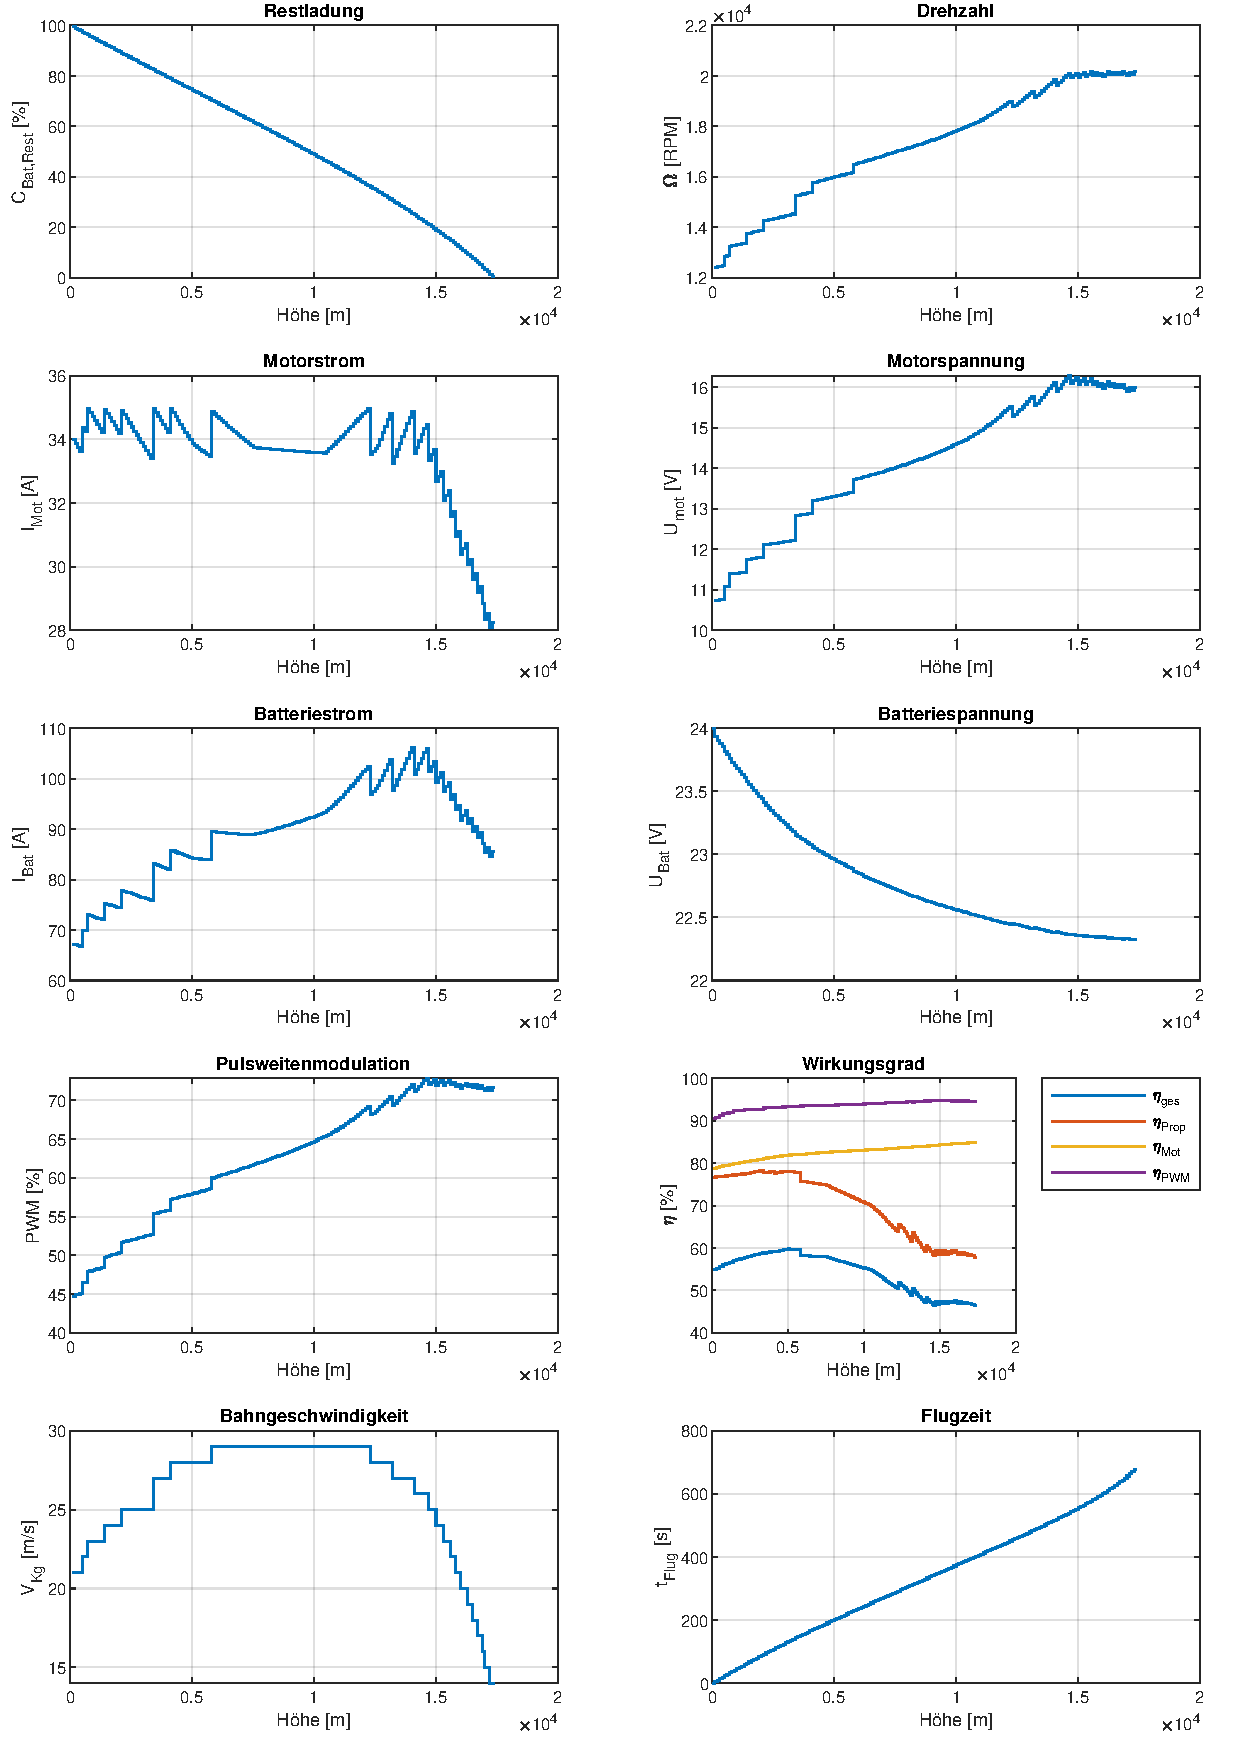
\includegraphics[scale=0.7]{Diagramme/Untersuchung_eta_pwm_halbierung_6.pdf}
	\caption{Leistungsparameter für einer Verbesserung des Motorreglerwirkungsgrades (Halbierung der Verluste) für eine Batterie mit sechs Zellen}
	\label{abb:eta_pwm_6_halb}
\end{figure}

\begin{figure}[H]
\centering
	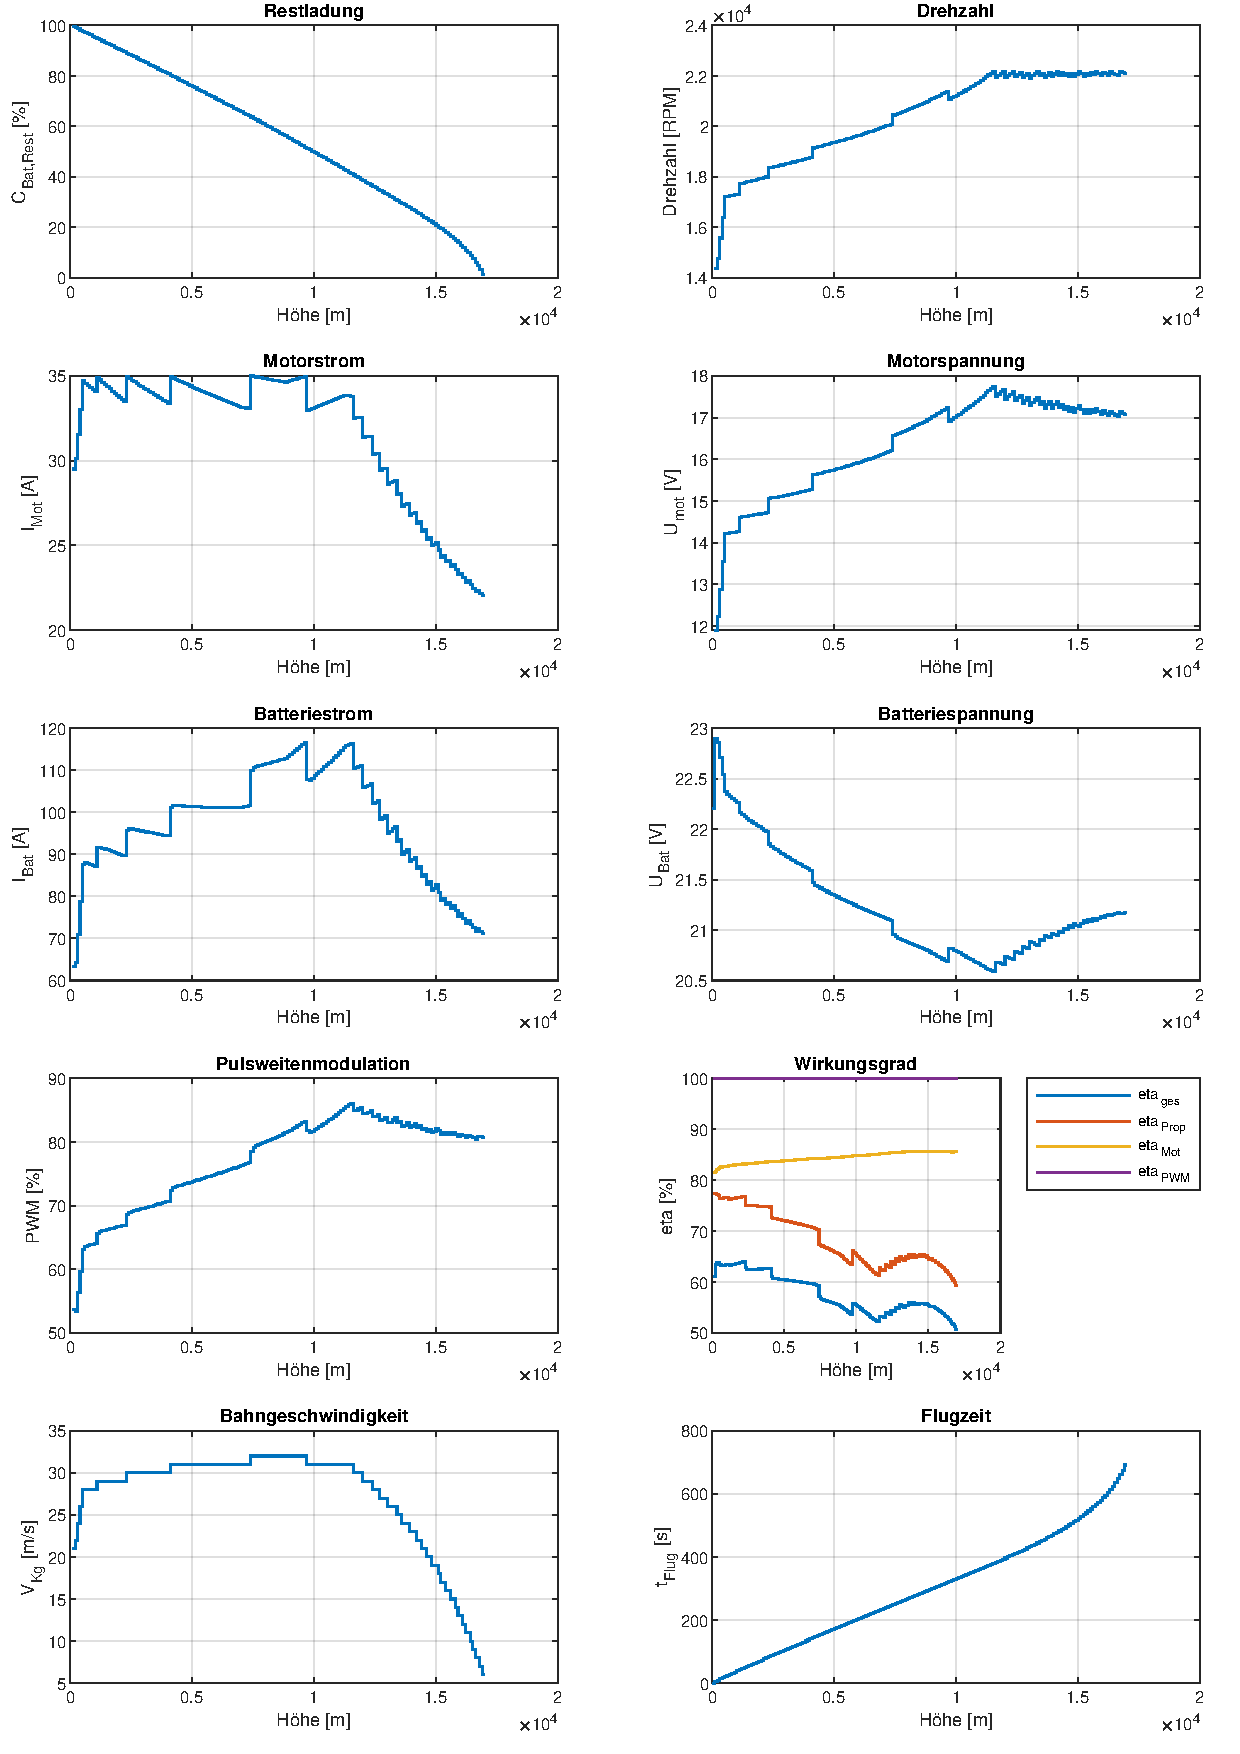
\includegraphics[scale=0.7]{Diagramme/Untersuchung_eta_pwm_1_6.pdf}
	\caption{Leistungsparameter für einer Verbesserung des Motorreglerwirkungsgrades (keine Verluste) für eine Batterie mit sechs Zellen}
	\label{abb:eta_pwm_6_1}
\end{figure}

\begin{figure}[H]
\centering
	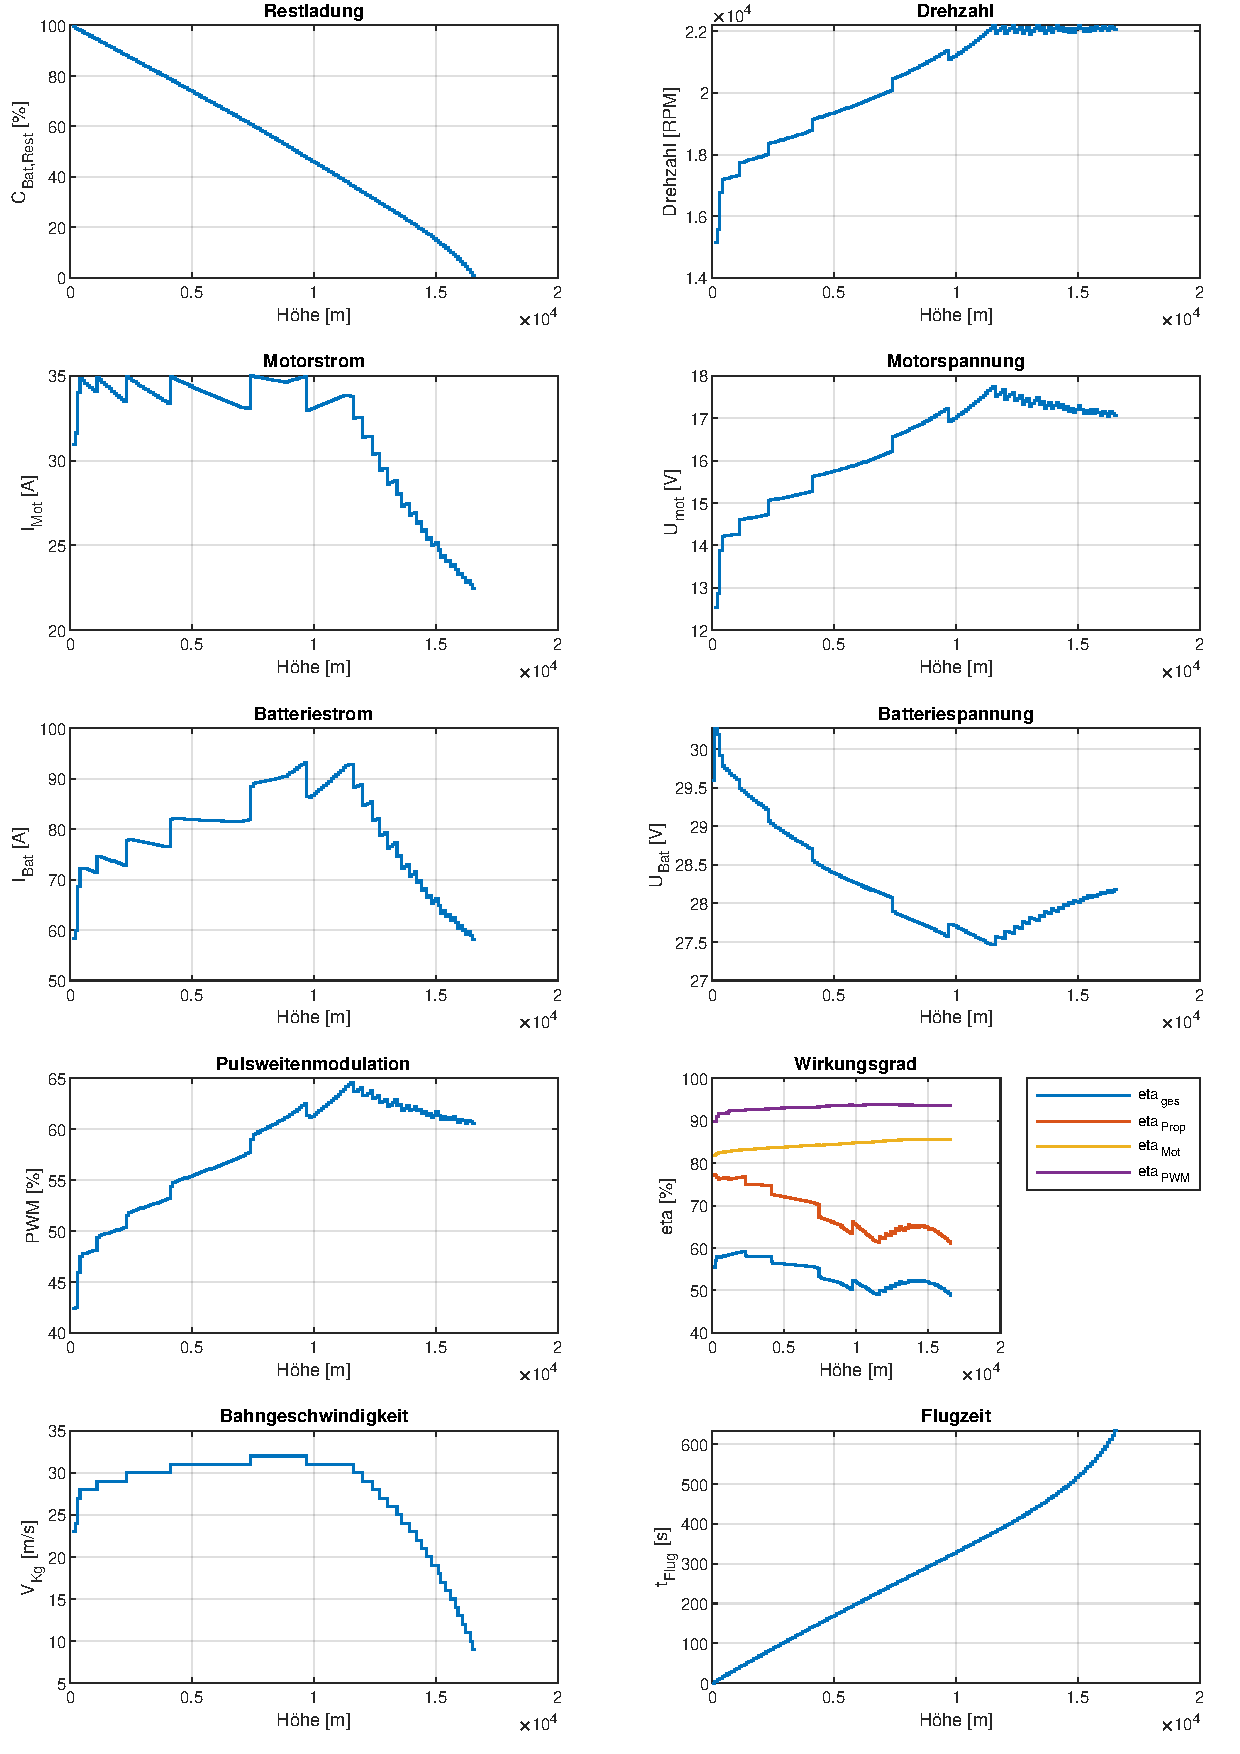
\includegraphics[scale=0.7]{Diagramme/Untersuchung_eta_pwm_halbierung_8.pdf}
	\caption{Leistungsparameter für einer Verbesserung des Motorreglerwirkungsgrades (Halbierung der Verluste) für eine Batterie mit acht Zellen}
	\label{abb:eta_pwm_8_halb}
\end{figure}

\begin{figure}[H]
\centering
	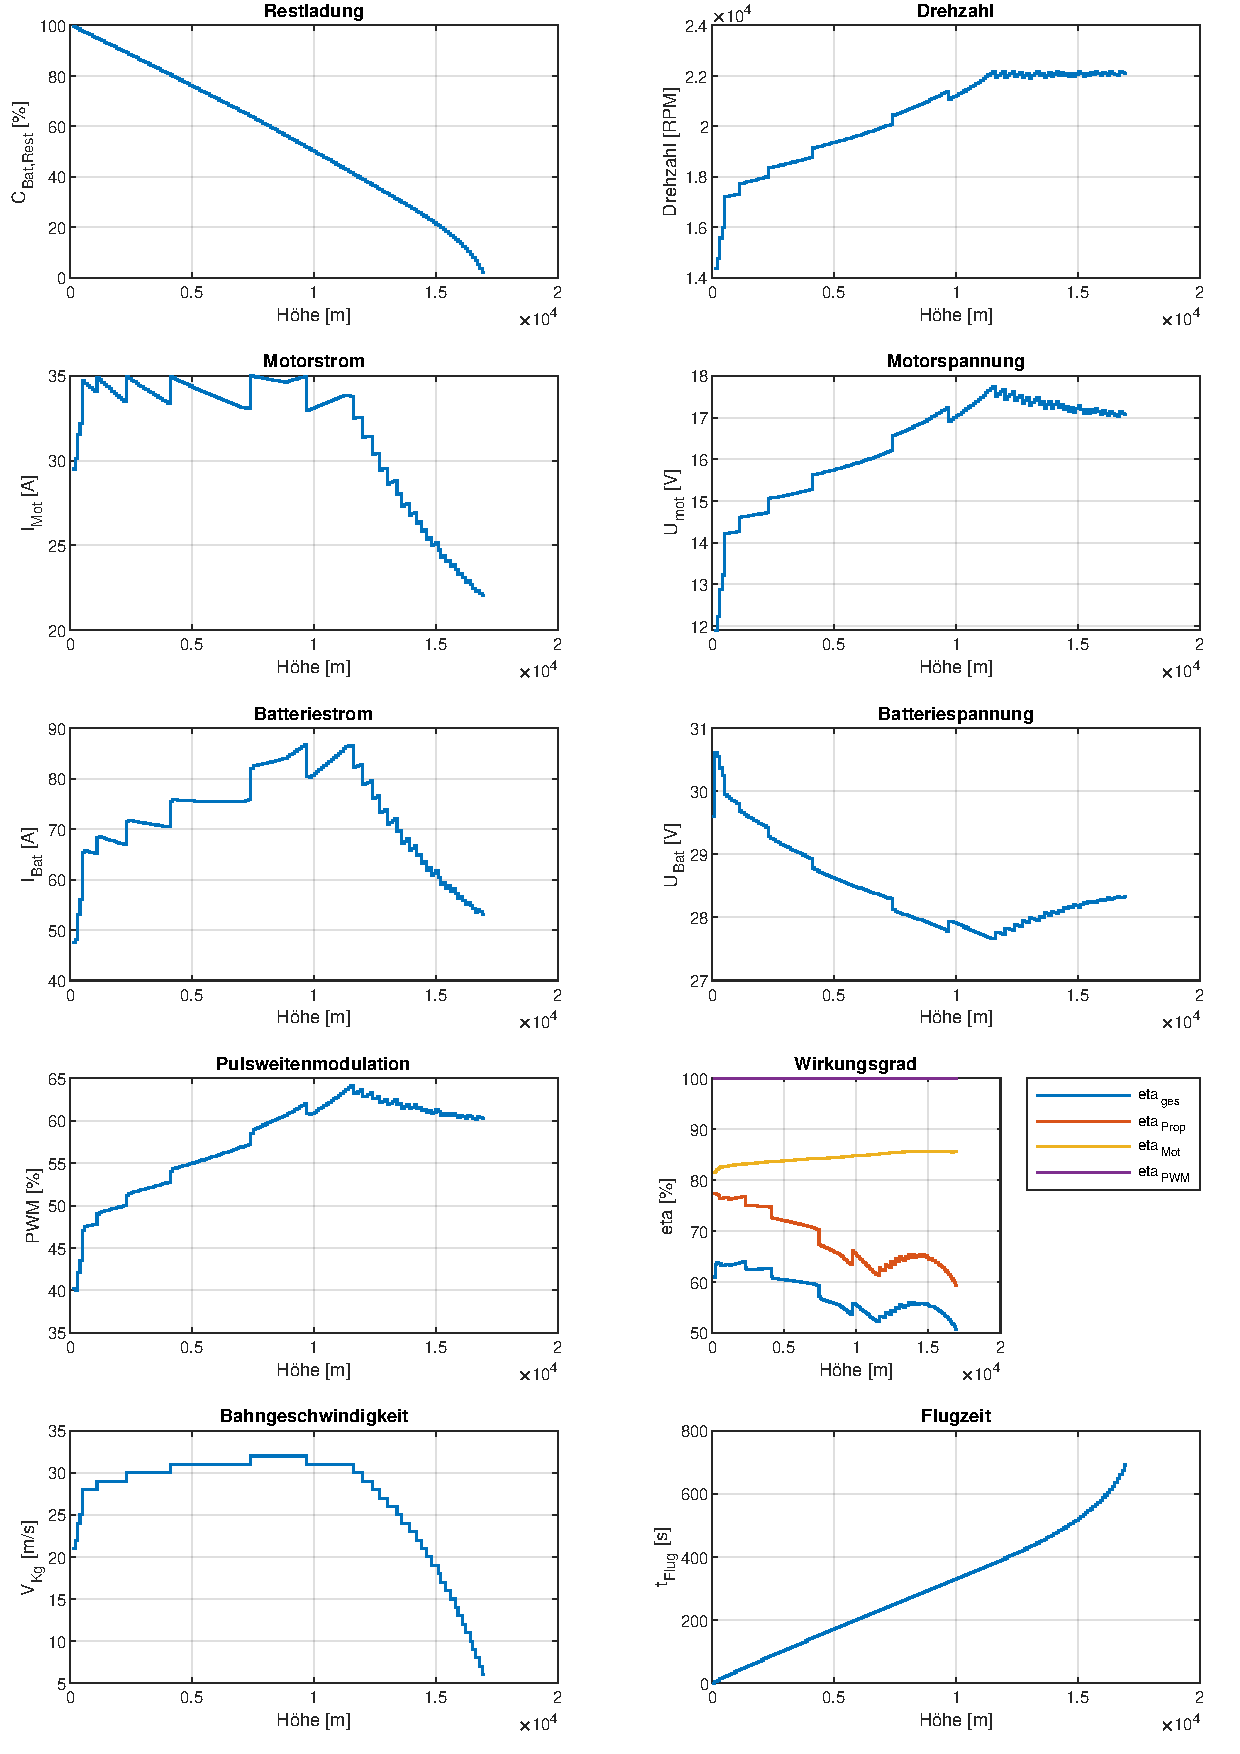
\includegraphics[scale=0.7]{Diagramme/Untersuchung_eta_pwm_1_8.pdf}
	\caption{Leistungsparameter für einer Verbesserung des Motorreglerwirkungsgrades (keine Verluste) für eine Batterie mit acht Zellen}
	\label{abb:eta_pwm_8_1}
\end{figure}



\section{Batteriemasse}
\begin{figure}[H]
\centering
	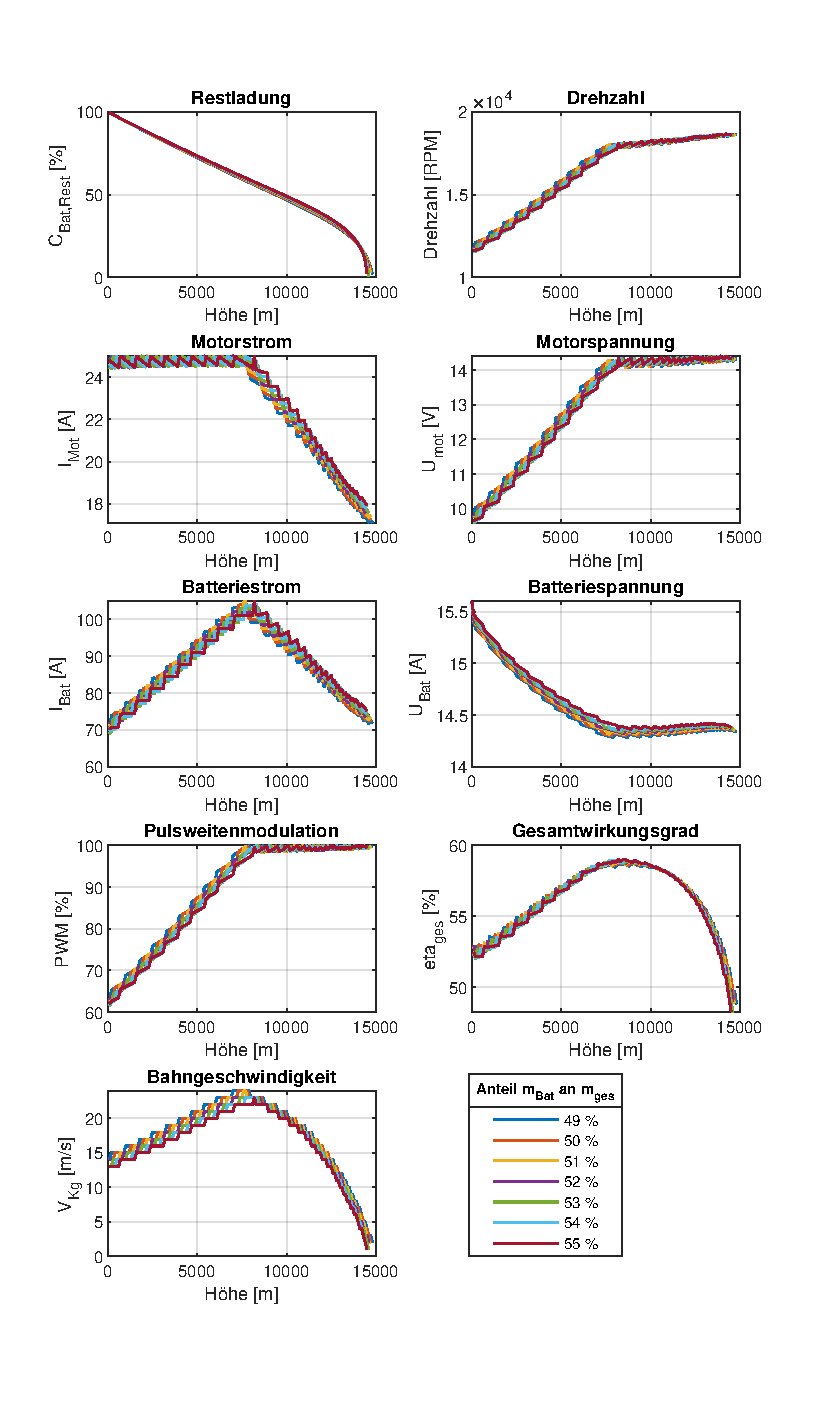
\includegraphics[scale=0.7]{Diagramme/Batteriemasse_genauer.pdf}
	\caption{genauere Untersuchung der Batteriemassenabhängigkeit (\ensuremath{m_{Mot}=\SI{106}{g}}, \ensuremath{K_V=\SI{1390}{RPM/V}}, \ensuremath{n_{Prop}=4}, \ensuremath{Propeller=\SI{10x3}{}}, \ensuremath{n_{Bat,cell}=4}, \ensuremath{u_{Wg}=\SI{10}{m/s}})}
	\label{abb:batteriemasse_genauer}
\end{figure}

\begin{figure}[H]
\centering
	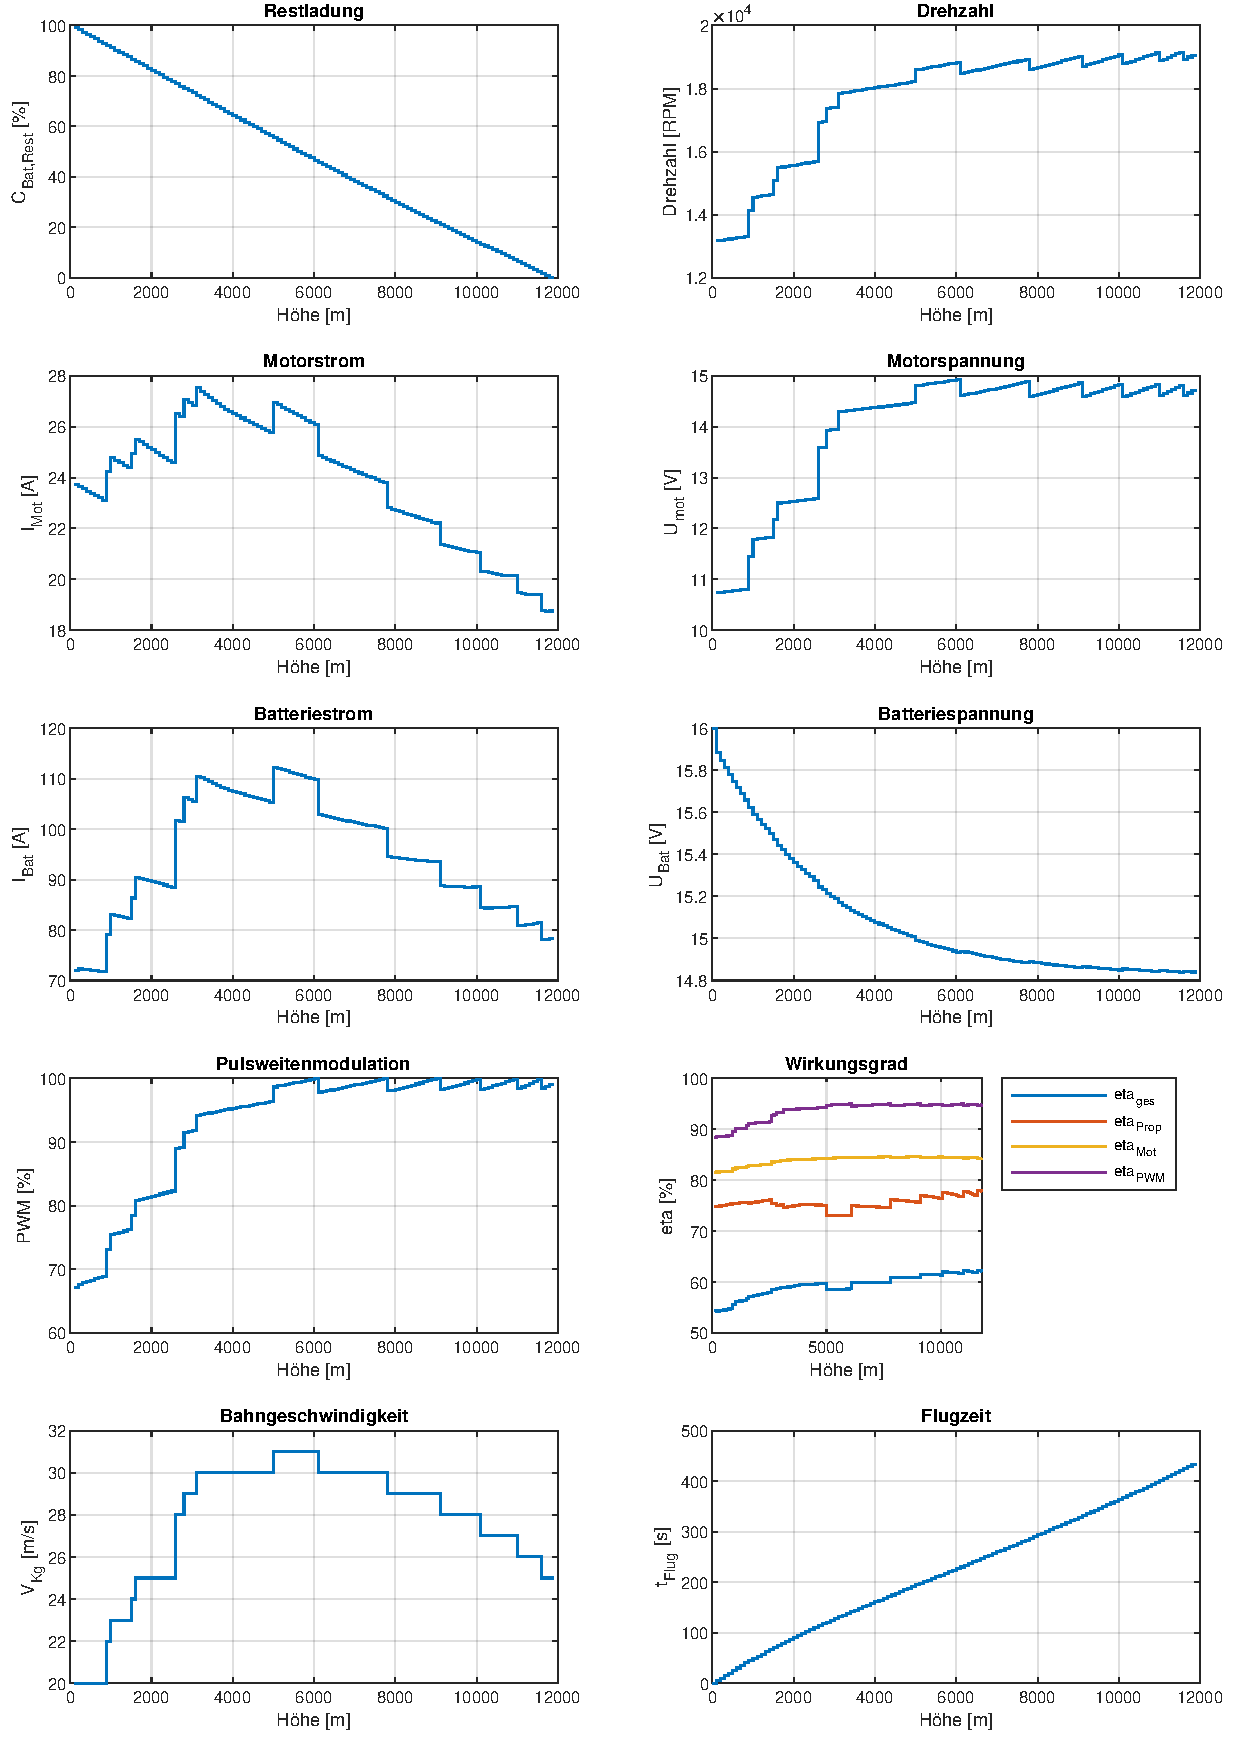
\includegraphics[scale=0.7]{Diagramme/Einfluss_eta_ges.pdf}
	\caption{Leistungsparameter für einen Batteriemassenanteil von 1/3 (\ensuremath{m_{Mot}=\SI{106}{g}}, \ensuremath{K_V=\SI{1390}{RPM/V}}, \ensuremath{n_{Prop}=4}, \ensuremath{Propeller=\SI{10x3}{}}, \ensuremath{n_{Bat,cell}=4}, \ensuremath{u_{Wg}=\SI{10}{m/s}})}
	\label{abb:m_bat_eta_ges1/3}
\end{figure}

\begin{figure}[H]
\centering
	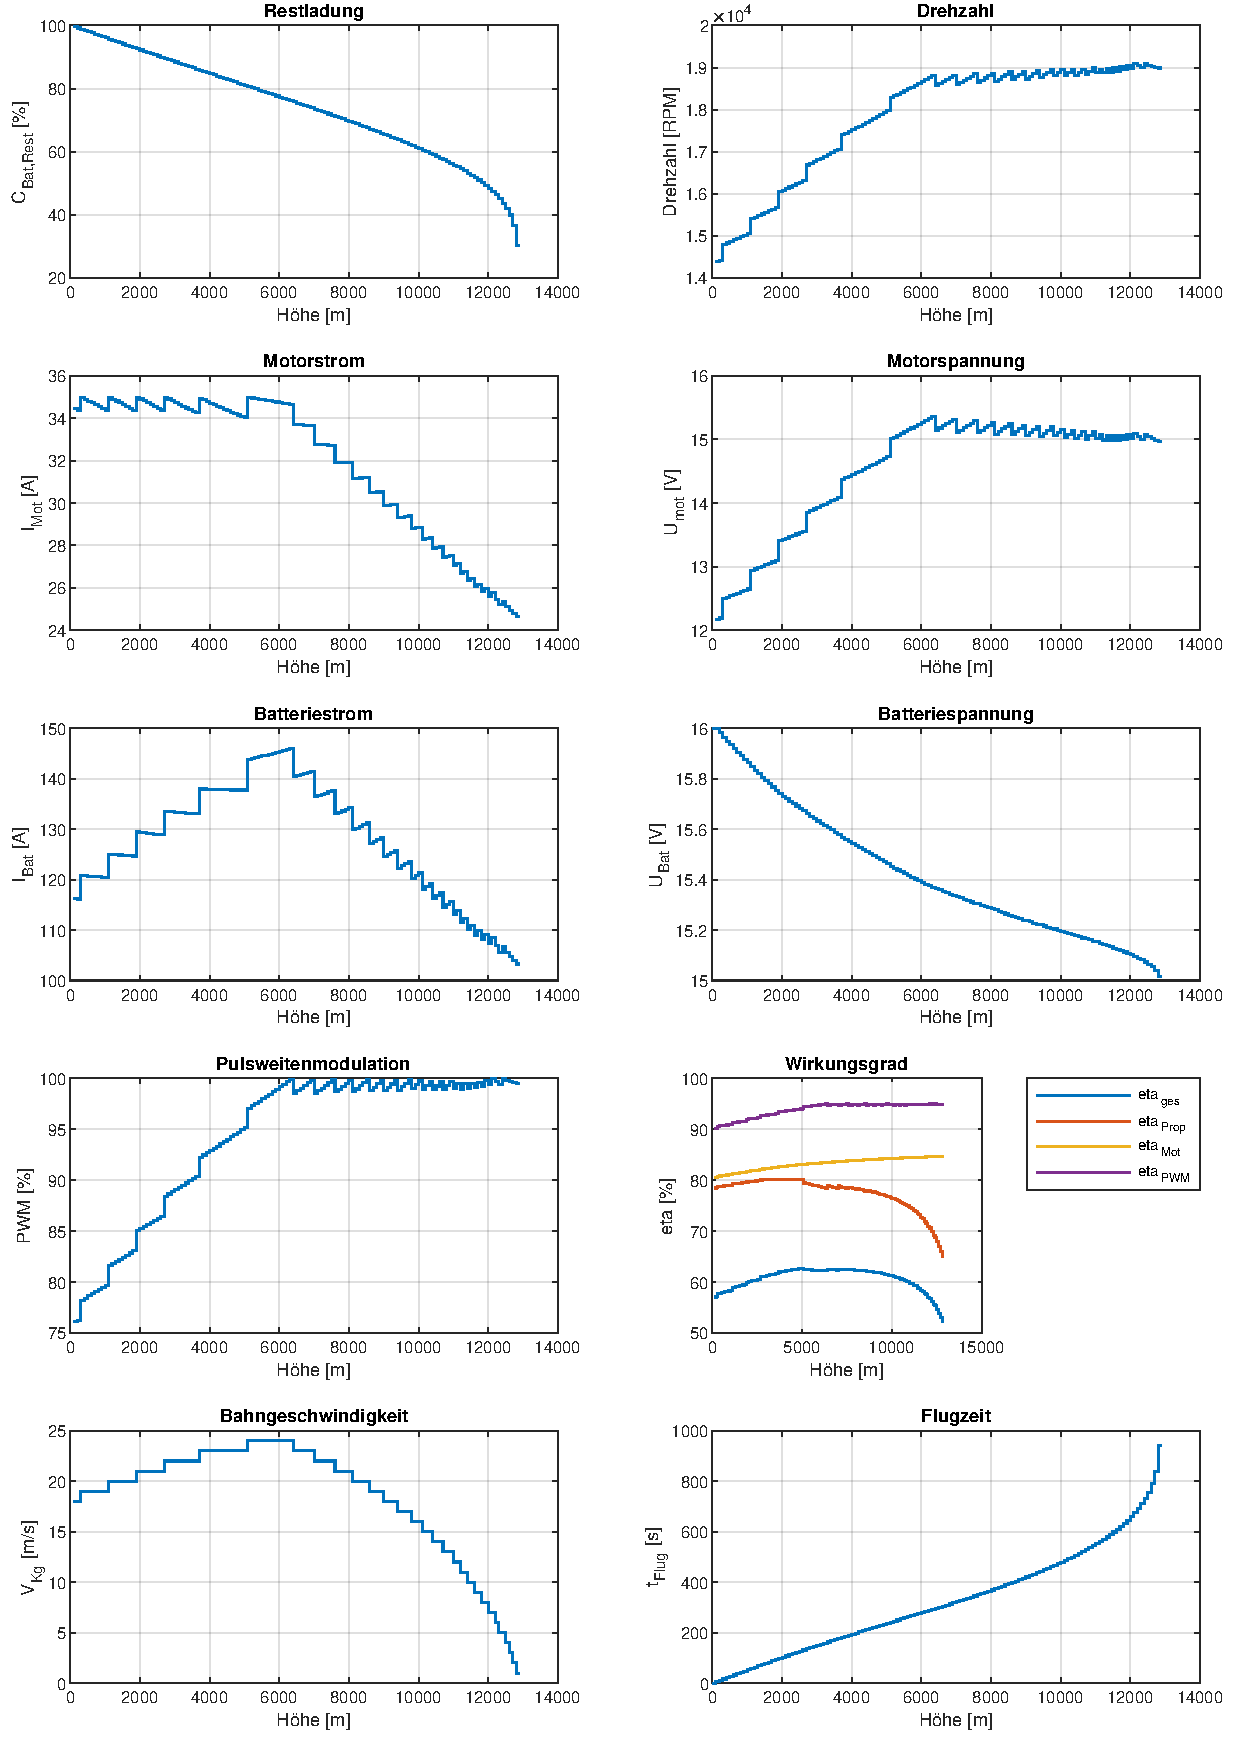
\includegraphics[scale=0.7]{Diagramme/Einfluss_eta_ges2.pdf}
	\caption{Leistungsparameter für einen Batteriemassenanteil von 2/3 (\ensuremath{m_{Mot}=\SI{106}{g}}, \ensuremath{K_V=\SI{1390}{RPM/V}}, \ensuremath{n_{Prop}=4}, \ensuremath{Propeller=\SI{10x3}{}}, \ensuremath{n_{Bat,cell}=4}, \ensuremath{u_{Wg}=\SI{10}{m/s}})}
	\label{abb:m_bat_eta_ges2/3}
\end{figure}




\section{Verstellpropeller}

\begin{center}
\begin{figure}[H]
\begin{struktogramm}(163,160)
\assign[1]{Multicopter- und Umgebungsparameter festlegen (im Startskript)}
\assign[1]{Diskretisierungen (Geschwindigkeit, Höhe) festlegen}
\assign[1]{Aufruf des Hauptskripts: Leistungsberechnung starten}
\while[5]{Für alle Zeilen der APC-Datenbank}
	\ifthenelse[10]{1}{1}{Stimmt Durchmesser mit dem gesuchten überein?}{ja}{nein}
		\assign[2]{Gehe zur nächsten Zeile}
		\change
		\assign[2]{Lösche Zeile}
	\ifend
\whileend
\while[5]{Für alle Propeller}
	\assign[2]{Extrahiere Propellerkennfeld}
	\assign[2]{Speicher das Ergebnis unter fortlaufenden Nummern}
	\assign[2]{Erhöhe Propellerzähler}
\whileend
\assign[1]{Initialisierung der Parameterberechnung}
\while[5]{F\"ur alle Höhenabschnitte}
	\assign[1]{H\"ohe, Dichte, Luftdruck Temperatur berechnen}
	\assign[1]{arithmetische Mittelwert berechnen}
	\assign[1]{Schub- und Leistungskennfeld anpassen}
	\assign[2]{Initialisierung der Leistungsberechnung}
	\while[5]{Für alle Bahngeschwindigkeiten}
		\assign[2]{Initialisierungen}
		\while[5]{Für alle Propeller}
			\assign[2]{\texttt{\textbf{Leistungsberechnung}}}
			\assign[2]{Berechnung benötigter Energiemenge bei dieser Bahngeschwindigkeit mit diesem Propeller}
		\whileend
		\ifthenelse[10]{4}{1}{Sind die Werte NaN?}{nein}{ja}
			\while[5]{Solange Abbruchkriterium nicht erreicht}		
				\assign[2]{Finde den Index mit der geringsten verbrauchten Energiemenge}
				\ifthenelse[10]{1}{1}{Werte innerhalb Leistungsgrenzen?}{ja}{nein}
				\assign[2]{Verlasse Schleife}
				\change
				\assign[2]{Suche nächst kleinere Energiemenge}
				\ifend
			\whileend
			\assign[2]{Übergabe aller Leistungsparameter mit diesem Index}
			\change
			\assign[2]{Verwerfe alle Ergebnisse}
		\ifend
		\assign[2]{Berechne benötigte Energie für Steiggeschwindigkeit}
	\whileend
	\ifthenelse[10]{4}{1}{Sind die Werte NaN?}{nein}{ja}
		\while[5]{Solange Abbruchkriterium nicht erreicht}		
			\assign[2]{Finde den Index mit der geringsten verbrauchten Energiemenge}
			\ifthenelse[10]{1}{1}{Werte innerhalb Leistungsgrenzen?}{ja}{nein}
			\assign[2]{Verlasse Schleife}
			\change
			\assign[2]{Suche nächst kleinere Energiemenge}
			\ifend
		\whileend
		\assign[2]{Übergabe aller Leistungsparameter mit diesem Index}
		\change
		\assign[2]{Verwerfe alle Ergebnisse}
	\ifend
	\assign[2]{Erhöhe Zählervariable}
\whileend
\assign[2]{Ergebnisse der Leistungsparameter in Diagrammen speichern}
\assign[2]{Speichern der Diagramme in .pdf-Datei}
\end{struktogramm}
\caption{Programmstruktur die Untersuchung des Nutzens eines Verstellpropellers}
\label{abb:vpp}
\end{figure}
\end{center}


\section{Getriebe}

\begin{center}
\begin{figure}[H]
\begin{struktogramm}(163,210)
\assign[1]{Multicopter- und Umgebungsparameter festlegen (im Startskript)}
\assign[1]{Diskretisierungen (Getriebe, Geschwindigkeit, Höhe) festlegen}
\assign[1]{Aufruf des Hauptskripts: Leistungsberechnung starten}
\assign[1]{Initialisierung der Parameterberechnung}
\while[5]{F\"ur alle Höhenabschnitte}
	\assign[1]{H\"ohe, Dichte, Luftdruck Temperatur berechnen}
	\assign[1]{arithmetische Mittelwert berechnen}
	\assign[1]{Schub- und Leistungskennfeld anpassen}
	\assign[2]{Initialisierung der Leistungsberechnung}
	\while[5]{Für alle Bahngeschwindigkeiten}
		\assign[2]{Initialisierungen}
		\while[5]{Für alle Übersetzungen}
			\assign[2]{\textbf{Leistungsberechnung}}
		\whileend
		\ifthenelse[10]{4}{1}{Sind die Werte NaN?}{nein}{ja}
			\while[5]{Solange Abbruchkriterium nicht erreicht}		
				\assign[2]{Finde den Index mit der geringsten verbrauchten Energiemenge}
				\ifthenelse[10]{1}{1}{Werte innerhalb Leistungsgrenzen?}{ja}{nein}
				\assign[2]{Verlasse Schleife}
				\change
				\assign[2]{Suche nächst kleineren Energiemenge}
				\ifend
			\whileend
			\assign[2]{Übergabe aller Leistungsparameter mit diesem Index}
			\change
			\assign[2]{Verwerfe alle Ergebnisse}
		\ifend
		\assign[2]{Berechne benötigte Energie für Steiggeschwindigkeit}
	\whileend
	\ifthenelse[10]{4}{1}{Sind die Werte NaN?}{nein}{ja}
		\while[5]{Solange Abbruchkriterium nicht erreicht}		
			\assign[2]{Finde den Index mit der geringsten verbrauchten Energiemenge}
			\ifthenelse[10]{1}{1}{Werte innerhalb Leistungsgrenzen?}{ja}{nein}
			\assign[2]{Verlasse Schleife}
			\change
			\assign[2]{Suche nächst kleinere Energiemenge}
			\ifend
		\whileend
		\assign[2]{Übergabe aller Leistungsparameter mit diesem Index}
		\change
		\assign[2]{Verwerfe alle Ergebnisse}
	\ifend
	\assign[2]{Erhöhe Zählervariable}
\whileend
\assign[2]{Ergebnisse der Leistungsparameter in Diagrammen speichern}
\assign[2]{Speichern der Diagramme in .pdf-Datei}
\end{struktogramm}
\caption{Programmstruktur die Untersuchung des Nutzens eines Getriebes}
\label{abb:getriebe}
\end{figure}
\end{center}



\end{appendix}

    \begin{appendix}
\chapter{Projektmanagement}
\label{projektmanagement}

%%%%%%%%%%%%%%%%%%%%%%%%%%%%%%%%%%%%%%%%%%%WBS%%%%%%%%%%%%%%%%%%%%%%%%%%%%%%%%%%%%%%%%%%%%

\begin{landscape}
\section{Projektstrukturplan}
% 	\captionof{Projektstrukturplan}
\label{WBS}
        \vspace{0.5cm}
        \begin{tikzpicture}[node distance=0.7cm]
            \tikzstyle{abstract}=[rectangle, draw=black, rounded corners, fill=blue!50, drop shadow,
        text centered, anchor=north, text=white, text width=3.5cm]
    \tikzstyle{topabstract}=[rectangle, draw=black, rounded corners, fill=blue!20, drop shadow,
        text centered, anchor=north, text width=0.8\linewidth]
    \tikzstyle{subabstract}=[rectangle, draw=black, rounded corners, fill=blue!20, drop shadow,
        text centered, anchor=north, text width=3.5cm]
    \tikzstyle{myarrow}=[->, >=open triangle 90, very thick]
    \tikzstyle{line}=[-, very thick]
            \node (title) [topabstract]
            {\textbf{\Large \otitle }};

            \node (AuxNode03) [text width=3.5cm, below=of title] {};
            \node (AuxNode02) [text width=3.5cm, left=of AuxNode03] {};
            \node (AuxNode01) [text width=3.5cm, left=of AuxNode02] {};
            \node (AuxNode04) [text width=3.5cm, right=of AuxNode03] {};
            \node (AuxNode05) [text width=3.5cm, right=of AuxNode04] {};
            \node (AuxNode06) [text width=3.5cm, right=of AuxNode05] {};

            \node (ap3000) [abstract, rectangle split, rectangle split parts=2, below=of AuxNode03]
                {
                    \textbf{AP 3000}
                    \nodepart{second}Überprüfung und Valdierung des Programms
                };
            \node (ap2000) [abstract, rectangle split, rectangle split parts=2, below=of AuxNode02]
                {
                    \textbf{AP 2000}
                    \nodepart{second}Programmaufbau
                };
            \node (ap1000) [abstract, rectangle split, rectangle split parts=2, below=of AuxNode01]
                {
                    \textbf{AP 1000}
                    \nodepart{second}Literaturrecherche
                };
            \node (ap4000) [abstract, rectangle split, rectangle split parts=2, below=of AuxNode04]
                {
                    \textbf{AP 4000}
                    \nodepart{second}Parameteruntersuchung
                };
            \node (ap5000) [abstract, rectangle split, rectangle split parts=2, below=of AuxNode05]
                {
                    \textbf{AP 5000}
                    \nodepart{second}Auswertung
                };
            \node (ap1100) [subabstract, rectangle split, rectangle split parts=2, below=of ap1000]
                {
                    \textbf{AP 1100}
                    \nodepart{second}Flugmechanik und Aerodynamik von Multicoptern und Flächenflugzeugen
                };
            \node (ap1200) [subabstract, rectangle split, rectangle split parts=2, below=of ap1100]
                {
                    \textbf{AP 1200}
                    \nodepart{second}Zusammenhang einer elektromechanischen Antriebseinheit
                };
            \node (ap2100) [subabstract, rectangle split, rectangle split parts=2, below=of ap2000]
                {
                    \textbf{AP 2100}
                    \nodepart{second}Erstellung eines Modells in Matlab
                };
            \node (ap2200) [subabstract, rectangle split, rectangle split parts=2, below=of ap2100]
                {
                    \textbf{AP 2200}
                    \nodepart{second}Programmablauf
                };
            \node (ap3100) [subabstract, rectangle split, rectangle split parts=2, below=of ap3000]
               {
                   \textbf{AP 3100}
                   \nodepart{second}Nachbildung eines Quadrocopterfluges im Programm
               };
               \node (ap3200) [subabstract, rectangle split, rectangle split parts=2, below=of ap3100]
               {
                   \textbf{AP 3200}
                   \nodepart{second}Diskussion der Flugleistungen
               };
            \node (ap4100) [subabstract, rectangle split, rectangle split parts=2, below=of ap4000]
               {
                   \textbf{AP 4100}
                   \nodepart{second}Festlegung der zu untersuchenden Parameter und wie diese zu variieren sind
               };
            \node (ap4200) [subabstract, rectangle split, rectangle split parts=2, below=of ap4100]
               {
                   \textbf{AP 4200}
                   \nodepart{second}Programmerweiterung
                   };
            \node (ap4300) [subabstract, rectangle split, rectangle split parts=2, below=of ap4200]
                {
                    \textbf{AP 4300}
                    \nodepart{second}Einflussuntersuchung der Parameter
                };
            \node (ap5100) [subabstract, rectangle split, rectangle split parts=2, below=of ap5000]
                {
                    \textbf{AP 5100}
                    \nodepart{second}Diskussion der Ergebnisse
                };
%			 \node (ap5200) [subabstract, rectangle split, rectangle split parts=2, below=of ap5100]
%                {
%                    \textbf{AP 5200}
%                    \nodepart{second}Ausblick
%                };
            \node (AuxNode06) [text width=3.5cm, below=of ap5100] {};
            \node (ap6000) [abstract, rectangle split, rectangle split parts=2, below=of AuxNode06]
                {
                    \textbf{AP 6000}
                    \nodepart{second}Dokumentation
                };

            \draw[myarrow]  (ap5000.north) -- ++(0,0.8) -| (title.south);
            \draw[line] (ap5000.north) -- ++(0,0.8) -| (ap4000.north);
            \draw[line] (ap5000.north) -- ++(0,0.8) -| (ap3000.north);
            \draw[line] (ap5000.north) -- ++(0,0.8) -| (ap2000.north);
            \draw[line] (ap5000.north) -- ++(0,0.8) -| (ap1000.north);
            \draw[line] (ap5000.north) -- ++(0,0.8) -| (ap1000.north);
            \draw[line] (ap1000.west)  -- ++(-0.19,0);
            \draw[line] (ap1100.west)  -- ++(-0.2,0);
            \draw[line] (ap1200.west)  -- ++(-0.2,0) -- ([yshift=0.0cm, xshift=-0.19cm] ap1000.west);
            \draw[line] (ap2000.west)  -- ++(-0.19,0);
            \draw[line] (ap2100.west)  -- ++(-0.2,0);
            \draw[line] (ap2200.west)  -- ++(-0.2,0) -- ([yshift=0.0cm, xshift=-0.19cm]ap2000.west);
			\draw[line] (ap3000.west) -- ++(-0.19,0);
            \draw[line] (ap3100.west) -- ++(-0.2,0);
            \draw[line] (ap3200.west) -- ++(-0.2,0) -- ([yshift=0.0cm, xshift=-0.19cm]ap3000.west);
            \draw[line] (ap4000.west) -- ++(-0.19,0);
            \draw[line] (ap4100.west) -- ++(-0.2,0);
            \draw[line] (ap4200.west) -- ++(-0.2,0);
            \draw[line] (ap4300.west) -- ++(-0.2,0) -- ([yshift=0.0cm, xshift=-0.19cm] ap4000.west);
            \draw[line] (ap5000.west) -- ++(-0.19,0);
            \draw[line] (ap5100.west) -- ++(-0.2,0) -- ([yshift=0.0cm, xshift=-0.19cm] ap5000.west);
            \draw[line] (ap6000.east) -- ++(+0.2,0) |- ([yshift=0.8cm, xshift=0.00cm] ap5000.north);
        \end{tikzpicture}
%    \end{center}
%\end{sidewaystable}
\end{landscape}

%%%%%%%%%%%%%%%%%%%%%%%%%%%%%%%%%%%% Zeitplan %%%%%%%%%%%%%%%%%%%%%%%%%%%%%%%%%%%%%%%%%%%%%%

\begin{landscape}
\section{Zeitplan}
\label{sec:zeitplan}
\noindent\resizebox{\linewidth}{!}{	% Einfügen, falls zu groß
\begin{ganttchart}[hgrid,
                   time slot format = isodate,
                   x unit=0.2cm,	% Zum komprimieren des Charts in x-Richtung
                   y unit chart=1.05cm,
                   %compress calendar,	% Komprimiert den Chart in der Breite
                   calendar week text = {\currentweek},
                   chart element start border = right,
                   bar/.append style={fill=blue!40, rounded corners=2pt},
                   bar incomplete/.append style={fill=blue!10},
                   bar label node/.append style={align=left, text width=7cm},
                   group label node/.append style={align=left, text width=8cm},
                   milestone label node/.append style={align=left, text width=8cm},
                   bar progress label node/.style={right=2mm},
                   progress label text = {\pgfmathprintnumber[precision=0, verbatim]{#1}\%},
                  ]{2018-11-15}{2019-03-01}
  \gantttitlecalendar{year, month=shortname, week}\\
  %\gantttitle{2013}{59}\\
  \ganttgroup{AP 1000: Literaturrecherche}{2018-11-27}{2018-12-04}\\
  \ganttbar  {AP 1100: Flugmechanik und Aerodynamik von Multicoptern und Flächenflugzeugen}{2018-11-27}{2018-11-30}\\
  \ganttlinkedbar [link type=rdldr, link mid = 0.6, link bulge = 3]{AP 1200: Zusammenhang einer elektromechanischen Antriebseinheit}{2018-12-01}{2018-12-04}\\
  %\ganttbar[progress=100]{AP 1300: TEXT}{2013-01-01}{2013-01-30}\\	% Beispiel für Fortschrittsbalken!

  \ganttgroup{AP 2000: Programmaufbau}{2018-12-05}{2018-12-20}\\
  \ganttbar  {AP 2100: Erstellung eines Modells in Matlab}{2018-12-05}{2018-12-17}\\
  \ganttlinkedbar [link type=rdldr, link mid = 0.6, link bulge = 3] {AP 2200: Struktogramm}{2018-12-14}{2018-12-20}\\

  \ganttgroup{AP 3000: Überprüfung und Valdierung des Programms}{2018-12-21}{2018-12-28}\\
  \ganttbar  {AP 3100: Modellierung eines Quadrocopterfluges im Programm}{2018-12-21}{2018-12-22}\\
  \ganttlinkedbar [link type=rdldr, link mid = 0.6, link bulge = 3] {AP 3200: Diskussion der Flugleistungen}{2018-12-23}{2018-12-28}\\

  \ganttgroup{AP 4000: Parameteruntersuchung}{2019-01-02}{2019-02-07}\\
  \ganttbar{AP 4100: Festlegung der zu untersuchenden Parameter und wie diese zu variieren sind}{2019-01-02}{2019-01-09}\\
  \ganttlinkedbar [link type=rdldr, link mid = 0.6, link bulge = 3] {AP 4200: Programmerweiterung}{2019-01-10}{2019-02-07}\\
  \ganttlinkedbar [link type=rdldr, link mid = 0.6, link bulge = 3] {AP 4300: Einflussuntersuchung der Parameter}{2019-01-10}{2019-02-07}\\

  \ganttgroup{AP 5000: Auswertung}{2019-02-08}{2019-02-22}\\
  \ganttbar  {AP 5100: Diskussion der Ergebnisse}{2019-02-08}{2019-02-22}\\

  \ganttgroup{AP 6000: Dokumentation}{2018-12-04}{2019-02-22}\\
  %\ganttmilestone{Meilenstein}{2013-02-20}\\

 \end{ganttchart}
}
\end{landscape}


%%%%%%%%%%%%%%%%%%%%%%%%%%%%%%%%%%% WPD %%%%%%%%%%%%%%%%%%%%%%%%%%%%%%%%%%%%%%%%%%%%%%%%%%

% WPD 1100

\clearpage
\begin{wpd}{AP 1100}{Flugmechanik und Aerodynamik von Multicoptern und Flächenflugzeugen}{1.0}{Lucas Schreer}{26.11.2018}{27.11.2018}{31.11.2018}{5 Tage}{Lucas Schreer}
    {
    \textbf{Ziele:}
    \begin{itemize}
        \item grundlegende Berechnung der Flugleistungen eines Multicopters
        \item vereinfachte Berechnung der Flugleistungen eines Flächenflugzeugs
        \item Kenntnis über flugmechanische Zusammenhänge
    \end{itemize}
    \textbf{Input:}
    \begin{itemize}
        \item Literaturrecherche bezüglich der Flugmechanik und Aerodynamik von Hubschraubern und Flächenflugzeugen
    \end{itemize}
    \textbf{Schnittstellen zu anderen APs:}
    \begin{itemize}
        \item AP 2100
        \item AP 5200
    \end{itemize}
    \textbf{Aufgaben:}
    \begin{itemize}
        \item Literaturrecherche
        \item Einlesen in die Thematik der Aerodynamik von Hubschraubern sowie Flächenflugzeugen
    \end{itemize}
    \textbf{Ergebnisse:}
    \begin{itemize}
        \item Kenntnis über grundsätzliche flugmechanische und aerodynamische Zusammenhänge von Multicoptern bzw. Flächenflugzeugen
        \item Wissen über die Genauigkeit der getroffenen Annahmen sowie die Grenzen der Genauigkeit
    \end{itemize}
    }
\end{wpd}

% WPD 1200

\clearpage
\begin{wpd}{AP 1200}{Zusammenhang einer elektromechanischen Antriebseinheit}{1.0}{Lucas Schreer}{26.11.2018}{01.12.2018}{04.12.2018}{4 Tage}{Lucas Schreer}
    {
    \textbf{Ziele:}
    \begin{itemize}
        \item Kenntnis über elektromechanische Antriebseinheiten
        \item Wissen über die gegenseitige Beeinflussung der Antriebseinheiten
    \end{itemize}
    \textbf{Input:}
    \begin{itemize}
        \item Literaturrecherche bezüglich Brushlessmotoren, Reglern, Batterien , etc.
    \end{itemize}
    \textbf{Schnittstellen zu anderen APs:}
    \begin{itemize}
        \item AP 2100, AP 4000
    \end{itemize}
    \textbf{Aufgaben:}
    \begin{itemize}
        \item Auseinandersetzung mit der Thematik 
        \item Kenntnis über die Grundlagen eines elektromechanischen Antriebs        
    \end{itemize}
    \textbf{Ergebnisse:}
    \begin{itemize}
        \item Kenntnis über den Zusammenhang und die Berechnung einzelner Komponenten der elektrischen Antriebseinheit
        \item Wissen über die Grenzen der elektromechanischen Einheiten
    \end{itemize}
    }
\end{wpd}

%WPD 2100

\clearpage
\begin{wpd}{AP 2100}{Erstellung eines Modells in Matlab}{1.0}{Lucas Schreer}{27.11.2018}{05.12.2018}{17.12.2018}{2 Wochen}{Lucas Schreer}
    {
    \textbf{Ziele:}
    \begin{itemize}
        \item Implementierung der Flugmechanik und Aerodynamik von Multicoptern und Flächenflugzeugen in Matlab
        \item Implementierung des elektromechanischen Antriebsstrangs
    \end{itemize}
    \textbf{Input:}
    \begin{itemize}
        \item Ergebnisse aus AP 1100 und AP 1200
    \end{itemize}
    \textbf{Schnittstellen zu anderen APs:}
    \begin{itemize}
        \item AP 4300
    \end{itemize}
    \textbf{Aufgaben:}
    \begin{itemize}
    	\item Implementierung der Zusammenhänge zwischen Aerodynamik, Flugmechanik und der elektrischen Antriebseinheit
    	\item Anfertigen eines organisierten Programmablaufs von der Aerodynamik zur Batterieentladung
    	\item Darstellung der Ergebnisse in geeigneten Diagrammen
    \end{itemize}
    \textbf{Ergebnisse:}
    \begin{itemize}
        \item Ein geeignetes Programm für fortlaufende Untersuchungen und anschließende Programmerweiterung
        \item Fertiges Matlab Programm zur Durchführung einer ersten Simulationen von elektrisch angetriebenen Flugsystemen mit einer Bandbreite von Parametern sowie deren Auswertung
    \end{itemize}
    }
\end{wpd}

% WPD 2200

\clearpage
\begin{wpd}{AP 2200}{Struktogramm}{1.0}{Lucas Schreer}{26.11.2018}{14.12.2018}{20.12.2018}{7 Tage}{Lucas Schreer}
    {
    \textbf{Ziele:}
    \begin{itemize}
        \item Erstellen eines Struktogramms für das Programm zur Leistungsberechnung
    \end{itemize}
    \textbf{Input:}
    \begin{itemize}
        \item Ergebnisse aus AP 2100
    \end{itemize}
    \textbf{Schnittstellen zu anderen APs:}
    \begin{itemize}
        \item AP 6000
    \end{itemize}
    \textbf{Aufgaben:}
    \begin{itemize}
        \item Erstellen eines Struktogramms für die einzelnen Programmabläufe
        \item Überprüfung des Programmablaufs auf Optimierungspotenzial
    \end{itemize}
    \textbf{Ergebnisse:}
    \begin{itemize}
        \item Strukturiertes Ablaufdiagramm, welches die entsprechenden Abläufe ohne Quelltext darstellt
        \item Optimierung der Programmablaufstruktur
    \end{itemize}
    }
\end{wpd}

% WPD 3100

\clearpage
\begin{wpd}{AP 3100}{Nachbildung eines Quadrocopterfluges im Programm}{1.0}{Lucas Schreer}{26.11.2018}{21.12.2018}{22.12.2018}{2 Tage}{Lucas Schreer}
    {
    \textbf{Ziele:}
    \begin{itemize}
        \item Überprüfung der Validität des Quadrocopterfluges in Russland
        \item Validierung des aufgestellten Modells
    \end{itemize}
    \textbf{Input:}
    \begin{itemize}
        \item Ergebnisse aus AP 2100
    \end{itemize}
%    \textbf{Schnittstellen zu anderen APs:}
%    \begin{itemize}
%        \item AP 3200
%    \end{itemize}
    \textbf{Aufgaben:}
    \begin{itemize}
        \item Internetrecherche aller benötigten Parameter zur Nachbildung des Fluges im Programm
        \item Darstellung der nachgebildeten Flugleistungen in Diagrammen
    \end{itemize}
    \textbf{Ergebnisse:}
    \begin{itemize}
        \item Nachgebildeter Flug im Programm
    \end{itemize}
    }
\end{wpd}

% WPD 3200

\clearpage
\begin{wpd}{AP 3200}{Diskussion der Flugleistungen}{1.0}{Lucas Schreer}{26.11.2018}{23.12.2018}{28.12.2018}{3 Tage}{Lucas Schreer}
    {
    \textbf{Ziele:}
    \begin{itemize}
        \item Überprüfung der angegebenen Flugleistungen mit dem Programm
        \item Validierung des aufgestellten Modells
    \end{itemize}
    \textbf{Input:}
    \begin{itemize}
        \item Ergebnisse aus AP 3100
    \end{itemize}
    \textbf{Schnittstellen zu anderen APs:}
    \begin{itemize}
        \item AP 3100
    \end{itemize}
    \textbf{Aufgaben:}
    \begin{itemize}
        \item Abgleichen der Flugleistungen des Programms mit den im Video gezeigten
        \item Logische Prüfung der Ergebnisse in Bezug auf die Umsetzung
        \item Nachvollziehen und Klären der Plausibilität der im Video gezeigten Flugleistungen
    \end{itemize}
    \textbf{Ergebnisse:}
    \begin{itemize}
        \item Aussagen zur Validität des aufgestellten Modells
    \end{itemize}
    }
\end{wpd}

% WPD 4100

\clearpage
\begin{wpd}{AP 4100}{Festlegung der zu untersuchenden Parameter und wie diese zu variieren sind}{1.0}{Lucas Schreer}{26.11.2018}{02.01.2019}{09.01.2019}{1 Woche}{Lucas Schreer}
    {
    \textbf{Ziele:}
    \begin{itemize}
        \item Liste mit allen zu untersuchenden und variierenden Parametern
        \item Wissen um die Implementierung im Modell
    \end{itemize}
    \textbf{Input:}
    \begin{itemize}
        \item Ergebnisse aus AP100, AP 2000 und AP 3000
    \end{itemize}
    \textbf{Schnittstellen zu anderen APs:}
    \begin{itemize}
        \item AP 4200 und AP 4300
    \end{itemize}
    \textbf{Aufgaben:}
    \begin{itemize}
        \item Herausfiltern relevanter Parameter
        \item Suchen nach Möglichkeiten zur Variation der Parameter
        \item Vorabeinschätzung der Relevanz für die Flugleistungen
        \item Klärung eventueller Interferenzen
    \end{itemize}
    \textbf{Ergebnisse:}
    \begin{itemize}
        \item Anzahl an zu untersuchenden Parameter und sinnvolle Variation dieser
        \item mögliche Zusammenhänge einzelner Parameter
        \item grobe Programmablaufsequenzen zur Untersuchung der Parameter 
    \end{itemize}
    }
\end{wpd}

% WPD 4200

\clearpage
\begin{wpd}{AP 4200}{Programmerweiterung}{1.0}{Lucas Schreer}{26.11.2018}{10.01.2019}{07.02.2019}{4 Wochen}{Lucas Schreer}
    {
    \textbf{Ziele:}
    \begin{itemize}
        \item Erweiterung und Anpassung des Programms um neue Aspekte der Parameteruntersuchung
    \end{itemize}
    \textbf{Input:}
    \begin{itemize}
        \item Ergebnisse aus AP 2000 und AP 4100
    \end{itemize}
    \textbf{Schnittstellen zu anderen APs:}
    \begin{itemize}
        \item AP 2100
    \end{itemize}
    \textbf{Aufgaben:}
    \begin{itemize}
        \item Einbau weiterer Programmstrukturen, die die Untersuchung der in AP 4100 aufgestellten Parameter ermöglichen
        \item Erweiterung des Programms um Strukturen zur Visualisierung der Ergebnisse
    \end{itemize}
    \textbf{Ergebnisse:}
    \begin{itemize}
        \item Erweitertes und an die Untersuchung angepasstes Programm 
        \item Funktionen und Iterationen, die eine Parameteruntersuchung ermöglichen  
    \end{itemize}
    }
\end{wpd}

% WPD 4300 

\clearpage
\begin{wpd}{AP 4300}{Einflussuntersuchung der Parameter}{1.0}{Lucas Schreer}{26.11.2018}{10.01.2019}{07.02.2019}{4 Wochen}{Lucas Schreer}
    {
    \textbf{Ziele:}
    \begin{itemize}
        \item Untersuchung des Einflusses der in AP 4100 festgelegten Parameter
    \end{itemize}
    \textbf{Input:}
    \begin{itemize}
        \item Ergebnisse aus AP 4100 und AP 4200
    \end{itemize}
    \textbf{Schnittstellen zu anderen APs:}
    \begin{itemize}
        \item AP 2000
    \end{itemize}
    \textbf{Aufgaben:}
    \begin{itemize}
        \item Untersuchung des Parametereinflusses auf die Flugleistungen des Flugsystems
        \item Darstellung dieses Einflusses in dafür geeigneten Diagrammen, Graphen, Bildern, etc.
    \end{itemize}
    \textbf{Ergebnisse:}
    \begin{itemize}
        \item Aufzeigen des Einflusses auf die Flugleistungen
        \item Ermittlung des Optimums für die Flugleistung
    \end{itemize}
    }
\end{wpd}

% WPD 5100 

\clearpage
\begin{wpd}{AP 5100}{Diskussion der Ergebnisse}{1.0}{Lucas Schreer}{26.11.2018}{08.02.2019}{22.02.2019}{2 Woche}{Lucas Schreer}
    {
    \textbf{Ziele:}
    \begin{itemize}
        \item Festhalten der optimalen Parameter zur Erfüllung der Mission
        \item Bewertung der Ergebnisse im Hinblick auf Korrektheit und technischer Realisierbarkeit
        \item Empfehlungen für die optimale Auslegung eines Flugsystems für einen Steiglug auf \SI{10}{km} Höhe
    \end{itemize}
    \textbf{Input:}
    \begin{itemize}
        \item Ergebnisse aus AP 4200 und AP 4300
    \end{itemize}
    \textbf{Schnittstellen zu anderen APs:}
    \begin{itemize}
        \item AP 4000
    \end{itemize}
    \textbf{Aufgaben:}
    \begin{itemize}        
        \item Kritische Betrachtung der Ergebnisse und der gemachten Angaben 
        \item Auswertung der Ergebnisse im Hinblick auf die bestmöglichen Flugeigenschaften
    \end{itemize}
    \textbf{Ergebnisse:}
    \begin{itemize}
        \item Aussagen über eine bestmögliche Konstellation der Flugsystemparameter zum Erreichen einer Höhe von \SI{10}{km} oder sogar \SI{15}{km}
        \item Aussagen über die Realisierbarkeit 
        \item Wissen um die Abweichungen von der Realität und deren Einfluss 
        \item Ausblick auf zukünftige Entwicklungen
    \end{itemize}
    }
\end{wpd}

% WPD 5200

%\clearpage
%\begin{wpd}{AP 5200}{Ausblick}{1.0}{Lucas Schreer}{26.11.2019}{15.02.2019}{20.02.2019}{5 Tage}{Lucas Schreer}
%    {
%    \textbf{Ziele:}
%    \begin{itemize}
%        \item 
%    \end{itemize}
%    \textbf{Input:}
%    \begin{itemize}
%        \item Ergebnisse aus AP 5100 und AP 5300
%    \end{itemize}
%   	\textbf{Schnittstellen zu anderen APs:}
%  	\begin{itemize}
%        \item AP 5000
%	\end{itemize}
%    \textbf{Aufgaben:}
%    \begin{itemize}
%    	\item
%    \end{itemize}
%    \textbf{Ergebnisse:}
%    \begin{itemize}
%        \item Ausblick auf zukünftige Entwicklungen
%    \end{itemize}
%    }
%\end{wpd}

% WPD 6000

\clearpage
\begin{wpd}{AP 6000}{Dokumentation}{1.0}{Lucas Schreer}{26.11.2018}{04.12.2018}{22.02.2019}{11 Wochen}{Lucas Schreer}
    {
    \textbf{Ziele:}
    \begin{itemize}
        \item Schriftliche Dokumentation der Arbeit
    \end{itemize}
    \textbf{Input:}
    \begin{itemize}
        \item AP 1000
        \item AP 2000
        \item AP 3000
        \item AP 4000
        \item AP 5000
    \end{itemize}
    \textbf{Aufgaben:}
    \begin{itemize}
        \item Einarbeitung in Zeichensatzprogramme, wie \LaTeX, {\fontfamily{cmr}Ti{\em k}Z}, \emph{PGF} und \emph{Gnuplot}
        \item Schriftliche Ausarbeitung der Arbeit
    \end{itemize}
    \textbf{Ergebnisse:}
    \begin{itemize}
        \item Bachelorarbeit
    \end{itemize}
    %\setcounter{wpdCurrentPage}{\value{wpdCurrentPage}-1}
    %\refstepcounter{wpdCurrentPage}\label{cnt:wpdTotalPages}
    }
\end{wpd}

\end{appendix}

%    \newpage
%    \pagenumbering{arabic}
%    \setcounter{page}{\value{page}-1}
%    \setcounter{page}{\value{totalPages}}
\end{document}
% ******************************************************************************
